\documentclass[twoside]{book}

% Packages required by doxygen
\usepackage{fixltx2e}
\usepackage{calc}
\usepackage{doxygen}
\usepackage[export]{adjustbox} % also loads graphicx
\usepackage{graphicx}
\usepackage[utf8]{inputenc}
\usepackage{makeidx}
\usepackage{multicol}
\usepackage{multirow}
\PassOptionsToPackage{warn}{textcomp}
\usepackage{textcomp}
\usepackage[nointegrals]{wasysym}
\usepackage[table]{xcolor}

% Font selection
\usepackage[T1]{fontenc}
\usepackage[scaled=.90]{helvet}
\usepackage{courier}
\usepackage{amssymb}
\usepackage{sectsty}
\renewcommand{\familydefault}{\sfdefault}
\allsectionsfont{%
  \fontseries{bc}\selectfont%
  \color{darkgray}%
}
\renewcommand{\DoxyLabelFont}{%
  \fontseries{bc}\selectfont%
  \color{darkgray}%
}
\newcommand{\+}{\discretionary{\mbox{\scriptsize$\hookleftarrow$}}{}{}}

% Page & text layout
\usepackage{geometry}
\geometry{%
  a4paper,%
  top=2.5cm,%
  bottom=2.5cm,%
  left=2.5cm,%
  right=2.5cm%
}
\tolerance=750
\hfuzz=15pt
\hbadness=750
\setlength{\emergencystretch}{15pt}
\setlength{\parindent}{0cm}
\setlength{\parskip}{0.2cm}
\makeatletter
\renewcommand{\paragraph}{%
  \@startsection{paragraph}{4}{0ex}{-1.0ex}{1.0ex}{%
    \normalfont\normalsize\bfseries\SS@parafont%
  }%
}
\renewcommand{\subparagraph}{%
  \@startsection{subparagraph}{5}{0ex}{-1.0ex}{1.0ex}{%
    \normalfont\normalsize\bfseries\SS@subparafont%
  }%
}
\makeatother

% Headers & footers
\usepackage{fancyhdr}
\pagestyle{fancyplain}
\fancyhead[LE]{\fancyplain{}{\bfseries\thepage}}
\fancyhead[CE]{\fancyplain{}{}}
\fancyhead[RE]{\fancyplain{}{\bfseries\leftmark}}
\fancyhead[LO]{\fancyplain{}{\bfseries\rightmark}}
\fancyhead[CO]{\fancyplain{}{}}
\fancyhead[RO]{\fancyplain{}{\bfseries\thepage}}
\fancyfoot[LE]{\fancyplain{}{}}
\fancyfoot[CE]{\fancyplain{}{}}
\fancyfoot[RE]{\fancyplain{}{\bfseries\scriptsize Generated on Mon May 4 2015 02\+:58\+:22 for Kite\+Search by Doxygen }}
\fancyfoot[LO]{\fancyplain{}{\bfseries\scriptsize Generated on Mon May 4 2015 02\+:58\+:22 for Kite\+Search by Doxygen }}
\fancyfoot[CO]{\fancyplain{}{}}
\fancyfoot[RO]{\fancyplain{}{}}
\renewcommand{\footrulewidth}{0.4pt}
\renewcommand{\chaptermark}[1]{%
  \markboth{#1}{}%
}
\renewcommand{\sectionmark}[1]{%
  \markright{\thesection\ #1}%
}

% Indices & bibliography
\usepackage{natbib}
\usepackage[titles]{tocloft}
\setcounter{tocdepth}{3}
\setcounter{secnumdepth}{5}
\makeindex

% Hyperlinks (required, but should be loaded last)
\usepackage{ifpdf}
\ifpdf
  \usepackage[pdftex,pagebackref=true]{hyperref}
\else
  \usepackage[ps2pdf,pagebackref=true]{hyperref}
\fi
\hypersetup{%
  colorlinks=true,%
  linkcolor=blue,%
  citecolor=blue,%
  unicode%
}

% Custom commands
\newcommand{\clearemptydoublepage}{%
  \newpage{\pagestyle{empty}\cleardoublepage}%
}


%===== C O N T E N T S =====

\begin{document}

% Titlepage & ToC
\hypersetup{pageanchor=false,
             bookmarks=true,
             bookmarksnumbered=true,
             pdfencoding=unicode
            }
\pagenumbering{roman}
\begin{titlepage}
\vspace*{7cm}
\begin{center}%
{\Large Kite\+Search \\[1ex]\large Final\+Project }\\
\vspace*{1cm}
{\large Generated by Doxygen 1.8.9.1}\\
\vspace*{0.5cm}
{\small Mon May 4 2015 02:58:22}\\
\end{center}
\end{titlepage}
\clearemptydoublepage
\tableofcontents
\clearemptydoublepage
\pagenumbering{arabic}
\hypersetup{pageanchor=true}

%--- Begin generated contents ---
\chapter{Namespace Index}
\section{Namespace List}
Here is a list of all namespaces with brief descriptions\+:\begin{DoxyCompactList}
\item\contentsline{section}{\hyperlink{namespace_porter2_stemmer}{Porter2\+Stemmer} \\*A\+V\+L Node implementation for the A\+V\+L Tree structure }{\pageref{namespace_porter2_stemmer}}{}
\item\contentsline{section}{\hyperlink{namespace_porter2_stemmer_1_1internal}{Porter2\+Stemmer\+::internal} }{\pageref{namespace_porter2_stemmer_1_1internal}}{}
\item\contentsline{section}{\hyperlink{namespacerapidxml}{rapidxml} }{\pageref{namespacerapidxml}}{}
\end{DoxyCompactList}

\chapter{Hierarchical Index}
\section{Class Hierarchy}
This inheritance list is sorted roughly, but not completely, alphabetically\+:\begin{DoxyCompactList}
\item \contentsline{section}{rapidxml\+:\+:attribute\+\_\+iterator$<$ Ch $>$}{\pageref{classrapidxml_1_1attribute__iterator}}{}
\item \contentsline{section}{rapidxml\+:\+:xml\+\_\+document$<$ Ch $>$\+:\+:attribute\+\_\+name\+\_\+pred}{\pageref{structrapidxml_1_1xml__document_1_1attribute__name__pred}}{}
\item \contentsline{section}{rapidxml\+:\+:xml\+\_\+document$<$ Ch $>$\+:\+:attribute\+\_\+value\+\_\+pred$<$ Quote $>$}{\pageref{structrapidxml_1_1xml__document_1_1attribute__value__pred}}{}
\item \contentsline{section}{rapidxml\+:\+:xml\+\_\+document$<$ Ch $>$\+:\+:attribute\+\_\+value\+\_\+pure\+\_\+pred$<$ Quote $>$}{\pageref{structrapidxml_1_1xml__document_1_1attribute__value__pure__pred}}{}
\item \contentsline{section}{A\+V\+L\+\_\+\+Node}{\pageref{struct_a_v_l___node}}{}
\item \contentsline{section}{A\+V\+L\+Tree\+Index}{\pageref{class_a_v_l_tree_index}}{}
\item \contentsline{section}{Doc\+Parser}{\pageref{class_doc_parser}}{}
\item exception\begin{DoxyCompactList}
\item \contentsline{section}{rapidxml\+:\+:parse\+\_\+error}{\pageref{classrapidxml_1_1parse__error}}{}
\end{DoxyCompactList}
\item \contentsline{section}{rapidxml\+:\+:file$<$ Ch $>$}{\pageref{classrapidxml_1_1file}}{}
\item \contentsline{section}{Hash\+Table\+Index}{\pageref{class_hash_table_index}}{}
\item \contentsline{section}{rapidxml\+:\+:memory\+\_\+pool$<$ Ch $>$\+:\+:header}{\pageref{structrapidxml_1_1memory__pool_1_1header}}{}
\item \contentsline{section}{Index\+Handler}{\pageref{class_index_handler}}{}
\item \contentsline{section}{Index\+Interface}{\pageref{class_index_interface}}{}
\begin{DoxyCompactList}
\item \contentsline{section}{A\+V\+L\+Tree\+Interface}{\pageref{class_a_v_l_tree_interface}}{}
\item \contentsline{section}{Hash\+Table\+Interface}{\pageref{class_hash_table_interface}}{}
\end{DoxyCompactList}
\item \contentsline{section}{Interface}{\pageref{class_interface}}{}
\item \contentsline{section}{rapidxml\+:\+:memory\+\_\+pool$<$ Ch $>$}{\pageref{classrapidxml_1_1memory__pool}}{}
\begin{DoxyCompactList}
\item \contentsline{section}{rapidxml\+:\+:xml\+\_\+document$<$ Ch $>$}{\pageref{classrapidxml_1_1xml__document}}{}
\end{DoxyCompactList}
\item \contentsline{section}{rapidxml\+:\+:node\+\_\+iterator$<$ Ch $>$}{\pageref{classrapidxml_1_1node__iterator}}{}
\item \contentsline{section}{rapidxml\+:\+:xml\+\_\+document$<$ Ch $>$\+:\+:node\+\_\+name\+\_\+pred}{\pageref{structrapidxml_1_1xml__document_1_1node__name__pred}}{}
\item \contentsline{section}{Page\+Info}{\pageref{class_page_info}}{}
\item \contentsline{section}{Query\+Processor}{\pageref{class_query_processor}}{}
\item \contentsline{section}{Term}{\pageref{class_term}}{}
\item \contentsline{section}{Term\+Bucket}{\pageref{class_term_bucket}}{}
\item \contentsline{section}{rapidxml\+:\+:xml\+\_\+document$<$ Ch $>$\+:\+:text\+\_\+pred}{\pageref{structrapidxml_1_1xml__document_1_1text__pred}}{}
\item \contentsline{section}{rapidxml\+:\+:xml\+\_\+document$<$ Ch $>$\+:\+:text\+\_\+pure\+\_\+no\+\_\+ws\+\_\+pred}{\pageref{structrapidxml_1_1xml__document_1_1text__pure__no__ws__pred}}{}
\item \contentsline{section}{rapidxml\+:\+:xml\+\_\+document$<$ Ch $>$\+:\+:text\+\_\+pure\+\_\+with\+\_\+ws\+\_\+pred}{\pageref{structrapidxml_1_1xml__document_1_1text__pure__with__ws__pred}}{}
\item \contentsline{section}{thread\+Arg\+Data}{\pageref{structthread_arg_data}}{}
\item \contentsline{section}{Timer}{\pageref{class_timer}}{}
\item \contentsline{section}{rapidxml\+:\+:xml\+\_\+document$<$ Ch $>$\+:\+:whitespace\+\_\+pred}{\pageref{structrapidxml_1_1xml__document_1_1whitespace__pred}}{}
\item \contentsline{section}{rapidxml\+:\+:xml\+\_\+base$<$ Ch $>$}{\pageref{classrapidxml_1_1xml__base}}{}
\begin{DoxyCompactList}
\item \contentsline{section}{rapidxml\+:\+:xml\+\_\+attribute$<$ Ch $>$}{\pageref{classrapidxml_1_1xml__attribute}}{}
\item \contentsline{section}{rapidxml\+:\+:xml\+\_\+node$<$ Ch $>$}{\pageref{classrapidxml_1_1xml__node}}{}
\begin{DoxyCompactList}
\item \contentsline{section}{rapidxml\+:\+:xml\+\_\+document$<$ Ch $>$}{\pageref{classrapidxml_1_1xml__document}}{}
\end{DoxyCompactList}
\end{DoxyCompactList}
\end{DoxyCompactList}

\chapter{Class Index}
\section{Class List}
Here are the classes, structs, unions and interfaces with brief descriptions\+:\begin{DoxyCompactList}
\item\contentsline{section}{\hyperlink{classrapidxml_1_1attribute__iterator}{rapidxml\+::attribute\+\_\+iterator$<$ Ch $>$} \\*Iterator of child attributes of \hyperlink{classrapidxml_1_1xml__node}{xml\+\_\+node} }{\pageref{classrapidxml_1_1attribute__iterator}}{}
\item\contentsline{section}{\hyperlink{structrapidxml_1_1xml__document_1_1attribute__name__pred}{rapidxml\+::xml\+\_\+document$<$ Ch $>$\+::attribute\+\_\+name\+\_\+pred} }{\pageref{structrapidxml_1_1xml__document_1_1attribute__name__pred}}{}
\item\contentsline{section}{\hyperlink{structrapidxml_1_1xml__document_1_1attribute__value__pred}{rapidxml\+::xml\+\_\+document$<$ Ch $>$\+::attribute\+\_\+value\+\_\+pred$<$ Quote $>$} }{\pageref{structrapidxml_1_1xml__document_1_1attribute__value__pred}}{}
\item\contentsline{section}{\hyperlink{structrapidxml_1_1xml__document_1_1attribute__value__pure__pred}{rapidxml\+::xml\+\_\+document$<$ Ch $>$\+::attribute\+\_\+value\+\_\+pure\+\_\+pred$<$ Quote $>$} }{\pageref{structrapidxml_1_1xml__document_1_1attribute__value__pure__pred}}{}
\item\contentsline{section}{\hyperlink{struct_a_v_l___node}{A\+V\+L\+\_\+\+Node} \\*A\+V\+L Node implementation for the A\+V\+L Tree structure }{\pageref{struct_a_v_l___node}}{}
\item\contentsline{section}{\hyperlink{class_a_v_l_tree_index}{A\+V\+L\+Tree\+Index} \\*\hyperlink{avltreeindex_8h}{A\+V\+L\+Tree\+Index.\+h} has A\+V\+L Trees public and private classes in them }{\pageref{class_a_v_l_tree_index}}{}
\item\contentsline{section}{\hyperlink{class_a_v_l_tree_interface}{A\+V\+L\+Tree\+Interface} \\*A\+V\+L Tree \hyperlink{class_interface}{Interface} implements 26 different \hyperlink{class_a_v_l_tree_index}{A\+V\+L\+Tree\+Index}\textquotesingle{}s }{\pageref{class_a_v_l_tree_interface}}{}
\item\contentsline{section}{\hyperlink{class_doc_parser}{Doc\+Parser} }{\pageref{class_doc_parser}}{}
\item\contentsline{section}{\hyperlink{classrapidxml_1_1file}{rapidxml\+::file$<$ Ch $>$} \\*Represents data loaded from a file }{\pageref{classrapidxml_1_1file}}{}
\item\contentsline{section}{\hyperlink{class_hash_table_index}{Hash\+Table\+Index} }{\pageref{class_hash_table_index}}{}
\item\contentsline{section}{\hyperlink{class_hash_table_interface}{Hash\+Table\+Interface} }{\pageref{class_hash_table_interface}}{}
\item\contentsline{section}{\hyperlink{structrapidxml_1_1memory__pool_1_1header}{rapidxml\+::memory\+\_\+pool$<$ Ch $>$\+::header} }{\pageref{structrapidxml_1_1memory__pool_1_1header}}{}
\item\contentsline{section}{\hyperlink{class_index_handler}{Index\+Handler} }{\pageref{class_index_handler}}{}
\item\contentsline{section}{\hyperlink{class_index_interface}{Index\+Interface} }{\pageref{class_index_interface}}{}
\item\contentsline{section}{\hyperlink{class_interface}{Interface} }{\pageref{class_interface}}{}
\item\contentsline{section}{\hyperlink{classrapidxml_1_1memory__pool}{rapidxml\+::memory\+\_\+pool$<$ Ch $>$} }{\pageref{classrapidxml_1_1memory__pool}}{}
\item\contentsline{section}{\hyperlink{classrapidxml_1_1node__iterator}{rapidxml\+::node\+\_\+iterator$<$ Ch $>$} \\*Iterator of child nodes of \hyperlink{classrapidxml_1_1xml__node}{xml\+\_\+node} }{\pageref{classrapidxml_1_1node__iterator}}{}
\item\contentsline{section}{\hyperlink{structrapidxml_1_1xml__document_1_1node__name__pred}{rapidxml\+::xml\+\_\+document$<$ Ch $>$\+::node\+\_\+name\+\_\+pred} }{\pageref{structrapidxml_1_1xml__document_1_1node__name__pred}}{}
\item\contentsline{section}{\hyperlink{class_page_info}{Page\+Info} }{\pageref{class_page_info}}{}
\item\contentsline{section}{\hyperlink{classrapidxml_1_1parse__error}{rapidxml\+::parse\+\_\+error} }{\pageref{classrapidxml_1_1parse__error}}{}
\item\contentsline{section}{\hyperlink{class_query_processor}{Query\+Processor} }{\pageref{class_query_processor}}{}
\item\contentsline{section}{\hyperlink{class_term}{Term} }{\pageref{class_term}}{}
\item\contentsline{section}{\hyperlink{class_term_bucket}{Term\+Bucket} }{\pageref{class_term_bucket}}{}
\item\contentsline{section}{\hyperlink{structrapidxml_1_1xml__document_1_1text__pred}{rapidxml\+::xml\+\_\+document$<$ Ch $>$\+::text\+\_\+pred} }{\pageref{structrapidxml_1_1xml__document_1_1text__pred}}{}
\item\contentsline{section}{\hyperlink{structrapidxml_1_1xml__document_1_1text__pure__no__ws__pred}{rapidxml\+::xml\+\_\+document$<$ Ch $>$\+::text\+\_\+pure\+\_\+no\+\_\+ws\+\_\+pred} }{\pageref{structrapidxml_1_1xml__document_1_1text__pure__no__ws__pred}}{}
\item\contentsline{section}{\hyperlink{structrapidxml_1_1xml__document_1_1text__pure__with__ws__pred}{rapidxml\+::xml\+\_\+document$<$ Ch $>$\+::text\+\_\+pure\+\_\+with\+\_\+ws\+\_\+pred} }{\pageref{structrapidxml_1_1xml__document_1_1text__pure__with__ws__pred}}{}
\item\contentsline{section}{\hyperlink{structthread_arg_data}{thread\+Arg\+Data} }{\pageref{structthread_arg_data}}{}
\item\contentsline{section}{\hyperlink{class_timer}{Timer} }{\pageref{class_timer}}{}
\item\contentsline{section}{\hyperlink{structrapidxml_1_1xml__document_1_1whitespace__pred}{rapidxml\+::xml\+\_\+document$<$ Ch $>$\+::whitespace\+\_\+pred} }{\pageref{structrapidxml_1_1xml__document_1_1whitespace__pred}}{}
\item\contentsline{section}{\hyperlink{classrapidxml_1_1xml__attribute}{rapidxml\+::xml\+\_\+attribute$<$ Ch $>$} }{\pageref{classrapidxml_1_1xml__attribute}}{}
\item\contentsline{section}{\hyperlink{classrapidxml_1_1xml__base}{rapidxml\+::xml\+\_\+base$<$ Ch $>$} }{\pageref{classrapidxml_1_1xml__base}}{}
\item\contentsline{section}{\hyperlink{classrapidxml_1_1xml__document}{rapidxml\+::xml\+\_\+document$<$ Ch $>$} }{\pageref{classrapidxml_1_1xml__document}}{}
\item\contentsline{section}{\hyperlink{classrapidxml_1_1xml__node}{rapidxml\+::xml\+\_\+node$<$ Ch $>$} }{\pageref{classrapidxml_1_1xml__node}}{}
\end{DoxyCompactList}

\chapter{File Index}
\section{File List}
Here is a list of all files with brief descriptions\+:\begin{DoxyCompactList}
\item\contentsline{section}{\hyperlink{avltreeindex_8cpp}{avltreeindex.\+cpp} }{\pageref{avltreeindex_8cpp}}{}
\item\contentsline{section}{\hyperlink{avltreeindex_8h}{avltreeindex.\+h} }{\pageref{avltreeindex_8h}}{}
\item\contentsline{section}{\hyperlink{avltreeinterface_8cpp}{avltreeinterface.\+cpp} }{\pageref{avltreeinterface_8cpp}}{}
\item\contentsline{section}{\hyperlink{avltreeinterface_8h}{avltreeinterface.\+h} }{\pageref{avltreeinterface_8h}}{}
\item\contentsline{section}{\hyperlink{docparser_8cpp}{docparser.\+cpp} }{\pageref{docparser_8cpp}}{}
\item\contentsline{section}{\hyperlink{docparser_8h}{docparser.\+h} }{\pageref{docparser_8h}}{}
\item\contentsline{section}{\hyperlink{hashtableindex_8cpp}{hashtableindex.\+cpp} }{\pageref{hashtableindex_8cpp}}{}
\item\contentsline{section}{\hyperlink{hashtableindex_8h}{hashtableindex.\+h} }{\pageref{hashtableindex_8h}}{}
\item\contentsline{section}{\hyperlink{hashtableinterface_8cpp}{hashtableinterface.\+cpp} }{\pageref{hashtableinterface_8cpp}}{}
\item\contentsline{section}{\hyperlink{hashtableinterface_8h}{hashtableinterface.\+h} }{\pageref{hashtableinterface_8h}}{}
\item\contentsline{section}{\hyperlink{indexhandler_8cpp}{indexhandler.\+cpp} }{\pageref{indexhandler_8cpp}}{}
\item\contentsline{section}{\hyperlink{indexhandler_8h}{indexhandler.\+h} }{\pageref{indexhandler_8h}}{}
\item\contentsline{section}{\hyperlink{indexinterface_8cpp}{indexinterface.\+cpp} }{\pageref{indexinterface_8cpp}}{}
\item\contentsline{section}{\hyperlink{indexinterface_8h}{indexinterface.\+h} }{\pageref{indexinterface_8h}}{}
\item\contentsline{section}{\hyperlink{interface_8cpp}{interface.\+cpp} }{\pageref{interface_8cpp}}{}
\item\contentsline{section}{\hyperlink{interface_8h}{interface.\+h} }{\pageref{interface_8h}}{}
\item\contentsline{section}{\hyperlink{main_8cpp}{main.\+cpp} }{\pageref{main_8cpp}}{}
\item\contentsline{section}{\hyperlink{pageinfo_8cpp}{pageinfo.\+cpp} }{\pageref{pageinfo_8cpp}}{}
\item\contentsline{section}{\hyperlink{pageinfo_8h}{pageinfo.\+h} }{\pageref{pageinfo_8h}}{}
\item\contentsline{section}{\hyperlink{porter2__stemmer_8cpp}{porter2\+\_\+stemmer.\+cpp} }{\pageref{porter2__stemmer_8cpp}}{}
\item\contentsline{section}{\hyperlink{porter2__stemmer_8h}{porter2\+\_\+stemmer.\+h} }{\pageref{porter2__stemmer_8h}}{}
\item\contentsline{section}{\hyperlink{queryprocessor_8cpp}{queryprocessor.\+cpp} }{\pageref{queryprocessor_8cpp}}{}
\item\contentsline{section}{\hyperlink{queryprocessor_8h}{queryprocessor.\+h} }{\pageref{queryprocessor_8h}}{}
\item\contentsline{section}{\hyperlink{rapidxml_8hpp}{rapidxml.\+hpp} \\*This file contains rapidxml parser and D\+O\+M implementation }{\pageref{rapidxml_8hpp}}{}
\item\contentsline{section}{\hyperlink{rapidxml__iterators_8hpp}{rapidxml\+\_\+iterators.\+hpp} \\*This file contains rapidxml iterators }{\pageref{rapidxml__iterators_8hpp}}{}
\item\contentsline{section}{\hyperlink{rapidxml__print_8hpp}{rapidxml\+\_\+print.\+hpp} \\*This file contains rapidxml printer implementation }{\pageref{rapidxml__print_8hpp}}{}
\item\contentsline{section}{\hyperlink{rapidxml__utils_8hpp}{rapidxml\+\_\+utils.\+hpp} }{\pageref{rapidxml__utils_8hpp}}{}
\item\contentsline{section}{\hyperlink{term_8cpp}{term.\+cpp} }{\pageref{term_8cpp}}{}
\item\contentsline{section}{\hyperlink{term_8h}{term.\+h} }{\pageref{term_8h}}{}
\item\contentsline{section}{\hyperlink{termbucket_8cpp}{termbucket.\+cpp} }{\pageref{termbucket_8cpp}}{}
\item\contentsline{section}{\hyperlink{termbucket_8h}{termbucket.\+h} }{\pageref{termbucket_8h}}{}
\item\contentsline{section}{\hyperlink{timer_8cpp}{timer.\+cpp} }{\pageref{timer_8cpp}}{}
\item\contentsline{section}{\hyperlink{timer_8h}{timer.\+h} }{\pageref{timer_8h}}{}
\end{DoxyCompactList}

\chapter{Namespace Documentation}
\hypertarget{namespace_porter2_stemmer}{}\section{Porter2\+Stemmer Namespace Reference}
\label{namespace_porter2_stemmer}\index{Porter2\+Stemmer@{Porter2\+Stemmer}}


A\+V\+L Node implementation for the A\+V\+L Tree structure.  


\subsection*{Namespaces}
\begin{DoxyCompactItemize}
\item 
 \hyperlink{namespace_porter2_stemmer_1_1internal}{internal}
\end{DoxyCompactItemize}
\subsection*{Functions}
\begin{DoxyCompactItemize}
\item 
void \hyperlink{namespace_porter2_stemmer_ad07c4652a1144329db4bdfb6ce640d80}{stem} (std\+::string \&word)
\item 
void \hyperlink{namespace_porter2_stemmer_ac74222c2eb041cff861fddfd529bc983}{trim} (std\+::string \&word)
\end{DoxyCompactItemize}


\subsection{Detailed Description}
A\+V\+L Node implementation for the A\+V\+L Tree structure. 

\subsection{Function Documentation}
\hypertarget{namespace_porter2_stemmer_ad07c4652a1144329db4bdfb6ce640d80}{}\index{Porter2\+Stemmer@{Porter2\+Stemmer}!stem@{stem}}
\index{stem@{stem}!Porter2\+Stemmer@{Porter2\+Stemmer}}
\subsubsection[{stem}]{\setlength{\rightskip}{0pt plus 5cm}void Porter2\+Stemmer\+::stem (
\begin{DoxyParamCaption}
\item[{std\+::string \&}]{word}
\end{DoxyParamCaption}
)}\label{namespace_porter2_stemmer_ad07c4652a1144329db4bdfb6ce640d80}
\hypertarget{namespace_porter2_stemmer_ac74222c2eb041cff861fddfd529bc983}{}\index{Porter2\+Stemmer@{Porter2\+Stemmer}!trim@{trim}}
\index{trim@{trim}!Porter2\+Stemmer@{Porter2\+Stemmer}}
\subsubsection[{trim}]{\setlength{\rightskip}{0pt plus 5cm}void Porter2\+Stemmer\+::trim (
\begin{DoxyParamCaption}
\item[{std\+::string \&}]{word}
\end{DoxyParamCaption}
)}\label{namespace_porter2_stemmer_ac74222c2eb041cff861fddfd529bc983}

\hypertarget{namespace_porter2_stemmer_1_1internal}{}\section{Porter2\+Stemmer\+:\+:internal Namespace Reference}
\label{namespace_porter2_stemmer_1_1internal}\index{Porter2\+Stemmer\+::internal@{Porter2\+Stemmer\+::internal}}
\subsection*{Functions}
\begin{DoxyCompactItemize}
\item 
size\+\_\+t \hyperlink{namespace_porter2_stemmer_1_1internal_a4419080bc3b64aca4998a732e9f99d84}{first\+Non\+Vowel\+After\+Vowel} (const std\+::string \&word, size\+\_\+t start)
\item 
size\+\_\+t \hyperlink{namespace_porter2_stemmer_1_1internal_a2d7e133e04950f30c9b3a2935be7c802}{get\+Start\+R1} (const std\+::string \&word)
\item 
size\+\_\+t \hyperlink{namespace_porter2_stemmer_1_1internal_a87bb0a5733b6267185b7951349477070}{get\+Start\+R2} (const std\+::string \&word, size\+\_\+t start\+R1)
\item 
void \hyperlink{namespace_porter2_stemmer_1_1internal_add0f2aec57b66845cb78e98844bb4205}{change\+Y} (std\+::string \&word)
\item 
void \hyperlink{namespace_porter2_stemmer_1_1internal_ae689551ae90968445d4ab1a60ffc805c}{step0} (std\+::string \&word)
\item 
bool \hyperlink{namespace_porter2_stemmer_1_1internal_af0acc908e606cd6e2917bf2ed31d5fe7}{step1\+A} (std\+::string \&word)
\item 
void \hyperlink{namespace_porter2_stemmer_1_1internal_af4cffda4b443475c766407d60eac03dc}{step1\+B} (std\+::string \&word, size\+\_\+t start\+R1)
\item 
void \hyperlink{namespace_porter2_stemmer_1_1internal_abc52eb93a0acc99087ca62bb2a4e647e}{step1\+C} (std\+::string \&word)
\item 
void \hyperlink{namespace_porter2_stemmer_1_1internal_a8bde57d3eeee683082f53cd7a9a0a2f8}{step2} (std\+::string \&word, size\+\_\+t start\+R1)
\item 
void \hyperlink{namespace_porter2_stemmer_1_1internal_a8ea5872c398ea38fb5ff359879613a4e}{step3} (std\+::string \&word, size\+\_\+t start\+R1, size\+\_\+t start\+R2)
\item 
void \hyperlink{namespace_porter2_stemmer_1_1internal_a46c7932444166421508feab27b1addfa}{step4} (std\+::string \&word, size\+\_\+t start\+R2)
\item 
void \hyperlink{namespace_porter2_stemmer_1_1internal_ad53abf614a24cba562dba83857f42091}{step5} (std\+::string \&word, size\+\_\+t start\+R1, size\+\_\+t start\+R2)
\item 
bool \hyperlink{namespace_porter2_stemmer_1_1internal_a15dc6085d05bf8e2ee691ef08e0fae29}{is\+Short} (const std\+::string \&word)
\item 
bool \hyperlink{namespace_porter2_stemmer_1_1internal_a7c20680dfe258c8050c8225d97b2e160}{special} (std\+::string \&word)
\item 
bool \hyperlink{namespace_porter2_stemmer_1_1internal_a63d428e12b7b2aeea945c24afe44d1d2}{is\+Vowel} (char ch)
\item 
bool \hyperlink{namespace_porter2_stemmer_1_1internal_a72ec1ef1732191be64f203bbe0e4397d}{is\+Vowel\+Y} (char ch)
\item 
bool \hyperlink{namespace_porter2_stemmer_1_1internal_a08785aaf007de16789d1cbc50a6d72b4}{ends\+With} (const std\+::string \&word, const std\+::string \&str)
\item 
bool \hyperlink{namespace_porter2_stemmer_1_1internal_aca68167dfec7979b35d5bc732d2c6ef0}{ends\+In\+Double} (const std\+::string \&word)
\item 
bool \hyperlink{namespace_porter2_stemmer_1_1internal_aff7926ca225a004069d681b88826a73a}{replace\+If\+Exists} (std\+::string \&word, const std\+::string \&suffix, const std\+::string \&replacement, size\+\_\+t start)
\item 
bool \hyperlink{namespace_porter2_stemmer_1_1internal_acb88f8cc716be69a9c19818473614d68}{is\+Valid\+L\+I\+Ending} (char ch)
\item 
bool \hyperlink{namespace_porter2_stemmer_1_1internal_ade420031f6e4e4a9f432c82b7f54420b}{contains\+Vowel} (const std\+::string \&word, size\+\_\+t start, size\+\_\+t end)
\end{DoxyCompactItemize}


\subsection{Function Documentation}
\hypertarget{namespace_porter2_stemmer_1_1internal_add0f2aec57b66845cb78e98844bb4205}{}\index{Porter2\+Stemmer\+::internal@{Porter2\+Stemmer\+::internal}!change\+Y@{change\+Y}}
\index{change\+Y@{change\+Y}!Porter2\+Stemmer\+::internal@{Porter2\+Stemmer\+::internal}}
\subsubsection[{change\+Y}]{\setlength{\rightskip}{0pt plus 5cm}void Porter2\+Stemmer\+::internal\+::change\+Y (
\begin{DoxyParamCaption}
\item[{std\+::string \&}]{word}
\end{DoxyParamCaption}
)}\label{namespace_porter2_stemmer_1_1internal_add0f2aec57b66845cb78e98844bb4205}
\hypertarget{namespace_porter2_stemmer_1_1internal_ade420031f6e4e4a9f432c82b7f54420b}{}\index{Porter2\+Stemmer\+::internal@{Porter2\+Stemmer\+::internal}!contains\+Vowel@{contains\+Vowel}}
\index{contains\+Vowel@{contains\+Vowel}!Porter2\+Stemmer\+::internal@{Porter2\+Stemmer\+::internal}}
\subsubsection[{contains\+Vowel}]{\setlength{\rightskip}{0pt plus 5cm}bool Porter2\+Stemmer\+::internal\+::contains\+Vowel (
\begin{DoxyParamCaption}
\item[{const std\+::string \&}]{word, }
\item[{size\+\_\+t}]{start, }
\item[{size\+\_\+t}]{end}
\end{DoxyParamCaption}
)}\label{namespace_porter2_stemmer_1_1internal_ade420031f6e4e4a9f432c82b7f54420b}
\hypertarget{namespace_porter2_stemmer_1_1internal_aca68167dfec7979b35d5bc732d2c6ef0}{}\index{Porter2\+Stemmer\+::internal@{Porter2\+Stemmer\+::internal}!ends\+In\+Double@{ends\+In\+Double}}
\index{ends\+In\+Double@{ends\+In\+Double}!Porter2\+Stemmer\+::internal@{Porter2\+Stemmer\+::internal}}
\subsubsection[{ends\+In\+Double}]{\setlength{\rightskip}{0pt plus 5cm}bool Porter2\+Stemmer\+::internal\+::ends\+In\+Double (
\begin{DoxyParamCaption}
\item[{const std\+::string \&}]{word}
\end{DoxyParamCaption}
)}\label{namespace_porter2_stemmer_1_1internal_aca68167dfec7979b35d5bc732d2c6ef0}
\hypertarget{namespace_porter2_stemmer_1_1internal_a08785aaf007de16789d1cbc50a6d72b4}{}\index{Porter2\+Stemmer\+::internal@{Porter2\+Stemmer\+::internal}!ends\+With@{ends\+With}}
\index{ends\+With@{ends\+With}!Porter2\+Stemmer\+::internal@{Porter2\+Stemmer\+::internal}}
\subsubsection[{ends\+With}]{\setlength{\rightskip}{0pt plus 5cm}bool Porter2\+Stemmer\+::internal\+::ends\+With (
\begin{DoxyParamCaption}
\item[{const std\+::string \&}]{word, }
\item[{const std\+::string \&}]{str}
\end{DoxyParamCaption}
)}\label{namespace_porter2_stemmer_1_1internal_a08785aaf007de16789d1cbc50a6d72b4}
\hypertarget{namespace_porter2_stemmer_1_1internal_a4419080bc3b64aca4998a732e9f99d84}{}\index{Porter2\+Stemmer\+::internal@{Porter2\+Stemmer\+::internal}!first\+Non\+Vowel\+After\+Vowel@{first\+Non\+Vowel\+After\+Vowel}}
\index{first\+Non\+Vowel\+After\+Vowel@{first\+Non\+Vowel\+After\+Vowel}!Porter2\+Stemmer\+::internal@{Porter2\+Stemmer\+::internal}}
\subsubsection[{first\+Non\+Vowel\+After\+Vowel}]{\setlength{\rightskip}{0pt plus 5cm}size\+\_\+t Porter2\+Stemmer\+::internal\+::first\+Non\+Vowel\+After\+Vowel (
\begin{DoxyParamCaption}
\item[{const std\+::string \&}]{word, }
\item[{size\+\_\+t}]{start}
\end{DoxyParamCaption}
)}\label{namespace_porter2_stemmer_1_1internal_a4419080bc3b64aca4998a732e9f99d84}
\hypertarget{namespace_porter2_stemmer_1_1internal_a2d7e133e04950f30c9b3a2935be7c802}{}\index{Porter2\+Stemmer\+::internal@{Porter2\+Stemmer\+::internal}!get\+Start\+R1@{get\+Start\+R1}}
\index{get\+Start\+R1@{get\+Start\+R1}!Porter2\+Stemmer\+::internal@{Porter2\+Stemmer\+::internal}}
\subsubsection[{get\+Start\+R1}]{\setlength{\rightskip}{0pt plus 5cm}size\+\_\+t Porter2\+Stemmer\+::internal\+::get\+Start\+R1 (
\begin{DoxyParamCaption}
\item[{const std\+::string \&}]{word}
\end{DoxyParamCaption}
)}\label{namespace_porter2_stemmer_1_1internal_a2d7e133e04950f30c9b3a2935be7c802}
\hypertarget{namespace_porter2_stemmer_1_1internal_a87bb0a5733b6267185b7951349477070}{}\index{Porter2\+Stemmer\+::internal@{Porter2\+Stemmer\+::internal}!get\+Start\+R2@{get\+Start\+R2}}
\index{get\+Start\+R2@{get\+Start\+R2}!Porter2\+Stemmer\+::internal@{Porter2\+Stemmer\+::internal}}
\subsubsection[{get\+Start\+R2}]{\setlength{\rightskip}{0pt plus 5cm}size\+\_\+t Porter2\+Stemmer\+::internal\+::get\+Start\+R2 (
\begin{DoxyParamCaption}
\item[{const std\+::string \&}]{word, }
\item[{size\+\_\+t}]{start\+R1}
\end{DoxyParamCaption}
)}\label{namespace_porter2_stemmer_1_1internal_a87bb0a5733b6267185b7951349477070}
\hypertarget{namespace_porter2_stemmer_1_1internal_a15dc6085d05bf8e2ee691ef08e0fae29}{}\index{Porter2\+Stemmer\+::internal@{Porter2\+Stemmer\+::internal}!is\+Short@{is\+Short}}
\index{is\+Short@{is\+Short}!Porter2\+Stemmer\+::internal@{Porter2\+Stemmer\+::internal}}
\subsubsection[{is\+Short}]{\setlength{\rightskip}{0pt plus 5cm}bool Porter2\+Stemmer\+::internal\+::is\+Short (
\begin{DoxyParamCaption}
\item[{const std\+::string \&}]{word}
\end{DoxyParamCaption}
)\hspace{0.3cm}{\ttfamily [inline]}}\label{namespace_porter2_stemmer_1_1internal_a15dc6085d05bf8e2ee691ef08e0fae29}
\hypertarget{namespace_porter2_stemmer_1_1internal_acb88f8cc716be69a9c19818473614d68}{}\index{Porter2\+Stemmer\+::internal@{Porter2\+Stemmer\+::internal}!is\+Valid\+L\+I\+Ending@{is\+Valid\+L\+I\+Ending}}
\index{is\+Valid\+L\+I\+Ending@{is\+Valid\+L\+I\+Ending}!Porter2\+Stemmer\+::internal@{Porter2\+Stemmer\+::internal}}
\subsubsection[{is\+Valid\+L\+I\+Ending}]{\setlength{\rightskip}{0pt plus 5cm}bool Porter2\+Stemmer\+::internal\+::is\+Valid\+L\+I\+Ending (
\begin{DoxyParamCaption}
\item[{char}]{ch}
\end{DoxyParamCaption}
)}\label{namespace_porter2_stemmer_1_1internal_acb88f8cc716be69a9c19818473614d68}
\hypertarget{namespace_porter2_stemmer_1_1internal_a63d428e12b7b2aeea945c24afe44d1d2}{}\index{Porter2\+Stemmer\+::internal@{Porter2\+Stemmer\+::internal}!is\+Vowel@{is\+Vowel}}
\index{is\+Vowel@{is\+Vowel}!Porter2\+Stemmer\+::internal@{Porter2\+Stemmer\+::internal}}
\subsubsection[{is\+Vowel}]{\setlength{\rightskip}{0pt plus 5cm}bool Porter2\+Stemmer\+::internal\+::is\+Vowel (
\begin{DoxyParamCaption}
\item[{char}]{ch}
\end{DoxyParamCaption}
)}\label{namespace_porter2_stemmer_1_1internal_a63d428e12b7b2aeea945c24afe44d1d2}
\hypertarget{namespace_porter2_stemmer_1_1internal_a72ec1ef1732191be64f203bbe0e4397d}{}\index{Porter2\+Stemmer\+::internal@{Porter2\+Stemmer\+::internal}!is\+Vowel\+Y@{is\+Vowel\+Y}}
\index{is\+Vowel\+Y@{is\+Vowel\+Y}!Porter2\+Stemmer\+::internal@{Porter2\+Stemmer\+::internal}}
\subsubsection[{is\+Vowel\+Y}]{\setlength{\rightskip}{0pt plus 5cm}bool Porter2\+Stemmer\+::internal\+::is\+Vowel\+Y (
\begin{DoxyParamCaption}
\item[{char}]{ch}
\end{DoxyParamCaption}
)}\label{namespace_porter2_stemmer_1_1internal_a72ec1ef1732191be64f203bbe0e4397d}
\hypertarget{namespace_porter2_stemmer_1_1internal_aff7926ca225a004069d681b88826a73a}{}\index{Porter2\+Stemmer\+::internal@{Porter2\+Stemmer\+::internal}!replace\+If\+Exists@{replace\+If\+Exists}}
\index{replace\+If\+Exists@{replace\+If\+Exists}!Porter2\+Stemmer\+::internal@{Porter2\+Stemmer\+::internal}}
\subsubsection[{replace\+If\+Exists}]{\setlength{\rightskip}{0pt plus 5cm}bool Porter2\+Stemmer\+::internal\+::replace\+If\+Exists (
\begin{DoxyParamCaption}
\item[{std\+::string \&}]{word, }
\item[{const std\+::string \&}]{suffix, }
\item[{const std\+::string \&}]{replacement, }
\item[{size\+\_\+t}]{start}
\end{DoxyParamCaption}
)}\label{namespace_porter2_stemmer_1_1internal_aff7926ca225a004069d681b88826a73a}
\hypertarget{namespace_porter2_stemmer_1_1internal_a7c20680dfe258c8050c8225d97b2e160}{}\index{Porter2\+Stemmer\+::internal@{Porter2\+Stemmer\+::internal}!special@{special}}
\index{special@{special}!Porter2\+Stemmer\+::internal@{Porter2\+Stemmer\+::internal}}
\subsubsection[{special}]{\setlength{\rightskip}{0pt plus 5cm}bool Porter2\+Stemmer\+::internal\+::special (
\begin{DoxyParamCaption}
\item[{std\+::string \&}]{word}
\end{DoxyParamCaption}
)}\label{namespace_porter2_stemmer_1_1internal_a7c20680dfe258c8050c8225d97b2e160}
\hypertarget{namespace_porter2_stemmer_1_1internal_ae689551ae90968445d4ab1a60ffc805c}{}\index{Porter2\+Stemmer\+::internal@{Porter2\+Stemmer\+::internal}!step0@{step0}}
\index{step0@{step0}!Porter2\+Stemmer\+::internal@{Porter2\+Stemmer\+::internal}}
\subsubsection[{step0}]{\setlength{\rightskip}{0pt plus 5cm}void Porter2\+Stemmer\+::internal\+::step0 (
\begin{DoxyParamCaption}
\item[{std\+::string \&}]{word}
\end{DoxyParamCaption}
)}\label{namespace_porter2_stemmer_1_1internal_ae689551ae90968445d4ab1a60ffc805c}
\hypertarget{namespace_porter2_stemmer_1_1internal_af0acc908e606cd6e2917bf2ed31d5fe7}{}\index{Porter2\+Stemmer\+::internal@{Porter2\+Stemmer\+::internal}!step1\+A@{step1\+A}}
\index{step1\+A@{step1\+A}!Porter2\+Stemmer\+::internal@{Porter2\+Stemmer\+::internal}}
\subsubsection[{step1\+A}]{\setlength{\rightskip}{0pt plus 5cm}bool Porter2\+Stemmer\+::internal\+::step1\+A (
\begin{DoxyParamCaption}
\item[{std\+::string \&}]{word}
\end{DoxyParamCaption}
)}\label{namespace_porter2_stemmer_1_1internal_af0acc908e606cd6e2917bf2ed31d5fe7}
\hypertarget{namespace_porter2_stemmer_1_1internal_af4cffda4b443475c766407d60eac03dc}{}\index{Porter2\+Stemmer\+::internal@{Porter2\+Stemmer\+::internal}!step1\+B@{step1\+B}}
\index{step1\+B@{step1\+B}!Porter2\+Stemmer\+::internal@{Porter2\+Stemmer\+::internal}}
\subsubsection[{step1\+B}]{\setlength{\rightskip}{0pt plus 5cm}void Porter2\+Stemmer\+::internal\+::step1\+B (
\begin{DoxyParamCaption}
\item[{std\+::string \&}]{word, }
\item[{size\+\_\+t}]{start\+R1}
\end{DoxyParamCaption}
)}\label{namespace_porter2_stemmer_1_1internal_af4cffda4b443475c766407d60eac03dc}
\hypertarget{namespace_porter2_stemmer_1_1internal_abc52eb93a0acc99087ca62bb2a4e647e}{}\index{Porter2\+Stemmer\+::internal@{Porter2\+Stemmer\+::internal}!step1\+C@{step1\+C}}
\index{step1\+C@{step1\+C}!Porter2\+Stemmer\+::internal@{Porter2\+Stemmer\+::internal}}
\subsubsection[{step1\+C}]{\setlength{\rightskip}{0pt plus 5cm}void Porter2\+Stemmer\+::internal\+::step1\+C (
\begin{DoxyParamCaption}
\item[{std\+::string \&}]{word}
\end{DoxyParamCaption}
)}\label{namespace_porter2_stemmer_1_1internal_abc52eb93a0acc99087ca62bb2a4e647e}
\hypertarget{namespace_porter2_stemmer_1_1internal_a8bde57d3eeee683082f53cd7a9a0a2f8}{}\index{Porter2\+Stemmer\+::internal@{Porter2\+Stemmer\+::internal}!step2@{step2}}
\index{step2@{step2}!Porter2\+Stemmer\+::internal@{Porter2\+Stemmer\+::internal}}
\subsubsection[{step2}]{\setlength{\rightskip}{0pt plus 5cm}void Porter2\+Stemmer\+::internal\+::step2 (
\begin{DoxyParamCaption}
\item[{std\+::string \&}]{word, }
\item[{size\+\_\+t}]{start\+R1}
\end{DoxyParamCaption}
)}\label{namespace_porter2_stemmer_1_1internal_a8bde57d3eeee683082f53cd7a9a0a2f8}
\hypertarget{namespace_porter2_stemmer_1_1internal_a8ea5872c398ea38fb5ff359879613a4e}{}\index{Porter2\+Stemmer\+::internal@{Porter2\+Stemmer\+::internal}!step3@{step3}}
\index{step3@{step3}!Porter2\+Stemmer\+::internal@{Porter2\+Stemmer\+::internal}}
\subsubsection[{step3}]{\setlength{\rightskip}{0pt plus 5cm}void Porter2\+Stemmer\+::internal\+::step3 (
\begin{DoxyParamCaption}
\item[{std\+::string \&}]{word, }
\item[{size\+\_\+t}]{start\+R1, }
\item[{size\+\_\+t}]{start\+R2}
\end{DoxyParamCaption}
)}\label{namespace_porter2_stemmer_1_1internal_a8ea5872c398ea38fb5ff359879613a4e}
\hypertarget{namespace_porter2_stemmer_1_1internal_a46c7932444166421508feab27b1addfa}{}\index{Porter2\+Stemmer\+::internal@{Porter2\+Stemmer\+::internal}!step4@{step4}}
\index{step4@{step4}!Porter2\+Stemmer\+::internal@{Porter2\+Stemmer\+::internal}}
\subsubsection[{step4}]{\setlength{\rightskip}{0pt plus 5cm}void Porter2\+Stemmer\+::internal\+::step4 (
\begin{DoxyParamCaption}
\item[{std\+::string \&}]{word, }
\item[{size\+\_\+t}]{start\+R2}
\end{DoxyParamCaption}
)}\label{namespace_porter2_stemmer_1_1internal_a46c7932444166421508feab27b1addfa}
\hypertarget{namespace_porter2_stemmer_1_1internal_ad53abf614a24cba562dba83857f42091}{}\index{Porter2\+Stemmer\+::internal@{Porter2\+Stemmer\+::internal}!step5@{step5}}
\index{step5@{step5}!Porter2\+Stemmer\+::internal@{Porter2\+Stemmer\+::internal}}
\subsubsection[{step5}]{\setlength{\rightskip}{0pt plus 5cm}void Porter2\+Stemmer\+::internal\+::step5 (
\begin{DoxyParamCaption}
\item[{std\+::string \&}]{word, }
\item[{size\+\_\+t}]{start\+R1, }
\item[{size\+\_\+t}]{start\+R2}
\end{DoxyParamCaption}
)}\label{namespace_porter2_stemmer_1_1internal_ad53abf614a24cba562dba83857f42091}

\hypertarget{namespacerapidxml}{}\section{rapidxml Namespace Reference}
\label{namespacerapidxml}\index{rapidxml@{rapidxml}}
\subsection*{Classes}
\begin{DoxyCompactItemize}
\item 
class \hyperlink{classrapidxml_1_1attribute__iterator}{attribute\+\_\+iterator}
\begin{DoxyCompactList}\small\item\em Iterator of child attributes of \hyperlink{classrapidxml_1_1xml__node}{xml\+\_\+node}. \end{DoxyCompactList}\item 
class \hyperlink{classrapidxml_1_1file}{file}
\begin{DoxyCompactList}\small\item\em Represents data loaded from a file. \end{DoxyCompactList}\item 
class \hyperlink{classrapidxml_1_1memory__pool}{memory\+\_\+pool}
\item 
class \hyperlink{classrapidxml_1_1node__iterator}{node\+\_\+iterator}
\begin{DoxyCompactList}\small\item\em Iterator of child nodes of \hyperlink{classrapidxml_1_1xml__node}{xml\+\_\+node}. \end{DoxyCompactList}\item 
class \hyperlink{classrapidxml_1_1parse__error}{parse\+\_\+error}
\item 
class \hyperlink{classrapidxml_1_1xml__attribute}{xml\+\_\+attribute}
\item 
class \hyperlink{classrapidxml_1_1xml__base}{xml\+\_\+base}
\item 
class \hyperlink{classrapidxml_1_1xml__document}{xml\+\_\+document}
\item 
class \hyperlink{classrapidxml_1_1xml__node}{xml\+\_\+node}
\end{DoxyCompactItemize}
\subsection*{Enumerations}
\begin{DoxyCompactItemize}
\item 
enum \hyperlink{namespacerapidxml_abb456db38f7efb746c4330eed6072a7c}{node\+\_\+type} \{ \\*
\hyperlink{namespacerapidxml_abb456db38f7efb746c4330eed6072a7ca4023b6a1c7059fd8fbec2112d5c35424}{node\+\_\+document}, 
\hyperlink{namespacerapidxml_abb456db38f7efb746c4330eed6072a7ca89cbeb4d28046326e4ee953d3c4047ff}{node\+\_\+element}, 
\hyperlink{namespacerapidxml_abb456db38f7efb746c4330eed6072a7ca9d669d8e1f4ba9c7eeada4c14a11ad1d}{node\+\_\+data}, 
\hyperlink{namespacerapidxml_abb456db38f7efb746c4330eed6072a7caccf0b363d3876a3f83ff9b1bcdaaa536}{node\+\_\+cdata}, 
\\*
\hyperlink{namespacerapidxml_abb456db38f7efb746c4330eed6072a7ca1a695e1384ec3bd4df3eff65ec609a96}{node\+\_\+comment}, 
\hyperlink{namespacerapidxml_abb456db38f7efb746c4330eed6072a7cafe4ca44261e5fbedf0eab43131751212}{node\+\_\+declaration}, 
\hyperlink{namespacerapidxml_abb456db38f7efb746c4330eed6072a7cadf5002f2efabe231bed01d16f08f832c}{node\+\_\+doctype}, 
\hyperlink{namespacerapidxml_abb456db38f7efb746c4330eed6072a7caeb73b472e77347b9aa89525f16493b87}{node\+\_\+pi}
 \}
\end{DoxyCompactItemize}
\subsection*{Functions}
\begin{DoxyCompactItemize}
\item 
{\footnotesize template$<$class Out\+It , class Ch $>$ }\\Out\+It \hyperlink{namespacerapidxml_a0fb0be6eba49fb2e2646d5a72a0dc355}{print} (Out\+It out, const \hyperlink{classrapidxml_1_1xml__node}{xml\+\_\+node}$<$ Ch $>$ \&node, int flags=0)
\item 
{\footnotesize template$<$class Ch $>$ }\\std\+::basic\+\_\+ostream$<$ Ch $>$ \& \hyperlink{namespacerapidxml_a0d2e114d5dd85e13c23b8dab600720fe}{print} (std\+::basic\+\_\+ostream$<$ Ch $>$ \&out, const \hyperlink{classrapidxml_1_1xml__node}{xml\+\_\+node}$<$ Ch $>$ \&node, int flags=0)
\item 
{\footnotesize template$<$class Ch $>$ }\\std\+::basic\+\_\+ostream$<$ Ch $>$ \& \hyperlink{namespacerapidxml_a9ed8e626dd81348caede1f92a6c8418a}{operator$<$$<$} (std\+::basic\+\_\+ostream$<$ Ch $>$ \&out, const \hyperlink{classrapidxml_1_1xml__node}{xml\+\_\+node}$<$ Ch $>$ \&node)
\item 
{\footnotesize template$<$class Ch $>$ }\\std\+::size\+\_\+t \hyperlink{namespacerapidxml_a21c1cf2814019385e6b8d09e75af1d34}{count\+\_\+children} (\hyperlink{classrapidxml_1_1xml__node}{xml\+\_\+node}$<$ Ch $>$ $\ast$node)
\item 
{\footnotesize template$<$class Ch $>$ }\\std\+::size\+\_\+t \hyperlink{namespacerapidxml_a6255d15e5d8ad12ebcd7c60da51c97e2}{count\+\_\+attributes} (\hyperlink{classrapidxml_1_1xml__node}{xml\+\_\+node}$<$ Ch $>$ $\ast$node)
\end{DoxyCompactItemize}
\subsection*{Variables}
\begin{DoxyCompactItemize}
\item 
const int \hyperlink{namespacerapidxml_ac2d21ef14a4e8936b94aca5d38b1a74d}{parse\+\_\+no\+\_\+data\+\_\+nodes} = 0x1
\item 
const int \hyperlink{namespacerapidxml_a00e6fea134b786ea6efeed1c8bc4a668}{parse\+\_\+no\+\_\+element\+\_\+values} = 0x2
\item 
const int \hyperlink{namespacerapidxml_af3fc88ba6bee33482a2db81b1da36ea1}{parse\+\_\+no\+\_\+string\+\_\+terminators} = 0x4
\item 
const int \hyperlink{namespacerapidxml_a89113c103ffaf77615d1aa330c8dcca8}{parse\+\_\+no\+\_\+entity\+\_\+translation} = 0x8
\item 
const int \hyperlink{namespacerapidxml_a22d4aefaceb00d7afabfef7107b108da}{parse\+\_\+no\+\_\+utf8} = 0x10
\item 
const int \hyperlink{namespacerapidxml_a999d782659513f8015ea4236e3204c42}{parse\+\_\+declaration\+\_\+node} = 0x20
\item 
const int \hyperlink{namespacerapidxml_ae093dd49e2f59fa39eee95f1a6568e32}{parse\+\_\+comment\+\_\+nodes} = 0x40
\item 
const int \hyperlink{namespacerapidxml_a41002b49780a90a0bbcc28ce8b895fe4}{parse\+\_\+doctype\+\_\+node} = 0x80
\item 
const int \hyperlink{namespacerapidxml_a03fe68fcf5d28f38476e0fd31adecc4c}{parse\+\_\+pi\+\_\+nodes} = 0x100
\item 
const int \hyperlink{namespacerapidxml_a7ce8f40fda68338e20b56f41e48e49f3}{parse\+\_\+validate\+\_\+closing\+\_\+tags} = 0x200
\item 
const int \hyperlink{namespacerapidxml_a61912424b47db5038e726d4e1c22417f}{parse\+\_\+trim\+\_\+whitespace} = 0x400
\item 
const int \hyperlink{namespacerapidxml_a31f33885defb5176a7d99e524c35d386}{parse\+\_\+normalize\+\_\+whitespace} = 0x800
\item 
const int \hyperlink{namespacerapidxml_acf4edf952f59eb1b6124ea37ad7da3ab}{parse\+\_\+default} = 0
\item 
const int \hyperlink{namespacerapidxml_a45d4d8fef551beaaba23a83b847fd6a3}{parse\+\_\+non\+\_\+destructive} = \hyperlink{namespacerapidxml_af3fc88ba6bee33482a2db81b1da36ea1}{parse\+\_\+no\+\_\+string\+\_\+terminators} $\vert$ \hyperlink{namespacerapidxml_a89113c103ffaf77615d1aa330c8dcca8}{parse\+\_\+no\+\_\+entity\+\_\+translation}
\item 
const int \hyperlink{namespacerapidxml_a64da06dfdab7c86ca954bda4fecb978f}{parse\+\_\+fastest} = \hyperlink{namespacerapidxml_a45d4d8fef551beaaba23a83b847fd6a3}{parse\+\_\+non\+\_\+destructive} $\vert$ \hyperlink{namespacerapidxml_ac2d21ef14a4e8936b94aca5d38b1a74d}{parse\+\_\+no\+\_\+data\+\_\+nodes}
\item 
const int \hyperlink{namespacerapidxml_abb48dc65db75d9e49734bc5bd2fabbfc}{parse\+\_\+full} = \hyperlink{namespacerapidxml_a999d782659513f8015ea4236e3204c42}{parse\+\_\+declaration\+\_\+node} $\vert$ \hyperlink{namespacerapidxml_ae093dd49e2f59fa39eee95f1a6568e32}{parse\+\_\+comment\+\_\+nodes} $\vert$ \hyperlink{namespacerapidxml_a41002b49780a90a0bbcc28ce8b895fe4}{parse\+\_\+doctype\+\_\+node} $\vert$ \hyperlink{namespacerapidxml_a03fe68fcf5d28f38476e0fd31adecc4c}{parse\+\_\+pi\+\_\+nodes} $\vert$ \hyperlink{namespacerapidxml_a7ce8f40fda68338e20b56f41e48e49f3}{parse\+\_\+validate\+\_\+closing\+\_\+tags}
\item 
const int \hyperlink{namespacerapidxml_a65477b812a80f5bda693ec57e57de064}{print\+\_\+no\+\_\+indenting} = 0x1
\begin{DoxyCompactList}\small\item\em Printer flag instructing the printer to suppress indenting of X\+M\+L. See \hyperlink{namespacerapidxml_a0fb0be6eba49fb2e2646d5a72a0dc355}{print()} function. \end{DoxyCompactList}\end{DoxyCompactItemize}


\subsection{Enumeration Type Documentation}
\hypertarget{namespacerapidxml_abb456db38f7efb746c4330eed6072a7c}{}\index{rapidxml@{rapidxml}!node\+\_\+type@{node\+\_\+type}}
\index{node\+\_\+type@{node\+\_\+type}!rapidxml@{rapidxml}}
\subsubsection[{node\+\_\+type}]{\setlength{\rightskip}{0pt plus 5cm}enum {\bf rapidxml\+::node\+\_\+type}}\label{namespacerapidxml_abb456db38f7efb746c4330eed6072a7c}
Enumeration listing all node types produced by the parser. Use \hyperlink{classrapidxml_1_1xml__node_a2c6a4315b98bcfa2e04fed3fa1b22c36}{xml\+\_\+node\+::type()} function to query node type. \begin{Desc}
\item[Enumerator]\par
\begin{description}
\index{node\+\_\+document@{node\+\_\+document}!rapidxml@{rapidxml}}\index{rapidxml@{rapidxml}!node\+\_\+document@{node\+\_\+document}}\item[{\em 
\hypertarget{namespacerapidxml_abb456db38f7efb746c4330eed6072a7ca4023b6a1c7059fd8fbec2112d5c35424}{}node\+\_\+document\label{namespacerapidxml_abb456db38f7efb746c4330eed6072a7ca4023b6a1c7059fd8fbec2112d5c35424}
}]A document node. Name and value are empty. \index{node\+\_\+element@{node\+\_\+element}!rapidxml@{rapidxml}}\index{rapidxml@{rapidxml}!node\+\_\+element@{node\+\_\+element}}\item[{\em 
\hypertarget{namespacerapidxml_abb456db38f7efb746c4330eed6072a7ca89cbeb4d28046326e4ee953d3c4047ff}{}node\+\_\+element\label{namespacerapidxml_abb456db38f7efb746c4330eed6072a7ca89cbeb4d28046326e4ee953d3c4047ff}
}]An element node. Name contains element name. Value contains text of first data node. \index{node\+\_\+data@{node\+\_\+data}!rapidxml@{rapidxml}}\index{rapidxml@{rapidxml}!node\+\_\+data@{node\+\_\+data}}\item[{\em 
\hypertarget{namespacerapidxml_abb456db38f7efb746c4330eed6072a7ca9d669d8e1f4ba9c7eeada4c14a11ad1d}{}node\+\_\+data\label{namespacerapidxml_abb456db38f7efb746c4330eed6072a7ca9d669d8e1f4ba9c7eeada4c14a11ad1d}
}]A data node. Name is empty. Value contains data text. \index{node\+\_\+cdata@{node\+\_\+cdata}!rapidxml@{rapidxml}}\index{rapidxml@{rapidxml}!node\+\_\+cdata@{node\+\_\+cdata}}\item[{\em 
\hypertarget{namespacerapidxml_abb456db38f7efb746c4330eed6072a7caccf0b363d3876a3f83ff9b1bcdaaa536}{}node\+\_\+cdata\label{namespacerapidxml_abb456db38f7efb746c4330eed6072a7caccf0b363d3876a3f83ff9b1bcdaaa536}
}]A C\+D\+A\+T\+A node. Name is empty. Value contains data text. \index{node\+\_\+comment@{node\+\_\+comment}!rapidxml@{rapidxml}}\index{rapidxml@{rapidxml}!node\+\_\+comment@{node\+\_\+comment}}\item[{\em 
\hypertarget{namespacerapidxml_abb456db38f7efb746c4330eed6072a7ca1a695e1384ec3bd4df3eff65ec609a96}{}node\+\_\+comment\label{namespacerapidxml_abb456db38f7efb746c4330eed6072a7ca1a695e1384ec3bd4df3eff65ec609a96}
}]A comment node. Name is empty. Value contains comment text. \index{node\+\_\+declaration@{node\+\_\+declaration}!rapidxml@{rapidxml}}\index{rapidxml@{rapidxml}!node\+\_\+declaration@{node\+\_\+declaration}}\item[{\em 
\hypertarget{namespacerapidxml_abb456db38f7efb746c4330eed6072a7cafe4ca44261e5fbedf0eab43131751212}{}node\+\_\+declaration\label{namespacerapidxml_abb456db38f7efb746c4330eed6072a7cafe4ca44261e5fbedf0eab43131751212}
}]A declaration node. Name and value are empty. Declaration parameters (version, encoding and standalone) are in node attributes. \index{node\+\_\+doctype@{node\+\_\+doctype}!rapidxml@{rapidxml}}\index{rapidxml@{rapidxml}!node\+\_\+doctype@{node\+\_\+doctype}}\item[{\em 
\hypertarget{namespacerapidxml_abb456db38f7efb746c4330eed6072a7cadf5002f2efabe231bed01d16f08f832c}{}node\+\_\+doctype\label{namespacerapidxml_abb456db38f7efb746c4330eed6072a7cadf5002f2efabe231bed01d16f08f832c}
}]A D\+O\+C\+T\+Y\+P\+E node. Name is empty. Value contains D\+O\+C\+T\+Y\+P\+E text. \index{node\+\_\+pi@{node\+\_\+pi}!rapidxml@{rapidxml}}\index{rapidxml@{rapidxml}!node\+\_\+pi@{node\+\_\+pi}}\item[{\em 
\hypertarget{namespacerapidxml_abb456db38f7efb746c4330eed6072a7caeb73b472e77347b9aa89525f16493b87}{}node\+\_\+pi\label{namespacerapidxml_abb456db38f7efb746c4330eed6072a7caeb73b472e77347b9aa89525f16493b87}
}]A P\+I node. Name contains target. Value contains instructions. \end{description}
\end{Desc}


\subsection{Function Documentation}
\hypertarget{namespacerapidxml_a6255d15e5d8ad12ebcd7c60da51c97e2}{}\index{rapidxml@{rapidxml}!count\+\_\+attributes@{count\+\_\+attributes}}
\index{count\+\_\+attributes@{count\+\_\+attributes}!rapidxml@{rapidxml}}
\subsubsection[{count\+\_\+attributes}]{\setlength{\rightskip}{0pt plus 5cm}template$<$class Ch $>$ std\+::size\+\_\+t rapidxml\+::count\+\_\+attributes (
\begin{DoxyParamCaption}
\item[{{\bf xml\+\_\+node}$<$ Ch $>$ $\ast$}]{node}
\end{DoxyParamCaption}
)\hspace{0.3cm}{\ttfamily [inline]}}\label{namespacerapidxml_a6255d15e5d8ad12ebcd7c60da51c97e2}
Counts attributes of node. Time complexity is O(n). \begin{DoxyReturn}{Returns}
Number of attributes of node 
\end{DoxyReturn}
\hypertarget{namespacerapidxml_a21c1cf2814019385e6b8d09e75af1d34}{}\index{rapidxml@{rapidxml}!count\+\_\+children@{count\+\_\+children}}
\index{count\+\_\+children@{count\+\_\+children}!rapidxml@{rapidxml}}
\subsubsection[{count\+\_\+children}]{\setlength{\rightskip}{0pt plus 5cm}template$<$class Ch $>$ std\+::size\+\_\+t rapidxml\+::count\+\_\+children (
\begin{DoxyParamCaption}
\item[{{\bf xml\+\_\+node}$<$ Ch $>$ $\ast$}]{node}
\end{DoxyParamCaption}
)\hspace{0.3cm}{\ttfamily [inline]}}\label{namespacerapidxml_a21c1cf2814019385e6b8d09e75af1d34}
Counts children of node. Time complexity is O(n). \begin{DoxyReturn}{Returns}
Number of children of node 
\end{DoxyReturn}
\hypertarget{namespacerapidxml_a9ed8e626dd81348caede1f92a6c8418a}{}\index{rapidxml@{rapidxml}!operator$<$$<$@{operator$<$$<$}}
\index{operator$<$$<$@{operator$<$$<$}!rapidxml@{rapidxml}}
\subsubsection[{operator$<$$<$}]{\setlength{\rightskip}{0pt plus 5cm}template$<$class Ch $>$ std\+::basic\+\_\+ostream$<$Ch$>$\& rapidxml\+::operator$<$$<$ (
\begin{DoxyParamCaption}
\item[{std\+::basic\+\_\+ostream$<$ Ch $>$ \&}]{out, }
\item[{const {\bf xml\+\_\+node}$<$ Ch $>$ \&}]{node}
\end{DoxyParamCaption}
)\hspace{0.3cm}{\ttfamily [inline]}}\label{namespacerapidxml_a9ed8e626dd81348caede1f92a6c8418a}
Prints formatted X\+M\+L to given output stream. Uses default printing flags. Use \hyperlink{namespacerapidxml_a0fb0be6eba49fb2e2646d5a72a0dc355}{print()} function to customize printing process. 
\begin{DoxyParams}{Parameters}
{\em out} & Output stream to print to. \\
\hline
{\em node} & Node to be printed. \\
\hline
\end{DoxyParams}
\begin{DoxyReturn}{Returns}
Output stream. 
\end{DoxyReturn}
\hypertarget{namespacerapidxml_a0fb0be6eba49fb2e2646d5a72a0dc355}{}\index{rapidxml@{rapidxml}!print@{print}}
\index{print@{print}!rapidxml@{rapidxml}}
\subsubsection[{print}]{\setlength{\rightskip}{0pt plus 5cm}template$<$class Out\+It , class Ch $>$ Out\+It rapidxml\+::print (
\begin{DoxyParamCaption}
\item[{Out\+It}]{out, }
\item[{const {\bf xml\+\_\+node}$<$ Ch $>$ \&}]{node, }
\item[{int}]{flags = {\ttfamily 0}}
\end{DoxyParamCaption}
)\hspace{0.3cm}{\ttfamily [inline]}}\label{namespacerapidxml_a0fb0be6eba49fb2e2646d5a72a0dc355}
Prints X\+M\+L to given output iterator. 
\begin{DoxyParams}{Parameters}
{\em out} & Output iterator to print to. \\
\hline
{\em node} & Node to be printed. Pass \hyperlink{classrapidxml_1_1xml__document}{xml\+\_\+document} to print entire document. \\
\hline
{\em flags} & Flags controlling how X\+M\+L is printed. \\
\hline
\end{DoxyParams}
\begin{DoxyReturn}{Returns}
Output iterator pointing to position immediately after last character of printed text. 
\end{DoxyReturn}
\hypertarget{namespacerapidxml_a0d2e114d5dd85e13c23b8dab600720fe}{}\index{rapidxml@{rapidxml}!print@{print}}
\index{print@{print}!rapidxml@{rapidxml}}
\subsubsection[{print}]{\setlength{\rightskip}{0pt plus 5cm}template$<$class Ch $>$ std\+::basic\+\_\+ostream$<$Ch$>$\& rapidxml\+::print (
\begin{DoxyParamCaption}
\item[{std\+::basic\+\_\+ostream$<$ Ch $>$ \&}]{out, }
\item[{const {\bf xml\+\_\+node}$<$ Ch $>$ \&}]{node, }
\item[{int}]{flags = {\ttfamily 0}}
\end{DoxyParamCaption}
)\hspace{0.3cm}{\ttfamily [inline]}}\label{namespacerapidxml_a0d2e114d5dd85e13c23b8dab600720fe}
Prints X\+M\+L to given output stream. 
\begin{DoxyParams}{Parameters}
{\em out} & Output stream to print to. \\
\hline
{\em node} & Node to be printed. Pass \hyperlink{classrapidxml_1_1xml__document}{xml\+\_\+document} to print entire document. \\
\hline
{\em flags} & Flags controlling how X\+M\+L is printed. \\
\hline
\end{DoxyParams}
\begin{DoxyReturn}{Returns}
Output stream. 
\end{DoxyReturn}


\subsection{Variable Documentation}
\hypertarget{namespacerapidxml_ae093dd49e2f59fa39eee95f1a6568e32}{}\index{rapidxml@{rapidxml}!parse\+\_\+comment\+\_\+nodes@{parse\+\_\+comment\+\_\+nodes}}
\index{parse\+\_\+comment\+\_\+nodes@{parse\+\_\+comment\+\_\+nodes}!rapidxml@{rapidxml}}
\subsubsection[{parse\+\_\+comment\+\_\+nodes}]{\setlength{\rightskip}{0pt plus 5cm}const int rapidxml\+::parse\+\_\+comment\+\_\+nodes = 0x40}\label{namespacerapidxml_ae093dd49e2f59fa39eee95f1a6568e32}
Parse flag instructing the parser to create comments nodes. By default, comment nodes are not created. Can be combined with other flags by use of $\vert$ operator. ~\newline
~\newline
 See \hyperlink{classrapidxml_1_1xml__document_ac6e73ff9ac323bf5a370c38feb03a6b1}{xml\+\_\+document\+::parse()} function. \hypertarget{namespacerapidxml_a999d782659513f8015ea4236e3204c42}{}\index{rapidxml@{rapidxml}!parse\+\_\+declaration\+\_\+node@{parse\+\_\+declaration\+\_\+node}}
\index{parse\+\_\+declaration\+\_\+node@{parse\+\_\+declaration\+\_\+node}!rapidxml@{rapidxml}}
\subsubsection[{parse\+\_\+declaration\+\_\+node}]{\setlength{\rightskip}{0pt plus 5cm}const int rapidxml\+::parse\+\_\+declaration\+\_\+node = 0x20}\label{namespacerapidxml_a999d782659513f8015ea4236e3204c42}
Parse flag instructing the parser to create X\+M\+L declaration node. By default, declaration node is not created. Can be combined with other flags by use of $\vert$ operator. ~\newline
~\newline
 See \hyperlink{classrapidxml_1_1xml__document_ac6e73ff9ac323bf5a370c38feb03a6b1}{xml\+\_\+document\+::parse()} function. \hypertarget{namespacerapidxml_acf4edf952f59eb1b6124ea37ad7da3ab}{}\index{rapidxml@{rapidxml}!parse\+\_\+default@{parse\+\_\+default}}
\index{parse\+\_\+default@{parse\+\_\+default}!rapidxml@{rapidxml}}
\subsubsection[{parse\+\_\+default}]{\setlength{\rightskip}{0pt plus 5cm}const int rapidxml\+::parse\+\_\+default = 0}\label{namespacerapidxml_acf4edf952f59eb1b6124ea37ad7da3ab}
Parse flags which represent default behaviour of the parser. This is always equal to 0, so that all other flags can be simply ored together. Normally there is no need to inconveniently disable flags by anding with their negated ($\sim$) values. This also means that meaning of each flag is a {\itshape negation} of the default setting. For example, if flag name is \hyperlink{namespacerapidxml_a22d4aefaceb00d7afabfef7107b108da}{rapidxml\+::parse\+\_\+no\+\_\+utf8}, it means that utf-\/8 is {\itshape enabled} by default, and using the flag will disable it. ~\newline
~\newline
 See \hyperlink{classrapidxml_1_1xml__document_ac6e73ff9ac323bf5a370c38feb03a6b1}{xml\+\_\+document\+::parse()} function. \hypertarget{namespacerapidxml_a41002b49780a90a0bbcc28ce8b895fe4}{}\index{rapidxml@{rapidxml}!parse\+\_\+doctype\+\_\+node@{parse\+\_\+doctype\+\_\+node}}
\index{parse\+\_\+doctype\+\_\+node@{parse\+\_\+doctype\+\_\+node}!rapidxml@{rapidxml}}
\subsubsection[{parse\+\_\+doctype\+\_\+node}]{\setlength{\rightskip}{0pt plus 5cm}const int rapidxml\+::parse\+\_\+doctype\+\_\+node = 0x80}\label{namespacerapidxml_a41002b49780a90a0bbcc28ce8b895fe4}
Parse flag instructing the parser to create D\+O\+C\+T\+Y\+P\+E node. By default, doctype node is not created. Although W3\+C specification allows at most one D\+O\+C\+T\+Y\+P\+E node, Rapid\+Xml will silently accept documents with more than one. Can be combined with other flags by use of $\vert$ operator. ~\newline
~\newline
 See \hyperlink{classrapidxml_1_1xml__document_ac6e73ff9ac323bf5a370c38feb03a6b1}{xml\+\_\+document\+::parse()} function. \hypertarget{namespacerapidxml_a64da06dfdab7c86ca954bda4fecb978f}{}\index{rapidxml@{rapidxml}!parse\+\_\+fastest@{parse\+\_\+fastest}}
\index{parse\+\_\+fastest@{parse\+\_\+fastest}!rapidxml@{rapidxml}}
\subsubsection[{parse\+\_\+fastest}]{\setlength{\rightskip}{0pt plus 5cm}const int rapidxml\+::parse\+\_\+fastest = {\bf parse\+\_\+non\+\_\+destructive} $\vert$ {\bf parse\+\_\+no\+\_\+data\+\_\+nodes}}\label{namespacerapidxml_a64da06dfdab7c86ca954bda4fecb978f}
A combination of parse flags resulting in fastest possible parsing, without sacrificing important data. ~\newline
~\newline
 See \hyperlink{classrapidxml_1_1xml__document_ac6e73ff9ac323bf5a370c38feb03a6b1}{xml\+\_\+document\+::parse()} function. \hypertarget{namespacerapidxml_abb48dc65db75d9e49734bc5bd2fabbfc}{}\index{rapidxml@{rapidxml}!parse\+\_\+full@{parse\+\_\+full}}
\index{parse\+\_\+full@{parse\+\_\+full}!rapidxml@{rapidxml}}
\subsubsection[{parse\+\_\+full}]{\setlength{\rightskip}{0pt plus 5cm}const int rapidxml\+::parse\+\_\+full = {\bf parse\+\_\+declaration\+\_\+node} $\vert$ {\bf parse\+\_\+comment\+\_\+nodes} $\vert$ {\bf parse\+\_\+doctype\+\_\+node} $\vert$ {\bf parse\+\_\+pi\+\_\+nodes} $\vert$ {\bf parse\+\_\+validate\+\_\+closing\+\_\+tags}}\label{namespacerapidxml_abb48dc65db75d9e49734bc5bd2fabbfc}
A combination of parse flags resulting in largest amount of data being extracted. This usually results in slowest parsing. ~\newline
~\newline
 See \hyperlink{classrapidxml_1_1xml__document_ac6e73ff9ac323bf5a370c38feb03a6b1}{xml\+\_\+document\+::parse()} function. \hypertarget{namespacerapidxml_ac2d21ef14a4e8936b94aca5d38b1a74d}{}\index{rapidxml@{rapidxml}!parse\+\_\+no\+\_\+data\+\_\+nodes@{parse\+\_\+no\+\_\+data\+\_\+nodes}}
\index{parse\+\_\+no\+\_\+data\+\_\+nodes@{parse\+\_\+no\+\_\+data\+\_\+nodes}!rapidxml@{rapidxml}}
\subsubsection[{parse\+\_\+no\+\_\+data\+\_\+nodes}]{\setlength{\rightskip}{0pt plus 5cm}const int rapidxml\+::parse\+\_\+no\+\_\+data\+\_\+nodes = 0x1}\label{namespacerapidxml_ac2d21ef14a4e8936b94aca5d38b1a74d}
Parse flag instructing the parser to not create data nodes. Text of first data node will still be placed in value of parent element, unless \hyperlink{namespacerapidxml_a00e6fea134b786ea6efeed1c8bc4a668}{rapidxml\+::parse\+\_\+no\+\_\+element\+\_\+values} flag is also specified. Can be combined with other flags by use of $\vert$ operator. ~\newline
~\newline
 See \hyperlink{classrapidxml_1_1xml__document_ac6e73ff9ac323bf5a370c38feb03a6b1}{xml\+\_\+document\+::parse()} function. \hypertarget{namespacerapidxml_a00e6fea134b786ea6efeed1c8bc4a668}{}\index{rapidxml@{rapidxml}!parse\+\_\+no\+\_\+element\+\_\+values@{parse\+\_\+no\+\_\+element\+\_\+values}}
\index{parse\+\_\+no\+\_\+element\+\_\+values@{parse\+\_\+no\+\_\+element\+\_\+values}!rapidxml@{rapidxml}}
\subsubsection[{parse\+\_\+no\+\_\+element\+\_\+values}]{\setlength{\rightskip}{0pt plus 5cm}const int rapidxml\+::parse\+\_\+no\+\_\+element\+\_\+values = 0x2}\label{namespacerapidxml_a00e6fea134b786ea6efeed1c8bc4a668}
Parse flag instructing the parser to not use text of first data node as a value of parent element. Can be combined with other flags by use of $\vert$ operator. Note that child data nodes of element node take precendence over its value when printing. That is, if element has one or more child data nodes {\itshape and} a value, the value will be ignored. Use \hyperlink{namespacerapidxml_ac2d21ef14a4e8936b94aca5d38b1a74d}{rapidxml\+::parse\+\_\+no\+\_\+data\+\_\+nodes} flag to prevent creation of data nodes if you want to manipulate data using values of elements. ~\newline
~\newline
 See \hyperlink{classrapidxml_1_1xml__document_ac6e73ff9ac323bf5a370c38feb03a6b1}{xml\+\_\+document\+::parse()} function. \hypertarget{namespacerapidxml_a89113c103ffaf77615d1aa330c8dcca8}{}\index{rapidxml@{rapidxml}!parse\+\_\+no\+\_\+entity\+\_\+translation@{parse\+\_\+no\+\_\+entity\+\_\+translation}}
\index{parse\+\_\+no\+\_\+entity\+\_\+translation@{parse\+\_\+no\+\_\+entity\+\_\+translation}!rapidxml@{rapidxml}}
\subsubsection[{parse\+\_\+no\+\_\+entity\+\_\+translation}]{\setlength{\rightskip}{0pt plus 5cm}const int rapidxml\+::parse\+\_\+no\+\_\+entity\+\_\+translation = 0x8}\label{namespacerapidxml_a89113c103ffaf77615d1aa330c8dcca8}
Parse flag instructing the parser to not translate entities in the source text. By default entities are translated, modifying source text. Can be combined with other flags by use of $\vert$ operator. ~\newline
~\newline
 See \hyperlink{classrapidxml_1_1xml__document_ac6e73ff9ac323bf5a370c38feb03a6b1}{xml\+\_\+document\+::parse()} function. \hypertarget{namespacerapidxml_af3fc88ba6bee33482a2db81b1da36ea1}{}\index{rapidxml@{rapidxml}!parse\+\_\+no\+\_\+string\+\_\+terminators@{parse\+\_\+no\+\_\+string\+\_\+terminators}}
\index{parse\+\_\+no\+\_\+string\+\_\+terminators@{parse\+\_\+no\+\_\+string\+\_\+terminators}!rapidxml@{rapidxml}}
\subsubsection[{parse\+\_\+no\+\_\+string\+\_\+terminators}]{\setlength{\rightskip}{0pt plus 5cm}const int rapidxml\+::parse\+\_\+no\+\_\+string\+\_\+terminators = 0x4}\label{namespacerapidxml_af3fc88ba6bee33482a2db81b1da36ea1}
Parse flag instructing the parser to not place zero terminators after strings in the source text. By default zero terminators are placed, modifying source text. Can be combined with other flags by use of $\vert$ operator. ~\newline
~\newline
 See \hyperlink{classrapidxml_1_1xml__document_ac6e73ff9ac323bf5a370c38feb03a6b1}{xml\+\_\+document\+::parse()} function. \hypertarget{namespacerapidxml_a22d4aefaceb00d7afabfef7107b108da}{}\index{rapidxml@{rapidxml}!parse\+\_\+no\+\_\+utf8@{parse\+\_\+no\+\_\+utf8}}
\index{parse\+\_\+no\+\_\+utf8@{parse\+\_\+no\+\_\+utf8}!rapidxml@{rapidxml}}
\subsubsection[{parse\+\_\+no\+\_\+utf8}]{\setlength{\rightskip}{0pt plus 5cm}const int rapidxml\+::parse\+\_\+no\+\_\+utf8 = 0x10}\label{namespacerapidxml_a22d4aefaceb00d7afabfef7107b108da}
Parse flag instructing the parser to disable U\+T\+F-\/8 handling and assume plain 8 bit characters. By default, U\+T\+F-\/8 handling is enabled. Can be combined with other flags by use of $\vert$ operator. ~\newline
~\newline
 See \hyperlink{classrapidxml_1_1xml__document_ac6e73ff9ac323bf5a370c38feb03a6b1}{xml\+\_\+document\+::parse()} function. \hypertarget{namespacerapidxml_a45d4d8fef551beaaba23a83b847fd6a3}{}\index{rapidxml@{rapidxml}!parse\+\_\+non\+\_\+destructive@{parse\+\_\+non\+\_\+destructive}}
\index{parse\+\_\+non\+\_\+destructive@{parse\+\_\+non\+\_\+destructive}!rapidxml@{rapidxml}}
\subsubsection[{parse\+\_\+non\+\_\+destructive}]{\setlength{\rightskip}{0pt plus 5cm}const int rapidxml\+::parse\+\_\+non\+\_\+destructive = {\bf parse\+\_\+no\+\_\+string\+\_\+terminators} $\vert$ {\bf parse\+\_\+no\+\_\+entity\+\_\+translation}}\label{namespacerapidxml_a45d4d8fef551beaaba23a83b847fd6a3}
A combination of parse flags that forbids any modifications of the source text. This also results in faster parsing. However, note that the following will occur\+: 
\begin{DoxyItemize}
\item names and values of nodes will not be zero terminated, you have to use \hyperlink{classrapidxml_1_1xml__base_a7e7f98b3d01e1eab8dc1ca69aad9af84}{xml\+\_\+base\+::name\+\_\+size()} and \hyperlink{classrapidxml_1_1xml__base_a9fcf201ed0915ac18dd43b0b5dcfaf32}{xml\+\_\+base\+::value\+\_\+size()} functions to determine where name and value ends 
\item entities will not be translated 
\item whitespace will not be normalized 
\end{DoxyItemize}See \hyperlink{classrapidxml_1_1xml__document_ac6e73ff9ac323bf5a370c38feb03a6b1}{xml\+\_\+document\+::parse()} function. \hypertarget{namespacerapidxml_a31f33885defb5176a7d99e524c35d386}{}\index{rapidxml@{rapidxml}!parse\+\_\+normalize\+\_\+whitespace@{parse\+\_\+normalize\+\_\+whitespace}}
\index{parse\+\_\+normalize\+\_\+whitespace@{parse\+\_\+normalize\+\_\+whitespace}!rapidxml@{rapidxml}}
\subsubsection[{parse\+\_\+normalize\+\_\+whitespace}]{\setlength{\rightskip}{0pt plus 5cm}const int rapidxml\+::parse\+\_\+normalize\+\_\+whitespace = 0x800}\label{namespacerapidxml_a31f33885defb5176a7d99e524c35d386}
Parse flag instructing the parser to condense all whitespace runs of data nodes to a single space character. Trimming of leading and trailing whitespace of data is controlled by \hyperlink{namespacerapidxml_a61912424b47db5038e726d4e1c22417f}{rapidxml\+::parse\+\_\+trim\+\_\+whitespace} flag. By default, whitespace is not normalized. If this flag is specified, source text will be modified. Can be combined with other flags by use of $\vert$ operator. ~\newline
~\newline
 See \hyperlink{classrapidxml_1_1xml__document_ac6e73ff9ac323bf5a370c38feb03a6b1}{xml\+\_\+document\+::parse()} function. \hypertarget{namespacerapidxml_a03fe68fcf5d28f38476e0fd31adecc4c}{}\index{rapidxml@{rapidxml}!parse\+\_\+pi\+\_\+nodes@{parse\+\_\+pi\+\_\+nodes}}
\index{parse\+\_\+pi\+\_\+nodes@{parse\+\_\+pi\+\_\+nodes}!rapidxml@{rapidxml}}
\subsubsection[{parse\+\_\+pi\+\_\+nodes}]{\setlength{\rightskip}{0pt plus 5cm}const int rapidxml\+::parse\+\_\+pi\+\_\+nodes = 0x100}\label{namespacerapidxml_a03fe68fcf5d28f38476e0fd31adecc4c}
Parse flag instructing the parser to create P\+I nodes. By default, P\+I nodes are not created. Can be combined with other flags by use of $\vert$ operator. ~\newline
~\newline
 See \hyperlink{classrapidxml_1_1xml__document_ac6e73ff9ac323bf5a370c38feb03a6b1}{xml\+\_\+document\+::parse()} function. \hypertarget{namespacerapidxml_a61912424b47db5038e726d4e1c22417f}{}\index{rapidxml@{rapidxml}!parse\+\_\+trim\+\_\+whitespace@{parse\+\_\+trim\+\_\+whitespace}}
\index{parse\+\_\+trim\+\_\+whitespace@{parse\+\_\+trim\+\_\+whitespace}!rapidxml@{rapidxml}}
\subsubsection[{parse\+\_\+trim\+\_\+whitespace}]{\setlength{\rightskip}{0pt plus 5cm}const int rapidxml\+::parse\+\_\+trim\+\_\+whitespace = 0x400}\label{namespacerapidxml_a61912424b47db5038e726d4e1c22417f}
Parse flag instructing the parser to trim all leading and trailing whitespace of data nodes. By default, whitespace is not trimmed. This flag does not cause the parser to modify source text. Can be combined with other flags by use of $\vert$ operator. ~\newline
~\newline
 See \hyperlink{classrapidxml_1_1xml__document_ac6e73ff9ac323bf5a370c38feb03a6b1}{xml\+\_\+document\+::parse()} function. \hypertarget{namespacerapidxml_a7ce8f40fda68338e20b56f41e48e49f3}{}\index{rapidxml@{rapidxml}!parse\+\_\+validate\+\_\+closing\+\_\+tags@{parse\+\_\+validate\+\_\+closing\+\_\+tags}}
\index{parse\+\_\+validate\+\_\+closing\+\_\+tags@{parse\+\_\+validate\+\_\+closing\+\_\+tags}!rapidxml@{rapidxml}}
\subsubsection[{parse\+\_\+validate\+\_\+closing\+\_\+tags}]{\setlength{\rightskip}{0pt plus 5cm}const int rapidxml\+::parse\+\_\+validate\+\_\+closing\+\_\+tags = 0x200}\label{namespacerapidxml_a7ce8f40fda68338e20b56f41e48e49f3}
Parse flag instructing the parser to validate closing tag names. If not set, name inside closing tag is irrelevant to the parser. By default, closing tags are not validated. Can be combined with other flags by use of $\vert$ operator. ~\newline
~\newline
 See \hyperlink{classrapidxml_1_1xml__document_ac6e73ff9ac323bf5a370c38feb03a6b1}{xml\+\_\+document\+::parse()} function. \hypertarget{namespacerapidxml_a65477b812a80f5bda693ec57e57de064}{}\index{rapidxml@{rapidxml}!print\+\_\+no\+\_\+indenting@{print\+\_\+no\+\_\+indenting}}
\index{print\+\_\+no\+\_\+indenting@{print\+\_\+no\+\_\+indenting}!rapidxml@{rapidxml}}
\subsubsection[{print\+\_\+no\+\_\+indenting}]{\setlength{\rightskip}{0pt plus 5cm}const int rapidxml\+::print\+\_\+no\+\_\+indenting = 0x1}\label{namespacerapidxml_a65477b812a80f5bda693ec57e57de064}


Printer flag instructing the printer to suppress indenting of X\+M\+L. See \hyperlink{namespacerapidxml_a0fb0be6eba49fb2e2646d5a72a0dc355}{print()} function. 


\chapter{Class Documentation}
\hypertarget{classrapidxml_1_1attribute__iterator}{}\section{rapidxml\+:\+:attribute\+\_\+iterator$<$ Ch $>$ Class Template Reference}
\label{classrapidxml_1_1attribute__iterator}\index{rapidxml\+::attribute\+\_\+iterator$<$ Ch $>$@{rapidxml\+::attribute\+\_\+iterator$<$ Ch $>$}}


Iterator of child attributes of \hyperlink{classrapidxml_1_1xml__node}{xml\+\_\+node}.  




{\ttfamily \#include $<$rapidxml\+\_\+iterators.\+hpp$>$}

\subsection*{Public Types}
\begin{DoxyCompactItemize}
\item 
typedef \hyperlink{classrapidxml_1_1xml__attribute}{xml\+\_\+attribute}$<$ Ch $>$ \hyperlink{classrapidxml_1_1attribute__iterator_ad4280d358828ad9c3eb1a787decb162e}{value\+\_\+type}
\item 
typedef \hyperlink{classrapidxml_1_1xml__attribute}{xml\+\_\+attribute}$<$ Ch $>$ \& \hyperlink{classrapidxml_1_1attribute__iterator_a097343e44557de14de86b470d3f917d9}{reference}
\item 
typedef \hyperlink{classrapidxml_1_1xml__attribute}{xml\+\_\+attribute}$<$ Ch $>$ $\ast$ \hyperlink{classrapidxml_1_1attribute__iterator_a69acc2e60270d6a062c03c9cb1cf2aa7}{pointer}
\item 
typedef std\+::ptrdiff\+\_\+t \hyperlink{classrapidxml_1_1attribute__iterator_accfd6d8527d32b427496b42f71a2e37a}{difference\+\_\+type}
\item 
typedef std\+::bidirectional\+\_\+iterator\+\_\+tag \hyperlink{classrapidxml_1_1attribute__iterator_a97ac5d8b98f5b03c68cc566f5ac0a9e0}{iterator\+\_\+category}
\end{DoxyCompactItemize}
\subsection*{Public Member Functions}
\begin{DoxyCompactItemize}
\item 
\hyperlink{classrapidxml_1_1attribute__iterator_a30a82132793bc59d4e7b20f5be6237b9}{attribute\+\_\+iterator} ()
\item 
\hyperlink{classrapidxml_1_1attribute__iterator_a1109344dead88533ae4dd68cea5d9613}{attribute\+\_\+iterator} (\hyperlink{classrapidxml_1_1xml__node}{xml\+\_\+node}$<$ Ch $>$ $\ast$node)
\item 
\hyperlink{classrapidxml_1_1attribute__iterator_a097343e44557de14de86b470d3f917d9}{reference} \hyperlink{classrapidxml_1_1attribute__iterator_a5d8616bdd2d41119e2f342d77b4f56f9}{operator$\ast$} () const 
\item 
\hyperlink{classrapidxml_1_1attribute__iterator_a69acc2e60270d6a062c03c9cb1cf2aa7}{pointer} \hyperlink{classrapidxml_1_1attribute__iterator_a0975adffe3d178c0ac83652b9ab78791}{operator-\/$>$} () const 
\item 
\hyperlink{classrapidxml_1_1attribute__iterator}{attribute\+\_\+iterator} \& \hyperlink{classrapidxml_1_1attribute__iterator_afe7d15a4a1b228f97f1d4ebd4f3f6cca}{operator++} ()
\item 
\hyperlink{classrapidxml_1_1attribute__iterator}{attribute\+\_\+iterator} \hyperlink{classrapidxml_1_1attribute__iterator_a82c8859b9eebd45caa3afc25b9e78c36}{operator++} (int)
\item 
\hyperlink{classrapidxml_1_1attribute__iterator}{attribute\+\_\+iterator} \& \hyperlink{classrapidxml_1_1attribute__iterator_af22f1ad3c11d3269b43b49e29b89d7d1}{operator-\/-\/} ()
\item 
\hyperlink{classrapidxml_1_1attribute__iterator}{attribute\+\_\+iterator} \hyperlink{classrapidxml_1_1attribute__iterator_af52a8562ab1b2c0391cdde79f55e4a6f}{operator-\/-\/} (int)
\item 
bool \hyperlink{classrapidxml_1_1attribute__iterator_ab1dc8dd11d21e145a4e3f76d46aead0d}{operator==} (const \hyperlink{classrapidxml_1_1attribute__iterator}{attribute\+\_\+iterator}$<$ Ch $>$ \&rhs)
\item 
bool \hyperlink{classrapidxml_1_1attribute__iterator_a39e8cf336c324521fd9c720abf280d88}{operator!=} (const \hyperlink{classrapidxml_1_1attribute__iterator}{attribute\+\_\+iterator}$<$ Ch $>$ \&rhs)
\end{DoxyCompactItemize}
\subsection*{Private Attributes}
\begin{DoxyCompactItemize}
\item 
\hyperlink{classrapidxml_1_1xml__attribute}{xml\+\_\+attribute}$<$ Ch $>$ $\ast$ \hyperlink{classrapidxml_1_1attribute__iterator_a2b4de1b0d86015beeae10e9997438c7a}{m\+\_\+attribute}
\end{DoxyCompactItemize}


\subsection{Detailed Description}
\subsubsection*{template$<$class Ch$>$class rapidxml\+::attribute\+\_\+iterator$<$ Ch $>$}

Iterator of child attributes of \hyperlink{classrapidxml_1_1xml__node}{xml\+\_\+node}. 

\subsection{Member Typedef Documentation}
\hypertarget{classrapidxml_1_1attribute__iterator_accfd6d8527d32b427496b42f71a2e37a}{}\index{rapidxml\+::attribute\+\_\+iterator@{rapidxml\+::attribute\+\_\+iterator}!difference\+\_\+type@{difference\+\_\+type}}
\index{difference\+\_\+type@{difference\+\_\+type}!rapidxml\+::attribute\+\_\+iterator@{rapidxml\+::attribute\+\_\+iterator}}
\subsubsection[{difference\+\_\+type}]{\setlength{\rightskip}{0pt plus 5cm}template$<$class Ch$>$ typedef std\+::ptrdiff\+\_\+t {\bf rapidxml\+::attribute\+\_\+iterator}$<$ Ch $>$\+::{\bf difference\+\_\+type}}\label{classrapidxml_1_1attribute__iterator_accfd6d8527d32b427496b42f71a2e37a}
\hypertarget{classrapidxml_1_1attribute__iterator_a97ac5d8b98f5b03c68cc566f5ac0a9e0}{}\index{rapidxml\+::attribute\+\_\+iterator@{rapidxml\+::attribute\+\_\+iterator}!iterator\+\_\+category@{iterator\+\_\+category}}
\index{iterator\+\_\+category@{iterator\+\_\+category}!rapidxml\+::attribute\+\_\+iterator@{rapidxml\+::attribute\+\_\+iterator}}
\subsubsection[{iterator\+\_\+category}]{\setlength{\rightskip}{0pt plus 5cm}template$<$class Ch$>$ typedef std\+::bidirectional\+\_\+iterator\+\_\+tag {\bf rapidxml\+::attribute\+\_\+iterator}$<$ Ch $>$\+::{\bf iterator\+\_\+category}}\label{classrapidxml_1_1attribute__iterator_a97ac5d8b98f5b03c68cc566f5ac0a9e0}
\hypertarget{classrapidxml_1_1attribute__iterator_a69acc2e60270d6a062c03c9cb1cf2aa7}{}\index{rapidxml\+::attribute\+\_\+iterator@{rapidxml\+::attribute\+\_\+iterator}!pointer@{pointer}}
\index{pointer@{pointer}!rapidxml\+::attribute\+\_\+iterator@{rapidxml\+::attribute\+\_\+iterator}}
\subsubsection[{pointer}]{\setlength{\rightskip}{0pt plus 5cm}template$<$class Ch$>$ typedef {\bf xml\+\_\+attribute}$<$Ch$>$$\ast$ {\bf rapidxml\+::attribute\+\_\+iterator}$<$ Ch $>$\+::{\bf pointer}}\label{classrapidxml_1_1attribute__iterator_a69acc2e60270d6a062c03c9cb1cf2aa7}
\hypertarget{classrapidxml_1_1attribute__iterator_a097343e44557de14de86b470d3f917d9}{}\index{rapidxml\+::attribute\+\_\+iterator@{rapidxml\+::attribute\+\_\+iterator}!reference@{reference}}
\index{reference@{reference}!rapidxml\+::attribute\+\_\+iterator@{rapidxml\+::attribute\+\_\+iterator}}
\subsubsection[{reference}]{\setlength{\rightskip}{0pt plus 5cm}template$<$class Ch$>$ typedef {\bf xml\+\_\+attribute}$<$Ch$>$\& {\bf rapidxml\+::attribute\+\_\+iterator}$<$ Ch $>$\+::{\bf reference}}\label{classrapidxml_1_1attribute__iterator_a097343e44557de14de86b470d3f917d9}
\hypertarget{classrapidxml_1_1attribute__iterator_ad4280d358828ad9c3eb1a787decb162e}{}\index{rapidxml\+::attribute\+\_\+iterator@{rapidxml\+::attribute\+\_\+iterator}!value\+\_\+type@{value\+\_\+type}}
\index{value\+\_\+type@{value\+\_\+type}!rapidxml\+::attribute\+\_\+iterator@{rapidxml\+::attribute\+\_\+iterator}}
\subsubsection[{value\+\_\+type}]{\setlength{\rightskip}{0pt plus 5cm}template$<$class Ch$>$ typedef {\bf xml\+\_\+attribute}$<$Ch$>$ {\bf rapidxml\+::attribute\+\_\+iterator}$<$ Ch $>$\+::{\bf value\+\_\+type}}\label{classrapidxml_1_1attribute__iterator_ad4280d358828ad9c3eb1a787decb162e}


\subsection{Constructor \& Destructor Documentation}
\hypertarget{classrapidxml_1_1attribute__iterator_a30a82132793bc59d4e7b20f5be6237b9}{}\index{rapidxml\+::attribute\+\_\+iterator@{rapidxml\+::attribute\+\_\+iterator}!attribute\+\_\+iterator@{attribute\+\_\+iterator}}
\index{attribute\+\_\+iterator@{attribute\+\_\+iterator}!rapidxml\+::attribute\+\_\+iterator@{rapidxml\+::attribute\+\_\+iterator}}
\subsubsection[{attribute\+\_\+iterator}]{\setlength{\rightskip}{0pt plus 5cm}template$<$class Ch$>$ {\bf rapidxml\+::attribute\+\_\+iterator}$<$ Ch $>$\+::{\bf attribute\+\_\+iterator} (
\begin{DoxyParamCaption}
{}
\end{DoxyParamCaption}
)\hspace{0.3cm}{\ttfamily [inline]}}\label{classrapidxml_1_1attribute__iterator_a30a82132793bc59d4e7b20f5be6237b9}
\hypertarget{classrapidxml_1_1attribute__iterator_a1109344dead88533ae4dd68cea5d9613}{}\index{rapidxml\+::attribute\+\_\+iterator@{rapidxml\+::attribute\+\_\+iterator}!attribute\+\_\+iterator@{attribute\+\_\+iterator}}
\index{attribute\+\_\+iterator@{attribute\+\_\+iterator}!rapidxml\+::attribute\+\_\+iterator@{rapidxml\+::attribute\+\_\+iterator}}
\subsubsection[{attribute\+\_\+iterator}]{\setlength{\rightskip}{0pt plus 5cm}template$<$class Ch$>$ {\bf rapidxml\+::attribute\+\_\+iterator}$<$ Ch $>$\+::{\bf attribute\+\_\+iterator} (
\begin{DoxyParamCaption}
\item[{{\bf xml\+\_\+node}$<$ Ch $>$ $\ast$}]{node}
\end{DoxyParamCaption}
)\hspace{0.3cm}{\ttfamily [inline]}}\label{classrapidxml_1_1attribute__iterator_a1109344dead88533ae4dd68cea5d9613}


\subsection{Member Function Documentation}
\hypertarget{classrapidxml_1_1attribute__iterator_a39e8cf336c324521fd9c720abf280d88}{}\index{rapidxml\+::attribute\+\_\+iterator@{rapidxml\+::attribute\+\_\+iterator}!operator"!=@{operator"!=}}
\index{operator"!=@{operator"!=}!rapidxml\+::attribute\+\_\+iterator@{rapidxml\+::attribute\+\_\+iterator}}
\subsubsection[{operator"!=}]{\setlength{\rightskip}{0pt plus 5cm}template$<$class Ch$>$ bool {\bf rapidxml\+::attribute\+\_\+iterator}$<$ Ch $>$\+::operator!= (
\begin{DoxyParamCaption}
\item[{const {\bf attribute\+\_\+iterator}$<$ Ch $>$ \&}]{rhs}
\end{DoxyParamCaption}
)\hspace{0.3cm}{\ttfamily [inline]}}\label{classrapidxml_1_1attribute__iterator_a39e8cf336c324521fd9c720abf280d88}
\hypertarget{classrapidxml_1_1attribute__iterator_a5d8616bdd2d41119e2f342d77b4f56f9}{}\index{rapidxml\+::attribute\+\_\+iterator@{rapidxml\+::attribute\+\_\+iterator}!operator$\ast$@{operator$\ast$}}
\index{operator$\ast$@{operator$\ast$}!rapidxml\+::attribute\+\_\+iterator@{rapidxml\+::attribute\+\_\+iterator}}
\subsubsection[{operator$\ast$}]{\setlength{\rightskip}{0pt plus 5cm}template$<$class Ch$>$ {\bf reference} {\bf rapidxml\+::attribute\+\_\+iterator}$<$ Ch $>$\+::operator$\ast$ (
\begin{DoxyParamCaption}
{}
\end{DoxyParamCaption}
) const\hspace{0.3cm}{\ttfamily [inline]}}\label{classrapidxml_1_1attribute__iterator_a5d8616bdd2d41119e2f342d77b4f56f9}
\hypertarget{classrapidxml_1_1attribute__iterator_afe7d15a4a1b228f97f1d4ebd4f3f6cca}{}\index{rapidxml\+::attribute\+\_\+iterator@{rapidxml\+::attribute\+\_\+iterator}!operator++@{operator++}}
\index{operator++@{operator++}!rapidxml\+::attribute\+\_\+iterator@{rapidxml\+::attribute\+\_\+iterator}}
\subsubsection[{operator++}]{\setlength{\rightskip}{0pt plus 5cm}template$<$class Ch$>$ {\bf attribute\+\_\+iterator}\& {\bf rapidxml\+::attribute\+\_\+iterator}$<$ Ch $>$\+::operator++ (
\begin{DoxyParamCaption}
{}
\end{DoxyParamCaption}
)\hspace{0.3cm}{\ttfamily [inline]}}\label{classrapidxml_1_1attribute__iterator_afe7d15a4a1b228f97f1d4ebd4f3f6cca}
\hypertarget{classrapidxml_1_1attribute__iterator_a82c8859b9eebd45caa3afc25b9e78c36}{}\index{rapidxml\+::attribute\+\_\+iterator@{rapidxml\+::attribute\+\_\+iterator}!operator++@{operator++}}
\index{operator++@{operator++}!rapidxml\+::attribute\+\_\+iterator@{rapidxml\+::attribute\+\_\+iterator}}
\subsubsection[{operator++}]{\setlength{\rightskip}{0pt plus 5cm}template$<$class Ch$>$ {\bf attribute\+\_\+iterator} {\bf rapidxml\+::attribute\+\_\+iterator}$<$ Ch $>$\+::operator++ (
\begin{DoxyParamCaption}
\item[{int}]{}
\end{DoxyParamCaption}
)\hspace{0.3cm}{\ttfamily [inline]}}\label{classrapidxml_1_1attribute__iterator_a82c8859b9eebd45caa3afc25b9e78c36}
\hypertarget{classrapidxml_1_1attribute__iterator_af22f1ad3c11d3269b43b49e29b89d7d1}{}\index{rapidxml\+::attribute\+\_\+iterator@{rapidxml\+::attribute\+\_\+iterator}!operator-\/-\/@{operator-\/-\/}}
\index{operator-\/-\/@{operator-\/-\/}!rapidxml\+::attribute\+\_\+iterator@{rapidxml\+::attribute\+\_\+iterator}}
\subsubsection[{operator-\/-\/}]{\setlength{\rightskip}{0pt plus 5cm}template$<$class Ch$>$ {\bf attribute\+\_\+iterator}\& {\bf rapidxml\+::attribute\+\_\+iterator}$<$ Ch $>$\+::operator-\/-\/ (
\begin{DoxyParamCaption}
{}
\end{DoxyParamCaption}
)\hspace{0.3cm}{\ttfamily [inline]}}\label{classrapidxml_1_1attribute__iterator_af22f1ad3c11d3269b43b49e29b89d7d1}
\hypertarget{classrapidxml_1_1attribute__iterator_af52a8562ab1b2c0391cdde79f55e4a6f}{}\index{rapidxml\+::attribute\+\_\+iterator@{rapidxml\+::attribute\+\_\+iterator}!operator-\/-\/@{operator-\/-\/}}
\index{operator-\/-\/@{operator-\/-\/}!rapidxml\+::attribute\+\_\+iterator@{rapidxml\+::attribute\+\_\+iterator}}
\subsubsection[{operator-\/-\/}]{\setlength{\rightskip}{0pt plus 5cm}template$<$class Ch$>$ {\bf attribute\+\_\+iterator} {\bf rapidxml\+::attribute\+\_\+iterator}$<$ Ch $>$\+::operator-\/-\/ (
\begin{DoxyParamCaption}
\item[{int}]{}
\end{DoxyParamCaption}
)\hspace{0.3cm}{\ttfamily [inline]}}\label{classrapidxml_1_1attribute__iterator_af52a8562ab1b2c0391cdde79f55e4a6f}
\hypertarget{classrapidxml_1_1attribute__iterator_a0975adffe3d178c0ac83652b9ab78791}{}\index{rapidxml\+::attribute\+\_\+iterator@{rapidxml\+::attribute\+\_\+iterator}!operator-\/$>$@{operator-\/$>$}}
\index{operator-\/$>$@{operator-\/$>$}!rapidxml\+::attribute\+\_\+iterator@{rapidxml\+::attribute\+\_\+iterator}}
\subsubsection[{operator-\/$>$}]{\setlength{\rightskip}{0pt plus 5cm}template$<$class Ch$>$ {\bf pointer} {\bf rapidxml\+::attribute\+\_\+iterator}$<$ Ch $>$\+::operator-\/$>$ (
\begin{DoxyParamCaption}
{}
\end{DoxyParamCaption}
) const\hspace{0.3cm}{\ttfamily [inline]}}\label{classrapidxml_1_1attribute__iterator_a0975adffe3d178c0ac83652b9ab78791}
\hypertarget{classrapidxml_1_1attribute__iterator_ab1dc8dd11d21e145a4e3f76d46aead0d}{}\index{rapidxml\+::attribute\+\_\+iterator@{rapidxml\+::attribute\+\_\+iterator}!operator==@{operator==}}
\index{operator==@{operator==}!rapidxml\+::attribute\+\_\+iterator@{rapidxml\+::attribute\+\_\+iterator}}
\subsubsection[{operator==}]{\setlength{\rightskip}{0pt plus 5cm}template$<$class Ch$>$ bool {\bf rapidxml\+::attribute\+\_\+iterator}$<$ Ch $>$\+::operator== (
\begin{DoxyParamCaption}
\item[{const {\bf attribute\+\_\+iterator}$<$ Ch $>$ \&}]{rhs}
\end{DoxyParamCaption}
)\hspace{0.3cm}{\ttfamily [inline]}}\label{classrapidxml_1_1attribute__iterator_ab1dc8dd11d21e145a4e3f76d46aead0d}


\subsection{Member Data Documentation}
\hypertarget{classrapidxml_1_1attribute__iterator_a2b4de1b0d86015beeae10e9997438c7a}{}\index{rapidxml\+::attribute\+\_\+iterator@{rapidxml\+::attribute\+\_\+iterator}!m\+\_\+attribute@{m\+\_\+attribute}}
\index{m\+\_\+attribute@{m\+\_\+attribute}!rapidxml\+::attribute\+\_\+iterator@{rapidxml\+::attribute\+\_\+iterator}}
\subsubsection[{m\+\_\+attribute}]{\setlength{\rightskip}{0pt plus 5cm}template$<$class Ch$>$ {\bf xml\+\_\+attribute}$<$Ch$>$$\ast$ {\bf rapidxml\+::attribute\+\_\+iterator}$<$ Ch $>$\+::m\+\_\+attribute\hspace{0.3cm}{\ttfamily [private]}}\label{classrapidxml_1_1attribute__iterator_a2b4de1b0d86015beeae10e9997438c7a}


The documentation for this class was generated from the following file\+:\begin{DoxyCompactItemize}
\item 
\hyperlink{rapidxml__iterators_8hpp}{rapidxml\+\_\+iterators.\+hpp}\end{DoxyCompactItemize}

\hypertarget{structrapidxml_1_1xml__document_1_1attribute__name__pred}{}\section{rapidxml\+:\+:xml\+\_\+document$<$ Ch $>$\+:\+:attribute\+\_\+name\+\_\+pred Struct Reference}
\label{structrapidxml_1_1xml__document_1_1attribute__name__pred}\index{rapidxml\+::xml\+\_\+document$<$ Ch $>$\+::attribute\+\_\+name\+\_\+pred@{rapidxml\+::xml\+\_\+document$<$ Ch $>$\+::attribute\+\_\+name\+\_\+pred}}
\subsection*{Static Public Member Functions}
\begin{DoxyCompactItemize}
\item 
static unsigned char \hyperlink{structrapidxml_1_1xml__document_1_1attribute__name__pred_a2cf003483847dfabcf0c83877818a4c5}{test} (Ch ch)
\end{DoxyCompactItemize}


\subsection{Member Function Documentation}
\hypertarget{structrapidxml_1_1xml__document_1_1attribute__name__pred_a2cf003483847dfabcf0c83877818a4c5}{}\index{rapidxml\+::xml\+\_\+document\+::attribute\+\_\+name\+\_\+pred@{rapidxml\+::xml\+\_\+document\+::attribute\+\_\+name\+\_\+pred}!test@{test}}
\index{test@{test}!rapidxml\+::xml\+\_\+document\+::attribute\+\_\+name\+\_\+pred@{rapidxml\+::xml\+\_\+document\+::attribute\+\_\+name\+\_\+pred}}
\subsubsection[{test}]{\setlength{\rightskip}{0pt plus 5cm}template$<$class Ch  = char$>$ static unsigned char {\bf rapidxml\+::xml\+\_\+document}$<$ Ch $>$\+::attribute\+\_\+name\+\_\+pred\+::test (
\begin{DoxyParamCaption}
\item[{Ch}]{ch}
\end{DoxyParamCaption}
)\hspace{0.3cm}{\ttfamily [inline]}, {\ttfamily [static]}}\label{structrapidxml_1_1xml__document_1_1attribute__name__pred_a2cf003483847dfabcf0c83877818a4c5}


The documentation for this struct was generated from the following file\+:\begin{DoxyCompactItemize}
\item 
\hyperlink{rapidxml_8hpp}{rapidxml.\+hpp}\end{DoxyCompactItemize}

\hypertarget{structrapidxml_1_1xml__document_1_1attribute__value__pred}{}\section{rapidxml\+:\+:xml\+\_\+document$<$ Ch $>$\+:\+:attribute\+\_\+value\+\_\+pred$<$ Quote $>$ Struct Template Reference}
\label{structrapidxml_1_1xml__document_1_1attribute__value__pred}\index{rapidxml\+::xml\+\_\+document$<$ Ch $>$\+::attribute\+\_\+value\+\_\+pred$<$ Quote $>$@{rapidxml\+::xml\+\_\+document$<$ Ch $>$\+::attribute\+\_\+value\+\_\+pred$<$ Quote $>$}}
\subsection*{Static Public Member Functions}
\begin{DoxyCompactItemize}
\item 
static unsigned char \hyperlink{structrapidxml_1_1xml__document_1_1attribute__value__pred_a1c81901177c96057b2808747fc62f9c5}{test} (Ch ch)
\end{DoxyCompactItemize}


\subsection{Member Function Documentation}
\hypertarget{structrapidxml_1_1xml__document_1_1attribute__value__pred_a1c81901177c96057b2808747fc62f9c5}{}\index{rapidxml\+::xml\+\_\+document\+::attribute\+\_\+value\+\_\+pred@{rapidxml\+::xml\+\_\+document\+::attribute\+\_\+value\+\_\+pred}!test@{test}}
\index{test@{test}!rapidxml\+::xml\+\_\+document\+::attribute\+\_\+value\+\_\+pred@{rapidxml\+::xml\+\_\+document\+::attribute\+\_\+value\+\_\+pred}}
\subsubsection[{test}]{\setlength{\rightskip}{0pt plus 5cm}template$<$class Ch  = char$>$ template$<$Ch Quote$>$ static unsigned char {\bf rapidxml\+::xml\+\_\+document}$<$ Ch $>$\+::{\bf attribute\+\_\+value\+\_\+pred}$<$ Quote $>$\+::test (
\begin{DoxyParamCaption}
\item[{Ch}]{ch}
\end{DoxyParamCaption}
)\hspace{0.3cm}{\ttfamily [inline]}, {\ttfamily [static]}}\label{structrapidxml_1_1xml__document_1_1attribute__value__pred_a1c81901177c96057b2808747fc62f9c5}


The documentation for this struct was generated from the following file\+:\begin{DoxyCompactItemize}
\item 
\hyperlink{rapidxml_8hpp}{rapidxml.\+hpp}\end{DoxyCompactItemize}

\hypertarget{structrapidxml_1_1xml__document_1_1attribute__value__pure__pred}{}\section{rapidxml\+:\+:xml\+\_\+document$<$ Ch $>$\+:\+:attribute\+\_\+value\+\_\+pure\+\_\+pred$<$ Quote $>$ Struct Template Reference}
\label{structrapidxml_1_1xml__document_1_1attribute__value__pure__pred}\index{rapidxml\+::xml\+\_\+document$<$ Ch $>$\+::attribute\+\_\+value\+\_\+pure\+\_\+pred$<$ Quote $>$@{rapidxml\+::xml\+\_\+document$<$ Ch $>$\+::attribute\+\_\+value\+\_\+pure\+\_\+pred$<$ Quote $>$}}
\subsection*{Static Public Member Functions}
\begin{DoxyCompactItemize}
\item 
static unsigned char \hyperlink{structrapidxml_1_1xml__document_1_1attribute__value__pure__pred_a3add4f66f917381562355d5f8b8917c1}{test} (Ch ch)
\end{DoxyCompactItemize}


\subsection{Member Function Documentation}
\hypertarget{structrapidxml_1_1xml__document_1_1attribute__value__pure__pred_a3add4f66f917381562355d5f8b8917c1}{}\index{rapidxml\+::xml\+\_\+document\+::attribute\+\_\+value\+\_\+pure\+\_\+pred@{rapidxml\+::xml\+\_\+document\+::attribute\+\_\+value\+\_\+pure\+\_\+pred}!test@{test}}
\index{test@{test}!rapidxml\+::xml\+\_\+document\+::attribute\+\_\+value\+\_\+pure\+\_\+pred@{rapidxml\+::xml\+\_\+document\+::attribute\+\_\+value\+\_\+pure\+\_\+pred}}
\subsubsection[{test}]{\setlength{\rightskip}{0pt plus 5cm}template$<$class Ch  = char$>$ template$<$Ch Quote$>$ static unsigned char {\bf rapidxml\+::xml\+\_\+document}$<$ Ch $>$\+::{\bf attribute\+\_\+value\+\_\+pure\+\_\+pred}$<$ Quote $>$\+::test (
\begin{DoxyParamCaption}
\item[{Ch}]{ch}
\end{DoxyParamCaption}
)\hspace{0.3cm}{\ttfamily [inline]}, {\ttfamily [static]}}\label{structrapidxml_1_1xml__document_1_1attribute__value__pure__pred_a3add4f66f917381562355d5f8b8917c1}


The documentation for this struct was generated from the following file\+:\begin{DoxyCompactItemize}
\item 
\hyperlink{rapidxml_8hpp}{rapidxml.\+hpp}\end{DoxyCompactItemize}

\hypertarget{struct_a_v_l___node}{}\section{A\+V\+L\+\_\+\+Node Struct Reference}
\label{struct_a_v_l___node}\index{A\+V\+L\+\_\+\+Node@{A\+V\+L\+\_\+\+Node}}


A\+V\+L Node implementation for the A\+V\+L Tree structure.  




{\ttfamily \#include $<$avltreeindex.\+h$>$}

\subsection*{Public Attributes}
\begin{DoxyCompactItemize}
\item 
\hyperlink{class_term}{Term} $\ast$ \hyperlink{struct_a_v_l___node_a6a9062cc45fa099a2c68763e1d52b894}{data}
\begin{DoxyCompactList}\small\item\em \hyperlink{class_term}{Term} pointer where all the data is held. \end{DoxyCompactList}\item 
struct \hyperlink{struct_a_v_l___node}{A\+V\+L\+\_\+\+Node} $\ast$ \hyperlink{struct_a_v_l___node_a7a5a4e3c99ef2c11b20a6a60aee247a8}{left}
\begin{DoxyCompactList}\small\item\em left child \end{DoxyCompactList}\item 
struct \hyperlink{struct_a_v_l___node}{A\+V\+L\+\_\+\+Node} $\ast$ \hyperlink{struct_a_v_l___node_af0d0c4d5eaf62a9141711d1a10e3ba11}{right}
\begin{DoxyCompactList}\small\item\em right child \end{DoxyCompactList}\item 
int \hyperlink{struct_a_v_l___node_a802b8e700879b7489730140f5e1fd121}{height}
\begin{DoxyCompactList}\small\item\em height of tree \end{DoxyCompactList}\end{DoxyCompactItemize}


\subsection{Detailed Description}
A\+V\+L Node implementation for the A\+V\+L Tree structure. 

\subsection{Member Data Documentation}
\hypertarget{struct_a_v_l___node_a6a9062cc45fa099a2c68763e1d52b894}{}\index{A\+V\+L\+\_\+\+Node@{A\+V\+L\+\_\+\+Node}!data@{data}}
\index{data@{data}!A\+V\+L\+\_\+\+Node@{A\+V\+L\+\_\+\+Node}}
\subsubsection[{data}]{\setlength{\rightskip}{0pt plus 5cm}{\bf Term}$\ast$ A\+V\+L\+\_\+\+Node\+::data}\label{struct_a_v_l___node_a6a9062cc45fa099a2c68763e1d52b894}


\hyperlink{class_term}{Term} pointer where all the data is held. 

\hypertarget{struct_a_v_l___node_a802b8e700879b7489730140f5e1fd121}{}\index{A\+V\+L\+\_\+\+Node@{A\+V\+L\+\_\+\+Node}!height@{height}}
\index{height@{height}!A\+V\+L\+\_\+\+Node@{A\+V\+L\+\_\+\+Node}}
\subsubsection[{height}]{\setlength{\rightskip}{0pt plus 5cm}int A\+V\+L\+\_\+\+Node\+::height}\label{struct_a_v_l___node_a802b8e700879b7489730140f5e1fd121}


height of tree 

\hypertarget{struct_a_v_l___node_a7a5a4e3c99ef2c11b20a6a60aee247a8}{}\index{A\+V\+L\+\_\+\+Node@{A\+V\+L\+\_\+\+Node}!left@{left}}
\index{left@{left}!A\+V\+L\+\_\+\+Node@{A\+V\+L\+\_\+\+Node}}
\subsubsection[{left}]{\setlength{\rightskip}{0pt plus 5cm}struct {\bf A\+V\+L\+\_\+\+Node}$\ast$ A\+V\+L\+\_\+\+Node\+::left}\label{struct_a_v_l___node_a7a5a4e3c99ef2c11b20a6a60aee247a8}


left child 

\hypertarget{struct_a_v_l___node_af0d0c4d5eaf62a9141711d1a10e3ba11}{}\index{A\+V\+L\+\_\+\+Node@{A\+V\+L\+\_\+\+Node}!right@{right}}
\index{right@{right}!A\+V\+L\+\_\+\+Node@{A\+V\+L\+\_\+\+Node}}
\subsubsection[{right}]{\setlength{\rightskip}{0pt plus 5cm}struct {\bf A\+V\+L\+\_\+\+Node}$\ast$ A\+V\+L\+\_\+\+Node\+::right}\label{struct_a_v_l___node_af0d0c4d5eaf62a9141711d1a10e3ba11}


right child 



The documentation for this struct was generated from the following file\+:\begin{DoxyCompactItemize}
\item 
\hyperlink{avltreeindex_8h}{avltreeindex.\+h}\end{DoxyCompactItemize}

\hypertarget{class_a_v_l_tree_index}{}\section{A\+V\+L\+Tree\+Index Class Reference}
\label{class_a_v_l_tree_index}\index{A\+V\+L\+Tree\+Index@{A\+V\+L\+Tree\+Index}}


\hyperlink{avltreeindex_8h}{A\+V\+L\+Tree\+Index.\+h} has A\+V\+L Trees public and private classes in them.  




{\ttfamily \#include $<$avltreeindex.\+h$>$}

\subsection*{Public Member Functions}
\begin{DoxyCompactItemize}
\item 
\hyperlink{class_a_v_l_tree_index_aba8dc551ea4963a8082991f52bb19c25}{A\+V\+L\+Tree\+Index} ()
\begin{DoxyCompactList}\small\item\em constructor \end{DoxyCompactList}\item 
void \hyperlink{class_a_v_l_tree_index_a0954e6e43e3742008bf18e71a8afc319}{insert} (\hyperlink{class_term}{Term} $\ast$)
\begin{DoxyCompactList}\small\item\em public insert function that calls the private function \end{DoxyCompactList}\item 
\hyperlink{struct_a_v_l___node}{A\+V\+L\+\_\+\+Node} $\ast$ \hyperlink{class_a_v_l_tree_index_a580c720dab8aa7dd31ca4fc20718cd80}{balance} (\hyperlink{struct_a_v_l___node}{A\+V\+L\+\_\+\+Node} $\ast$\&)
\begin{DoxyCompactList}\small\item\em figures out when to rotate child or not \end{DoxyCompactList}\item 
int \hyperlink{class_a_v_l_tree_index_abb5a43355e33d3af6ab29b3a1fcfd93d}{height} (\hyperlink{struct_a_v_l___node}{A\+V\+L\+\_\+\+Node} $\ast$\&)
\begin{DoxyCompactList}\small\item\em returns the height of the tree \end{DoxyCompactList}\item 
int \hyperlink{class_a_v_l_tree_index_a95127bb897068de9eb3a589d0abfac53}{diff} (\hyperlink{struct_a_v_l___node}{A\+V\+L\+\_\+\+Node} $\ast$\&)
\begin{DoxyCompactList}\small\item\em returns the difference in height \end{DoxyCompactList}\item 
int \hyperlink{class_a_v_l_tree_index_a66e4cf16a8a6a4d7a2d8f833eaf05ec4}{max} (int, int)
\begin{DoxyCompactList}\small\item\em gets the max height \end{DoxyCompactList}\item 
\hyperlink{struct_a_v_l___node}{A\+V\+L\+\_\+\+Node} $\ast$ \hyperlink{class_a_v_l_tree_index_a9eb44deb708707f01e819bb7d43ef9e8}{rotate\+Right\+Child} (\hyperlink{struct_a_v_l___node}{A\+V\+L\+\_\+\+Node} $\ast$\&)
\begin{DoxyCompactList}\small\item\em rotate right child \end{DoxyCompactList}\item 
\hyperlink{struct_a_v_l___node}{A\+V\+L\+\_\+\+Node} $\ast$ \hyperlink{class_a_v_l_tree_index_ad57215a76dda89d84d5aa1ad0025fdcb}{rotate\+Left\+Child} (\hyperlink{struct_a_v_l___node}{A\+V\+L\+\_\+\+Node} $\ast$\&)
\begin{DoxyCompactList}\small\item\em rotate left child \end{DoxyCompactList}\item 
\hyperlink{struct_a_v_l___node}{A\+V\+L\+\_\+\+Node} $\ast$ \hyperlink{class_a_v_l_tree_index_a353c476f4b6a48af1ec014e15dd321b5}{double\+Left\+Child} (\hyperlink{struct_a_v_l___node}{A\+V\+L\+\_\+\+Node} $\ast$\&)
\begin{DoxyCompactList}\small\item\em rotate left child than rotate right child \end{DoxyCompactList}\item 
\hyperlink{struct_a_v_l___node}{A\+V\+L\+\_\+\+Node} $\ast$ \hyperlink{class_a_v_l_tree_index_aaeb1558d866649c461b3d3719d1a5fea}{double\+Right\+Child} (\hyperlink{struct_a_v_l___node}{A\+V\+L\+\_\+\+Node} $\ast$\&)
\begin{DoxyCompactList}\small\item\em rotate right child than rotate left child \end{DoxyCompactList}\item 
\hyperlink{class_term}{Term} $\ast$ \hyperlink{class_a_v_l_tree_index_abd40888cc3d9b4f6b7cacca9b4d7f327}{find} (string)
\begin{DoxyCompactList}\small\item\em public find function that is called from the interface and than passes it to private function \end{DoxyCompactList}\item 
void \hyperlink{class_a_v_l_tree_index_a43269725295571c3cd41075e7dfc1c24}{create\+Persistence} (int, ofstream \&)
\begin{DoxyCompactList}\small\item\em public call to create persistence than calls the private function \end{DoxyCompactList}\item 
void \hyperlink{class_a_v_l_tree_index_a5de8f71edf00da8fecbd365df562a18e}{clear\+Tree} ()
\begin{DoxyCompactList}\small\item\em public call to clear index than calls the private function \end{DoxyCompactList}\end{DoxyCompactItemize}
\subsection*{Private Member Functions}
\begin{DoxyCompactItemize}
\item 
void \hyperlink{class_a_v_l_tree_index_a5891589c2c753ef4dbe902f35c9385c7}{insert} (\hyperlink{struct_a_v_l___node}{A\+V\+L\+\_\+\+Node} $\ast$\&, \hyperlink{class_term}{Term} $\ast$)
\begin{DoxyCompactList}\small\item\em inserts node if null than checks balance to see if it is needed to rotate \end{DoxyCompactList}\item 
void \hyperlink{class_a_v_l_tree_index_a9e82ee4cbd75a1a21d4151d188c77d75}{create\+Persistence} (\hyperlink{struct_a_v_l___node}{A\+V\+L\+\_\+\+Node} $\ast$\&, int, ofstream \&)
\begin{DoxyCompactList}\small\item\em creates the persistence from each individual avl tree \end{DoxyCompactList}\item 
void \hyperlink{class_a_v_l_tree_index_a070e14c282a51451f92805cc8b80b6fd}{continue\+\_\+search} (\hyperlink{struct_a_v_l___node}{A\+V\+L\+\_\+\+Node} $\ast$\&curr, string word)
\begin{DoxyCompactList}\small\item\em finds word called by query \end{DoxyCompactList}\item 
void \hyperlink{class_a_v_l_tree_index_a4e37d288ef8d47138f1ca31c5c5251c5}{clear\+Tree} (\hyperlink{struct_a_v_l___node}{A\+V\+L\+\_\+\+Node} $\ast$)
\end{DoxyCompactItemize}
\subsection*{Private Attributes}
\begin{DoxyCompactItemize}
\item 
\hyperlink{struct_a_v_l___node}{A\+V\+L\+\_\+\+Node} $\ast$ \hyperlink{class_a_v_l_tree_index_a52ca65742f9d92bee094e7c038739f74}{root}
\begin{DoxyCompactList}\small\item\em root of the tree \end{DoxyCompactList}\end{DoxyCompactItemize}


\subsection{Detailed Description}
\hyperlink{avltreeindex_8h}{A\+V\+L\+Tree\+Index.\+h} has A\+V\+L Trees public and private classes in them. 

\subsection{Constructor \& Destructor Documentation}
\hypertarget{class_a_v_l_tree_index_aba8dc551ea4963a8082991f52bb19c25}{}\index{A\+V\+L\+Tree\+Index@{A\+V\+L\+Tree\+Index}!A\+V\+L\+Tree\+Index@{A\+V\+L\+Tree\+Index}}
\index{A\+V\+L\+Tree\+Index@{A\+V\+L\+Tree\+Index}!A\+V\+L\+Tree\+Index@{A\+V\+L\+Tree\+Index}}
\subsubsection[{A\+V\+L\+Tree\+Index}]{\setlength{\rightskip}{0pt plus 5cm}A\+V\+L\+Tree\+Index\+::\+A\+V\+L\+Tree\+Index (
\begin{DoxyParamCaption}
{}
\end{DoxyParamCaption}
)}\label{class_a_v_l_tree_index_aba8dc551ea4963a8082991f52bb19c25}


constructor 



\subsection{Member Function Documentation}
\hypertarget{class_a_v_l_tree_index_a580c720dab8aa7dd31ca4fc20718cd80}{}\index{A\+V\+L\+Tree\+Index@{A\+V\+L\+Tree\+Index}!balance@{balance}}
\index{balance@{balance}!A\+V\+L\+Tree\+Index@{A\+V\+L\+Tree\+Index}}
\subsubsection[{balance}]{\setlength{\rightskip}{0pt plus 5cm}{\bf A\+V\+L\+\_\+\+Node} $\ast$ A\+V\+L\+Tree\+Index\+::balance (
\begin{DoxyParamCaption}
\item[{{\bf A\+V\+L\+\_\+\+Node} $\ast$\&}]{temp}
\end{DoxyParamCaption}
)}\label{class_a_v_l_tree_index_a580c720dab8aa7dd31ca4fc20718cd80}


figures out when to rotate child or not 

\hypertarget{class_a_v_l_tree_index_a5de8f71edf00da8fecbd365df562a18e}{}\index{A\+V\+L\+Tree\+Index@{A\+V\+L\+Tree\+Index}!clear\+Tree@{clear\+Tree}}
\index{clear\+Tree@{clear\+Tree}!A\+V\+L\+Tree\+Index@{A\+V\+L\+Tree\+Index}}
\subsubsection[{clear\+Tree}]{\setlength{\rightskip}{0pt plus 5cm}void A\+V\+L\+Tree\+Index\+::clear\+Tree (
\begin{DoxyParamCaption}
{}
\end{DoxyParamCaption}
)}\label{class_a_v_l_tree_index_a5de8f71edf00da8fecbd365df562a18e}


public call to clear index than calls the private function 

\hypertarget{class_a_v_l_tree_index_a4e37d288ef8d47138f1ca31c5c5251c5}{}\index{A\+V\+L\+Tree\+Index@{A\+V\+L\+Tree\+Index}!clear\+Tree@{clear\+Tree}}
\index{clear\+Tree@{clear\+Tree}!A\+V\+L\+Tree\+Index@{A\+V\+L\+Tree\+Index}}
\subsubsection[{clear\+Tree}]{\setlength{\rightskip}{0pt plus 5cm}void A\+V\+L\+Tree\+Index\+::clear\+Tree (
\begin{DoxyParamCaption}
\item[{{\bf A\+V\+L\+\_\+\+Node} $\ast$}]{r}
\end{DoxyParamCaption}
)\hspace{0.3cm}{\ttfamily [private]}}\label{class_a_v_l_tree_index_a4e37d288ef8d47138f1ca31c5c5251c5}
\hypertarget{class_a_v_l_tree_index_a070e14c282a51451f92805cc8b80b6fd}{}\index{A\+V\+L\+Tree\+Index@{A\+V\+L\+Tree\+Index}!continue\+\_\+search@{continue\+\_\+search}}
\index{continue\+\_\+search@{continue\+\_\+search}!A\+V\+L\+Tree\+Index@{A\+V\+L\+Tree\+Index}}
\subsubsection[{continue\+\_\+search}]{\setlength{\rightskip}{0pt plus 5cm}void A\+V\+L\+Tree\+Index\+::continue\+\_\+search (
\begin{DoxyParamCaption}
\item[{{\bf A\+V\+L\+\_\+\+Node} $\ast$\&}]{curr, }
\item[{string}]{word}
\end{DoxyParamCaption}
)\hspace{0.3cm}{\ttfamily [private]}}\label{class_a_v_l_tree_index_a070e14c282a51451f92805cc8b80b6fd}


finds word called by query 

\hypertarget{class_a_v_l_tree_index_a43269725295571c3cd41075e7dfc1c24}{}\index{A\+V\+L\+Tree\+Index@{A\+V\+L\+Tree\+Index}!create\+Persistence@{create\+Persistence}}
\index{create\+Persistence@{create\+Persistence}!A\+V\+L\+Tree\+Index@{A\+V\+L\+Tree\+Index}}
\subsubsection[{create\+Persistence}]{\setlength{\rightskip}{0pt plus 5cm}void A\+V\+L\+Tree\+Index\+::create\+Persistence (
\begin{DoxyParamCaption}
\item[{int}]{level, }
\item[{ofstream \&}]{persistence}
\end{DoxyParamCaption}
)}\label{class_a_v_l_tree_index_a43269725295571c3cd41075e7dfc1c24}


public call to create persistence than calls the private function 

\hypertarget{class_a_v_l_tree_index_a9e82ee4cbd75a1a21d4151d188c77d75}{}\index{A\+V\+L\+Tree\+Index@{A\+V\+L\+Tree\+Index}!create\+Persistence@{create\+Persistence}}
\index{create\+Persistence@{create\+Persistence}!A\+V\+L\+Tree\+Index@{A\+V\+L\+Tree\+Index}}
\subsubsection[{create\+Persistence}]{\setlength{\rightskip}{0pt plus 5cm}void A\+V\+L\+Tree\+Index\+::create\+Persistence (
\begin{DoxyParamCaption}
\item[{{\bf A\+V\+L\+\_\+\+Node} $\ast$\&}]{ptr, }
\item[{int}]{level, }
\item[{ofstream \&}]{persistence}
\end{DoxyParamCaption}
)\hspace{0.3cm}{\ttfamily [private]}}\label{class_a_v_l_tree_index_a9e82ee4cbd75a1a21d4151d188c77d75}


creates the persistence from each individual avl tree 

\hypertarget{class_a_v_l_tree_index_a95127bb897068de9eb3a589d0abfac53}{}\index{A\+V\+L\+Tree\+Index@{A\+V\+L\+Tree\+Index}!diff@{diff}}
\index{diff@{diff}!A\+V\+L\+Tree\+Index@{A\+V\+L\+Tree\+Index}}
\subsubsection[{diff}]{\setlength{\rightskip}{0pt plus 5cm}int A\+V\+L\+Tree\+Index\+::diff (
\begin{DoxyParamCaption}
\item[{{\bf A\+V\+L\+\_\+\+Node} $\ast$\&}]{temp}
\end{DoxyParamCaption}
)}\label{class_a_v_l_tree_index_a95127bb897068de9eb3a589d0abfac53}


returns the difference in height 

\hypertarget{class_a_v_l_tree_index_a353c476f4b6a48af1ec014e15dd321b5}{}\index{A\+V\+L\+Tree\+Index@{A\+V\+L\+Tree\+Index}!double\+Left\+Child@{double\+Left\+Child}}
\index{double\+Left\+Child@{double\+Left\+Child}!A\+V\+L\+Tree\+Index@{A\+V\+L\+Tree\+Index}}
\subsubsection[{double\+Left\+Child}]{\setlength{\rightskip}{0pt plus 5cm}{\bf A\+V\+L\+\_\+\+Node} $\ast$ A\+V\+L\+Tree\+Index\+::double\+Left\+Child (
\begin{DoxyParamCaption}
\item[{{\bf A\+V\+L\+\_\+\+Node} $\ast$\&}]{parent}
\end{DoxyParamCaption}
)}\label{class_a_v_l_tree_index_a353c476f4b6a48af1ec014e15dd321b5}


rotate left child than rotate right child 

\hypertarget{class_a_v_l_tree_index_aaeb1558d866649c461b3d3719d1a5fea}{}\index{A\+V\+L\+Tree\+Index@{A\+V\+L\+Tree\+Index}!double\+Right\+Child@{double\+Right\+Child}}
\index{double\+Right\+Child@{double\+Right\+Child}!A\+V\+L\+Tree\+Index@{A\+V\+L\+Tree\+Index}}
\subsubsection[{double\+Right\+Child}]{\setlength{\rightskip}{0pt plus 5cm}{\bf A\+V\+L\+\_\+\+Node} $\ast$ A\+V\+L\+Tree\+Index\+::double\+Right\+Child (
\begin{DoxyParamCaption}
\item[{{\bf A\+V\+L\+\_\+\+Node} $\ast$\&}]{parent}
\end{DoxyParamCaption}
)}\label{class_a_v_l_tree_index_aaeb1558d866649c461b3d3719d1a5fea}


rotate right child than rotate left child 

\hypertarget{class_a_v_l_tree_index_abd40888cc3d9b4f6b7cacca9b4d7f327}{}\index{A\+V\+L\+Tree\+Index@{A\+V\+L\+Tree\+Index}!find@{find}}
\index{find@{find}!A\+V\+L\+Tree\+Index@{A\+V\+L\+Tree\+Index}}
\subsubsection[{find}]{\setlength{\rightskip}{0pt plus 5cm}{\bf Term} $\ast$ A\+V\+L\+Tree\+Index\+::find (
\begin{DoxyParamCaption}
\item[{string}]{word}
\end{DoxyParamCaption}
)}\label{class_a_v_l_tree_index_abd40888cc3d9b4f6b7cacca9b4d7f327}


public find function that is called from the interface and than passes it to private function 

\hypertarget{class_a_v_l_tree_index_abb5a43355e33d3af6ab29b3a1fcfd93d}{}\index{A\+V\+L\+Tree\+Index@{A\+V\+L\+Tree\+Index}!height@{height}}
\index{height@{height}!A\+V\+L\+Tree\+Index@{A\+V\+L\+Tree\+Index}}
\subsubsection[{height}]{\setlength{\rightskip}{0pt plus 5cm}int A\+V\+L\+Tree\+Index\+::height (
\begin{DoxyParamCaption}
\item[{{\bf A\+V\+L\+\_\+\+Node} $\ast$\&}]{temp}
\end{DoxyParamCaption}
)}\label{class_a_v_l_tree_index_abb5a43355e33d3af6ab29b3a1fcfd93d}


returns the height of the tree 

\hypertarget{class_a_v_l_tree_index_a0954e6e43e3742008bf18e71a8afc319}{}\index{A\+V\+L\+Tree\+Index@{A\+V\+L\+Tree\+Index}!insert@{insert}}
\index{insert@{insert}!A\+V\+L\+Tree\+Index@{A\+V\+L\+Tree\+Index}}
\subsubsection[{insert}]{\setlength{\rightskip}{0pt plus 5cm}void A\+V\+L\+Tree\+Index\+::insert (
\begin{DoxyParamCaption}
\item[{{\bf Term} $\ast$}]{value}
\end{DoxyParamCaption}
)}\label{class_a_v_l_tree_index_a0954e6e43e3742008bf18e71a8afc319}


public insert function that calls the private function 

\hypertarget{class_a_v_l_tree_index_a5891589c2c753ef4dbe902f35c9385c7}{}\index{A\+V\+L\+Tree\+Index@{A\+V\+L\+Tree\+Index}!insert@{insert}}
\index{insert@{insert}!A\+V\+L\+Tree\+Index@{A\+V\+L\+Tree\+Index}}
\subsubsection[{insert}]{\setlength{\rightskip}{0pt plus 5cm}void A\+V\+L\+Tree\+Index\+::insert (
\begin{DoxyParamCaption}
\item[{{\bf A\+V\+L\+\_\+\+Node} $\ast$\&}]{root, }
\item[{{\bf Term} $\ast$}]{value}
\end{DoxyParamCaption}
)\hspace{0.3cm}{\ttfamily [private]}}\label{class_a_v_l_tree_index_a5891589c2c753ef4dbe902f35c9385c7}


inserts node if null than checks balance to see if it is needed to rotate 

\hypertarget{class_a_v_l_tree_index_a66e4cf16a8a6a4d7a2d8f833eaf05ec4}{}\index{A\+V\+L\+Tree\+Index@{A\+V\+L\+Tree\+Index}!max@{max}}
\index{max@{max}!A\+V\+L\+Tree\+Index@{A\+V\+L\+Tree\+Index}}
\subsubsection[{max}]{\setlength{\rightskip}{0pt plus 5cm}int A\+V\+L\+Tree\+Index\+::max (
\begin{DoxyParamCaption}
\item[{int}]{value1, }
\item[{int}]{value2}
\end{DoxyParamCaption}
)}\label{class_a_v_l_tree_index_a66e4cf16a8a6a4d7a2d8f833eaf05ec4}


gets the max height 

\hypertarget{class_a_v_l_tree_index_ad57215a76dda89d84d5aa1ad0025fdcb}{}\index{A\+V\+L\+Tree\+Index@{A\+V\+L\+Tree\+Index}!rotate\+Left\+Child@{rotate\+Left\+Child}}
\index{rotate\+Left\+Child@{rotate\+Left\+Child}!A\+V\+L\+Tree\+Index@{A\+V\+L\+Tree\+Index}}
\subsubsection[{rotate\+Left\+Child}]{\setlength{\rightskip}{0pt plus 5cm}{\bf A\+V\+L\+\_\+\+Node} $\ast$ A\+V\+L\+Tree\+Index\+::rotate\+Left\+Child (
\begin{DoxyParamCaption}
\item[{{\bf A\+V\+L\+\_\+\+Node} $\ast$\&}]{parent}
\end{DoxyParamCaption}
)}\label{class_a_v_l_tree_index_ad57215a76dda89d84d5aa1ad0025fdcb}


rotate left child 

\hypertarget{class_a_v_l_tree_index_a9eb44deb708707f01e819bb7d43ef9e8}{}\index{A\+V\+L\+Tree\+Index@{A\+V\+L\+Tree\+Index}!rotate\+Right\+Child@{rotate\+Right\+Child}}
\index{rotate\+Right\+Child@{rotate\+Right\+Child}!A\+V\+L\+Tree\+Index@{A\+V\+L\+Tree\+Index}}
\subsubsection[{rotate\+Right\+Child}]{\setlength{\rightskip}{0pt plus 5cm}{\bf A\+V\+L\+\_\+\+Node} $\ast$ A\+V\+L\+Tree\+Index\+::rotate\+Right\+Child (
\begin{DoxyParamCaption}
\item[{{\bf A\+V\+L\+\_\+\+Node} $\ast$\&}]{parent}
\end{DoxyParamCaption}
)}\label{class_a_v_l_tree_index_a9eb44deb708707f01e819bb7d43ef9e8}


rotate right child 



\subsection{Member Data Documentation}
\hypertarget{class_a_v_l_tree_index_a52ca65742f9d92bee094e7c038739f74}{}\index{A\+V\+L\+Tree\+Index@{A\+V\+L\+Tree\+Index}!root@{root}}
\index{root@{root}!A\+V\+L\+Tree\+Index@{A\+V\+L\+Tree\+Index}}
\subsubsection[{root}]{\setlength{\rightskip}{0pt plus 5cm}{\bf A\+V\+L\+\_\+\+Node}$\ast$ A\+V\+L\+Tree\+Index\+::root\hspace{0.3cm}{\ttfamily [private]}}\label{class_a_v_l_tree_index_a52ca65742f9d92bee094e7c038739f74}


root of the tree 



The documentation for this class was generated from the following files\+:\begin{DoxyCompactItemize}
\item 
\hyperlink{avltreeindex_8h}{avltreeindex.\+h}\item 
\hyperlink{avltreeindex_8cpp}{avltreeindex.\+cpp}\end{DoxyCompactItemize}

\hypertarget{class_a_v_l_tree_interface}{}\section{A\+V\+L\+Tree\+Interface Class Reference}
\label{class_a_v_l_tree_interface}\index{A\+V\+L\+Tree\+Interface@{A\+V\+L\+Tree\+Interface}}


A\+V\+L Tree \hyperlink{class_interface}{Interface} implements 26 different \hyperlink{class_a_v_l_tree_index}{A\+V\+L\+Tree\+Index}\textquotesingle{}s.  




{\ttfamily \#include $<$avltreeinterface.\+h$>$}

Inheritance diagram for A\+V\+L\+Tree\+Interface\+:\begin{figure}[H]
\begin{center}
\leavevmode
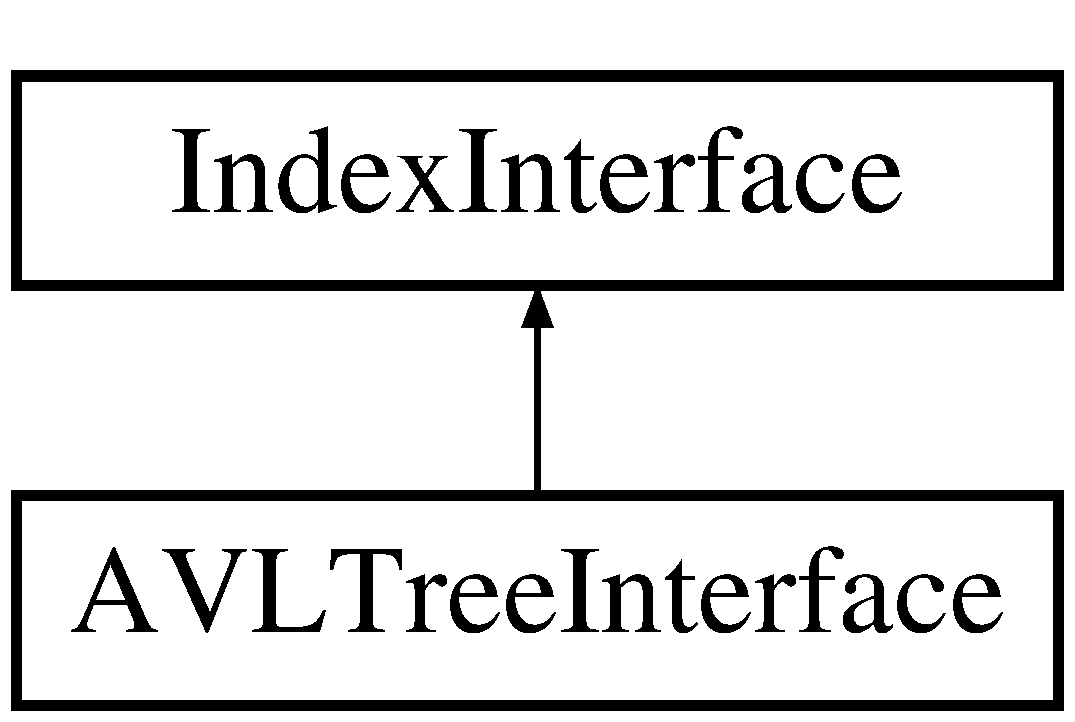
\includegraphics[height=2.000000cm]{class_a_v_l_tree_interface}
\end{center}
\end{figure}
\subsection*{Public Member Functions}
\begin{DoxyCompactItemize}
\item 
\hyperlink{class_a_v_l_tree_interface_abaec1061e3c1982382aeda27495af568}{A\+V\+L\+Tree\+Interface} ()
\begin{DoxyCompactList}\small\item\em constructor \end{DoxyCompactList}\item 
\hyperlink{class_a_v_l_tree_interface_a919ac950421b6702b2f82b9849b81108}{$\sim$\+A\+V\+L\+Tree\+Interface} ()
\begin{DoxyCompactList}\small\item\em destructor \end{DoxyCompactList}\item 
void \hyperlink{class_a_v_l_tree_interface_a2ff7466f1fd70ce6391330c04749fec7}{add\+\_\+term\+\_\+to\+\_\+ii} (int letter\+Index, \hyperlink{class_term}{Term} $\ast$term)
\begin{DoxyCompactList}\small\item\em adds term to the each individual avl\+Trees \end{DoxyCompactList}\item 
void \hyperlink{class_a_v_l_tree_interface_a748ffc895fb64aab3e2afac287f80630}{clear} ()
\begin{DoxyCompactList}\small\item\em clears avl\+Trees \end{DoxyCompactList}\item 
\hyperlink{class_term}{Term} $\ast$ \hyperlink{class_a_v_l_tree_interface_a35ee941b125e65cf0b5783a687503d83}{find\+\_\+term} (string term)
\begin{DoxyCompactList}\small\item\em searches each avl\+Trees for word and than returns term \end{DoxyCompactList}\item 
void \hyperlink{class_a_v_l_tree_interface_abd7f70746611a3982dc07a1b1880e7b5}{write\+\_\+persistence\+\_\+files} ()
\begin{DoxyCompactList}\small\item\em creates the persistance index \end{DoxyCompactList}\item 
void \hyperlink{class_index_interface_a7f082789ce91eaaacc10a5c841b62cd4}{append\+\_\+page\+\_\+info} (\hyperlink{class_page_info}{Page\+Info} $\ast$curr\+Info)
\item 
double \hyperlink{class_index_interface_a8195aee88cd593c2e6ca2e2c48cbd068}{calc\+\_\+tdidf} (int page\+I\+D, int freq, int spread)
\item 
void \hyperlink{class_index_interface_a7e4d5fe8c31cfc9aa02c2dd1d7e1d3aa}{display\+\_\+result} (int rank, int page\+I\+D, double tdidf)
\item 
void \hyperlink{class_index_interface_a3d784385e028557312ef15d59574f9ed}{display\+\_\+page\+\_\+content} (int page\+I\+D)
\item 
void \hyperlink{class_index_interface_a5734b1488a787d47984bf97ffa5aff8d}{incr\+\_\+total\+\_\+words\+\_\+on\+\_\+page} (int curr\+I\+D, int incr)
\item 
void \hyperlink{class_index_interface_a229f1eb93f38d85d78e64e579c46c98a}{read\+\_\+file} (string file\+Path)
\item 
void \hyperlink{class_index_interface_aa6ef58f8b651083175b684b9428a90c5}{read\+\_\+persistence\+\_\+files} (\hyperlink{docparser_8h_a9b942645c404d380838be4078b0199d9}{term\+Map} \&all\+Terms)
\item 
void \hyperlink{class_index_interface_adcba07c90cd34ab0ce7bee340d09ed07}{read\+\_\+pers\+\_\+file} (int index, \hyperlink{docparser_8h_a9b942645c404d380838be4078b0199d9}{term\+Map} \&all\+Terms)
\item 
int \hyperlink{class_index_interface_a9a7539d9c7a48bf4d4fbe43961c0547f}{index\+\_\+for\+\_\+letter} (char letter)
\item 
\hyperlink{class_page_info}{Page\+Info} $\ast$ \hyperlink{class_index_interface_a2af7d88c3b2701be9164ba9f4a3bddb3}{info\+\_\+for\+\_\+page\+I\+D} (int page\+I\+D)
\item 
int \hyperlink{class_index_interface_a8a0132ad6e84c4340061496c615f581c}{get\+\_\+total\+Words\+In\+Corpus} ()
\item 
int \hyperlink{class_index_interface_af9edc24ac00bdf2c0e06384f890a1d8a}{get\+\_\+total\+Pages} ()
\end{DoxyCompactItemize}
\subsection*{Protected Attributes}
\begin{DoxyCompactItemize}
\item 
\hyperlink{class_hash_table_index}{Hash\+Table\+Index} $\ast$ \hyperlink{class_index_interface_a8511509bb58da989f705ba75fd5dde2d}{letters}
\item 
vector$<$ \hyperlink{class_page_info}{Page\+Info} $\ast$ $>$ \hyperlink{class_index_interface_a8400a62750faa69ff35308ff731d9ee5}{info\+For\+I\+Ds}
\item 
\hyperlink{class_doc_parser}{Doc\+Parser} \& \hyperlink{class_index_interface_a42b0d9eccd309185ed92976f72908bb9}{parser}
\item 
int \hyperlink{class_index_interface_a2df695d2b504f2e53a0bfdd6bfee31da}{total\+Pages}
\item 
int \hyperlink{class_index_interface_ab607b430e78528cdb8bb79ba4afa91d2}{total\+Words\+In\+Corpus}
\end{DoxyCompactItemize}
\subsection*{Private Attributes}
\begin{DoxyCompactItemize}
\item 
\hyperlink{class_a_v_l_tree_index}{A\+V\+L\+Tree\+Index} $\ast$ \hyperlink{class_a_v_l_tree_interface_a1a8fb4dfd2e033e2c9ba24429875e06f}{avl\+Trees}
\begin{DoxyCompactList}\small\item\em creates 26 \hyperlink{class_a_v_l_tree_index}{A\+V\+L\+Tree\+Index}\textquotesingle{}s \end{DoxyCompactList}\item 
const int \hyperlink{class_a_v_l_tree_interface_a198b108f89bc4ef2eefae399c1b3b167}{num\+Letters} = 26
\begin{DoxyCompactList}\small\item\em amount of A\+V\+L Trees \end{DoxyCompactList}\end{DoxyCompactItemize}


\subsection{Detailed Description}
A\+V\+L Tree \hyperlink{class_interface}{Interface} implements 26 different \hyperlink{class_a_v_l_tree_index}{A\+V\+L\+Tree\+Index}\textquotesingle{}s. 

$<$ inherits virtual functions from \hyperlink{class_index_interface}{Index\+Interface} 

\subsection{Constructor \& Destructor Documentation}
\hypertarget{class_a_v_l_tree_interface_abaec1061e3c1982382aeda27495af568}{}\index{A\+V\+L\+Tree\+Interface@{A\+V\+L\+Tree\+Interface}!A\+V\+L\+Tree\+Interface@{A\+V\+L\+Tree\+Interface}}
\index{A\+V\+L\+Tree\+Interface@{A\+V\+L\+Tree\+Interface}!A\+V\+L\+Tree\+Interface@{A\+V\+L\+Tree\+Interface}}
\subsubsection[{A\+V\+L\+Tree\+Interface}]{\setlength{\rightskip}{0pt plus 5cm}A\+V\+L\+Tree\+Interface\+::\+A\+V\+L\+Tree\+Interface (
\begin{DoxyParamCaption}
{}
\end{DoxyParamCaption}
)}\label{class_a_v_l_tree_interface_abaec1061e3c1982382aeda27495af568}


constructor 

\hyperlink{class_a_v_l_tree_interface}{A\+V\+L\+Tree\+Interface} creates 26 different A\+V\+L Trees. \hypertarget{class_a_v_l_tree_interface_a919ac950421b6702b2f82b9849b81108}{}\index{A\+V\+L\+Tree\+Interface@{A\+V\+L\+Tree\+Interface}!````~A\+V\+L\+Tree\+Interface@{$\sim$\+A\+V\+L\+Tree\+Interface}}
\index{````~A\+V\+L\+Tree\+Interface@{$\sim$\+A\+V\+L\+Tree\+Interface}!A\+V\+L\+Tree\+Interface@{A\+V\+L\+Tree\+Interface}}
\subsubsection[{$\sim$\+A\+V\+L\+Tree\+Interface}]{\setlength{\rightskip}{0pt plus 5cm}A\+V\+L\+Tree\+Interface\+::$\sim$\+A\+V\+L\+Tree\+Interface (
\begin{DoxyParamCaption}
{}
\end{DoxyParamCaption}
)}\label{class_a_v_l_tree_interface_a919ac950421b6702b2f82b9849b81108}


destructor 



\subsection{Member Function Documentation}
\hypertarget{class_a_v_l_tree_interface_a2ff7466f1fd70ce6391330c04749fec7}{}\index{A\+V\+L\+Tree\+Interface@{A\+V\+L\+Tree\+Interface}!add\+\_\+term\+\_\+to\+\_\+ii@{add\+\_\+term\+\_\+to\+\_\+ii}}
\index{add\+\_\+term\+\_\+to\+\_\+ii@{add\+\_\+term\+\_\+to\+\_\+ii}!A\+V\+L\+Tree\+Interface@{A\+V\+L\+Tree\+Interface}}
\subsubsection[{add\+\_\+term\+\_\+to\+\_\+ii}]{\setlength{\rightskip}{0pt plus 5cm}void A\+V\+L\+Tree\+Interface\+::add\+\_\+term\+\_\+to\+\_\+ii (
\begin{DoxyParamCaption}
\item[{int}]{letter\+Index, }
\item[{{\bf Term} $\ast$}]{term}
\end{DoxyParamCaption}
)\hspace{0.3cm}{\ttfamily [virtual]}}\label{class_a_v_l_tree_interface_a2ff7466f1fd70ce6391330c04749fec7}


adds term to the each individual avl\+Trees 



Reimplemented from \hyperlink{class_index_interface_aa83b7083d107869e3519c5862bc71d0a}{Index\+Interface}.

\hypertarget{class_index_interface_a7f082789ce91eaaacc10a5c841b62cd4}{}\index{A\+V\+L\+Tree\+Interface@{A\+V\+L\+Tree\+Interface}!append\+\_\+page\+\_\+info@{append\+\_\+page\+\_\+info}}
\index{append\+\_\+page\+\_\+info@{append\+\_\+page\+\_\+info}!A\+V\+L\+Tree\+Interface@{A\+V\+L\+Tree\+Interface}}
\subsubsection[{append\+\_\+page\+\_\+info}]{\setlength{\rightskip}{0pt plus 5cm}void Index\+Interface\+::append\+\_\+page\+\_\+info (
\begin{DoxyParamCaption}
\item[{{\bf Page\+Info} $\ast$}]{curr\+Info}
\end{DoxyParamCaption}
)\hspace{0.3cm}{\ttfamily [inherited]}}\label{class_index_interface_a7f082789ce91eaaacc10a5c841b62cd4}
\hypertarget{class_index_interface_a8195aee88cd593c2e6ca2e2c48cbd068}{}\index{A\+V\+L\+Tree\+Interface@{A\+V\+L\+Tree\+Interface}!calc\+\_\+tdidf@{calc\+\_\+tdidf}}
\index{calc\+\_\+tdidf@{calc\+\_\+tdidf}!A\+V\+L\+Tree\+Interface@{A\+V\+L\+Tree\+Interface}}
\subsubsection[{calc\+\_\+tdidf}]{\setlength{\rightskip}{0pt plus 5cm}double Index\+Interface\+::calc\+\_\+tdidf (
\begin{DoxyParamCaption}
\item[{int}]{page\+I\+D, }
\item[{int}]{freq, }
\item[{int}]{spread}
\end{DoxyParamCaption}
)\hspace{0.3cm}{\ttfamily [inherited]}}\label{class_index_interface_a8195aee88cd593c2e6ca2e2c48cbd068}
\hypertarget{class_a_v_l_tree_interface_a748ffc895fb64aab3e2afac287f80630}{}\index{A\+V\+L\+Tree\+Interface@{A\+V\+L\+Tree\+Interface}!clear@{clear}}
\index{clear@{clear}!A\+V\+L\+Tree\+Interface@{A\+V\+L\+Tree\+Interface}}
\subsubsection[{clear}]{\setlength{\rightskip}{0pt plus 5cm}void A\+V\+L\+Tree\+Interface\+::clear (
\begin{DoxyParamCaption}
{}
\end{DoxyParamCaption}
)\hspace{0.3cm}{\ttfamily [virtual]}}\label{class_a_v_l_tree_interface_a748ffc895fb64aab3e2afac287f80630}


clears avl\+Trees 



Reimplemented from \hyperlink{class_index_interface_ad7b88501f360ccfad0c1ee08d793ca25}{Index\+Interface}.

\hypertarget{class_index_interface_a3d784385e028557312ef15d59574f9ed}{}\index{A\+V\+L\+Tree\+Interface@{A\+V\+L\+Tree\+Interface}!display\+\_\+page\+\_\+content@{display\+\_\+page\+\_\+content}}
\index{display\+\_\+page\+\_\+content@{display\+\_\+page\+\_\+content}!A\+V\+L\+Tree\+Interface@{A\+V\+L\+Tree\+Interface}}
\subsubsection[{display\+\_\+page\+\_\+content}]{\setlength{\rightskip}{0pt plus 5cm}void Index\+Interface\+::display\+\_\+page\+\_\+content (
\begin{DoxyParamCaption}
\item[{int}]{page\+I\+D}
\end{DoxyParamCaption}
)\hspace{0.3cm}{\ttfamily [inherited]}}\label{class_index_interface_a3d784385e028557312ef15d59574f9ed}
\hypertarget{class_index_interface_a7e4d5fe8c31cfc9aa02c2dd1d7e1d3aa}{}\index{A\+V\+L\+Tree\+Interface@{A\+V\+L\+Tree\+Interface}!display\+\_\+result@{display\+\_\+result}}
\index{display\+\_\+result@{display\+\_\+result}!A\+V\+L\+Tree\+Interface@{A\+V\+L\+Tree\+Interface}}
\subsubsection[{display\+\_\+result}]{\setlength{\rightskip}{0pt plus 5cm}void Index\+Interface\+::display\+\_\+result (
\begin{DoxyParamCaption}
\item[{int}]{rank, }
\item[{int}]{page\+I\+D, }
\item[{double}]{tdidf}
\end{DoxyParamCaption}
)\hspace{0.3cm}{\ttfamily [inherited]}}\label{class_index_interface_a7e4d5fe8c31cfc9aa02c2dd1d7e1d3aa}
\hypertarget{class_a_v_l_tree_interface_a35ee941b125e65cf0b5783a687503d83}{}\index{A\+V\+L\+Tree\+Interface@{A\+V\+L\+Tree\+Interface}!find\+\_\+term@{find\+\_\+term}}
\index{find\+\_\+term@{find\+\_\+term}!A\+V\+L\+Tree\+Interface@{A\+V\+L\+Tree\+Interface}}
\subsubsection[{find\+\_\+term}]{\setlength{\rightskip}{0pt plus 5cm}{\bf Term} $\ast$ A\+V\+L\+Tree\+Interface\+::find\+\_\+term (
\begin{DoxyParamCaption}
\item[{string}]{term}
\end{DoxyParamCaption}
)\hspace{0.3cm}{\ttfamily [virtual]}}\label{class_a_v_l_tree_interface_a35ee941b125e65cf0b5783a687503d83}


searches each avl\+Trees for word and than returns term 



Reimplemented from \hyperlink{class_index_interface_a851f0396f0b390cc9aa8cde270afffc9}{Index\+Interface}.

\hypertarget{class_index_interface_af9edc24ac00bdf2c0e06384f890a1d8a}{}\index{A\+V\+L\+Tree\+Interface@{A\+V\+L\+Tree\+Interface}!get\+\_\+total\+Pages@{get\+\_\+total\+Pages}}
\index{get\+\_\+total\+Pages@{get\+\_\+total\+Pages}!A\+V\+L\+Tree\+Interface@{A\+V\+L\+Tree\+Interface}}
\subsubsection[{get\+\_\+total\+Pages}]{\setlength{\rightskip}{0pt plus 5cm}int Index\+Interface\+::get\+\_\+total\+Pages (
\begin{DoxyParamCaption}
{}
\end{DoxyParamCaption}
)\hspace{0.3cm}{\ttfamily [inherited]}}\label{class_index_interface_af9edc24ac00bdf2c0e06384f890a1d8a}
\hypertarget{class_index_interface_a8a0132ad6e84c4340061496c615f581c}{}\index{A\+V\+L\+Tree\+Interface@{A\+V\+L\+Tree\+Interface}!get\+\_\+total\+Words\+In\+Corpus@{get\+\_\+total\+Words\+In\+Corpus}}
\index{get\+\_\+total\+Words\+In\+Corpus@{get\+\_\+total\+Words\+In\+Corpus}!A\+V\+L\+Tree\+Interface@{A\+V\+L\+Tree\+Interface}}
\subsubsection[{get\+\_\+total\+Words\+In\+Corpus}]{\setlength{\rightskip}{0pt plus 5cm}int Index\+Interface\+::get\+\_\+total\+Words\+In\+Corpus (
\begin{DoxyParamCaption}
{}
\end{DoxyParamCaption}
)\hspace{0.3cm}{\ttfamily [inherited]}}\label{class_index_interface_a8a0132ad6e84c4340061496c615f581c}
\hypertarget{class_index_interface_a5734b1488a787d47984bf97ffa5aff8d}{}\index{A\+V\+L\+Tree\+Interface@{A\+V\+L\+Tree\+Interface}!incr\+\_\+total\+\_\+words\+\_\+on\+\_\+page@{incr\+\_\+total\+\_\+words\+\_\+on\+\_\+page}}
\index{incr\+\_\+total\+\_\+words\+\_\+on\+\_\+page@{incr\+\_\+total\+\_\+words\+\_\+on\+\_\+page}!A\+V\+L\+Tree\+Interface@{A\+V\+L\+Tree\+Interface}}
\subsubsection[{incr\+\_\+total\+\_\+words\+\_\+on\+\_\+page}]{\setlength{\rightskip}{0pt plus 5cm}void Index\+Interface\+::incr\+\_\+total\+\_\+words\+\_\+on\+\_\+page (
\begin{DoxyParamCaption}
\item[{int}]{curr\+I\+D, }
\item[{int}]{incr}
\end{DoxyParamCaption}
)\hspace{0.3cm}{\ttfamily [inherited]}}\label{class_index_interface_a5734b1488a787d47984bf97ffa5aff8d}
\hypertarget{class_index_interface_a9a7539d9c7a48bf4d4fbe43961c0547f}{}\index{A\+V\+L\+Tree\+Interface@{A\+V\+L\+Tree\+Interface}!index\+\_\+for\+\_\+letter@{index\+\_\+for\+\_\+letter}}
\index{index\+\_\+for\+\_\+letter@{index\+\_\+for\+\_\+letter}!A\+V\+L\+Tree\+Interface@{A\+V\+L\+Tree\+Interface}}
\subsubsection[{index\+\_\+for\+\_\+letter}]{\setlength{\rightskip}{0pt plus 5cm}int Index\+Interface\+::index\+\_\+for\+\_\+letter (
\begin{DoxyParamCaption}
\item[{char}]{letter}
\end{DoxyParamCaption}
)\hspace{0.3cm}{\ttfamily [inherited]}}\label{class_index_interface_a9a7539d9c7a48bf4d4fbe43961c0547f}
\hypertarget{class_index_interface_a2af7d88c3b2701be9164ba9f4a3bddb3}{}\index{A\+V\+L\+Tree\+Interface@{A\+V\+L\+Tree\+Interface}!info\+\_\+for\+\_\+page\+I\+D@{info\+\_\+for\+\_\+page\+I\+D}}
\index{info\+\_\+for\+\_\+page\+I\+D@{info\+\_\+for\+\_\+page\+I\+D}!A\+V\+L\+Tree\+Interface@{A\+V\+L\+Tree\+Interface}}
\subsubsection[{info\+\_\+for\+\_\+page\+I\+D}]{\setlength{\rightskip}{0pt plus 5cm}{\bf Page\+Info} $\ast$ Index\+Interface\+::info\+\_\+for\+\_\+page\+I\+D (
\begin{DoxyParamCaption}
\item[{int}]{page\+I\+D}
\end{DoxyParamCaption}
)\hspace{0.3cm}{\ttfamily [inherited]}}\label{class_index_interface_a2af7d88c3b2701be9164ba9f4a3bddb3}
\hypertarget{class_index_interface_a229f1eb93f38d85d78e64e579c46c98a}{}\index{A\+V\+L\+Tree\+Interface@{A\+V\+L\+Tree\+Interface}!read\+\_\+file@{read\+\_\+file}}
\index{read\+\_\+file@{read\+\_\+file}!A\+V\+L\+Tree\+Interface@{A\+V\+L\+Tree\+Interface}}
\subsubsection[{read\+\_\+file}]{\setlength{\rightskip}{0pt plus 5cm}void Index\+Interface\+::read\+\_\+file (
\begin{DoxyParamCaption}
\item[{string}]{file\+Path}
\end{DoxyParamCaption}
)\hspace{0.3cm}{\ttfamily [inherited]}}\label{class_index_interface_a229f1eb93f38d85d78e64e579c46c98a}
\hypertarget{class_index_interface_adcba07c90cd34ab0ce7bee340d09ed07}{}\index{A\+V\+L\+Tree\+Interface@{A\+V\+L\+Tree\+Interface}!read\+\_\+pers\+\_\+file@{read\+\_\+pers\+\_\+file}}
\index{read\+\_\+pers\+\_\+file@{read\+\_\+pers\+\_\+file}!A\+V\+L\+Tree\+Interface@{A\+V\+L\+Tree\+Interface}}
\subsubsection[{read\+\_\+pers\+\_\+file}]{\setlength{\rightskip}{0pt plus 5cm}void Index\+Interface\+::read\+\_\+pers\+\_\+file (
\begin{DoxyParamCaption}
\item[{int}]{index, }
\item[{{\bf term\+Map} \&}]{all\+Terms}
\end{DoxyParamCaption}
)\hspace{0.3cm}{\ttfamily [inherited]}}\label{class_index_interface_adcba07c90cd34ab0ce7bee340d09ed07}
\hypertarget{class_index_interface_aa6ef58f8b651083175b684b9428a90c5}{}\index{A\+V\+L\+Tree\+Interface@{A\+V\+L\+Tree\+Interface}!read\+\_\+persistence\+\_\+files@{read\+\_\+persistence\+\_\+files}}
\index{read\+\_\+persistence\+\_\+files@{read\+\_\+persistence\+\_\+files}!A\+V\+L\+Tree\+Interface@{A\+V\+L\+Tree\+Interface}}
\subsubsection[{read\+\_\+persistence\+\_\+files}]{\setlength{\rightskip}{0pt plus 5cm}void Index\+Interface\+::read\+\_\+persistence\+\_\+files (
\begin{DoxyParamCaption}
\item[{{\bf term\+Map} \&}]{all\+Terms}
\end{DoxyParamCaption}
)\hspace{0.3cm}{\ttfamily [inherited]}}\label{class_index_interface_aa6ef58f8b651083175b684b9428a90c5}
\hypertarget{class_a_v_l_tree_interface_abd7f70746611a3982dc07a1b1880e7b5}{}\index{A\+V\+L\+Tree\+Interface@{A\+V\+L\+Tree\+Interface}!write\+\_\+persistence\+\_\+files@{write\+\_\+persistence\+\_\+files}}
\index{write\+\_\+persistence\+\_\+files@{write\+\_\+persistence\+\_\+files}!A\+V\+L\+Tree\+Interface@{A\+V\+L\+Tree\+Interface}}
\subsubsection[{write\+\_\+persistence\+\_\+files}]{\setlength{\rightskip}{0pt plus 5cm}void A\+V\+L\+Tree\+Interface\+::write\+\_\+persistence\+\_\+files (
\begin{DoxyParamCaption}
{}
\end{DoxyParamCaption}
)\hspace{0.3cm}{\ttfamily [virtual]}}\label{class_a_v_l_tree_interface_abd7f70746611a3982dc07a1b1880e7b5}


creates the persistance index 



Reimplemented from \hyperlink{class_index_interface_a0b4ec5fcc32c08959cffad3a3141dd4e}{Index\+Interface}.



\subsection{Member Data Documentation}
\hypertarget{class_a_v_l_tree_interface_a1a8fb4dfd2e033e2c9ba24429875e06f}{}\index{A\+V\+L\+Tree\+Interface@{A\+V\+L\+Tree\+Interface}!avl\+Trees@{avl\+Trees}}
\index{avl\+Trees@{avl\+Trees}!A\+V\+L\+Tree\+Interface@{A\+V\+L\+Tree\+Interface}}
\subsubsection[{avl\+Trees}]{\setlength{\rightskip}{0pt plus 5cm}{\bf A\+V\+L\+Tree\+Index}$\ast$ A\+V\+L\+Tree\+Interface\+::avl\+Trees\hspace{0.3cm}{\ttfamily [private]}}\label{class_a_v_l_tree_interface_a1a8fb4dfd2e033e2c9ba24429875e06f}


creates 26 \hyperlink{class_a_v_l_tree_index}{A\+V\+L\+Tree\+Index}\textquotesingle{}s 

\hypertarget{class_index_interface_a8400a62750faa69ff35308ff731d9ee5}{}\index{A\+V\+L\+Tree\+Interface@{A\+V\+L\+Tree\+Interface}!info\+For\+I\+Ds@{info\+For\+I\+Ds}}
\index{info\+For\+I\+Ds@{info\+For\+I\+Ds}!A\+V\+L\+Tree\+Interface@{A\+V\+L\+Tree\+Interface}}
\subsubsection[{info\+For\+I\+Ds}]{\setlength{\rightskip}{0pt plus 5cm}vector$<${\bf Page\+Info}$\ast$$>$ Index\+Interface\+::info\+For\+I\+Ds\hspace{0.3cm}{\ttfamily [protected]}, {\ttfamily [inherited]}}\label{class_index_interface_a8400a62750faa69ff35308ff731d9ee5}
\hypertarget{class_index_interface_a8511509bb58da989f705ba75fd5dde2d}{}\index{A\+V\+L\+Tree\+Interface@{A\+V\+L\+Tree\+Interface}!letters@{letters}}
\index{letters@{letters}!A\+V\+L\+Tree\+Interface@{A\+V\+L\+Tree\+Interface}}
\subsubsection[{letters}]{\setlength{\rightskip}{0pt plus 5cm}{\bf Hash\+Table\+Index}$\ast$ Index\+Interface\+::letters\hspace{0.3cm}{\ttfamily [protected]}, {\ttfamily [inherited]}}\label{class_index_interface_a8511509bb58da989f705ba75fd5dde2d}
\hypertarget{class_a_v_l_tree_interface_a198b108f89bc4ef2eefae399c1b3b167}{}\index{A\+V\+L\+Tree\+Interface@{A\+V\+L\+Tree\+Interface}!num\+Letters@{num\+Letters}}
\index{num\+Letters@{num\+Letters}!A\+V\+L\+Tree\+Interface@{A\+V\+L\+Tree\+Interface}}
\subsubsection[{num\+Letters}]{\setlength{\rightskip}{0pt plus 5cm}const int A\+V\+L\+Tree\+Interface\+::num\+Letters = 26\hspace{0.3cm}{\ttfamily [private]}}\label{class_a_v_l_tree_interface_a198b108f89bc4ef2eefae399c1b3b167}


amount of A\+V\+L Trees 

\hypertarget{class_index_interface_a42b0d9eccd309185ed92976f72908bb9}{}\index{A\+V\+L\+Tree\+Interface@{A\+V\+L\+Tree\+Interface}!parser@{parser}}
\index{parser@{parser}!A\+V\+L\+Tree\+Interface@{A\+V\+L\+Tree\+Interface}}
\subsubsection[{parser}]{\setlength{\rightskip}{0pt plus 5cm}{\bf Doc\+Parser}\& Index\+Interface\+::parser\hspace{0.3cm}{\ttfamily [protected]}, {\ttfamily [inherited]}}\label{class_index_interface_a42b0d9eccd309185ed92976f72908bb9}
\hypertarget{class_index_interface_a2df695d2b504f2e53a0bfdd6bfee31da}{}\index{A\+V\+L\+Tree\+Interface@{A\+V\+L\+Tree\+Interface}!total\+Pages@{total\+Pages}}
\index{total\+Pages@{total\+Pages}!A\+V\+L\+Tree\+Interface@{A\+V\+L\+Tree\+Interface}}
\subsubsection[{total\+Pages}]{\setlength{\rightskip}{0pt plus 5cm}int Index\+Interface\+::total\+Pages\hspace{0.3cm}{\ttfamily [protected]}, {\ttfamily [inherited]}}\label{class_index_interface_a2df695d2b504f2e53a0bfdd6bfee31da}
\hypertarget{class_index_interface_ab607b430e78528cdb8bb79ba4afa91d2}{}\index{A\+V\+L\+Tree\+Interface@{A\+V\+L\+Tree\+Interface}!total\+Words\+In\+Corpus@{total\+Words\+In\+Corpus}}
\index{total\+Words\+In\+Corpus@{total\+Words\+In\+Corpus}!A\+V\+L\+Tree\+Interface@{A\+V\+L\+Tree\+Interface}}
\subsubsection[{total\+Words\+In\+Corpus}]{\setlength{\rightskip}{0pt plus 5cm}int Index\+Interface\+::total\+Words\+In\+Corpus\hspace{0.3cm}{\ttfamily [protected]}, {\ttfamily [inherited]}}\label{class_index_interface_ab607b430e78528cdb8bb79ba4afa91d2}


The documentation for this class was generated from the following files\+:\begin{DoxyCompactItemize}
\item 
\hyperlink{avltreeinterface_8h}{avltreeinterface.\+h}\item 
\hyperlink{avltreeinterface_8cpp}{avltreeinterface.\+cpp}\end{DoxyCompactItemize}

\hypertarget{class_doc_parser}{}\section{Doc\+Parser Class Reference}
\label{class_doc_parser}\index{Doc\+Parser@{Doc\+Parser}}


Uses rapidxml to parse throught the wiki\+Dump.  




{\ttfamily \#include $<$docparser.\+h$>$}

\subsection*{Public Member Functions}
\begin{DoxyCompactItemize}
\item 
\hyperlink{class_doc_parser_a637fc4d565eaf2927ee9b88bbe23e3cb}{$\sim$\+Doc\+Parser} ()
\item 
\hyperlink{class_doc_parser_a086f00e54fca8038c85c0e235948d75a}{Doc\+Parser} (\hyperlink{class_index_interface}{Index\+Interface} \&the\+Index)
\item 
string \hyperlink{class_doc_parser_a1b127af53e8af16f393b64f46c307d3a}{clean\+\_\+term} (string term)
\item 
void \hyperlink{class_doc_parser_ad92d1a6da7d413abd27ee18a6ed20a30}{clear} ()
\item 
int \hyperlink{class_doc_parser_a7addc81ac337c2688bb9e9d8197db2fc}{index\+\_\+for\+\_\+letter} (char letter)
\item 
void \hyperlink{class_doc_parser_a48cd3949baca573b9be0b4ba24b9c79d}{read\+\_\+page} (\hyperlink{classrapidxml_1_1xml__node}{xml\+\_\+node}$<$$>$ $\ast$curr\+Node, bool read\+Text)
\item 
void \hyperlink{class_doc_parser_af28153ebf0ee2fe97c2942c04c915adc}{read\+\_\+text} (\hyperlink{classrapidxml_1_1xml__node}{xml\+\_\+node}$<$$>$ $\ast$curr\+Node)
\item 
void \hyperlink{class_doc_parser_ad7b5809e4efd3e2bae781c1cb491ab29}{init\+\_\+file\+\_\+page\+\_\+infos} (\hyperlink{classrapidxml_1_1xml__node}{xml\+\_\+node}$<$$>$ $\ast$curr\+Node, bool read\+Text)
\item 
void \hyperlink{class_doc_parser_a45860ee7fb0b956c4342cd4a815818de}{read\+\_\+file} (string file\+Path)
\item 
bool \hyperlink{class_doc_parser_ad30c49de12ed45eaf2594c4718789c3e}{is\+\_\+stop\+\_\+word} (string term)
\end{DoxyCompactItemize}
\subsection*{Private Attributes}
\begin{DoxyCompactItemize}
\item 
\hyperlink{class_index_interface}{Index\+Interface} \& \hyperlink{class_doc_parser_ad0e840d5c92edbe2c8f28406a5c3f008}{index}
\item 
\hyperlink{docparser_8h_aa63707b94c556a8d9df334f564b61b0b}{stop\+Word\+Map} \hyperlink{class_doc_parser_a089705924f6a28afb59064526b4b7f4f}{stop\+Words}
\item 
int \hyperlink{class_doc_parser_ace9019a4f9ede433886adaa0656e6e3b}{count} = 0
\item 
string \hyperlink{class_doc_parser_a03b27a633885e614c94635eb2f66d404}{curr\+Word}
\item 
string \hyperlink{class_doc_parser_aaf8b70c4ddd9637f3e700f42a88fb641}{curr\+Content}
\item 
string \hyperlink{class_doc_parser_acf0aedb227a48a682d1ff238d1d6614d}{curr\+Contributor\+Name\+Or\+I\+P}
\item 
string \hyperlink{class_doc_parser_a642bcf2a542abd6b386c1445e937e4cd}{curr\+Timestamp}
\item 
string \hyperlink{class_doc_parser_a8348dc55e8aa858bbc5becc02d4e53bf}{curr\+Title}
\item 
\hyperlink{class_term}{Term} $\ast$ \hyperlink{class_doc_parser_adb6f140f5f0972129201a0f7fe4be541}{found}
\end{DoxyCompactItemize}


\subsection{Detailed Description}
Uses rapidxml to parse throught the wiki\+Dump. 

\subsection{Constructor \& Destructor Documentation}
\hypertarget{class_doc_parser_a637fc4d565eaf2927ee9b88bbe23e3cb}{}\index{Doc\+Parser@{Doc\+Parser}!````~Doc\+Parser@{$\sim$\+Doc\+Parser}}
\index{````~Doc\+Parser@{$\sim$\+Doc\+Parser}!Doc\+Parser@{Doc\+Parser}}
\subsubsection[{$\sim$\+Doc\+Parser}]{\setlength{\rightskip}{0pt plus 5cm}Doc\+Parser\+::$\sim$\+Doc\+Parser (
\begin{DoxyParamCaption}
{}
\end{DoxyParamCaption}
)}\label{class_doc_parser_a637fc4d565eaf2927ee9b88bbe23e3cb}
\hypertarget{class_doc_parser_a086f00e54fca8038c85c0e235948d75a}{}\index{Doc\+Parser@{Doc\+Parser}!Doc\+Parser@{Doc\+Parser}}
\index{Doc\+Parser@{Doc\+Parser}!Doc\+Parser@{Doc\+Parser}}
\subsubsection[{Doc\+Parser}]{\setlength{\rightskip}{0pt plus 5cm}Doc\+Parser\+::\+Doc\+Parser (
\begin{DoxyParamCaption}
\item[{{\bf Index\+Interface} \&}]{the\+Index}
\end{DoxyParamCaption}
)}\label{class_doc_parser_a086f00e54fca8038c85c0e235948d75a}


\subsection{Member Function Documentation}
\hypertarget{class_doc_parser_a1b127af53e8af16f393b64f46c307d3a}{}\index{Doc\+Parser@{Doc\+Parser}!clean\+\_\+term@{clean\+\_\+term}}
\index{clean\+\_\+term@{clean\+\_\+term}!Doc\+Parser@{Doc\+Parser}}
\subsubsection[{clean\+\_\+term}]{\setlength{\rightskip}{0pt plus 5cm}string Doc\+Parser\+::clean\+\_\+term (
\begin{DoxyParamCaption}
\item[{string}]{term}
\end{DoxyParamCaption}
)}\label{class_doc_parser_a1b127af53e8af16f393b64f46c307d3a}
\hypertarget{class_doc_parser_ad92d1a6da7d413abd27ee18a6ed20a30}{}\index{Doc\+Parser@{Doc\+Parser}!clear@{clear}}
\index{clear@{clear}!Doc\+Parser@{Doc\+Parser}}
\subsubsection[{clear}]{\setlength{\rightskip}{0pt plus 5cm}void Doc\+Parser\+::clear (
\begin{DoxyParamCaption}
{}
\end{DoxyParamCaption}
)}\label{class_doc_parser_ad92d1a6da7d413abd27ee18a6ed20a30}
\hypertarget{class_doc_parser_a7addc81ac337c2688bb9e9d8197db2fc}{}\index{Doc\+Parser@{Doc\+Parser}!index\+\_\+for\+\_\+letter@{index\+\_\+for\+\_\+letter}}
\index{index\+\_\+for\+\_\+letter@{index\+\_\+for\+\_\+letter}!Doc\+Parser@{Doc\+Parser}}
\subsubsection[{index\+\_\+for\+\_\+letter}]{\setlength{\rightskip}{0pt plus 5cm}int Doc\+Parser\+::index\+\_\+for\+\_\+letter (
\begin{DoxyParamCaption}
\item[{char}]{letter}
\end{DoxyParamCaption}
)}\label{class_doc_parser_a7addc81ac337c2688bb9e9d8197db2fc}
\hypertarget{class_doc_parser_ad7b5809e4efd3e2bae781c1cb491ab29}{}\index{Doc\+Parser@{Doc\+Parser}!init\+\_\+file\+\_\+page\+\_\+infos@{init\+\_\+file\+\_\+page\+\_\+infos}}
\index{init\+\_\+file\+\_\+page\+\_\+infos@{init\+\_\+file\+\_\+page\+\_\+infos}!Doc\+Parser@{Doc\+Parser}}
\subsubsection[{init\+\_\+file\+\_\+page\+\_\+infos}]{\setlength{\rightskip}{0pt plus 5cm}void Doc\+Parser\+::init\+\_\+file\+\_\+page\+\_\+infos (
\begin{DoxyParamCaption}
\item[{{\bf xml\+\_\+node}$<$$>$ $\ast$}]{curr\+Node, }
\item[{bool}]{read\+Text}
\end{DoxyParamCaption}
)}\label{class_doc_parser_ad7b5809e4efd3e2bae781c1cb491ab29}
\hypertarget{class_doc_parser_ad30c49de12ed45eaf2594c4718789c3e}{}\index{Doc\+Parser@{Doc\+Parser}!is\+\_\+stop\+\_\+word@{is\+\_\+stop\+\_\+word}}
\index{is\+\_\+stop\+\_\+word@{is\+\_\+stop\+\_\+word}!Doc\+Parser@{Doc\+Parser}}
\subsubsection[{is\+\_\+stop\+\_\+word}]{\setlength{\rightskip}{0pt plus 5cm}bool Doc\+Parser\+::is\+\_\+stop\+\_\+word (
\begin{DoxyParamCaption}
\item[{string}]{term}
\end{DoxyParamCaption}
)}\label{class_doc_parser_ad30c49de12ed45eaf2594c4718789c3e}
\hypertarget{class_doc_parser_a45860ee7fb0b956c4342cd4a815818de}{}\index{Doc\+Parser@{Doc\+Parser}!read\+\_\+file@{read\+\_\+file}}
\index{read\+\_\+file@{read\+\_\+file}!Doc\+Parser@{Doc\+Parser}}
\subsubsection[{read\+\_\+file}]{\setlength{\rightskip}{0pt plus 5cm}void Doc\+Parser\+::read\+\_\+file (
\begin{DoxyParamCaption}
\item[{string}]{file\+Path}
\end{DoxyParamCaption}
)}\label{class_doc_parser_a45860ee7fb0b956c4342cd4a815818de}
\hypertarget{class_doc_parser_a48cd3949baca573b9be0b4ba24b9c79d}{}\index{Doc\+Parser@{Doc\+Parser}!read\+\_\+page@{read\+\_\+page}}
\index{read\+\_\+page@{read\+\_\+page}!Doc\+Parser@{Doc\+Parser}}
\subsubsection[{read\+\_\+page}]{\setlength{\rightskip}{0pt plus 5cm}void Doc\+Parser\+::read\+\_\+page (
\begin{DoxyParamCaption}
\item[{{\bf xml\+\_\+node}$<$$>$ $\ast$}]{curr\+Node, }
\item[{bool}]{read\+Text}
\end{DoxyParamCaption}
)}\label{class_doc_parser_a48cd3949baca573b9be0b4ba24b9c79d}
\hypertarget{class_doc_parser_af28153ebf0ee2fe97c2942c04c915adc}{}\index{Doc\+Parser@{Doc\+Parser}!read\+\_\+text@{read\+\_\+text}}
\index{read\+\_\+text@{read\+\_\+text}!Doc\+Parser@{Doc\+Parser}}
\subsubsection[{read\+\_\+text}]{\setlength{\rightskip}{0pt plus 5cm}void Doc\+Parser\+::read\+\_\+text (
\begin{DoxyParamCaption}
\item[{{\bf xml\+\_\+node}$<$$>$ $\ast$}]{curr\+Node}
\end{DoxyParamCaption}
)}\label{class_doc_parser_af28153ebf0ee2fe97c2942c04c915adc}


\subsection{Member Data Documentation}
\hypertarget{class_doc_parser_ace9019a4f9ede433886adaa0656e6e3b}{}\index{Doc\+Parser@{Doc\+Parser}!count@{count}}
\index{count@{count}!Doc\+Parser@{Doc\+Parser}}
\subsubsection[{count}]{\setlength{\rightskip}{0pt plus 5cm}int Doc\+Parser\+::count = 0\hspace{0.3cm}{\ttfamily [private]}}\label{class_doc_parser_ace9019a4f9ede433886adaa0656e6e3b}
\hypertarget{class_doc_parser_aaf8b70c4ddd9637f3e700f42a88fb641}{}\index{Doc\+Parser@{Doc\+Parser}!curr\+Content@{curr\+Content}}
\index{curr\+Content@{curr\+Content}!Doc\+Parser@{Doc\+Parser}}
\subsubsection[{curr\+Content}]{\setlength{\rightskip}{0pt plus 5cm}string Doc\+Parser\+::curr\+Content\hspace{0.3cm}{\ttfamily [private]}}\label{class_doc_parser_aaf8b70c4ddd9637f3e700f42a88fb641}
\hypertarget{class_doc_parser_acf0aedb227a48a682d1ff238d1d6614d}{}\index{Doc\+Parser@{Doc\+Parser}!curr\+Contributor\+Name\+Or\+I\+P@{curr\+Contributor\+Name\+Or\+I\+P}}
\index{curr\+Contributor\+Name\+Or\+I\+P@{curr\+Contributor\+Name\+Or\+I\+P}!Doc\+Parser@{Doc\+Parser}}
\subsubsection[{curr\+Contributor\+Name\+Or\+I\+P}]{\setlength{\rightskip}{0pt plus 5cm}string Doc\+Parser\+::curr\+Contributor\+Name\+Or\+I\+P\hspace{0.3cm}{\ttfamily [private]}}\label{class_doc_parser_acf0aedb227a48a682d1ff238d1d6614d}
\hypertarget{class_doc_parser_a642bcf2a542abd6b386c1445e937e4cd}{}\index{Doc\+Parser@{Doc\+Parser}!curr\+Timestamp@{curr\+Timestamp}}
\index{curr\+Timestamp@{curr\+Timestamp}!Doc\+Parser@{Doc\+Parser}}
\subsubsection[{curr\+Timestamp}]{\setlength{\rightskip}{0pt plus 5cm}string Doc\+Parser\+::curr\+Timestamp\hspace{0.3cm}{\ttfamily [private]}}\label{class_doc_parser_a642bcf2a542abd6b386c1445e937e4cd}
\hypertarget{class_doc_parser_a8348dc55e8aa858bbc5becc02d4e53bf}{}\index{Doc\+Parser@{Doc\+Parser}!curr\+Title@{curr\+Title}}
\index{curr\+Title@{curr\+Title}!Doc\+Parser@{Doc\+Parser}}
\subsubsection[{curr\+Title}]{\setlength{\rightskip}{0pt plus 5cm}string Doc\+Parser\+::curr\+Title\hspace{0.3cm}{\ttfamily [private]}}\label{class_doc_parser_a8348dc55e8aa858bbc5becc02d4e53bf}
\hypertarget{class_doc_parser_a03b27a633885e614c94635eb2f66d404}{}\index{Doc\+Parser@{Doc\+Parser}!curr\+Word@{curr\+Word}}
\index{curr\+Word@{curr\+Word}!Doc\+Parser@{Doc\+Parser}}
\subsubsection[{curr\+Word}]{\setlength{\rightskip}{0pt plus 5cm}string Doc\+Parser\+::curr\+Word\hspace{0.3cm}{\ttfamily [private]}}\label{class_doc_parser_a03b27a633885e614c94635eb2f66d404}
\hypertarget{class_doc_parser_adb6f140f5f0972129201a0f7fe4be541}{}\index{Doc\+Parser@{Doc\+Parser}!found@{found}}
\index{found@{found}!Doc\+Parser@{Doc\+Parser}}
\subsubsection[{found}]{\setlength{\rightskip}{0pt plus 5cm}{\bf Term}$\ast$ Doc\+Parser\+::found\hspace{0.3cm}{\ttfamily [private]}}\label{class_doc_parser_adb6f140f5f0972129201a0f7fe4be541}
\hypertarget{class_doc_parser_ad0e840d5c92edbe2c8f28406a5c3f008}{}\index{Doc\+Parser@{Doc\+Parser}!index@{index}}
\index{index@{index}!Doc\+Parser@{Doc\+Parser}}
\subsubsection[{index}]{\setlength{\rightskip}{0pt plus 5cm}{\bf Index\+Interface}\& Doc\+Parser\+::index\hspace{0.3cm}{\ttfamily [private]}}\label{class_doc_parser_ad0e840d5c92edbe2c8f28406a5c3f008}
\hypertarget{class_doc_parser_a089705924f6a28afb59064526b4b7f4f}{}\index{Doc\+Parser@{Doc\+Parser}!stop\+Words@{stop\+Words}}
\index{stop\+Words@{stop\+Words}!Doc\+Parser@{Doc\+Parser}}
\subsubsection[{stop\+Words}]{\setlength{\rightskip}{0pt plus 5cm}{\bf stop\+Word\+Map} Doc\+Parser\+::stop\+Words\hspace{0.3cm}{\ttfamily [private]}}\label{class_doc_parser_a089705924f6a28afb59064526b4b7f4f}


The documentation for this class was generated from the following files\+:\begin{DoxyCompactItemize}
\item 
\hyperlink{docparser_8h}{docparser.\+h}\item 
\hyperlink{docparser_8cpp}{docparser.\+cpp}\end{DoxyCompactItemize}

\hypertarget{classrapidxml_1_1file}{}\section{rapidxml\+:\+:file$<$ Ch $>$ Class Template Reference}
\label{classrapidxml_1_1file}\index{rapidxml\+::file$<$ Ch $>$@{rapidxml\+::file$<$ Ch $>$}}


Represents data loaded from a file.  




{\ttfamily \#include $<$rapidxml\+\_\+utils.\+hpp$>$}

\subsection*{Public Member Functions}
\begin{DoxyCompactItemize}
\item 
\hyperlink{classrapidxml_1_1file_ae881a3cab1fe7152d45c92a8d7606cb3}{file} (const char $\ast$filename)
\item 
\hyperlink{classrapidxml_1_1file_a90707ccd991cc392dcf4bef37eed9d1f}{file} (std\+::basic\+\_\+istream$<$ Ch $>$ \&stream)
\item 
Ch $\ast$ \hyperlink{classrapidxml_1_1file_af1c71d65862c7af14e4708e32a80c1de}{data} ()
\item 
const Ch $\ast$ \hyperlink{classrapidxml_1_1file_aceb8f5ebd577c946a74b1ea3e2e0c576}{data} () const 
\item 
std\+::size\+\_\+t \hyperlink{classrapidxml_1_1file_a20191d167c6e00a88a44ca9a3a54e1c5}{size} () const 
\end{DoxyCompactItemize}
\subsection*{Private Attributes}
\begin{DoxyCompactItemize}
\item 
std\+::vector$<$ Ch $>$ \hyperlink{classrapidxml_1_1file_a60c4a72a55bbf4dbcca07f251a09cddf}{m\+\_\+data}
\end{DoxyCompactItemize}


\subsection{Detailed Description}
\subsubsection*{template$<$class Ch = char$>$class rapidxml\+::file$<$ Ch $>$}

Represents data loaded from a file. 

\subsection{Constructor \& Destructor Documentation}
\hypertarget{classrapidxml_1_1file_ae881a3cab1fe7152d45c92a8d7606cb3}{}\index{rapidxml\+::file@{rapidxml\+::file}!file@{file}}
\index{file@{file}!rapidxml\+::file@{rapidxml\+::file}}
\subsubsection[{file}]{\setlength{\rightskip}{0pt plus 5cm}template$<$class Ch  = char$>$ {\bf rapidxml\+::file}$<$ Ch $>$\+::{\bf file} (
\begin{DoxyParamCaption}
\item[{const char $\ast$}]{filename}
\end{DoxyParamCaption}
)\hspace{0.3cm}{\ttfamily [inline]}}\label{classrapidxml_1_1file_ae881a3cab1fe7152d45c92a8d7606cb3}
Loads file into the memory. Data will be automatically destroyed by the destructor. 
\begin{DoxyParams}{Parameters}
{\em filename} & Filename to load. \\
\hline
\end{DoxyParams}
\hypertarget{classrapidxml_1_1file_a90707ccd991cc392dcf4bef37eed9d1f}{}\index{rapidxml\+::file@{rapidxml\+::file}!file@{file}}
\index{file@{file}!rapidxml\+::file@{rapidxml\+::file}}
\subsubsection[{file}]{\setlength{\rightskip}{0pt plus 5cm}template$<$class Ch  = char$>$ {\bf rapidxml\+::file}$<$ Ch $>$\+::{\bf file} (
\begin{DoxyParamCaption}
\item[{std\+::basic\+\_\+istream$<$ Ch $>$ \&}]{stream}
\end{DoxyParamCaption}
)\hspace{0.3cm}{\ttfamily [inline]}}\label{classrapidxml_1_1file_a90707ccd991cc392dcf4bef37eed9d1f}
Loads file into the memory. Data will be automatically destroyed by the destructor 
\begin{DoxyParams}{Parameters}
{\em stream} & Stream to load from \\
\hline
\end{DoxyParams}


\subsection{Member Function Documentation}
\hypertarget{classrapidxml_1_1file_af1c71d65862c7af14e4708e32a80c1de}{}\index{rapidxml\+::file@{rapidxml\+::file}!data@{data}}
\index{data@{data}!rapidxml\+::file@{rapidxml\+::file}}
\subsubsection[{data}]{\setlength{\rightskip}{0pt plus 5cm}template$<$class Ch  = char$>$ Ch$\ast$ {\bf rapidxml\+::file}$<$ Ch $>$\+::data (
\begin{DoxyParamCaption}
{}
\end{DoxyParamCaption}
)\hspace{0.3cm}{\ttfamily [inline]}}\label{classrapidxml_1_1file_af1c71d65862c7af14e4708e32a80c1de}
Gets file data. \begin{DoxyReturn}{Returns}
Pointer to data of file. 
\end{DoxyReturn}
\hypertarget{classrapidxml_1_1file_aceb8f5ebd577c946a74b1ea3e2e0c576}{}\index{rapidxml\+::file@{rapidxml\+::file}!data@{data}}
\index{data@{data}!rapidxml\+::file@{rapidxml\+::file}}
\subsubsection[{data}]{\setlength{\rightskip}{0pt plus 5cm}template$<$class Ch  = char$>$ const Ch$\ast$ {\bf rapidxml\+::file}$<$ Ch $>$\+::data (
\begin{DoxyParamCaption}
{}
\end{DoxyParamCaption}
) const\hspace{0.3cm}{\ttfamily [inline]}}\label{classrapidxml_1_1file_aceb8f5ebd577c946a74b1ea3e2e0c576}
Gets file data. \begin{DoxyReturn}{Returns}
Pointer to data of file. 
\end{DoxyReturn}
\hypertarget{classrapidxml_1_1file_a20191d167c6e00a88a44ca9a3a54e1c5}{}\index{rapidxml\+::file@{rapidxml\+::file}!size@{size}}
\index{size@{size}!rapidxml\+::file@{rapidxml\+::file}}
\subsubsection[{size}]{\setlength{\rightskip}{0pt plus 5cm}template$<$class Ch  = char$>$ std\+::size\+\_\+t {\bf rapidxml\+::file}$<$ Ch $>$\+::size (
\begin{DoxyParamCaption}
{}
\end{DoxyParamCaption}
) const\hspace{0.3cm}{\ttfamily [inline]}}\label{classrapidxml_1_1file_a20191d167c6e00a88a44ca9a3a54e1c5}
Gets file data size. \begin{DoxyReturn}{Returns}
Size of file data, in characters. 
\end{DoxyReturn}


\subsection{Member Data Documentation}
\hypertarget{classrapidxml_1_1file_a60c4a72a55bbf4dbcca07f251a09cddf}{}\index{rapidxml\+::file@{rapidxml\+::file}!m\+\_\+data@{m\+\_\+data}}
\index{m\+\_\+data@{m\+\_\+data}!rapidxml\+::file@{rapidxml\+::file}}
\subsubsection[{m\+\_\+data}]{\setlength{\rightskip}{0pt plus 5cm}template$<$class Ch  = char$>$ std\+::vector$<$Ch$>$ {\bf rapidxml\+::file}$<$ Ch $>$\+::m\+\_\+data\hspace{0.3cm}{\ttfamily [private]}}\label{classrapidxml_1_1file_a60c4a72a55bbf4dbcca07f251a09cddf}


The documentation for this class was generated from the following file\+:\begin{DoxyCompactItemize}
\item 
\hyperlink{rapidxml__utils_8hpp}{rapidxml\+\_\+utils.\+hpp}\end{DoxyCompactItemize}

\hypertarget{class_hash_table_index}{}\section{Hash\+Table\+Index Class Reference}
\label{class_hash_table_index}\index{Hash\+Table\+Index@{Hash\+Table\+Index}}


Hash Table Index implementation for the hash table data structure. connects to term buckets and creates a 1024 of them.  




{\ttfamily \#include $<$hashtableindex.\+h$>$}

\subsection*{Public Member Functions}
\begin{DoxyCompactItemize}
\item 
\hyperlink{class_hash_table_index_a13c1c8deae84226c8bef382adf103b53}{Hash\+Table\+Index} ()
\item 
\hyperlink{class_hash_table_index_af4d2eeae8263c353f91140cb2583fb58}{$\sim$\+Hash\+Table\+Index} ()
\item 
void \hyperlink{class_hash_table_index_a383ac825c3dde6dd2791bb121da7138d}{add\+\_\+term\+\_\+to\+\_\+ht\+\_\+index} (\hyperlink{class_term}{Term} $\ast$term)
\item 
\hyperlink{class_term}{Term} $\ast$ \hyperlink{class_hash_table_index_a5934917eb943ab770d86ab7ff9142aab}{find} (string term)
\item 
int \hyperlink{class_hash_table_index_a93a1393996af092def6a7f2b9156f2c6}{hash\+\_\+key} (string key)
\item 
void \hyperlink{class_hash_table_index_a8ed7978b35943e4b89526bb5d7017f05}{write\+\_\+hti} (ofstream \&persistence)
\item 
void \hyperlink{class_hash_table_index_a253a51a2195d47b3350fdc27fd3d4077}{clear\+\_\+table} ()
\end{DoxyCompactItemize}
\subsection*{Private Attributes}
\begin{DoxyCompactItemize}
\item 
const int \hyperlink{class_hash_table_index_a1b302265c4ce75eb039d82bacd1f4bfd}{arr\+Size} = 1024
\item 
\hyperlink{class_term_bucket}{Term\+Bucket} $\ast$ \hyperlink{class_hash_table_index_a7737d10bb5720666b0bff86376a82a11}{buckets}
\end{DoxyCompactItemize}


\subsection{Detailed Description}
Hash Table Index implementation for the hash table data structure. connects to term buckets and creates a 1024 of them. 

\subsection{Constructor \& Destructor Documentation}
\hypertarget{class_hash_table_index_a13c1c8deae84226c8bef382adf103b53}{}\index{Hash\+Table\+Index@{Hash\+Table\+Index}!Hash\+Table\+Index@{Hash\+Table\+Index}}
\index{Hash\+Table\+Index@{Hash\+Table\+Index}!Hash\+Table\+Index@{Hash\+Table\+Index}}
\subsubsection[{Hash\+Table\+Index}]{\setlength{\rightskip}{0pt plus 5cm}Hash\+Table\+Index\+::\+Hash\+Table\+Index (
\begin{DoxyParamCaption}
{}
\end{DoxyParamCaption}
)}\label{class_hash_table_index_a13c1c8deae84226c8bef382adf103b53}
\hypertarget{class_hash_table_index_af4d2eeae8263c353f91140cb2583fb58}{}\index{Hash\+Table\+Index@{Hash\+Table\+Index}!````~Hash\+Table\+Index@{$\sim$\+Hash\+Table\+Index}}
\index{````~Hash\+Table\+Index@{$\sim$\+Hash\+Table\+Index}!Hash\+Table\+Index@{Hash\+Table\+Index}}
\subsubsection[{$\sim$\+Hash\+Table\+Index}]{\setlength{\rightskip}{0pt plus 5cm}Hash\+Table\+Index\+::$\sim$\+Hash\+Table\+Index (
\begin{DoxyParamCaption}
{}
\end{DoxyParamCaption}
)}\label{class_hash_table_index_af4d2eeae8263c353f91140cb2583fb58}


\subsection{Member Function Documentation}
\hypertarget{class_hash_table_index_a383ac825c3dde6dd2791bb121da7138d}{}\index{Hash\+Table\+Index@{Hash\+Table\+Index}!add\+\_\+term\+\_\+to\+\_\+ht\+\_\+index@{add\+\_\+term\+\_\+to\+\_\+ht\+\_\+index}}
\index{add\+\_\+term\+\_\+to\+\_\+ht\+\_\+index@{add\+\_\+term\+\_\+to\+\_\+ht\+\_\+index}!Hash\+Table\+Index@{Hash\+Table\+Index}}
\subsubsection[{add\+\_\+term\+\_\+to\+\_\+ht\+\_\+index}]{\setlength{\rightskip}{0pt plus 5cm}void Hash\+Table\+Index\+::add\+\_\+term\+\_\+to\+\_\+ht\+\_\+index (
\begin{DoxyParamCaption}
\item[{{\bf Term} $\ast$}]{term}
\end{DoxyParamCaption}
)}\label{class_hash_table_index_a383ac825c3dde6dd2791bb121da7138d}
\hypertarget{class_hash_table_index_a253a51a2195d47b3350fdc27fd3d4077}{}\index{Hash\+Table\+Index@{Hash\+Table\+Index}!clear\+\_\+table@{clear\+\_\+table}}
\index{clear\+\_\+table@{clear\+\_\+table}!Hash\+Table\+Index@{Hash\+Table\+Index}}
\subsubsection[{clear\+\_\+table}]{\setlength{\rightskip}{0pt plus 5cm}void Hash\+Table\+Index\+::clear\+\_\+table (
\begin{DoxyParamCaption}
{}
\end{DoxyParamCaption}
)}\label{class_hash_table_index_a253a51a2195d47b3350fdc27fd3d4077}
\hypertarget{class_hash_table_index_a5934917eb943ab770d86ab7ff9142aab}{}\index{Hash\+Table\+Index@{Hash\+Table\+Index}!find@{find}}
\index{find@{find}!Hash\+Table\+Index@{Hash\+Table\+Index}}
\subsubsection[{find}]{\setlength{\rightskip}{0pt plus 5cm}{\bf Term} $\ast$ Hash\+Table\+Index\+::find (
\begin{DoxyParamCaption}
\item[{string}]{term}
\end{DoxyParamCaption}
)}\label{class_hash_table_index_a5934917eb943ab770d86ab7ff9142aab}
\hypertarget{class_hash_table_index_a93a1393996af092def6a7f2b9156f2c6}{}\index{Hash\+Table\+Index@{Hash\+Table\+Index}!hash\+\_\+key@{hash\+\_\+key}}
\index{hash\+\_\+key@{hash\+\_\+key}!Hash\+Table\+Index@{Hash\+Table\+Index}}
\subsubsection[{hash\+\_\+key}]{\setlength{\rightskip}{0pt plus 5cm}int Hash\+Table\+Index\+::hash\+\_\+key (
\begin{DoxyParamCaption}
\item[{string}]{key}
\end{DoxyParamCaption}
)}\label{class_hash_table_index_a93a1393996af092def6a7f2b9156f2c6}
\hypertarget{class_hash_table_index_a8ed7978b35943e4b89526bb5d7017f05}{}\index{Hash\+Table\+Index@{Hash\+Table\+Index}!write\+\_\+hti@{write\+\_\+hti}}
\index{write\+\_\+hti@{write\+\_\+hti}!Hash\+Table\+Index@{Hash\+Table\+Index}}
\subsubsection[{write\+\_\+hti}]{\setlength{\rightskip}{0pt plus 5cm}void Hash\+Table\+Index\+::write\+\_\+hti (
\begin{DoxyParamCaption}
\item[{ofstream \&}]{persistence}
\end{DoxyParamCaption}
)}\label{class_hash_table_index_a8ed7978b35943e4b89526bb5d7017f05}


\subsection{Member Data Documentation}
\hypertarget{class_hash_table_index_a1b302265c4ce75eb039d82bacd1f4bfd}{}\index{Hash\+Table\+Index@{Hash\+Table\+Index}!arr\+Size@{arr\+Size}}
\index{arr\+Size@{arr\+Size}!Hash\+Table\+Index@{Hash\+Table\+Index}}
\subsubsection[{arr\+Size}]{\setlength{\rightskip}{0pt plus 5cm}const int Hash\+Table\+Index\+::arr\+Size = 1024\hspace{0.3cm}{\ttfamily [private]}}\label{class_hash_table_index_a1b302265c4ce75eb039d82bacd1f4bfd}
\hypertarget{class_hash_table_index_a7737d10bb5720666b0bff86376a82a11}{}\index{Hash\+Table\+Index@{Hash\+Table\+Index}!buckets@{buckets}}
\index{buckets@{buckets}!Hash\+Table\+Index@{Hash\+Table\+Index}}
\subsubsection[{buckets}]{\setlength{\rightskip}{0pt plus 5cm}{\bf Term\+Bucket}$\ast$ Hash\+Table\+Index\+::buckets\hspace{0.3cm}{\ttfamily [private]}}\label{class_hash_table_index_a7737d10bb5720666b0bff86376a82a11}


The documentation for this class was generated from the following files\+:\begin{DoxyCompactItemize}
\item 
\hyperlink{hashtableindex_8h}{hashtableindex.\+h}\item 
\hyperlink{hashtableindex_8cpp}{hashtableindex.\+cpp}\end{DoxyCompactItemize}

\hypertarget{class_hash_table_interface}{}\section{Hash\+Table\+Interface Class Reference}
\label{class_hash_table_interface}\index{Hash\+Table\+Interface@{Hash\+Table\+Interface}}


\hyperlink{class_hash_table_interface}{Hash\+Table\+Interface} creates hash table index\textquotesingle{}s.  




{\ttfamily \#include $<$hashtableinterface.\+h$>$}

Inheritance diagram for Hash\+Table\+Interface\+:\begin{figure}[H]
\begin{center}
\leavevmode
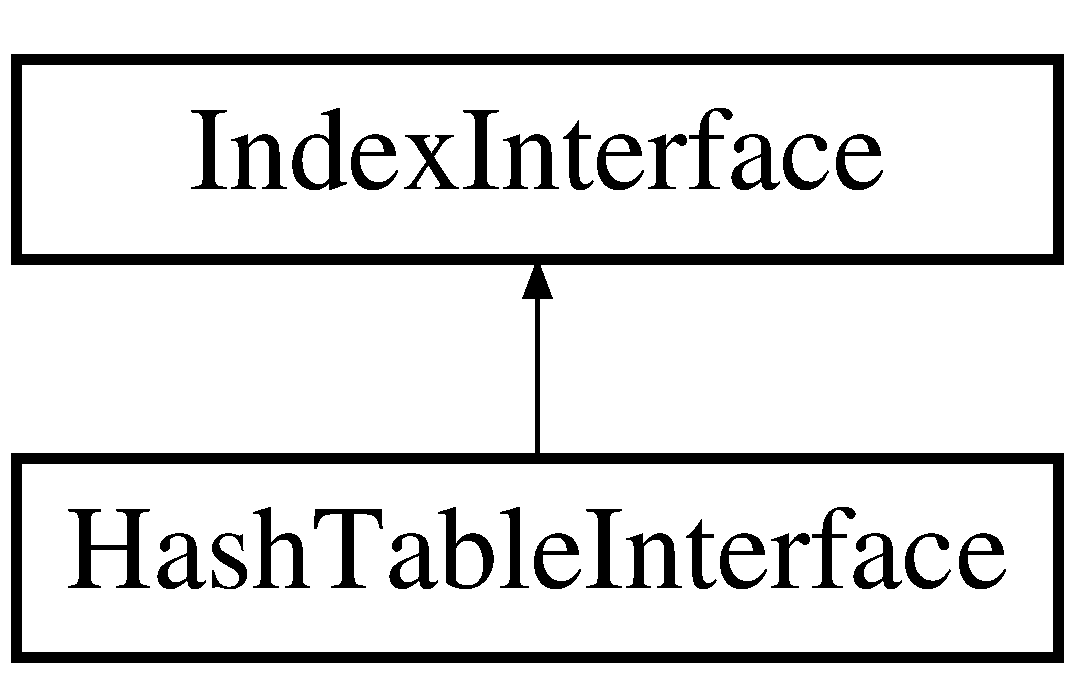
\includegraphics[height=2.000000cm]{class_hash_table_interface}
\end{center}
\end{figure}
\subsection*{Public Member Functions}
\begin{DoxyCompactItemize}
\item 
\hyperlink{class_hash_table_interface_afcc090bbeda66c331a7a28623aad5d0c}{Hash\+Table\+Interface} ()
\item 
\hyperlink{class_hash_table_interface_ab0a34d3f1ee275590002fc4c5d4327fe}{$\sim$\+Hash\+Table\+Interface} ()
\item 
void \hyperlink{class_index_interface_a7f082789ce91eaaacc10a5c841b62cd4}{append\+\_\+page\+\_\+info} (\hyperlink{class_page_info}{Page\+Info} $\ast$curr\+Info)
\item 
double \hyperlink{class_index_interface_a8195aee88cd593c2e6ca2e2c48cbd068}{calc\+\_\+tdidf} (int page\+I\+D, int freq, int spread)
\item 
void \hyperlink{class_index_interface_a7e4d5fe8c31cfc9aa02c2dd1d7e1d3aa}{display\+\_\+result} (int rank, int page\+I\+D, double tdidf)
\item 
void \hyperlink{class_index_interface_a3d784385e028557312ef15d59574f9ed}{display\+\_\+page\+\_\+content} (int page\+I\+D)
\item 
void \hyperlink{class_index_interface_a5734b1488a787d47984bf97ffa5aff8d}{incr\+\_\+total\+\_\+words\+\_\+on\+\_\+page} (int curr\+I\+D, int incr)
\item 
void \hyperlink{class_index_interface_a229f1eb93f38d85d78e64e579c46c98a}{read\+\_\+file} (string file\+Path)
\item 
void \hyperlink{class_index_interface_aebcf89c2fd27b815b697c8e9d29e0c3a}{read\+\_\+persistence\+\_\+files} ()
\item 
void \hyperlink{class_index_interface_a0ca6250b71da3983ca31afdf3ee6dd88}{read\+\_\+pers\+\_\+file} (int index)
\item 
virtual void \hyperlink{class_index_interface_aa83b7083d107869e3519c5862bc71d0a}{add\+\_\+term\+\_\+to\+\_\+ii} (int letter\+Index, \hyperlink{class_term}{Term} $\ast$term)
\item 
virtual void \hyperlink{class_index_interface_ad7b88501f360ccfad0c1ee08d793ca25}{clear} ()
\item 
virtual \hyperlink{class_term}{Term} $\ast$ \hyperlink{class_index_interface_a851f0396f0b390cc9aa8cde270afffc9}{find\+\_\+term} (string term)
\item 
virtual void \hyperlink{class_index_interface_a0b4ec5fcc32c08959cffad3a3141dd4e}{write\+\_\+persistence\+\_\+files} ()
\item 
int \hyperlink{class_index_interface_a9a7539d9c7a48bf4d4fbe43961c0547f}{index\+\_\+for\+\_\+letter} (char letter)
\item 
\hyperlink{class_page_info}{Page\+Info} $\ast$ \hyperlink{class_index_interface_a2af7d88c3b2701be9164ba9f4a3bddb3}{info\+\_\+for\+\_\+page\+I\+D} (int page\+I\+D)
\item 
int \hyperlink{class_index_interface_a8a0132ad6e84c4340061496c615f581c}{get\+\_\+total\+Words\+In\+Corpus} ()
\item 
int \hyperlink{class_index_interface_af9edc24ac00bdf2c0e06384f890a1d8a}{get\+\_\+total\+Pages} ()
\end{DoxyCompactItemize}
\subsection*{Protected Attributes}
\begin{DoxyCompactItemize}
\item 
const string \hyperlink{class_index_interface_acd76893126e9fd5dc63cb4ea8f56265c}{ext} = \char`\"{}.txt\char`\"{}
\item 
\hyperlink{class_hash_table_index}{Hash\+Table\+Index} $\ast$ \hyperlink{class_index_interface_a8511509bb58da989f705ba75fd5dde2d}{letters}
\item 
vector$<$ \hyperlink{class_page_info}{Page\+Info} $\ast$ $>$ \hyperlink{class_index_interface_a8400a62750faa69ff35308ff731d9ee5}{info\+For\+I\+Ds}
\item 
\hyperlink{class_doc_parser}{Doc\+Parser} \& \hyperlink{class_index_interface_a42b0d9eccd309185ed92976f72908bb9}{parser}
\item 
int \hyperlink{class_index_interface_a2df695d2b504f2e53a0bfdd6bfee31da}{total\+Pages}
\item 
int \hyperlink{class_index_interface_ab607b430e78528cdb8bb79ba4afa91d2}{total\+Words\+In\+Corpus}
\end{DoxyCompactItemize}


\subsection{Detailed Description}
\hyperlink{class_hash_table_interface}{Hash\+Table\+Interface} creates hash table index\textquotesingle{}s. 

\subsection{Constructor \& Destructor Documentation}
\hypertarget{class_hash_table_interface_afcc090bbeda66c331a7a28623aad5d0c}{}\index{Hash\+Table\+Interface@{Hash\+Table\+Interface}!Hash\+Table\+Interface@{Hash\+Table\+Interface}}
\index{Hash\+Table\+Interface@{Hash\+Table\+Interface}!Hash\+Table\+Interface@{Hash\+Table\+Interface}}
\subsubsection[{Hash\+Table\+Interface}]{\setlength{\rightskip}{0pt plus 5cm}Hash\+Table\+Interface\+::\+Hash\+Table\+Interface (
\begin{DoxyParamCaption}
{}
\end{DoxyParamCaption}
)}\label{class_hash_table_interface_afcc090bbeda66c331a7a28623aad5d0c}
\hypertarget{class_hash_table_interface_ab0a34d3f1ee275590002fc4c5d4327fe}{}\index{Hash\+Table\+Interface@{Hash\+Table\+Interface}!````~Hash\+Table\+Interface@{$\sim$\+Hash\+Table\+Interface}}
\index{````~Hash\+Table\+Interface@{$\sim$\+Hash\+Table\+Interface}!Hash\+Table\+Interface@{Hash\+Table\+Interface}}
\subsubsection[{$\sim$\+Hash\+Table\+Interface}]{\setlength{\rightskip}{0pt plus 5cm}Hash\+Table\+Interface\+::$\sim$\+Hash\+Table\+Interface (
\begin{DoxyParamCaption}
{}
\end{DoxyParamCaption}
)}\label{class_hash_table_interface_ab0a34d3f1ee275590002fc4c5d4327fe}


\subsection{Member Function Documentation}
\hypertarget{class_index_interface_aa83b7083d107869e3519c5862bc71d0a}{}\index{Hash\+Table\+Interface@{Hash\+Table\+Interface}!add\+\_\+term\+\_\+to\+\_\+ii@{add\+\_\+term\+\_\+to\+\_\+ii}}
\index{add\+\_\+term\+\_\+to\+\_\+ii@{add\+\_\+term\+\_\+to\+\_\+ii}!Hash\+Table\+Interface@{Hash\+Table\+Interface}}
\subsubsection[{add\+\_\+term\+\_\+to\+\_\+ii}]{\setlength{\rightskip}{0pt plus 5cm}void Index\+Interface\+::add\+\_\+term\+\_\+to\+\_\+ii (
\begin{DoxyParamCaption}
\item[{int}]{letter\+Index, }
\item[{{\bf Term} $\ast$}]{term}
\end{DoxyParamCaption}
)\hspace{0.3cm}{\ttfamily [virtual]}, {\ttfamily [inherited]}}\label{class_index_interface_aa83b7083d107869e3519c5862bc71d0a}


Reimplemented in \hyperlink{class_a_v_l_tree_interface_a2ff7466f1fd70ce6391330c04749fec7}{A\+V\+L\+Tree\+Interface}.

\hypertarget{class_index_interface_a7f082789ce91eaaacc10a5c841b62cd4}{}\index{Hash\+Table\+Interface@{Hash\+Table\+Interface}!append\+\_\+page\+\_\+info@{append\+\_\+page\+\_\+info}}
\index{append\+\_\+page\+\_\+info@{append\+\_\+page\+\_\+info}!Hash\+Table\+Interface@{Hash\+Table\+Interface}}
\subsubsection[{append\+\_\+page\+\_\+info}]{\setlength{\rightskip}{0pt plus 5cm}void Index\+Interface\+::append\+\_\+page\+\_\+info (
\begin{DoxyParamCaption}
\item[{{\bf Page\+Info} $\ast$}]{curr\+Info}
\end{DoxyParamCaption}
)\hspace{0.3cm}{\ttfamily [inherited]}}\label{class_index_interface_a7f082789ce91eaaacc10a5c841b62cd4}
\hypertarget{class_index_interface_a8195aee88cd593c2e6ca2e2c48cbd068}{}\index{Hash\+Table\+Interface@{Hash\+Table\+Interface}!calc\+\_\+tdidf@{calc\+\_\+tdidf}}
\index{calc\+\_\+tdidf@{calc\+\_\+tdidf}!Hash\+Table\+Interface@{Hash\+Table\+Interface}}
\subsubsection[{calc\+\_\+tdidf}]{\setlength{\rightskip}{0pt plus 5cm}double Index\+Interface\+::calc\+\_\+tdidf (
\begin{DoxyParamCaption}
\item[{int}]{page\+I\+D, }
\item[{int}]{freq, }
\item[{int}]{spread}
\end{DoxyParamCaption}
)\hspace{0.3cm}{\ttfamily [inherited]}}\label{class_index_interface_a8195aee88cd593c2e6ca2e2c48cbd068}
\hypertarget{class_index_interface_ad7b88501f360ccfad0c1ee08d793ca25}{}\index{Hash\+Table\+Interface@{Hash\+Table\+Interface}!clear@{clear}}
\index{clear@{clear}!Hash\+Table\+Interface@{Hash\+Table\+Interface}}
\subsubsection[{clear}]{\setlength{\rightskip}{0pt plus 5cm}void Index\+Interface\+::clear (
\begin{DoxyParamCaption}
{}
\end{DoxyParamCaption}
)\hspace{0.3cm}{\ttfamily [virtual]}, {\ttfamily [inherited]}}\label{class_index_interface_ad7b88501f360ccfad0c1ee08d793ca25}


Reimplemented in \hyperlink{class_a_v_l_tree_interface_a748ffc895fb64aab3e2afac287f80630}{A\+V\+L\+Tree\+Interface}.

\hypertarget{class_index_interface_a3d784385e028557312ef15d59574f9ed}{}\index{Hash\+Table\+Interface@{Hash\+Table\+Interface}!display\+\_\+page\+\_\+content@{display\+\_\+page\+\_\+content}}
\index{display\+\_\+page\+\_\+content@{display\+\_\+page\+\_\+content}!Hash\+Table\+Interface@{Hash\+Table\+Interface}}
\subsubsection[{display\+\_\+page\+\_\+content}]{\setlength{\rightskip}{0pt plus 5cm}void Index\+Interface\+::display\+\_\+page\+\_\+content (
\begin{DoxyParamCaption}
\item[{int}]{page\+I\+D}
\end{DoxyParamCaption}
)\hspace{0.3cm}{\ttfamily [inherited]}}\label{class_index_interface_a3d784385e028557312ef15d59574f9ed}
\hypertarget{class_index_interface_a7e4d5fe8c31cfc9aa02c2dd1d7e1d3aa}{}\index{Hash\+Table\+Interface@{Hash\+Table\+Interface}!display\+\_\+result@{display\+\_\+result}}
\index{display\+\_\+result@{display\+\_\+result}!Hash\+Table\+Interface@{Hash\+Table\+Interface}}
\subsubsection[{display\+\_\+result}]{\setlength{\rightskip}{0pt plus 5cm}void Index\+Interface\+::display\+\_\+result (
\begin{DoxyParamCaption}
\item[{int}]{rank, }
\item[{int}]{page\+I\+D, }
\item[{double}]{tdidf}
\end{DoxyParamCaption}
)\hspace{0.3cm}{\ttfamily [inherited]}}\label{class_index_interface_a7e4d5fe8c31cfc9aa02c2dd1d7e1d3aa}
\hypertarget{class_index_interface_a851f0396f0b390cc9aa8cde270afffc9}{}\index{Hash\+Table\+Interface@{Hash\+Table\+Interface}!find\+\_\+term@{find\+\_\+term}}
\index{find\+\_\+term@{find\+\_\+term}!Hash\+Table\+Interface@{Hash\+Table\+Interface}}
\subsubsection[{find\+\_\+term}]{\setlength{\rightskip}{0pt plus 5cm}{\bf Term} $\ast$ Index\+Interface\+::find\+\_\+term (
\begin{DoxyParamCaption}
\item[{string}]{term}
\end{DoxyParamCaption}
)\hspace{0.3cm}{\ttfamily [virtual]}, {\ttfamily [inherited]}}\label{class_index_interface_a851f0396f0b390cc9aa8cde270afffc9}


Reimplemented in \hyperlink{class_a_v_l_tree_interface_a35ee941b125e65cf0b5783a687503d83}{A\+V\+L\+Tree\+Interface}.

\hypertarget{class_index_interface_af9edc24ac00bdf2c0e06384f890a1d8a}{}\index{Hash\+Table\+Interface@{Hash\+Table\+Interface}!get\+\_\+total\+Pages@{get\+\_\+total\+Pages}}
\index{get\+\_\+total\+Pages@{get\+\_\+total\+Pages}!Hash\+Table\+Interface@{Hash\+Table\+Interface}}
\subsubsection[{get\+\_\+total\+Pages}]{\setlength{\rightskip}{0pt plus 5cm}int Index\+Interface\+::get\+\_\+total\+Pages (
\begin{DoxyParamCaption}
{}
\end{DoxyParamCaption}
)\hspace{0.3cm}{\ttfamily [inherited]}}\label{class_index_interface_af9edc24ac00bdf2c0e06384f890a1d8a}
\hypertarget{class_index_interface_a8a0132ad6e84c4340061496c615f581c}{}\index{Hash\+Table\+Interface@{Hash\+Table\+Interface}!get\+\_\+total\+Words\+In\+Corpus@{get\+\_\+total\+Words\+In\+Corpus}}
\index{get\+\_\+total\+Words\+In\+Corpus@{get\+\_\+total\+Words\+In\+Corpus}!Hash\+Table\+Interface@{Hash\+Table\+Interface}}
\subsubsection[{get\+\_\+total\+Words\+In\+Corpus}]{\setlength{\rightskip}{0pt plus 5cm}int Index\+Interface\+::get\+\_\+total\+Words\+In\+Corpus (
\begin{DoxyParamCaption}
{}
\end{DoxyParamCaption}
)\hspace{0.3cm}{\ttfamily [inherited]}}\label{class_index_interface_a8a0132ad6e84c4340061496c615f581c}
\hypertarget{class_index_interface_a5734b1488a787d47984bf97ffa5aff8d}{}\index{Hash\+Table\+Interface@{Hash\+Table\+Interface}!incr\+\_\+total\+\_\+words\+\_\+on\+\_\+page@{incr\+\_\+total\+\_\+words\+\_\+on\+\_\+page}}
\index{incr\+\_\+total\+\_\+words\+\_\+on\+\_\+page@{incr\+\_\+total\+\_\+words\+\_\+on\+\_\+page}!Hash\+Table\+Interface@{Hash\+Table\+Interface}}
\subsubsection[{incr\+\_\+total\+\_\+words\+\_\+on\+\_\+page}]{\setlength{\rightskip}{0pt plus 5cm}void Index\+Interface\+::incr\+\_\+total\+\_\+words\+\_\+on\+\_\+page (
\begin{DoxyParamCaption}
\item[{int}]{curr\+I\+D, }
\item[{int}]{incr}
\end{DoxyParamCaption}
)\hspace{0.3cm}{\ttfamily [inherited]}}\label{class_index_interface_a5734b1488a787d47984bf97ffa5aff8d}
\hypertarget{class_index_interface_a9a7539d9c7a48bf4d4fbe43961c0547f}{}\index{Hash\+Table\+Interface@{Hash\+Table\+Interface}!index\+\_\+for\+\_\+letter@{index\+\_\+for\+\_\+letter}}
\index{index\+\_\+for\+\_\+letter@{index\+\_\+for\+\_\+letter}!Hash\+Table\+Interface@{Hash\+Table\+Interface}}
\subsubsection[{index\+\_\+for\+\_\+letter}]{\setlength{\rightskip}{0pt plus 5cm}int Index\+Interface\+::index\+\_\+for\+\_\+letter (
\begin{DoxyParamCaption}
\item[{char}]{letter}
\end{DoxyParamCaption}
)\hspace{0.3cm}{\ttfamily [inherited]}}\label{class_index_interface_a9a7539d9c7a48bf4d4fbe43961c0547f}
\hypertarget{class_index_interface_a2af7d88c3b2701be9164ba9f4a3bddb3}{}\index{Hash\+Table\+Interface@{Hash\+Table\+Interface}!info\+\_\+for\+\_\+page\+I\+D@{info\+\_\+for\+\_\+page\+I\+D}}
\index{info\+\_\+for\+\_\+page\+I\+D@{info\+\_\+for\+\_\+page\+I\+D}!Hash\+Table\+Interface@{Hash\+Table\+Interface}}
\subsubsection[{info\+\_\+for\+\_\+page\+I\+D}]{\setlength{\rightskip}{0pt plus 5cm}{\bf Page\+Info} $\ast$ Index\+Interface\+::info\+\_\+for\+\_\+page\+I\+D (
\begin{DoxyParamCaption}
\item[{int}]{page\+I\+D}
\end{DoxyParamCaption}
)\hspace{0.3cm}{\ttfamily [inherited]}}\label{class_index_interface_a2af7d88c3b2701be9164ba9f4a3bddb3}
\hypertarget{class_index_interface_a229f1eb93f38d85d78e64e579c46c98a}{}\index{Hash\+Table\+Interface@{Hash\+Table\+Interface}!read\+\_\+file@{read\+\_\+file}}
\index{read\+\_\+file@{read\+\_\+file}!Hash\+Table\+Interface@{Hash\+Table\+Interface}}
\subsubsection[{read\+\_\+file}]{\setlength{\rightskip}{0pt plus 5cm}void Index\+Interface\+::read\+\_\+file (
\begin{DoxyParamCaption}
\item[{string}]{file\+Path}
\end{DoxyParamCaption}
)\hspace{0.3cm}{\ttfamily [inherited]}}\label{class_index_interface_a229f1eb93f38d85d78e64e579c46c98a}
\hypertarget{class_index_interface_a0ca6250b71da3983ca31afdf3ee6dd88}{}\index{Hash\+Table\+Interface@{Hash\+Table\+Interface}!read\+\_\+pers\+\_\+file@{read\+\_\+pers\+\_\+file}}
\index{read\+\_\+pers\+\_\+file@{read\+\_\+pers\+\_\+file}!Hash\+Table\+Interface@{Hash\+Table\+Interface}}
\subsubsection[{read\+\_\+pers\+\_\+file}]{\setlength{\rightskip}{0pt plus 5cm}void Index\+Interface\+::read\+\_\+pers\+\_\+file (
\begin{DoxyParamCaption}
\item[{int}]{index}
\end{DoxyParamCaption}
)\hspace{0.3cm}{\ttfamily [inherited]}}\label{class_index_interface_a0ca6250b71da3983ca31afdf3ee6dd88}
\hypertarget{class_index_interface_aebcf89c2fd27b815b697c8e9d29e0c3a}{}\index{Hash\+Table\+Interface@{Hash\+Table\+Interface}!read\+\_\+persistence\+\_\+files@{read\+\_\+persistence\+\_\+files}}
\index{read\+\_\+persistence\+\_\+files@{read\+\_\+persistence\+\_\+files}!Hash\+Table\+Interface@{Hash\+Table\+Interface}}
\subsubsection[{read\+\_\+persistence\+\_\+files}]{\setlength{\rightskip}{0pt plus 5cm}void Index\+Interface\+::read\+\_\+persistence\+\_\+files (
\begin{DoxyParamCaption}
{}
\end{DoxyParamCaption}
)\hspace{0.3cm}{\ttfamily [inherited]}}\label{class_index_interface_aebcf89c2fd27b815b697c8e9d29e0c3a}
\hypertarget{class_index_interface_a0b4ec5fcc32c08959cffad3a3141dd4e}{}\index{Hash\+Table\+Interface@{Hash\+Table\+Interface}!write\+\_\+persistence\+\_\+files@{write\+\_\+persistence\+\_\+files}}
\index{write\+\_\+persistence\+\_\+files@{write\+\_\+persistence\+\_\+files}!Hash\+Table\+Interface@{Hash\+Table\+Interface}}
\subsubsection[{write\+\_\+persistence\+\_\+files}]{\setlength{\rightskip}{0pt plus 5cm}void Index\+Interface\+::write\+\_\+persistence\+\_\+files (
\begin{DoxyParamCaption}
{}
\end{DoxyParamCaption}
)\hspace{0.3cm}{\ttfamily [virtual]}, {\ttfamily [inherited]}}\label{class_index_interface_a0b4ec5fcc32c08959cffad3a3141dd4e}


Reimplemented in \hyperlink{class_a_v_l_tree_interface_abd7f70746611a3982dc07a1b1880e7b5}{A\+V\+L\+Tree\+Interface}.



\subsection{Member Data Documentation}
\hypertarget{class_index_interface_acd76893126e9fd5dc63cb4ea8f56265c}{}\index{Hash\+Table\+Interface@{Hash\+Table\+Interface}!ext@{ext}}
\index{ext@{ext}!Hash\+Table\+Interface@{Hash\+Table\+Interface}}
\subsubsection[{ext}]{\setlength{\rightskip}{0pt plus 5cm}const string Index\+Interface\+::ext = \char`\"{}.txt\char`\"{}\hspace{0.3cm}{\ttfamily [protected]}, {\ttfamily [inherited]}}\label{class_index_interface_acd76893126e9fd5dc63cb4ea8f56265c}
\hypertarget{class_index_interface_a8400a62750faa69ff35308ff731d9ee5}{}\index{Hash\+Table\+Interface@{Hash\+Table\+Interface}!info\+For\+I\+Ds@{info\+For\+I\+Ds}}
\index{info\+For\+I\+Ds@{info\+For\+I\+Ds}!Hash\+Table\+Interface@{Hash\+Table\+Interface}}
\subsubsection[{info\+For\+I\+Ds}]{\setlength{\rightskip}{0pt plus 5cm}vector$<${\bf Page\+Info}$\ast$$>$ Index\+Interface\+::info\+For\+I\+Ds\hspace{0.3cm}{\ttfamily [protected]}, {\ttfamily [inherited]}}\label{class_index_interface_a8400a62750faa69ff35308ff731d9ee5}
\hypertarget{class_index_interface_a8511509bb58da989f705ba75fd5dde2d}{}\index{Hash\+Table\+Interface@{Hash\+Table\+Interface}!letters@{letters}}
\index{letters@{letters}!Hash\+Table\+Interface@{Hash\+Table\+Interface}}
\subsubsection[{letters}]{\setlength{\rightskip}{0pt plus 5cm}{\bf Hash\+Table\+Index}$\ast$ Index\+Interface\+::letters\hspace{0.3cm}{\ttfamily [protected]}, {\ttfamily [inherited]}}\label{class_index_interface_a8511509bb58da989f705ba75fd5dde2d}
\hypertarget{class_index_interface_a42b0d9eccd309185ed92976f72908bb9}{}\index{Hash\+Table\+Interface@{Hash\+Table\+Interface}!parser@{parser}}
\index{parser@{parser}!Hash\+Table\+Interface@{Hash\+Table\+Interface}}
\subsubsection[{parser}]{\setlength{\rightskip}{0pt plus 5cm}{\bf Doc\+Parser}\& Index\+Interface\+::parser\hspace{0.3cm}{\ttfamily [protected]}, {\ttfamily [inherited]}}\label{class_index_interface_a42b0d9eccd309185ed92976f72908bb9}
\hypertarget{class_index_interface_a2df695d2b504f2e53a0bfdd6bfee31da}{}\index{Hash\+Table\+Interface@{Hash\+Table\+Interface}!total\+Pages@{total\+Pages}}
\index{total\+Pages@{total\+Pages}!Hash\+Table\+Interface@{Hash\+Table\+Interface}}
\subsubsection[{total\+Pages}]{\setlength{\rightskip}{0pt plus 5cm}int Index\+Interface\+::total\+Pages\hspace{0.3cm}{\ttfamily [protected]}, {\ttfamily [inherited]}}\label{class_index_interface_a2df695d2b504f2e53a0bfdd6bfee31da}
\hypertarget{class_index_interface_ab607b430e78528cdb8bb79ba4afa91d2}{}\index{Hash\+Table\+Interface@{Hash\+Table\+Interface}!total\+Words\+In\+Corpus@{total\+Words\+In\+Corpus}}
\index{total\+Words\+In\+Corpus@{total\+Words\+In\+Corpus}!Hash\+Table\+Interface@{Hash\+Table\+Interface}}
\subsubsection[{total\+Words\+In\+Corpus}]{\setlength{\rightskip}{0pt plus 5cm}int Index\+Interface\+::total\+Words\+In\+Corpus\hspace{0.3cm}{\ttfamily [protected]}, {\ttfamily [inherited]}}\label{class_index_interface_ab607b430e78528cdb8bb79ba4afa91d2}


The documentation for this class was generated from the following files\+:\begin{DoxyCompactItemize}
\item 
\hyperlink{hashtableinterface_8h}{hashtableinterface.\+h}\item 
\hyperlink{hashtableinterface_8cpp}{hashtableinterface.\+cpp}\end{DoxyCompactItemize}

\hypertarget{structrapidxml_1_1memory__pool_1_1header}{}\section{rapidxml\+:\+:memory\+\_\+pool$<$ Ch $>$\+:\+:header Struct Reference}
\label{structrapidxml_1_1memory__pool_1_1header}\index{rapidxml\+::memory\+\_\+pool$<$ Ch $>$\+::header@{rapidxml\+::memory\+\_\+pool$<$ Ch $>$\+::header}}
\subsection*{Public Attributes}
\begin{DoxyCompactItemize}
\item 
char $\ast$ \hyperlink{structrapidxml_1_1memory__pool_1_1header_a3035f6741bb38f91c7f2efd05398c23d}{previous\+\_\+begin}
\end{DoxyCompactItemize}


\subsection{Member Data Documentation}
\hypertarget{structrapidxml_1_1memory__pool_1_1header_a3035f6741bb38f91c7f2efd05398c23d}{}\index{rapidxml\+::memory\+\_\+pool\+::header@{rapidxml\+::memory\+\_\+pool\+::header}!previous\+\_\+begin@{previous\+\_\+begin}}
\index{previous\+\_\+begin@{previous\+\_\+begin}!rapidxml\+::memory\+\_\+pool\+::header@{rapidxml\+::memory\+\_\+pool\+::header}}
\subsubsection[{previous\+\_\+begin}]{\setlength{\rightskip}{0pt plus 5cm}template$<$class Ch  = char$>$ char$\ast$ {\bf rapidxml\+::memory\+\_\+pool}$<$ Ch $>$\+::header\+::previous\+\_\+begin}\label{structrapidxml_1_1memory__pool_1_1header_a3035f6741bb38f91c7f2efd05398c23d}


The documentation for this struct was generated from the following file\+:\begin{DoxyCompactItemize}
\item 
\hyperlink{rapidxml_8hpp}{rapidxml.\+hpp}\end{DoxyCompactItemize}

\hypertarget{class_index_handler}{}\section{Index\+Handler Class Reference}
\label{class_index_handler}\index{Index\+Handler@{Index\+Handler}}


{\ttfamily \#include $<$indexhandler.\+h$>$}

\subsection*{Public Member Functions}
\begin{DoxyCompactItemize}
\item 
\hyperlink{class_index_handler_a27748387661142a2eb545be6f0499996}{Index\+Handler} ()
\item 
\hyperlink{class_index_handler_ad787ca8cf83345ecfe332d2c3b8f8009}{$\sim$\+Index\+Handler} ()
\item 
\hyperlink{class_index_handler_ae50be3bec7e5ad3ede66110535043e15}{Index\+Handler} (bool as\+Hash\+Table)
\item 
void \hyperlink{class_index_handler_a3fe9b3c1b3df7eea7e4ae590df4a4339}{read\+\_\+file} (string file\+Path)
\item 
void \hyperlink{class_index_handler_acee974285412a635c3c31fe86b9e0fb8}{run\+\_\+queries} (string query)
\item 
void \hyperlink{class_index_handler_a417830272cfc725f6966c7a0a0ceae1d}{clear\+\_\+index} ()
\end{DoxyCompactItemize}
\subsection*{Private Attributes}
\begin{DoxyCompactItemize}
\item 
\hyperlink{class_index_interface}{Index\+Interface} $\ast$ \hyperlink{class_index_handler_aa30663ff8e3b52b43ce35ebb2d12752c}{index}
\end{DoxyCompactItemize}


\subsection{Constructor \& Destructor Documentation}
\hypertarget{class_index_handler_a27748387661142a2eb545be6f0499996}{}\index{Index\+Handler@{Index\+Handler}!Index\+Handler@{Index\+Handler}}
\index{Index\+Handler@{Index\+Handler}!Index\+Handler@{Index\+Handler}}
\subsubsection[{Index\+Handler}]{\setlength{\rightskip}{0pt plus 5cm}Index\+Handler\+::\+Index\+Handler (
\begin{DoxyParamCaption}
{}
\end{DoxyParamCaption}
)}\label{class_index_handler_a27748387661142a2eb545be6f0499996}
\hypertarget{class_index_handler_ad787ca8cf83345ecfe332d2c3b8f8009}{}\index{Index\+Handler@{Index\+Handler}!````~Index\+Handler@{$\sim$\+Index\+Handler}}
\index{````~Index\+Handler@{$\sim$\+Index\+Handler}!Index\+Handler@{Index\+Handler}}
\subsubsection[{$\sim$\+Index\+Handler}]{\setlength{\rightskip}{0pt plus 5cm}Index\+Handler\+::$\sim$\+Index\+Handler (
\begin{DoxyParamCaption}
{}
\end{DoxyParamCaption}
)}\label{class_index_handler_ad787ca8cf83345ecfe332d2c3b8f8009}
\hypertarget{class_index_handler_ae50be3bec7e5ad3ede66110535043e15}{}\index{Index\+Handler@{Index\+Handler}!Index\+Handler@{Index\+Handler}}
\index{Index\+Handler@{Index\+Handler}!Index\+Handler@{Index\+Handler}}
\subsubsection[{Index\+Handler}]{\setlength{\rightskip}{0pt plus 5cm}Index\+Handler\+::\+Index\+Handler (
\begin{DoxyParamCaption}
\item[{bool}]{as\+Hash\+Table}
\end{DoxyParamCaption}
)}\label{class_index_handler_ae50be3bec7e5ad3ede66110535043e15}


\subsection{Member Function Documentation}
\hypertarget{class_index_handler_a417830272cfc725f6966c7a0a0ceae1d}{}\index{Index\+Handler@{Index\+Handler}!clear\+\_\+index@{clear\+\_\+index}}
\index{clear\+\_\+index@{clear\+\_\+index}!Index\+Handler@{Index\+Handler}}
\subsubsection[{clear\+\_\+index}]{\setlength{\rightskip}{0pt plus 5cm}void Index\+Handler\+::clear\+\_\+index (
\begin{DoxyParamCaption}
{}
\end{DoxyParamCaption}
)}\label{class_index_handler_a417830272cfc725f6966c7a0a0ceae1d}
\hypertarget{class_index_handler_a3fe9b3c1b3df7eea7e4ae590df4a4339}{}\index{Index\+Handler@{Index\+Handler}!read\+\_\+file@{read\+\_\+file}}
\index{read\+\_\+file@{read\+\_\+file}!Index\+Handler@{Index\+Handler}}
\subsubsection[{read\+\_\+file}]{\setlength{\rightskip}{0pt plus 5cm}void Index\+Handler\+::read\+\_\+file (
\begin{DoxyParamCaption}
\item[{string}]{file\+Path}
\end{DoxyParamCaption}
)}\label{class_index_handler_a3fe9b3c1b3df7eea7e4ae590df4a4339}
\hypertarget{class_index_handler_acee974285412a635c3c31fe86b9e0fb8}{}\index{Index\+Handler@{Index\+Handler}!run\+\_\+queries@{run\+\_\+queries}}
\index{run\+\_\+queries@{run\+\_\+queries}!Index\+Handler@{Index\+Handler}}
\subsubsection[{run\+\_\+queries}]{\setlength{\rightskip}{0pt plus 5cm}void Index\+Handler\+::run\+\_\+queries (
\begin{DoxyParamCaption}
\item[{string}]{query}
\end{DoxyParamCaption}
)}\label{class_index_handler_acee974285412a635c3c31fe86b9e0fb8}


\subsection{Member Data Documentation}
\hypertarget{class_index_handler_aa30663ff8e3b52b43ce35ebb2d12752c}{}\index{Index\+Handler@{Index\+Handler}!index@{index}}
\index{index@{index}!Index\+Handler@{Index\+Handler}}
\subsubsection[{index}]{\setlength{\rightskip}{0pt plus 5cm}{\bf Index\+Interface}$\ast$ Index\+Handler\+::index\hspace{0.3cm}{\ttfamily [private]}}\label{class_index_handler_aa30663ff8e3b52b43ce35ebb2d12752c}


The documentation for this class was generated from the following files\+:\begin{DoxyCompactItemize}
\item 
\hyperlink{indexhandler_8h}{indexhandler.\+h}\item 
\hyperlink{indexhandler_8cpp}{indexhandler.\+cpp}\end{DoxyCompactItemize}

\hypertarget{class_index_interface}{}\section{Index\+Interface Class Reference}
\label{class_index_interface}\index{Index\+Interface@{Index\+Interface}}


A\+V\+L Node implementation for the A\+V\+L Tree structure.  




{\ttfamily \#include $<$indexinterface.\+h$>$}

Inheritance diagram for Index\+Interface\+:\begin{figure}[H]
\begin{center}
\leavevmode
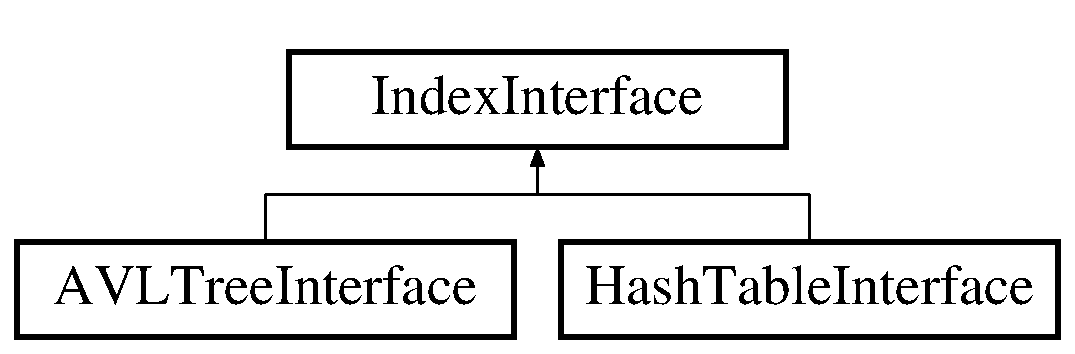
\includegraphics[height=2.000000cm]{class_index_interface}
\end{center}
\end{figure}
\subsection*{Public Member Functions}
\begin{DoxyCompactItemize}
\item 
\hyperlink{class_index_interface_a7b1e7eae7faa652d2f63efeecf0ca2de}{Index\+Interface} ()
\item 
\hyperlink{class_index_interface_a3927fabe77a7da5845dc0495b2c1c2b2}{$\sim$\+Index\+Interface} ()
\item 
void \hyperlink{class_index_interface_a7f082789ce91eaaacc10a5c841b62cd4}{append\+\_\+page\+\_\+info} (\hyperlink{class_page_info}{Page\+Info} $\ast$curr\+Info)
\item 
double \hyperlink{class_index_interface_a8195aee88cd593c2e6ca2e2c48cbd068}{calc\+\_\+tdidf} (int page\+I\+D, int freq, int spread)
\item 
void \hyperlink{class_index_interface_a7e4d5fe8c31cfc9aa02c2dd1d7e1d3aa}{display\+\_\+result} (int rank, int page\+I\+D, double tdidf)
\item 
void \hyperlink{class_index_interface_a3d784385e028557312ef15d59574f9ed}{display\+\_\+page\+\_\+content} (int page\+I\+D)
\item 
void \hyperlink{class_index_interface_a5734b1488a787d47984bf97ffa5aff8d}{incr\+\_\+total\+\_\+words\+\_\+on\+\_\+page} (int curr\+I\+D, int incr)
\item 
void \hyperlink{class_index_interface_a229f1eb93f38d85d78e64e579c46c98a}{read\+\_\+file} (string file\+Path)
\item 
void \hyperlink{class_index_interface_aebcf89c2fd27b815b697c8e9d29e0c3a}{read\+\_\+persistence\+\_\+files} ()
\item 
void \hyperlink{class_index_interface_a0ca6250b71da3983ca31afdf3ee6dd88}{read\+\_\+pers\+\_\+file} (int index)
\item 
virtual void \hyperlink{class_index_interface_aa83b7083d107869e3519c5862bc71d0a}{add\+\_\+term\+\_\+to\+\_\+ii} (int letter\+Index, \hyperlink{class_term}{Term} $\ast$term)
\item 
virtual void \hyperlink{class_index_interface_ad7b88501f360ccfad0c1ee08d793ca25}{clear} ()
\item 
virtual \hyperlink{class_term}{Term} $\ast$ \hyperlink{class_index_interface_a851f0396f0b390cc9aa8cde270afffc9}{find\+\_\+term} (string term)
\item 
virtual void \hyperlink{class_index_interface_a0b4ec5fcc32c08959cffad3a3141dd4e}{write\+\_\+persistence\+\_\+files} ()
\item 
int \hyperlink{class_index_interface_a9a7539d9c7a48bf4d4fbe43961c0547f}{index\+\_\+for\+\_\+letter} (char letter)
\item 
\hyperlink{class_page_info}{Page\+Info} $\ast$ \hyperlink{class_index_interface_a2af7d88c3b2701be9164ba9f4a3bddb3}{info\+\_\+for\+\_\+page\+I\+D} (int page\+I\+D)
\item 
int \hyperlink{class_index_interface_a8a0132ad6e84c4340061496c615f581c}{get\+\_\+total\+Words\+In\+Corpus} ()
\item 
int \hyperlink{class_index_interface_af9edc24ac00bdf2c0e06384f890a1d8a}{get\+\_\+total\+Pages} ()
\end{DoxyCompactItemize}
\subsection*{Protected Attributes}
\begin{DoxyCompactItemize}
\item 
const string \hyperlink{class_index_interface_acd76893126e9fd5dc63cb4ea8f56265c}{ext} = \char`\"{}.txt\char`\"{}
\item 
\hyperlink{class_hash_table_index}{Hash\+Table\+Index} $\ast$ \hyperlink{class_index_interface_a8511509bb58da989f705ba75fd5dde2d}{letters}
\item 
vector$<$ \hyperlink{class_page_info}{Page\+Info} $\ast$ $>$ \hyperlink{class_index_interface_a8400a62750faa69ff35308ff731d9ee5}{info\+For\+I\+Ds}
\item 
\hyperlink{class_doc_parser}{Doc\+Parser} \& \hyperlink{class_index_interface_a42b0d9eccd309185ed92976f72908bb9}{parser}
\item 
int \hyperlink{class_index_interface_a2df695d2b504f2e53a0bfdd6bfee31da}{total\+Pages}
\item 
int \hyperlink{class_index_interface_ab607b430e78528cdb8bb79ba4afa91d2}{total\+Words\+In\+Corpus}
\end{DoxyCompactItemize}


\subsection{Detailed Description}
A\+V\+L Node implementation for the A\+V\+L Tree structure. 

\subsection{Constructor \& Destructor Documentation}
\hypertarget{class_index_interface_a7b1e7eae7faa652d2f63efeecf0ca2de}{}\index{Index\+Interface@{Index\+Interface}!Index\+Interface@{Index\+Interface}}
\index{Index\+Interface@{Index\+Interface}!Index\+Interface@{Index\+Interface}}
\subsubsection[{Index\+Interface}]{\setlength{\rightskip}{0pt plus 5cm}Index\+Interface\+::\+Index\+Interface (
\begin{DoxyParamCaption}
{}
\end{DoxyParamCaption}
)}\label{class_index_interface_a7b1e7eae7faa652d2f63efeecf0ca2de}
\hypertarget{class_index_interface_a3927fabe77a7da5845dc0495b2c1c2b2}{}\index{Index\+Interface@{Index\+Interface}!````~Index\+Interface@{$\sim$\+Index\+Interface}}
\index{````~Index\+Interface@{$\sim$\+Index\+Interface}!Index\+Interface@{Index\+Interface}}
\subsubsection[{$\sim$\+Index\+Interface}]{\setlength{\rightskip}{0pt plus 5cm}Index\+Interface\+::$\sim$\+Index\+Interface (
\begin{DoxyParamCaption}
{}
\end{DoxyParamCaption}
)}\label{class_index_interface_a3927fabe77a7da5845dc0495b2c1c2b2}


\subsection{Member Function Documentation}
\hypertarget{class_index_interface_aa83b7083d107869e3519c5862bc71d0a}{}\index{Index\+Interface@{Index\+Interface}!add\+\_\+term\+\_\+to\+\_\+ii@{add\+\_\+term\+\_\+to\+\_\+ii}}
\index{add\+\_\+term\+\_\+to\+\_\+ii@{add\+\_\+term\+\_\+to\+\_\+ii}!Index\+Interface@{Index\+Interface}}
\subsubsection[{add\+\_\+term\+\_\+to\+\_\+ii}]{\setlength{\rightskip}{0pt plus 5cm}void Index\+Interface\+::add\+\_\+term\+\_\+to\+\_\+ii (
\begin{DoxyParamCaption}
\item[{int}]{letter\+Index, }
\item[{{\bf Term} $\ast$}]{term}
\end{DoxyParamCaption}
)\hspace{0.3cm}{\ttfamily [virtual]}}\label{class_index_interface_aa83b7083d107869e3519c5862bc71d0a}


Reimplemented in \hyperlink{class_a_v_l_tree_interface_a2ff7466f1fd70ce6391330c04749fec7}{A\+V\+L\+Tree\+Interface}.

\hypertarget{class_index_interface_a7f082789ce91eaaacc10a5c841b62cd4}{}\index{Index\+Interface@{Index\+Interface}!append\+\_\+page\+\_\+info@{append\+\_\+page\+\_\+info}}
\index{append\+\_\+page\+\_\+info@{append\+\_\+page\+\_\+info}!Index\+Interface@{Index\+Interface}}
\subsubsection[{append\+\_\+page\+\_\+info}]{\setlength{\rightskip}{0pt plus 5cm}void Index\+Interface\+::append\+\_\+page\+\_\+info (
\begin{DoxyParamCaption}
\item[{{\bf Page\+Info} $\ast$}]{curr\+Info}
\end{DoxyParamCaption}
)}\label{class_index_interface_a7f082789ce91eaaacc10a5c841b62cd4}
\hypertarget{class_index_interface_a8195aee88cd593c2e6ca2e2c48cbd068}{}\index{Index\+Interface@{Index\+Interface}!calc\+\_\+tdidf@{calc\+\_\+tdidf}}
\index{calc\+\_\+tdidf@{calc\+\_\+tdidf}!Index\+Interface@{Index\+Interface}}
\subsubsection[{calc\+\_\+tdidf}]{\setlength{\rightskip}{0pt plus 5cm}double Index\+Interface\+::calc\+\_\+tdidf (
\begin{DoxyParamCaption}
\item[{int}]{page\+I\+D, }
\item[{int}]{freq, }
\item[{int}]{spread}
\end{DoxyParamCaption}
)}\label{class_index_interface_a8195aee88cd593c2e6ca2e2c48cbd068}
\hypertarget{class_index_interface_ad7b88501f360ccfad0c1ee08d793ca25}{}\index{Index\+Interface@{Index\+Interface}!clear@{clear}}
\index{clear@{clear}!Index\+Interface@{Index\+Interface}}
\subsubsection[{clear}]{\setlength{\rightskip}{0pt plus 5cm}void Index\+Interface\+::clear (
\begin{DoxyParamCaption}
{}
\end{DoxyParamCaption}
)\hspace{0.3cm}{\ttfamily [virtual]}}\label{class_index_interface_ad7b88501f360ccfad0c1ee08d793ca25}


Reimplemented in \hyperlink{class_a_v_l_tree_interface_a748ffc895fb64aab3e2afac287f80630}{A\+V\+L\+Tree\+Interface}.

\hypertarget{class_index_interface_a3d784385e028557312ef15d59574f9ed}{}\index{Index\+Interface@{Index\+Interface}!display\+\_\+page\+\_\+content@{display\+\_\+page\+\_\+content}}
\index{display\+\_\+page\+\_\+content@{display\+\_\+page\+\_\+content}!Index\+Interface@{Index\+Interface}}
\subsubsection[{display\+\_\+page\+\_\+content}]{\setlength{\rightskip}{0pt plus 5cm}void Index\+Interface\+::display\+\_\+page\+\_\+content (
\begin{DoxyParamCaption}
\item[{int}]{page\+I\+D}
\end{DoxyParamCaption}
)}\label{class_index_interface_a3d784385e028557312ef15d59574f9ed}
\hypertarget{class_index_interface_a7e4d5fe8c31cfc9aa02c2dd1d7e1d3aa}{}\index{Index\+Interface@{Index\+Interface}!display\+\_\+result@{display\+\_\+result}}
\index{display\+\_\+result@{display\+\_\+result}!Index\+Interface@{Index\+Interface}}
\subsubsection[{display\+\_\+result}]{\setlength{\rightskip}{0pt plus 5cm}void Index\+Interface\+::display\+\_\+result (
\begin{DoxyParamCaption}
\item[{int}]{rank, }
\item[{int}]{page\+I\+D, }
\item[{double}]{tdidf}
\end{DoxyParamCaption}
)}\label{class_index_interface_a7e4d5fe8c31cfc9aa02c2dd1d7e1d3aa}
\hypertarget{class_index_interface_a851f0396f0b390cc9aa8cde270afffc9}{}\index{Index\+Interface@{Index\+Interface}!find\+\_\+term@{find\+\_\+term}}
\index{find\+\_\+term@{find\+\_\+term}!Index\+Interface@{Index\+Interface}}
\subsubsection[{find\+\_\+term}]{\setlength{\rightskip}{0pt plus 5cm}{\bf Term} $\ast$ Index\+Interface\+::find\+\_\+term (
\begin{DoxyParamCaption}
\item[{string}]{term}
\end{DoxyParamCaption}
)\hspace{0.3cm}{\ttfamily [virtual]}}\label{class_index_interface_a851f0396f0b390cc9aa8cde270afffc9}


Reimplemented in \hyperlink{class_a_v_l_tree_interface_a35ee941b125e65cf0b5783a687503d83}{A\+V\+L\+Tree\+Interface}.

\hypertarget{class_index_interface_af9edc24ac00bdf2c0e06384f890a1d8a}{}\index{Index\+Interface@{Index\+Interface}!get\+\_\+total\+Pages@{get\+\_\+total\+Pages}}
\index{get\+\_\+total\+Pages@{get\+\_\+total\+Pages}!Index\+Interface@{Index\+Interface}}
\subsubsection[{get\+\_\+total\+Pages}]{\setlength{\rightskip}{0pt plus 5cm}int Index\+Interface\+::get\+\_\+total\+Pages (
\begin{DoxyParamCaption}
{}
\end{DoxyParamCaption}
)}\label{class_index_interface_af9edc24ac00bdf2c0e06384f890a1d8a}
\hypertarget{class_index_interface_a8a0132ad6e84c4340061496c615f581c}{}\index{Index\+Interface@{Index\+Interface}!get\+\_\+total\+Words\+In\+Corpus@{get\+\_\+total\+Words\+In\+Corpus}}
\index{get\+\_\+total\+Words\+In\+Corpus@{get\+\_\+total\+Words\+In\+Corpus}!Index\+Interface@{Index\+Interface}}
\subsubsection[{get\+\_\+total\+Words\+In\+Corpus}]{\setlength{\rightskip}{0pt plus 5cm}int Index\+Interface\+::get\+\_\+total\+Words\+In\+Corpus (
\begin{DoxyParamCaption}
{}
\end{DoxyParamCaption}
)}\label{class_index_interface_a8a0132ad6e84c4340061496c615f581c}
\hypertarget{class_index_interface_a5734b1488a787d47984bf97ffa5aff8d}{}\index{Index\+Interface@{Index\+Interface}!incr\+\_\+total\+\_\+words\+\_\+on\+\_\+page@{incr\+\_\+total\+\_\+words\+\_\+on\+\_\+page}}
\index{incr\+\_\+total\+\_\+words\+\_\+on\+\_\+page@{incr\+\_\+total\+\_\+words\+\_\+on\+\_\+page}!Index\+Interface@{Index\+Interface}}
\subsubsection[{incr\+\_\+total\+\_\+words\+\_\+on\+\_\+page}]{\setlength{\rightskip}{0pt plus 5cm}void Index\+Interface\+::incr\+\_\+total\+\_\+words\+\_\+on\+\_\+page (
\begin{DoxyParamCaption}
\item[{int}]{curr\+I\+D, }
\item[{int}]{incr}
\end{DoxyParamCaption}
)}\label{class_index_interface_a5734b1488a787d47984bf97ffa5aff8d}
\hypertarget{class_index_interface_a9a7539d9c7a48bf4d4fbe43961c0547f}{}\index{Index\+Interface@{Index\+Interface}!index\+\_\+for\+\_\+letter@{index\+\_\+for\+\_\+letter}}
\index{index\+\_\+for\+\_\+letter@{index\+\_\+for\+\_\+letter}!Index\+Interface@{Index\+Interface}}
\subsubsection[{index\+\_\+for\+\_\+letter}]{\setlength{\rightskip}{0pt plus 5cm}int Index\+Interface\+::index\+\_\+for\+\_\+letter (
\begin{DoxyParamCaption}
\item[{char}]{letter}
\end{DoxyParamCaption}
)}\label{class_index_interface_a9a7539d9c7a48bf4d4fbe43961c0547f}
\hypertarget{class_index_interface_a2af7d88c3b2701be9164ba9f4a3bddb3}{}\index{Index\+Interface@{Index\+Interface}!info\+\_\+for\+\_\+page\+I\+D@{info\+\_\+for\+\_\+page\+I\+D}}
\index{info\+\_\+for\+\_\+page\+I\+D@{info\+\_\+for\+\_\+page\+I\+D}!Index\+Interface@{Index\+Interface}}
\subsubsection[{info\+\_\+for\+\_\+page\+I\+D}]{\setlength{\rightskip}{0pt plus 5cm}{\bf Page\+Info} $\ast$ Index\+Interface\+::info\+\_\+for\+\_\+page\+I\+D (
\begin{DoxyParamCaption}
\item[{int}]{page\+I\+D}
\end{DoxyParamCaption}
)}\label{class_index_interface_a2af7d88c3b2701be9164ba9f4a3bddb3}
\hypertarget{class_index_interface_a229f1eb93f38d85d78e64e579c46c98a}{}\index{Index\+Interface@{Index\+Interface}!read\+\_\+file@{read\+\_\+file}}
\index{read\+\_\+file@{read\+\_\+file}!Index\+Interface@{Index\+Interface}}
\subsubsection[{read\+\_\+file}]{\setlength{\rightskip}{0pt plus 5cm}void Index\+Interface\+::read\+\_\+file (
\begin{DoxyParamCaption}
\item[{string}]{file\+Path}
\end{DoxyParamCaption}
)}\label{class_index_interface_a229f1eb93f38d85d78e64e579c46c98a}
\hypertarget{class_index_interface_a0ca6250b71da3983ca31afdf3ee6dd88}{}\index{Index\+Interface@{Index\+Interface}!read\+\_\+pers\+\_\+file@{read\+\_\+pers\+\_\+file}}
\index{read\+\_\+pers\+\_\+file@{read\+\_\+pers\+\_\+file}!Index\+Interface@{Index\+Interface}}
\subsubsection[{read\+\_\+pers\+\_\+file}]{\setlength{\rightskip}{0pt plus 5cm}void Index\+Interface\+::read\+\_\+pers\+\_\+file (
\begin{DoxyParamCaption}
\item[{int}]{index}
\end{DoxyParamCaption}
)}\label{class_index_interface_a0ca6250b71da3983ca31afdf3ee6dd88}
\hypertarget{class_index_interface_aebcf89c2fd27b815b697c8e9d29e0c3a}{}\index{Index\+Interface@{Index\+Interface}!read\+\_\+persistence\+\_\+files@{read\+\_\+persistence\+\_\+files}}
\index{read\+\_\+persistence\+\_\+files@{read\+\_\+persistence\+\_\+files}!Index\+Interface@{Index\+Interface}}
\subsubsection[{read\+\_\+persistence\+\_\+files}]{\setlength{\rightskip}{0pt plus 5cm}void Index\+Interface\+::read\+\_\+persistence\+\_\+files (
\begin{DoxyParamCaption}
{}
\end{DoxyParamCaption}
)}\label{class_index_interface_aebcf89c2fd27b815b697c8e9d29e0c3a}
\hypertarget{class_index_interface_a0b4ec5fcc32c08959cffad3a3141dd4e}{}\index{Index\+Interface@{Index\+Interface}!write\+\_\+persistence\+\_\+files@{write\+\_\+persistence\+\_\+files}}
\index{write\+\_\+persistence\+\_\+files@{write\+\_\+persistence\+\_\+files}!Index\+Interface@{Index\+Interface}}
\subsubsection[{write\+\_\+persistence\+\_\+files}]{\setlength{\rightskip}{0pt plus 5cm}void Index\+Interface\+::write\+\_\+persistence\+\_\+files (
\begin{DoxyParamCaption}
{}
\end{DoxyParamCaption}
)\hspace{0.3cm}{\ttfamily [virtual]}}\label{class_index_interface_a0b4ec5fcc32c08959cffad3a3141dd4e}


Reimplemented in \hyperlink{class_a_v_l_tree_interface_abd7f70746611a3982dc07a1b1880e7b5}{A\+V\+L\+Tree\+Interface}.



\subsection{Member Data Documentation}
\hypertarget{class_index_interface_acd76893126e9fd5dc63cb4ea8f56265c}{}\index{Index\+Interface@{Index\+Interface}!ext@{ext}}
\index{ext@{ext}!Index\+Interface@{Index\+Interface}}
\subsubsection[{ext}]{\setlength{\rightskip}{0pt plus 5cm}const string Index\+Interface\+::ext = \char`\"{}.txt\char`\"{}\hspace{0.3cm}{\ttfamily [protected]}}\label{class_index_interface_acd76893126e9fd5dc63cb4ea8f56265c}
\hypertarget{class_index_interface_a8400a62750faa69ff35308ff731d9ee5}{}\index{Index\+Interface@{Index\+Interface}!info\+For\+I\+Ds@{info\+For\+I\+Ds}}
\index{info\+For\+I\+Ds@{info\+For\+I\+Ds}!Index\+Interface@{Index\+Interface}}
\subsubsection[{info\+For\+I\+Ds}]{\setlength{\rightskip}{0pt plus 5cm}vector$<${\bf Page\+Info}$\ast$$>$ Index\+Interface\+::info\+For\+I\+Ds\hspace{0.3cm}{\ttfamily [protected]}}\label{class_index_interface_a8400a62750faa69ff35308ff731d9ee5}
\hypertarget{class_index_interface_a8511509bb58da989f705ba75fd5dde2d}{}\index{Index\+Interface@{Index\+Interface}!letters@{letters}}
\index{letters@{letters}!Index\+Interface@{Index\+Interface}}
\subsubsection[{letters}]{\setlength{\rightskip}{0pt plus 5cm}{\bf Hash\+Table\+Index}$\ast$ Index\+Interface\+::letters\hspace{0.3cm}{\ttfamily [protected]}}\label{class_index_interface_a8511509bb58da989f705ba75fd5dde2d}
\hypertarget{class_index_interface_a42b0d9eccd309185ed92976f72908bb9}{}\index{Index\+Interface@{Index\+Interface}!parser@{parser}}
\index{parser@{parser}!Index\+Interface@{Index\+Interface}}
\subsubsection[{parser}]{\setlength{\rightskip}{0pt plus 5cm}{\bf Doc\+Parser}\& Index\+Interface\+::parser\hspace{0.3cm}{\ttfamily [protected]}}\label{class_index_interface_a42b0d9eccd309185ed92976f72908bb9}
\hypertarget{class_index_interface_a2df695d2b504f2e53a0bfdd6bfee31da}{}\index{Index\+Interface@{Index\+Interface}!total\+Pages@{total\+Pages}}
\index{total\+Pages@{total\+Pages}!Index\+Interface@{Index\+Interface}}
\subsubsection[{total\+Pages}]{\setlength{\rightskip}{0pt plus 5cm}int Index\+Interface\+::total\+Pages\hspace{0.3cm}{\ttfamily [protected]}}\label{class_index_interface_a2df695d2b504f2e53a0bfdd6bfee31da}
\hypertarget{class_index_interface_ab607b430e78528cdb8bb79ba4afa91d2}{}\index{Index\+Interface@{Index\+Interface}!total\+Words\+In\+Corpus@{total\+Words\+In\+Corpus}}
\index{total\+Words\+In\+Corpus@{total\+Words\+In\+Corpus}!Index\+Interface@{Index\+Interface}}
\subsubsection[{total\+Words\+In\+Corpus}]{\setlength{\rightskip}{0pt plus 5cm}int Index\+Interface\+::total\+Words\+In\+Corpus\hspace{0.3cm}{\ttfamily [protected]}}\label{class_index_interface_ab607b430e78528cdb8bb79ba4afa91d2}


The documentation for this class was generated from the following files\+:\begin{DoxyCompactItemize}
\item 
\hyperlink{indexinterface_8h}{indexinterface.\+h}\item 
\hyperlink{hashtableinterface_8cpp}{hashtableinterface.\+cpp}\item 
\hyperlink{indexinterface_8cpp}{indexinterface.\+cpp}\end{DoxyCompactItemize}

\hypertarget{class_interface}{}\section{Interface Class Reference}
\label{class_interface}\index{Interface@{Interface}}


\hyperlink{class_interface}{Interface} is the User \hyperlink{class_interface}{Interface}.  




{\ttfamily \#include $<$interface.\+h$>$}

\subsection*{Public Member Functions}
\begin{DoxyCompactItemize}
\item 
\hyperlink{class_interface_a4406d74c75bdfe150bf72be1f1cda8b1}{Interface} ()
\begin{DoxyCompactList}\small\item\em constructor \end{DoxyCompactList}\item 
void \hyperlink{class_interface_a182ad83393eb72b7db55f0e65d4a0ad6}{choose\+\_\+structure} ()
\begin{DoxyCompactList}\small\item\em allows the user before anything runs to choose the data structure \end{DoxyCompactList}\item 
void \hyperlink{class_interface_a2c7d25d68192d1dd451be039922b2b46}{set\+\_\+mode} ()
\begin{DoxyCompactList}\small\item\em gets either interactive or maintenance mode \end{DoxyCompactList}\item 
void \hyperlink{class_interface_ac7d71f89f09c5367e9d998291526acfc}{get\+\_\+command} ()
\begin{DoxyCompactList}\small\item\em gets the command inputed \end{DoxyCompactList}\item 
void \hyperlink{class_interface_ae2e80336e351baf5c266bd85bb4f9281}{re\+\_\+command} ()
\begin{DoxyCompactList}\small\item\em called when command is over and checks if person would like to perform another \end{DoxyCompactList}\item 
void \hyperlink{class_interface_aa1d2750e9c624107fcde02b8d69eb69a}{command} (string, string)
\begin{DoxyCompactList}\small\item\em checks command for different modes \end{DoxyCompactList}\item 
void \hyperlink{class_interface_a043b8fe5fb3a2ca4603c7592d8c7d0e2}{search} ()
\begin{DoxyCompactList}\small\item\em gets the query from the user input \end{DoxyCompactList}\item 
void \hyperlink{class_interface_a57532e2ede5d40e3595427f4129517b9}{run\+\_\+\+A\+V\+L} ()
\begin{DoxyCompactList}\small\item\em creates A\+V\+L \hyperlink{class_interface}{Interface} \end{DoxyCompactList}\item 
void \hyperlink{class_interface_a53dd2dc9fcb214f40b4031f7854cffe3}{run\+\_\+hash} ()
\begin{DoxyCompactList}\small\item\em creates Hash \hyperlink{class_interface}{Interface} \end{DoxyCompactList}\item 
void \hyperlink{class_interface_a7384173d1857ae65156b58913ec31d1c}{run\+\_\+maintenance} ()
\begin{DoxyCompactList}\small\item\em if mode == 1, run maintenance mode \end{DoxyCompactList}\item 
void \hyperlink{class_interface_abf4ac54601aad5f8cb929a7649a8b935}{add\+\_\+file\+\_\+to\+\_\+index} (string)
\begin{DoxyCompactList}\small\item\em add file to index with the given file path \end{DoxyCompactList}\item 
void \hyperlink{class_interface_a19dbc4e711b5341ca2f81de689c6d5ee}{clear\+\_\+index} ()
\begin{DoxyCompactList}\small\item\em clears index of whichever data struture is created \end{DoxyCompactList}\item 
string \hyperlink{class_interface_ab1c8e554ab1de3e19c4bcd09682b701a}{to\+Lower\+Case} (string)
\begin{DoxyCompactList}\small\item\em turns words to lower case \end{DoxyCompactList}\item 
void \hyperlink{class_interface_a48828fb2f7d1ce9cc3fe8f8bcf1a87b7}{run\+\_\+interactive} ()
\begin{DoxyCompactList}\small\item\em runs interactive mode with the ability to search run avl and hash table \end{DoxyCompactList}\item 
void \hyperlink{class_interface_a7ba995236d529ab0aee1229eb94b793d}{quit} ()
\begin{DoxyCompactList}\small\item\em called when person no longer wants to create commands \end{DoxyCompactList}\item 
void \hyperlink{class_interface_a3c7464353b37ffe8962db67c421fe30a}{permission\+Denied} (string)
\begin{DoxyCompactList}\small\item\em command invalid \end{DoxyCompactList}\item 
string \hyperlink{class_interface_a2bee39caa585218f975c1310093dd124}{get\+\_\+file\+Path} ()
\begin{DoxyCompactList}\small\item\em gets file path \end{DoxyCompactList}\end{DoxyCompactItemize}
\subsection*{Private Attributes}
\begin{DoxyCompactItemize}
\item 
const string \hyperlink{class_interface_a2dca5f7e2ddb5d7bf82c9eaf8f3a17eb}{wiki\+Path}
\begin{DoxyCompactList}\small\item\em initializes wikibooks.\+xml as the initial path \end{DoxyCompactList}\item 
int \hyperlink{class_interface_a272ffd81b79f689429ef27b6e8345fcf}{mode}
\begin{DoxyCompactList}\small\item\em for setmode function \end{DoxyCompactList}\item 
bool \hyperlink{class_interface_abd6ccab6c911d4beaaa8531036a92413}{built}
\begin{DoxyCompactList}\small\item\em checks if index is built \end{DoxyCompactList}\item 
bool \hyperlink{class_interface_acd8a62dd37c5774058cbaee915b0d9fe}{end\+Search}
\begin{DoxyCompactList}\small\item\em ends search \end{DoxyCompactList}\item 
bool \hyperlink{class_interface_a81680e55e0deb21de6e1c7d802ccf2b8}{end\+Program}
\begin{DoxyCompactList}\small\item\em ends program \end{DoxyCompactList}\item 
string \hyperlink{class_interface_a913b1344fae6395837321a94cc9f05dc}{ds\+Built}
\item 
string \hyperlink{class_interface_a1898f75ce60e62537678004d2dd5b627}{mode\+Str}
\item 
string \hyperlink{class_interface_a10aa4deaad9c9a974ae522771f95a274}{cmd}
\item 
string \hyperlink{class_interface_a6dd99aca069dbc1054642d4c855b2c42}{asr}
\begin{DoxyCompactList}\small\item\em strings used during the command statements \end{DoxyCompactList}\item 
\hyperlink{class_index_handler}{Index\+Handler} \hyperlink{class_interface_a596b02db00f1f13e0955444504c3752c}{handler}
\begin{DoxyCompactList}\small\item\em called when the index is created \end{DoxyCompactList}\end{DoxyCompactItemize}


\subsection{Detailed Description}
\hyperlink{class_interface}{Interface} is the User \hyperlink{class_interface}{Interface}. 

\subsection{Constructor \& Destructor Documentation}
\hypertarget{class_interface_a4406d74c75bdfe150bf72be1f1cda8b1}{}\index{Interface@{Interface}!Interface@{Interface}}
\index{Interface@{Interface}!Interface@{Interface}}
\subsubsection[{Interface}]{\setlength{\rightskip}{0pt plus 5cm}Interface\+::\+Interface (
\begin{DoxyParamCaption}
{}
\end{DoxyParamCaption}
)}\label{class_interface_a4406d74c75bdfe150bf72be1f1cda8b1}


constructor 



\subsection{Member Function Documentation}
\hypertarget{class_interface_abf4ac54601aad5f8cb929a7649a8b935}{}\index{Interface@{Interface}!add\+\_\+file\+\_\+to\+\_\+index@{add\+\_\+file\+\_\+to\+\_\+index}}
\index{add\+\_\+file\+\_\+to\+\_\+index@{add\+\_\+file\+\_\+to\+\_\+index}!Interface@{Interface}}
\subsubsection[{add\+\_\+file\+\_\+to\+\_\+index}]{\setlength{\rightskip}{0pt plus 5cm}void Interface\+::add\+\_\+file\+\_\+to\+\_\+index (
\begin{DoxyParamCaption}
\item[{string}]{path}
\end{DoxyParamCaption}
)}\label{class_interface_abf4ac54601aad5f8cb929a7649a8b935}


add file to index with the given file path 

\hypertarget{class_interface_a182ad83393eb72b7db55f0e65d4a0ad6}{}\index{Interface@{Interface}!choose\+\_\+structure@{choose\+\_\+structure}}
\index{choose\+\_\+structure@{choose\+\_\+structure}!Interface@{Interface}}
\subsubsection[{choose\+\_\+structure}]{\setlength{\rightskip}{0pt plus 5cm}void Interface\+::choose\+\_\+structure (
\begin{DoxyParamCaption}
{}
\end{DoxyParamCaption}
)}\label{class_interface_a182ad83393eb72b7db55f0e65d4a0ad6}


allows the user before anything runs to choose the data structure 

\hypertarget{class_interface_a19dbc4e711b5341ca2f81de689c6d5ee}{}\index{Interface@{Interface}!clear\+\_\+index@{clear\+\_\+index}}
\index{clear\+\_\+index@{clear\+\_\+index}!Interface@{Interface}}
\subsubsection[{clear\+\_\+index}]{\setlength{\rightskip}{0pt plus 5cm}void Interface\+::clear\+\_\+index (
\begin{DoxyParamCaption}
{}
\end{DoxyParamCaption}
)}\label{class_interface_a19dbc4e711b5341ca2f81de689c6d5ee}


clears index of whichever data struture is created 

\hypertarget{class_interface_aa1d2750e9c624107fcde02b8d69eb69a}{}\index{Interface@{Interface}!command@{command}}
\index{command@{command}!Interface@{Interface}}
\subsubsection[{command}]{\setlength{\rightskip}{0pt plus 5cm}void Interface\+::command (
\begin{DoxyParamCaption}
\item[{string}]{cmd, }
\item[{string}]{asr}
\end{DoxyParamCaption}
)}\label{class_interface_aa1d2750e9c624107fcde02b8d69eb69a}


checks command for different modes 

\hypertarget{class_interface_ac7d71f89f09c5367e9d998291526acfc}{}\index{Interface@{Interface}!get\+\_\+command@{get\+\_\+command}}
\index{get\+\_\+command@{get\+\_\+command}!Interface@{Interface}}
\subsubsection[{get\+\_\+command}]{\setlength{\rightskip}{0pt plus 5cm}void Interface\+::get\+\_\+command (
\begin{DoxyParamCaption}
{}
\end{DoxyParamCaption}
)}\label{class_interface_ac7d71f89f09c5367e9d998291526acfc}


gets the command inputed 

\hypertarget{class_interface_a2bee39caa585218f975c1310093dd124}{}\index{Interface@{Interface}!get\+\_\+file\+Path@{get\+\_\+file\+Path}}
\index{get\+\_\+file\+Path@{get\+\_\+file\+Path}!Interface@{Interface}}
\subsubsection[{get\+\_\+file\+Path}]{\setlength{\rightskip}{0pt plus 5cm}string Interface\+::get\+\_\+file\+Path (
\begin{DoxyParamCaption}
{}
\end{DoxyParamCaption}
)}\label{class_interface_a2bee39caa585218f975c1310093dd124}


gets file path 

\hypertarget{class_interface_a3c7464353b37ffe8962db67c421fe30a}{}\index{Interface@{Interface}!permission\+Denied@{permission\+Denied}}
\index{permission\+Denied@{permission\+Denied}!Interface@{Interface}}
\subsubsection[{permission\+Denied}]{\setlength{\rightskip}{0pt plus 5cm}void Interface\+::permission\+Denied (
\begin{DoxyParamCaption}
\item[{string}]{w}
\end{DoxyParamCaption}
)}\label{class_interface_a3c7464353b37ffe8962db67c421fe30a}


command invalid 

\hypertarget{class_interface_a7ba995236d529ab0aee1229eb94b793d}{}\index{Interface@{Interface}!quit@{quit}}
\index{quit@{quit}!Interface@{Interface}}
\subsubsection[{quit}]{\setlength{\rightskip}{0pt plus 5cm}void Interface\+::quit (
\begin{DoxyParamCaption}
{}
\end{DoxyParamCaption}
)}\label{class_interface_a7ba995236d529ab0aee1229eb94b793d}


called when person no longer wants to create commands 

\hypertarget{class_interface_ae2e80336e351baf5c266bd85bb4f9281}{}\index{Interface@{Interface}!re\+\_\+command@{re\+\_\+command}}
\index{re\+\_\+command@{re\+\_\+command}!Interface@{Interface}}
\subsubsection[{re\+\_\+command}]{\setlength{\rightskip}{0pt plus 5cm}void Interface\+::re\+\_\+command (
\begin{DoxyParamCaption}
{}
\end{DoxyParamCaption}
)}\label{class_interface_ae2e80336e351baf5c266bd85bb4f9281}


called when command is over and checks if person would like to perform another 

\hypertarget{class_interface_a57532e2ede5d40e3595427f4129517b9}{}\index{Interface@{Interface}!run\+\_\+\+A\+V\+L@{run\+\_\+\+A\+V\+L}}
\index{run\+\_\+\+A\+V\+L@{run\+\_\+\+A\+V\+L}!Interface@{Interface}}
\subsubsection[{run\+\_\+\+A\+V\+L}]{\setlength{\rightskip}{0pt plus 5cm}void Interface\+::run\+\_\+\+A\+V\+L (
\begin{DoxyParamCaption}
{}
\end{DoxyParamCaption}
)}\label{class_interface_a57532e2ede5d40e3595427f4129517b9}


creates A\+V\+L \hyperlink{class_interface}{Interface} 

\hypertarget{class_interface_a53dd2dc9fcb214f40b4031f7854cffe3}{}\index{Interface@{Interface}!run\+\_\+hash@{run\+\_\+hash}}
\index{run\+\_\+hash@{run\+\_\+hash}!Interface@{Interface}}
\subsubsection[{run\+\_\+hash}]{\setlength{\rightskip}{0pt plus 5cm}void Interface\+::run\+\_\+hash (
\begin{DoxyParamCaption}
{}
\end{DoxyParamCaption}
)}\label{class_interface_a53dd2dc9fcb214f40b4031f7854cffe3}


creates Hash \hyperlink{class_interface}{Interface} 

\hypertarget{class_interface_a48828fb2f7d1ce9cc3fe8f8bcf1a87b7}{}\index{Interface@{Interface}!run\+\_\+interactive@{run\+\_\+interactive}}
\index{run\+\_\+interactive@{run\+\_\+interactive}!Interface@{Interface}}
\subsubsection[{run\+\_\+interactive}]{\setlength{\rightskip}{0pt plus 5cm}void Interface\+::run\+\_\+interactive (
\begin{DoxyParamCaption}
{}
\end{DoxyParamCaption}
)}\label{class_interface_a48828fb2f7d1ce9cc3fe8f8bcf1a87b7}


runs interactive mode with the ability to search run avl and hash table 

\hypertarget{class_interface_a7384173d1857ae65156b58913ec31d1c}{}\index{Interface@{Interface}!run\+\_\+maintenance@{run\+\_\+maintenance}}
\index{run\+\_\+maintenance@{run\+\_\+maintenance}!Interface@{Interface}}
\subsubsection[{run\+\_\+maintenance}]{\setlength{\rightskip}{0pt plus 5cm}void Interface\+::run\+\_\+maintenance (
\begin{DoxyParamCaption}
{}
\end{DoxyParamCaption}
)}\label{class_interface_a7384173d1857ae65156b58913ec31d1c}


if mode == 1, run maintenance mode 

\hypertarget{class_interface_a043b8fe5fb3a2ca4603c7592d8c7d0e2}{}\index{Interface@{Interface}!search@{search}}
\index{search@{search}!Interface@{Interface}}
\subsubsection[{search}]{\setlength{\rightskip}{0pt plus 5cm}void Interface\+::search (
\begin{DoxyParamCaption}
{}
\end{DoxyParamCaption}
)}\label{class_interface_a043b8fe5fb3a2ca4603c7592d8c7d0e2}


gets the query from the user input 

\hypertarget{class_interface_a2c7d25d68192d1dd451be039922b2b46}{}\index{Interface@{Interface}!set\+\_\+mode@{set\+\_\+mode}}
\index{set\+\_\+mode@{set\+\_\+mode}!Interface@{Interface}}
\subsubsection[{set\+\_\+mode}]{\setlength{\rightskip}{0pt plus 5cm}void Interface\+::set\+\_\+mode (
\begin{DoxyParamCaption}
{}
\end{DoxyParamCaption}
)}\label{class_interface_a2c7d25d68192d1dd451be039922b2b46}


gets either interactive or maintenance mode 

\hypertarget{class_interface_ab1c8e554ab1de3e19c4bcd09682b701a}{}\index{Interface@{Interface}!to\+Lower\+Case@{to\+Lower\+Case}}
\index{to\+Lower\+Case@{to\+Lower\+Case}!Interface@{Interface}}
\subsubsection[{to\+Lower\+Case}]{\setlength{\rightskip}{0pt plus 5cm}string Interface\+::to\+Lower\+Case (
\begin{DoxyParamCaption}
\item[{string}]{w}
\end{DoxyParamCaption}
)}\label{class_interface_ab1c8e554ab1de3e19c4bcd09682b701a}


turns words to lower case 



\subsection{Member Data Documentation}
\hypertarget{class_interface_a6dd99aca069dbc1054642d4c855b2c42}{}\index{Interface@{Interface}!asr@{asr}}
\index{asr@{asr}!Interface@{Interface}}
\subsubsection[{asr}]{\setlength{\rightskip}{0pt plus 5cm}string Interface\+::asr\hspace{0.3cm}{\ttfamily [private]}}\label{class_interface_a6dd99aca069dbc1054642d4c855b2c42}


strings used during the command statements 

\hypertarget{class_interface_abd6ccab6c911d4beaaa8531036a92413}{}\index{Interface@{Interface}!built@{built}}
\index{built@{built}!Interface@{Interface}}
\subsubsection[{built}]{\setlength{\rightskip}{0pt plus 5cm}bool Interface\+::built\hspace{0.3cm}{\ttfamily [private]}}\label{class_interface_abd6ccab6c911d4beaaa8531036a92413}


checks if index is built 

\hypertarget{class_interface_a10aa4deaad9c9a974ae522771f95a274}{}\index{Interface@{Interface}!cmd@{cmd}}
\index{cmd@{cmd}!Interface@{Interface}}
\subsubsection[{cmd}]{\setlength{\rightskip}{0pt plus 5cm}string Interface\+::cmd\hspace{0.3cm}{\ttfamily [private]}}\label{class_interface_a10aa4deaad9c9a974ae522771f95a274}
\hypertarget{class_interface_a913b1344fae6395837321a94cc9f05dc}{}\index{Interface@{Interface}!ds\+Built@{ds\+Built}}
\index{ds\+Built@{ds\+Built}!Interface@{Interface}}
\subsubsection[{ds\+Built}]{\setlength{\rightskip}{0pt plus 5cm}string Interface\+::ds\+Built\hspace{0.3cm}{\ttfamily [private]}}\label{class_interface_a913b1344fae6395837321a94cc9f05dc}
\hypertarget{class_interface_a81680e55e0deb21de6e1c7d802ccf2b8}{}\index{Interface@{Interface}!end\+Program@{end\+Program}}
\index{end\+Program@{end\+Program}!Interface@{Interface}}
\subsubsection[{end\+Program}]{\setlength{\rightskip}{0pt plus 5cm}bool Interface\+::end\+Program\hspace{0.3cm}{\ttfamily [private]}}\label{class_interface_a81680e55e0deb21de6e1c7d802ccf2b8}


ends program 

\hypertarget{class_interface_acd8a62dd37c5774058cbaee915b0d9fe}{}\index{Interface@{Interface}!end\+Search@{end\+Search}}
\index{end\+Search@{end\+Search}!Interface@{Interface}}
\subsubsection[{end\+Search}]{\setlength{\rightskip}{0pt plus 5cm}bool Interface\+::end\+Search\hspace{0.3cm}{\ttfamily [private]}}\label{class_interface_acd8a62dd37c5774058cbaee915b0d9fe}


ends search 

\hypertarget{class_interface_a596b02db00f1f13e0955444504c3752c}{}\index{Interface@{Interface}!handler@{handler}}
\index{handler@{handler}!Interface@{Interface}}
\subsubsection[{handler}]{\setlength{\rightskip}{0pt plus 5cm}{\bf Index\+Handler} Interface\+::handler\hspace{0.3cm}{\ttfamily [private]}}\label{class_interface_a596b02db00f1f13e0955444504c3752c}


called when the index is created 

\hypertarget{class_interface_a272ffd81b79f689429ef27b6e8345fcf}{}\index{Interface@{Interface}!mode@{mode}}
\index{mode@{mode}!Interface@{Interface}}
\subsubsection[{mode}]{\setlength{\rightskip}{0pt plus 5cm}int Interface\+::mode\hspace{0.3cm}{\ttfamily [private]}}\label{class_interface_a272ffd81b79f689429ef27b6e8345fcf}


for setmode function 

\hypertarget{class_interface_a1898f75ce60e62537678004d2dd5b627}{}\index{Interface@{Interface}!mode\+Str@{mode\+Str}}
\index{mode\+Str@{mode\+Str}!Interface@{Interface}}
\subsubsection[{mode\+Str}]{\setlength{\rightskip}{0pt plus 5cm}string Interface\+::mode\+Str\hspace{0.3cm}{\ttfamily [private]}}\label{class_interface_a1898f75ce60e62537678004d2dd5b627}
\hypertarget{class_interface_a2dca5f7e2ddb5d7bf82c9eaf8f3a17eb}{}\index{Interface@{Interface}!wiki\+Path@{wiki\+Path}}
\index{wiki\+Path@{wiki\+Path}!Interface@{Interface}}
\subsubsection[{wiki\+Path}]{\setlength{\rightskip}{0pt plus 5cm}const string Interface\+::wiki\+Path\hspace{0.3cm}{\ttfamily [private]}}\label{class_interface_a2dca5f7e2ddb5d7bf82c9eaf8f3a17eb}


initializes wikibooks.\+xml as the initial path 



The documentation for this class was generated from the following files\+:\begin{DoxyCompactItemize}
\item 
\hyperlink{interface_8h}{interface.\+h}\item 
\hyperlink{interface_8cpp}{interface.\+cpp}\end{DoxyCompactItemize}

\hypertarget{classrapidxml_1_1memory__pool}{}\section{rapidxml\+:\+:memory\+\_\+pool$<$ Ch $>$ Class Template Reference}
\label{classrapidxml_1_1memory__pool}\index{rapidxml\+::memory\+\_\+pool$<$ Ch $>$@{rapidxml\+::memory\+\_\+pool$<$ Ch $>$}}


{\ttfamily \#include $<$rapidxml.\+hpp$>$}

Inheritance diagram for rapidxml\+:\+:memory\+\_\+pool$<$ Ch $>$\+:\begin{figure}[H]
\begin{center}
\leavevmode
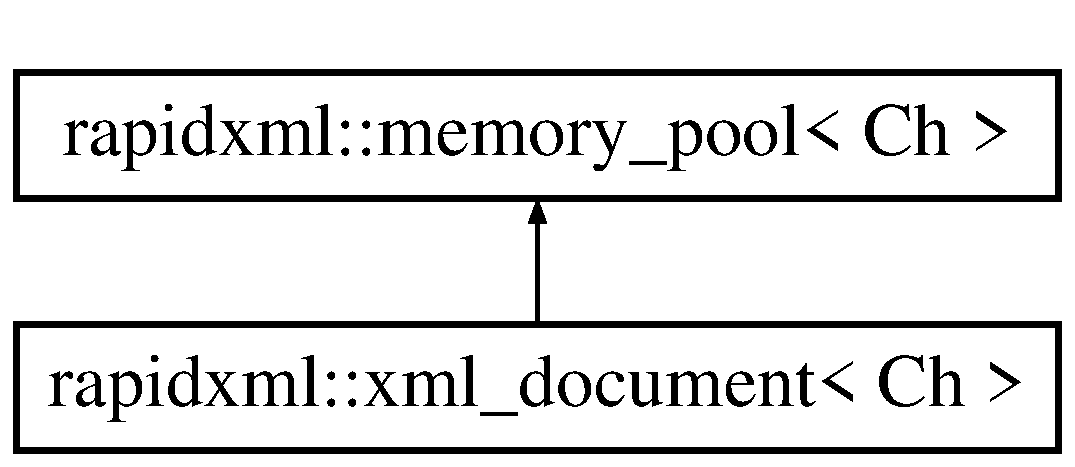
\includegraphics[height=2.000000cm]{classrapidxml_1_1memory__pool}
\end{center}
\end{figure}
\subsection*{Classes}
\begin{DoxyCompactItemize}
\item 
struct \hyperlink{structrapidxml_1_1memory__pool_1_1header}{header}
\end{DoxyCompactItemize}
\subsection*{Public Member Functions}
\begin{DoxyCompactItemize}
\item 
\hyperlink{classrapidxml_1_1memory__pool_a0b609da81dff28a19ebd704400788429}{memory\+\_\+pool} ()
\begin{DoxyCompactList}\small\item\em Constructs empty pool with default allocator functions. \end{DoxyCompactList}\item 
\hyperlink{classrapidxml_1_1memory__pool_a0a3e82126e59e4077f41e933130bb5a0}{$\sim$memory\+\_\+pool} ()
\item 
\hyperlink{classrapidxml_1_1xml__node}{xml\+\_\+node}$<$ Ch $>$ $\ast$ \hyperlink{classrapidxml_1_1memory__pool_a4118581c29ee9a2f6b55ebf7dac185f8}{allocate\+\_\+node} (\hyperlink{namespacerapidxml_abb456db38f7efb746c4330eed6072a7c}{node\+\_\+type} type, const Ch $\ast$name=0, const Ch $\ast$value=0, std\+::size\+\_\+t name\+\_\+size=0, std\+::size\+\_\+t value\+\_\+size=0)
\item 
\hyperlink{classrapidxml_1_1xml__attribute}{xml\+\_\+attribute}$<$ Ch $>$ $\ast$ \hyperlink{classrapidxml_1_1memory__pool_a3de2a66c983336e006ea3844e244ed30}{allocate\+\_\+attribute} (const Ch $\ast$name=0, const Ch $\ast$value=0, std\+::size\+\_\+t name\+\_\+size=0, std\+::size\+\_\+t value\+\_\+size=0)
\item 
Ch $\ast$ \hyperlink{classrapidxml_1_1memory__pool_a171941b39d55b868358da97462185f58}{allocate\+\_\+string} (const Ch $\ast$source=0, std\+::size\+\_\+t size=0)
\item 
\hyperlink{classrapidxml_1_1xml__node}{xml\+\_\+node}$<$ Ch $>$ $\ast$ \hyperlink{classrapidxml_1_1memory__pool_a0a10679fc17597d339a0dc107f8a94ac}{clone\+\_\+node} (const \hyperlink{classrapidxml_1_1xml__node}{xml\+\_\+node}$<$ Ch $>$ $\ast$source, \hyperlink{classrapidxml_1_1xml__node}{xml\+\_\+node}$<$ Ch $>$ $\ast$result=0)
\item 
void \hyperlink{classrapidxml_1_1memory__pool_aad377c835fdaed1cb2cc9df194cf84e4}{clear} ()
\item 
void \hyperlink{classrapidxml_1_1memory__pool_a84d3d8d2cdfc00501e1dcf26d889ae03}{set\+\_\+allocator} (alloc\+\_\+func $\ast$af, free\+\_\+func $\ast$ff)
\end{DoxyCompactItemize}
\subsection*{Private Member Functions}
\begin{DoxyCompactItemize}
\item 
void \hyperlink{classrapidxml_1_1memory__pool_a1076043ef092e327e59dd988c1ba82fb}{init} ()
\item 
char $\ast$ \hyperlink{classrapidxml_1_1memory__pool_a317396afc1812f08b64a1dd9cde4039b}{align} (char $\ast$ptr)
\item 
char $\ast$ \hyperlink{classrapidxml_1_1memory__pool_a1aed504a747303352e05f61c6ccbbebb}{allocate\+\_\+raw} (std\+::size\+\_\+t size)
\item 
void $\ast$ \hyperlink{classrapidxml_1_1memory__pool_a4e9cf53fa5f9da3a8f31b754bd94b4ec}{allocate\+\_\+aligned} (std\+::size\+\_\+t size)
\end{DoxyCompactItemize}
\subsection*{Private Attributes}
\begin{DoxyCompactItemize}
\item 
char $\ast$ \hyperlink{classrapidxml_1_1memory__pool_a775205c5faa60b63385c24368d26d4e1}{m\+\_\+begin}
\item 
char $\ast$ \hyperlink{classrapidxml_1_1memory__pool_a4a89ff677c72afc163d1855cefc28013}{m\+\_\+ptr}
\item 
char $\ast$ \hyperlink{classrapidxml_1_1memory__pool_a6c9a83514446842518c9ffb7a38b76eb}{m\+\_\+end}
\item 
char \hyperlink{classrapidxml_1_1memory__pool_aacc5ca734ebfbef7f42251764eb396f4}{m\+\_\+static\+\_\+memory} \mbox{[}\hyperlink{rapidxml_8hpp_a001304844ab478e3b213749fc8d72ca2}{R\+A\+P\+I\+D\+X\+M\+L\+\_\+\+S\+T\+A\+T\+I\+C\+\_\+\+P\+O\+O\+L\+\_\+\+S\+I\+Z\+E}\mbox{]}
\item 
alloc\+\_\+func $\ast$ \hyperlink{classrapidxml_1_1memory__pool_ae8964773675d24f77a808356be773c1d}{m\+\_\+alloc\+\_\+func}
\item 
free\+\_\+func $\ast$ \hyperlink{classrapidxml_1_1memory__pool_af8f41565f4de167eb2f40ca20695f24d}{m\+\_\+free\+\_\+func}
\end{DoxyCompactItemize}


\subsection{Detailed Description}
\subsubsection*{template$<$class Ch = char$>$class rapidxml\+::memory\+\_\+pool$<$ Ch $>$}

This class is used by the parser to create new nodes and attributes, without overheads of dynamic memory allocation. In most cases, you will not need to use this class directly. However, if you need to create nodes manually or modify names/values of nodes, you are encouraged to use \hyperlink{classrapidxml_1_1memory__pool}{memory\+\_\+pool} of relevant \hyperlink{classrapidxml_1_1xml__document}{xml\+\_\+document} to allocate the memory. Not only is this faster than allocating them by using {\ttfamily new} operator, but also their lifetime will be tied to the lifetime of document, possibly simplyfing memory management. ~\newline
~\newline
 Call \hyperlink{classrapidxml_1_1memory__pool_a4118581c29ee9a2f6b55ebf7dac185f8}{allocate\+\_\+node()} or \hyperlink{classrapidxml_1_1memory__pool_a3de2a66c983336e006ea3844e244ed30}{allocate\+\_\+attribute()} functions to obtain new nodes or attributes from the pool. You can also call \hyperlink{classrapidxml_1_1memory__pool_a171941b39d55b868358da97462185f58}{allocate\+\_\+string()} function to allocate strings. Such strings can then be used as names or values of nodes without worrying about their lifetime. Note that there is no {\ttfamily free()} function -- all allocations are freed at once when \hyperlink{classrapidxml_1_1memory__pool_aad377c835fdaed1cb2cc9df194cf84e4}{clear()} function is called, or when the pool is destroyed. ~\newline
~\newline
 It is also possible to create a standalone \hyperlink{classrapidxml_1_1memory__pool}{memory\+\_\+pool}, and use it to allocate nodes, whose lifetime will not be tied to any document. ~\newline
~\newline
 Pool maintains {\ttfamily R\+A\+P\+I\+D\+X\+M\+L\+\_\+\+S\+T\+A\+T\+I\+C\+\_\+\+P\+O\+O\+L\+\_\+\+S\+I\+Z\+E} bytes of statically allocated memory. Until static memory is exhausted, no dynamic memory allocations are done. When static memory is exhausted, pool allocates additional blocks of memory of size {\ttfamily R\+A\+P\+I\+D\+X\+M\+L\+\_\+\+D\+Y\+N\+A\+M\+I\+C\+\_\+\+P\+O\+O\+L\+\_\+\+S\+I\+Z\+E} each, by using global {\ttfamily new\mbox{[}\mbox{]}} and {\ttfamily delete\mbox{[}\mbox{]}} operators. This behaviour can be changed by setting custom allocation routines. Use \hyperlink{classrapidxml_1_1memory__pool_a84d3d8d2cdfc00501e1dcf26d889ae03}{set\+\_\+allocator()} function to set them. ~\newline
~\newline
 Allocations for nodes, attributes and strings are aligned at {\ttfamily R\+A\+P\+I\+D\+X\+M\+L\+\_\+\+A\+L\+I\+G\+N\+M\+E\+N\+T} bytes. This value defaults to the size of pointer on target architecture. ~\newline
~\newline
 To obtain absolutely top performance from the parser, it is important that all nodes are allocated from a single, contiguous block of memory. Otherwise, cache misses when jumping between two (or more) disjoint blocks of memory can slow down parsing quite considerably. If required, you can tweak {\ttfamily R\+A\+P\+I\+D\+X\+M\+L\+\_\+\+S\+T\+A\+T\+I\+C\+\_\+\+P\+O\+O\+L\+\_\+\+S\+I\+Z\+E}, {\ttfamily R\+A\+P\+I\+D\+X\+M\+L\+\_\+\+D\+Y\+N\+A\+M\+I\+C\+\_\+\+P\+O\+O\+L\+\_\+\+S\+I\+Z\+E} and {\ttfamily R\+A\+P\+I\+D\+X\+M\+L\+\_\+\+A\+L\+I\+G\+N\+M\+E\+N\+T} to obtain best wasted memory to performance compromise. To do it, define their values before \hyperlink{rapidxml_8hpp}{rapidxml.\+hpp} file is included. 
\begin{DoxyParams}{Parameters}
{\em Ch} & Character type of created nodes. \\
\hline
\end{DoxyParams}


\subsection{Constructor \& Destructor Documentation}
\hypertarget{classrapidxml_1_1memory__pool_a0b609da81dff28a19ebd704400788429}{}\index{rapidxml\+::memory\+\_\+pool@{rapidxml\+::memory\+\_\+pool}!memory\+\_\+pool@{memory\+\_\+pool}}
\index{memory\+\_\+pool@{memory\+\_\+pool}!rapidxml\+::memory\+\_\+pool@{rapidxml\+::memory\+\_\+pool}}
\subsubsection[{memory\+\_\+pool}]{\setlength{\rightskip}{0pt plus 5cm}template$<$class Ch  = char$>$ {\bf rapidxml\+::memory\+\_\+pool}$<$ Ch $>$\+::{\bf memory\+\_\+pool} (
\begin{DoxyParamCaption}
{}
\end{DoxyParamCaption}
)\hspace{0.3cm}{\ttfamily [inline]}}\label{classrapidxml_1_1memory__pool_a0b609da81dff28a19ebd704400788429}


Constructs empty pool with default allocator functions. 

\hypertarget{classrapidxml_1_1memory__pool_a0a3e82126e59e4077f41e933130bb5a0}{}\index{rapidxml\+::memory\+\_\+pool@{rapidxml\+::memory\+\_\+pool}!````~memory\+\_\+pool@{$\sim$memory\+\_\+pool}}
\index{````~memory\+\_\+pool@{$\sim$memory\+\_\+pool}!rapidxml\+::memory\+\_\+pool@{rapidxml\+::memory\+\_\+pool}}
\subsubsection[{$\sim$memory\+\_\+pool}]{\setlength{\rightskip}{0pt plus 5cm}template$<$class Ch  = char$>$ {\bf rapidxml\+::memory\+\_\+pool}$<$ Ch $>$\+::$\sim${\bf memory\+\_\+pool} (
\begin{DoxyParamCaption}
{}
\end{DoxyParamCaption}
)\hspace{0.3cm}{\ttfamily [inline]}}\label{classrapidxml_1_1memory__pool_a0a3e82126e59e4077f41e933130bb5a0}
Destroys pool and frees all the memory. This causes memory occupied by nodes allocated by the pool to be freed. Nodes allocated from the pool are no longer valid. 

\subsection{Member Function Documentation}
\hypertarget{classrapidxml_1_1memory__pool_a317396afc1812f08b64a1dd9cde4039b}{}\index{rapidxml\+::memory\+\_\+pool@{rapidxml\+::memory\+\_\+pool}!align@{align}}
\index{align@{align}!rapidxml\+::memory\+\_\+pool@{rapidxml\+::memory\+\_\+pool}}
\subsubsection[{align}]{\setlength{\rightskip}{0pt plus 5cm}template$<$class Ch  = char$>$ char$\ast$ {\bf rapidxml\+::memory\+\_\+pool}$<$ Ch $>$\+::align (
\begin{DoxyParamCaption}
\item[{char $\ast$}]{ptr}
\end{DoxyParamCaption}
)\hspace{0.3cm}{\ttfamily [inline]}, {\ttfamily [private]}}\label{classrapidxml_1_1memory__pool_a317396afc1812f08b64a1dd9cde4039b}
\hypertarget{classrapidxml_1_1memory__pool_a4e9cf53fa5f9da3a8f31b754bd94b4ec}{}\index{rapidxml\+::memory\+\_\+pool@{rapidxml\+::memory\+\_\+pool}!allocate\+\_\+aligned@{allocate\+\_\+aligned}}
\index{allocate\+\_\+aligned@{allocate\+\_\+aligned}!rapidxml\+::memory\+\_\+pool@{rapidxml\+::memory\+\_\+pool}}
\subsubsection[{allocate\+\_\+aligned}]{\setlength{\rightskip}{0pt plus 5cm}template$<$class Ch  = char$>$ void$\ast$ {\bf rapidxml\+::memory\+\_\+pool}$<$ Ch $>$\+::allocate\+\_\+aligned (
\begin{DoxyParamCaption}
\item[{std\+::size\+\_\+t}]{size}
\end{DoxyParamCaption}
)\hspace{0.3cm}{\ttfamily [inline]}, {\ttfamily [private]}}\label{classrapidxml_1_1memory__pool_a4e9cf53fa5f9da3a8f31b754bd94b4ec}
\hypertarget{classrapidxml_1_1memory__pool_a3de2a66c983336e006ea3844e244ed30}{}\index{rapidxml\+::memory\+\_\+pool@{rapidxml\+::memory\+\_\+pool}!allocate\+\_\+attribute@{allocate\+\_\+attribute}}
\index{allocate\+\_\+attribute@{allocate\+\_\+attribute}!rapidxml\+::memory\+\_\+pool@{rapidxml\+::memory\+\_\+pool}}
\subsubsection[{allocate\+\_\+attribute}]{\setlength{\rightskip}{0pt plus 5cm}template$<$class Ch  = char$>$ {\bf xml\+\_\+attribute}$<$Ch$>$$\ast$ {\bf rapidxml\+::memory\+\_\+pool}$<$ Ch $>$\+::allocate\+\_\+attribute (
\begin{DoxyParamCaption}
\item[{const Ch $\ast$}]{name = {\ttfamily 0}, }
\item[{const Ch $\ast$}]{value = {\ttfamily 0}, }
\item[{std\+::size\+\_\+t}]{name\+\_\+size = {\ttfamily 0}, }
\item[{std\+::size\+\_\+t}]{value\+\_\+size = {\ttfamily 0}}
\end{DoxyParamCaption}
)\hspace{0.3cm}{\ttfamily [inline]}}\label{classrapidxml_1_1memory__pool_a3de2a66c983336e006ea3844e244ed30}
Allocates a new attribute from the pool, and optionally assigns name and value to it. If the allocation request cannot be accomodated, this function will throw {\ttfamily std\+::bad\+\_\+alloc}. If exceptions are disabled by defining R\+A\+P\+I\+D\+X\+M\+L\+\_\+\+N\+O\+\_\+\+E\+X\+C\+E\+P\+T\+I\+O\+N\+S, this function will call rapidxml\+::parse\+\_\+error\+\_\+handler() function. 
\begin{DoxyParams}{Parameters}
{\em name} & Name to assign to the attribute, or 0 to assign no name. \\
\hline
{\em value} & Value to assign to the attribute, or 0 to assign no value. \\
\hline
{\em name\+\_\+size} & Size of name to assign, or 0 to automatically calculate size from name string. \\
\hline
{\em value\+\_\+size} & Size of value to assign, or 0 to automatically calculate size from value string. \\
\hline
\end{DoxyParams}
\begin{DoxyReturn}{Returns}
Pointer to allocated attribute. This pointer will never be N\+U\+L\+L. 
\end{DoxyReturn}
\hypertarget{classrapidxml_1_1memory__pool_a4118581c29ee9a2f6b55ebf7dac185f8}{}\index{rapidxml\+::memory\+\_\+pool@{rapidxml\+::memory\+\_\+pool}!allocate\+\_\+node@{allocate\+\_\+node}}
\index{allocate\+\_\+node@{allocate\+\_\+node}!rapidxml\+::memory\+\_\+pool@{rapidxml\+::memory\+\_\+pool}}
\subsubsection[{allocate\+\_\+node}]{\setlength{\rightskip}{0pt plus 5cm}template$<$class Ch  = char$>$ {\bf xml\+\_\+node}$<$Ch$>$$\ast$ {\bf rapidxml\+::memory\+\_\+pool}$<$ Ch $>$\+::allocate\+\_\+node (
\begin{DoxyParamCaption}
\item[{{\bf node\+\_\+type}}]{type, }
\item[{const Ch $\ast$}]{name = {\ttfamily 0}, }
\item[{const Ch $\ast$}]{value = {\ttfamily 0}, }
\item[{std\+::size\+\_\+t}]{name\+\_\+size = {\ttfamily 0}, }
\item[{std\+::size\+\_\+t}]{value\+\_\+size = {\ttfamily 0}}
\end{DoxyParamCaption}
)\hspace{0.3cm}{\ttfamily [inline]}}\label{classrapidxml_1_1memory__pool_a4118581c29ee9a2f6b55ebf7dac185f8}
Allocates a new node from the pool, and optionally assigns name and value to it. If the allocation request cannot be accomodated, this function will throw {\ttfamily std\+::bad\+\_\+alloc}. If exceptions are disabled by defining R\+A\+P\+I\+D\+X\+M\+L\+\_\+\+N\+O\+\_\+\+E\+X\+C\+E\+P\+T\+I\+O\+N\+S, this function will call rapidxml\+::parse\+\_\+error\+\_\+handler() function. 
\begin{DoxyParams}{Parameters}
{\em type} & Type of node to create. \\
\hline
{\em name} & Name to assign to the node, or 0 to assign no name. \\
\hline
{\em value} & Value to assign to the node, or 0 to assign no value. \\
\hline
{\em name\+\_\+size} & Size of name to assign, or 0 to automatically calculate size from name string. \\
\hline
{\em value\+\_\+size} & Size of value to assign, or 0 to automatically calculate size from value string. \\
\hline
\end{DoxyParams}
\begin{DoxyReturn}{Returns}
Pointer to allocated node. This pointer will never be N\+U\+L\+L. 
\end{DoxyReturn}
\hypertarget{classrapidxml_1_1memory__pool_a1aed504a747303352e05f61c6ccbbebb}{}\index{rapidxml\+::memory\+\_\+pool@{rapidxml\+::memory\+\_\+pool}!allocate\+\_\+raw@{allocate\+\_\+raw}}
\index{allocate\+\_\+raw@{allocate\+\_\+raw}!rapidxml\+::memory\+\_\+pool@{rapidxml\+::memory\+\_\+pool}}
\subsubsection[{allocate\+\_\+raw}]{\setlength{\rightskip}{0pt plus 5cm}template$<$class Ch  = char$>$ char$\ast$ {\bf rapidxml\+::memory\+\_\+pool}$<$ Ch $>$\+::allocate\+\_\+raw (
\begin{DoxyParamCaption}
\item[{std\+::size\+\_\+t}]{size}
\end{DoxyParamCaption}
)\hspace{0.3cm}{\ttfamily [inline]}, {\ttfamily [private]}}\label{classrapidxml_1_1memory__pool_a1aed504a747303352e05f61c6ccbbebb}
\hypertarget{classrapidxml_1_1memory__pool_a171941b39d55b868358da97462185f58}{}\index{rapidxml\+::memory\+\_\+pool@{rapidxml\+::memory\+\_\+pool}!allocate\+\_\+string@{allocate\+\_\+string}}
\index{allocate\+\_\+string@{allocate\+\_\+string}!rapidxml\+::memory\+\_\+pool@{rapidxml\+::memory\+\_\+pool}}
\subsubsection[{allocate\+\_\+string}]{\setlength{\rightskip}{0pt plus 5cm}template$<$class Ch  = char$>$ Ch$\ast$ {\bf rapidxml\+::memory\+\_\+pool}$<$ Ch $>$\+::allocate\+\_\+string (
\begin{DoxyParamCaption}
\item[{const Ch $\ast$}]{source = {\ttfamily 0}, }
\item[{std\+::size\+\_\+t}]{size = {\ttfamily 0}}
\end{DoxyParamCaption}
)\hspace{0.3cm}{\ttfamily [inline]}}\label{classrapidxml_1_1memory__pool_a171941b39d55b868358da97462185f58}
Allocates a char array of given size from the pool, and optionally copies a given string to it. If the allocation request cannot be accomodated, this function will throw {\ttfamily std\+::bad\+\_\+alloc}. If exceptions are disabled by defining R\+A\+P\+I\+D\+X\+M\+L\+\_\+\+N\+O\+\_\+\+E\+X\+C\+E\+P\+T\+I\+O\+N\+S, this function will call rapidxml\+::parse\+\_\+error\+\_\+handler() function. 
\begin{DoxyParams}{Parameters}
{\em source} & String to initialize the allocated memory with, or 0 to not initialize it. \\
\hline
{\em size} & Number of characters to allocate, or zero to calculate it automatically from source string length; if size is 0, source string must be specified and null terminated. \\
\hline
\end{DoxyParams}
\begin{DoxyReturn}{Returns}
Pointer to allocated char array. This pointer will never be N\+U\+L\+L. 
\end{DoxyReturn}
\hypertarget{classrapidxml_1_1memory__pool_aad377c835fdaed1cb2cc9df194cf84e4}{}\index{rapidxml\+::memory\+\_\+pool@{rapidxml\+::memory\+\_\+pool}!clear@{clear}}
\index{clear@{clear}!rapidxml\+::memory\+\_\+pool@{rapidxml\+::memory\+\_\+pool}}
\subsubsection[{clear}]{\setlength{\rightskip}{0pt plus 5cm}template$<$class Ch  = char$>$ void {\bf rapidxml\+::memory\+\_\+pool}$<$ Ch $>$\+::clear (
\begin{DoxyParamCaption}
{}
\end{DoxyParamCaption}
)\hspace{0.3cm}{\ttfamily [inline]}}\label{classrapidxml_1_1memory__pool_aad377c835fdaed1cb2cc9df194cf84e4}
Clears the pool. This causes memory occupied by nodes allocated by the pool to be freed. Any nodes or strings allocated from the pool will no longer be valid. \hypertarget{classrapidxml_1_1memory__pool_a0a10679fc17597d339a0dc107f8a94ac}{}\index{rapidxml\+::memory\+\_\+pool@{rapidxml\+::memory\+\_\+pool}!clone\+\_\+node@{clone\+\_\+node}}
\index{clone\+\_\+node@{clone\+\_\+node}!rapidxml\+::memory\+\_\+pool@{rapidxml\+::memory\+\_\+pool}}
\subsubsection[{clone\+\_\+node}]{\setlength{\rightskip}{0pt plus 5cm}template$<$class Ch  = char$>$ {\bf xml\+\_\+node}$<$Ch$>$$\ast$ {\bf rapidxml\+::memory\+\_\+pool}$<$ Ch $>$\+::clone\+\_\+node (
\begin{DoxyParamCaption}
\item[{const {\bf xml\+\_\+node}$<$ Ch $>$ $\ast$}]{source, }
\item[{{\bf xml\+\_\+node}$<$ Ch $>$ $\ast$}]{result = {\ttfamily 0}}
\end{DoxyParamCaption}
)\hspace{0.3cm}{\ttfamily [inline]}}\label{classrapidxml_1_1memory__pool_a0a10679fc17597d339a0dc107f8a94ac}
Clones an \hyperlink{classrapidxml_1_1xml__node}{xml\+\_\+node} and its hierarchy of child nodes and attributes. Nodes and attributes are allocated from this memory pool. Names and values are not cloned, they are shared between the clone and the source. Result node can be optionally specified as a second parameter, in which case its contents will be replaced with cloned source node. This is useful when you want to clone entire document. 
\begin{DoxyParams}{Parameters}
{\em source} & Node to clone. \\
\hline
{\em result} & Node to put results in, or 0 to automatically allocate result node \\
\hline
\end{DoxyParams}
\begin{DoxyReturn}{Returns}
Pointer to cloned node. This pointer will never be N\+U\+L\+L. 
\end{DoxyReturn}
\hypertarget{classrapidxml_1_1memory__pool_a1076043ef092e327e59dd988c1ba82fb}{}\index{rapidxml\+::memory\+\_\+pool@{rapidxml\+::memory\+\_\+pool}!init@{init}}
\index{init@{init}!rapidxml\+::memory\+\_\+pool@{rapidxml\+::memory\+\_\+pool}}
\subsubsection[{init}]{\setlength{\rightskip}{0pt plus 5cm}template$<$class Ch  = char$>$ void {\bf rapidxml\+::memory\+\_\+pool}$<$ Ch $>$\+::init (
\begin{DoxyParamCaption}
{}
\end{DoxyParamCaption}
)\hspace{0.3cm}{\ttfamily [inline]}, {\ttfamily [private]}}\label{classrapidxml_1_1memory__pool_a1076043ef092e327e59dd988c1ba82fb}
\hypertarget{classrapidxml_1_1memory__pool_a84d3d8d2cdfc00501e1dcf26d889ae03}{}\index{rapidxml\+::memory\+\_\+pool@{rapidxml\+::memory\+\_\+pool}!set\+\_\+allocator@{set\+\_\+allocator}}
\index{set\+\_\+allocator@{set\+\_\+allocator}!rapidxml\+::memory\+\_\+pool@{rapidxml\+::memory\+\_\+pool}}
\subsubsection[{set\+\_\+allocator}]{\setlength{\rightskip}{0pt plus 5cm}template$<$class Ch  = char$>$ void {\bf rapidxml\+::memory\+\_\+pool}$<$ Ch $>$\+::set\+\_\+allocator (
\begin{DoxyParamCaption}
\item[{alloc\+\_\+func $\ast$}]{af, }
\item[{free\+\_\+func $\ast$}]{ff}
\end{DoxyParamCaption}
)\hspace{0.3cm}{\ttfamily [inline]}}\label{classrapidxml_1_1memory__pool_a84d3d8d2cdfc00501e1dcf26d889ae03}
Sets or resets the user-\/defined memory allocation functions for the pool. This can only be called when no memory is allocated from the pool yet, otherwise results are undefined. Allocation function must not return invalid pointer on failure. It should either throw, stop the program, or use {\ttfamily longjmp()} function to pass control to other place of program. If it returns invalid pointer, results are undefined. ~\newline
~\newline
 User defined allocation functions must have the following forms\+: ~\newline
{\ttfamily  ~\newline
void $\ast$allocate(std\+::size\+\_\+t size); ~\newline
void free(void $\ast$pointer); }~\newline
 
\begin{DoxyParams}{Parameters}
{\em af} & Allocation function, or 0 to restore default function \\
\hline
{\em ff} & Free function, or 0 to restore default function \\
\hline
\end{DoxyParams}


\subsection{Member Data Documentation}
\hypertarget{classrapidxml_1_1memory__pool_ae8964773675d24f77a808356be773c1d}{}\index{rapidxml\+::memory\+\_\+pool@{rapidxml\+::memory\+\_\+pool}!m\+\_\+alloc\+\_\+func@{m\+\_\+alloc\+\_\+func}}
\index{m\+\_\+alloc\+\_\+func@{m\+\_\+alloc\+\_\+func}!rapidxml\+::memory\+\_\+pool@{rapidxml\+::memory\+\_\+pool}}
\subsubsection[{m\+\_\+alloc\+\_\+func}]{\setlength{\rightskip}{0pt plus 5cm}template$<$class Ch  = char$>$ alloc\+\_\+func$\ast$ {\bf rapidxml\+::memory\+\_\+pool}$<$ Ch $>$\+::m\+\_\+alloc\+\_\+func\hspace{0.3cm}{\ttfamily [private]}}\label{classrapidxml_1_1memory__pool_ae8964773675d24f77a808356be773c1d}
\hypertarget{classrapidxml_1_1memory__pool_a775205c5faa60b63385c24368d26d4e1}{}\index{rapidxml\+::memory\+\_\+pool@{rapidxml\+::memory\+\_\+pool}!m\+\_\+begin@{m\+\_\+begin}}
\index{m\+\_\+begin@{m\+\_\+begin}!rapidxml\+::memory\+\_\+pool@{rapidxml\+::memory\+\_\+pool}}
\subsubsection[{m\+\_\+begin}]{\setlength{\rightskip}{0pt plus 5cm}template$<$class Ch  = char$>$ char$\ast$ {\bf rapidxml\+::memory\+\_\+pool}$<$ Ch $>$\+::m\+\_\+begin\hspace{0.3cm}{\ttfamily [private]}}\label{classrapidxml_1_1memory__pool_a775205c5faa60b63385c24368d26d4e1}
\hypertarget{classrapidxml_1_1memory__pool_a6c9a83514446842518c9ffb7a38b76eb}{}\index{rapidxml\+::memory\+\_\+pool@{rapidxml\+::memory\+\_\+pool}!m\+\_\+end@{m\+\_\+end}}
\index{m\+\_\+end@{m\+\_\+end}!rapidxml\+::memory\+\_\+pool@{rapidxml\+::memory\+\_\+pool}}
\subsubsection[{m\+\_\+end}]{\setlength{\rightskip}{0pt plus 5cm}template$<$class Ch  = char$>$ char$\ast$ {\bf rapidxml\+::memory\+\_\+pool}$<$ Ch $>$\+::m\+\_\+end\hspace{0.3cm}{\ttfamily [private]}}\label{classrapidxml_1_1memory__pool_a6c9a83514446842518c9ffb7a38b76eb}
\hypertarget{classrapidxml_1_1memory__pool_af8f41565f4de167eb2f40ca20695f24d}{}\index{rapidxml\+::memory\+\_\+pool@{rapidxml\+::memory\+\_\+pool}!m\+\_\+free\+\_\+func@{m\+\_\+free\+\_\+func}}
\index{m\+\_\+free\+\_\+func@{m\+\_\+free\+\_\+func}!rapidxml\+::memory\+\_\+pool@{rapidxml\+::memory\+\_\+pool}}
\subsubsection[{m\+\_\+free\+\_\+func}]{\setlength{\rightskip}{0pt plus 5cm}template$<$class Ch  = char$>$ free\+\_\+func$\ast$ {\bf rapidxml\+::memory\+\_\+pool}$<$ Ch $>$\+::m\+\_\+free\+\_\+func\hspace{0.3cm}{\ttfamily [private]}}\label{classrapidxml_1_1memory__pool_af8f41565f4de167eb2f40ca20695f24d}
\hypertarget{classrapidxml_1_1memory__pool_a4a89ff677c72afc163d1855cefc28013}{}\index{rapidxml\+::memory\+\_\+pool@{rapidxml\+::memory\+\_\+pool}!m\+\_\+ptr@{m\+\_\+ptr}}
\index{m\+\_\+ptr@{m\+\_\+ptr}!rapidxml\+::memory\+\_\+pool@{rapidxml\+::memory\+\_\+pool}}
\subsubsection[{m\+\_\+ptr}]{\setlength{\rightskip}{0pt plus 5cm}template$<$class Ch  = char$>$ char$\ast$ {\bf rapidxml\+::memory\+\_\+pool}$<$ Ch $>$\+::m\+\_\+ptr\hspace{0.3cm}{\ttfamily [private]}}\label{classrapidxml_1_1memory__pool_a4a89ff677c72afc163d1855cefc28013}
\hypertarget{classrapidxml_1_1memory__pool_aacc5ca734ebfbef7f42251764eb396f4}{}\index{rapidxml\+::memory\+\_\+pool@{rapidxml\+::memory\+\_\+pool}!m\+\_\+static\+\_\+memory@{m\+\_\+static\+\_\+memory}}
\index{m\+\_\+static\+\_\+memory@{m\+\_\+static\+\_\+memory}!rapidxml\+::memory\+\_\+pool@{rapidxml\+::memory\+\_\+pool}}
\subsubsection[{m\+\_\+static\+\_\+memory}]{\setlength{\rightskip}{0pt plus 5cm}template$<$class Ch  = char$>$ char {\bf rapidxml\+::memory\+\_\+pool}$<$ Ch $>$\+::m\+\_\+static\+\_\+memory\mbox{[}{\bf R\+A\+P\+I\+D\+X\+M\+L\+\_\+\+S\+T\+A\+T\+I\+C\+\_\+\+P\+O\+O\+L\+\_\+\+S\+I\+Z\+E}\mbox{]}\hspace{0.3cm}{\ttfamily [private]}}\label{classrapidxml_1_1memory__pool_aacc5ca734ebfbef7f42251764eb396f4}


The documentation for this class was generated from the following file\+:\begin{DoxyCompactItemize}
\item 
\hyperlink{rapidxml_8hpp}{rapidxml.\+hpp}\end{DoxyCompactItemize}

\hypertarget{classrapidxml_1_1node__iterator}{}\section{rapidxml\+:\+:node\+\_\+iterator$<$ Ch $>$ Class Template Reference}
\label{classrapidxml_1_1node__iterator}\index{rapidxml\+::node\+\_\+iterator$<$ Ch $>$@{rapidxml\+::node\+\_\+iterator$<$ Ch $>$}}


Iterator of child nodes of \hyperlink{classrapidxml_1_1xml__node}{xml\+\_\+node}.  




{\ttfamily \#include $<$rapidxml\+\_\+iterators.\+hpp$>$}

\subsection*{Public Types}
\begin{DoxyCompactItemize}
\item 
typedef \hyperlink{classrapidxml_1_1xml__node}{xml\+\_\+node}$<$ Ch $>$ \hyperlink{classrapidxml_1_1node__iterator_ade6310119ed1f72c94830e006fac69b7}{value\+\_\+type}
\item 
typedef \hyperlink{classrapidxml_1_1xml__node}{xml\+\_\+node}$<$ Ch $>$ \& \hyperlink{classrapidxml_1_1node__iterator_ad7fabbcb7d3d9e4e220299c5475b9e9c}{reference}
\item 
typedef \hyperlink{classrapidxml_1_1xml__node}{xml\+\_\+node}$<$ Ch $>$ $\ast$ \hyperlink{classrapidxml_1_1node__iterator_a65dca8bca2b9c29f635b9ad0bdeeecb9}{pointer}
\item 
typedef std\+::ptrdiff\+\_\+t \hyperlink{classrapidxml_1_1node__iterator_a5bdc462b980a52c5fa2d99ac9f4f4bff}{difference\+\_\+type}
\item 
typedef std\+::bidirectional\+\_\+iterator\+\_\+tag \hyperlink{classrapidxml_1_1node__iterator_a8e82d75f768e17bf7349d010ee26c037}{iterator\+\_\+category}
\end{DoxyCompactItemize}
\subsection*{Public Member Functions}
\begin{DoxyCompactItemize}
\item 
\hyperlink{classrapidxml_1_1node__iterator_a4e1244b9e9e1d2b5129235806d1e31ad}{node\+\_\+iterator} ()
\item 
\hyperlink{classrapidxml_1_1node__iterator_a94c3da59b54e4bd003e226cc35b3c266}{node\+\_\+iterator} (\hyperlink{classrapidxml_1_1xml__node}{xml\+\_\+node}$<$ Ch $>$ $\ast$node)
\item 
\hyperlink{classrapidxml_1_1node__iterator_ad7fabbcb7d3d9e4e220299c5475b9e9c}{reference} \hyperlink{classrapidxml_1_1node__iterator_ab31fe5bc1fd01fee8a2b31c3e42d78ed}{operator$\ast$} () const 
\item 
\hyperlink{classrapidxml_1_1node__iterator_a65dca8bca2b9c29f635b9ad0bdeeecb9}{pointer} \hyperlink{classrapidxml_1_1node__iterator_a9b3e7d58c4a628524914932e0663ddfb}{operator-\/$>$} () const 
\item 
\hyperlink{classrapidxml_1_1node__iterator}{node\+\_\+iterator} \& \hyperlink{classrapidxml_1_1node__iterator_a8d6b184a76b2ec8a8b5e90bc013c80ed}{operator++} ()
\item 
\hyperlink{classrapidxml_1_1node__iterator}{node\+\_\+iterator} \hyperlink{classrapidxml_1_1node__iterator_ad01b4e43e348a330984833fd4924d0f2}{operator++} (int)
\item 
\hyperlink{classrapidxml_1_1node__iterator}{node\+\_\+iterator} \& \hyperlink{classrapidxml_1_1node__iterator_ace52107ecd1bcf02e49619e86206e3a3}{operator-\/-\/} ()
\item 
\hyperlink{classrapidxml_1_1node__iterator}{node\+\_\+iterator} \hyperlink{classrapidxml_1_1node__iterator_a4ca35716bb7865f199a137b063af6080}{operator-\/-\/} (int)
\item 
bool \hyperlink{classrapidxml_1_1node__iterator_a5cb8a3b0d65a1a2517995e986a4debfd}{operator==} (const \hyperlink{classrapidxml_1_1node__iterator}{node\+\_\+iterator}$<$ Ch $>$ \&rhs)
\item 
bool \hyperlink{classrapidxml_1_1node__iterator_a20f1e25347d7e3856694f18597f7c8e2}{operator!=} (const \hyperlink{classrapidxml_1_1node__iterator}{node\+\_\+iterator}$<$ Ch $>$ \&rhs)
\end{DoxyCompactItemize}
\subsection*{Private Attributes}
\begin{DoxyCompactItemize}
\item 
\hyperlink{classrapidxml_1_1xml__node}{xml\+\_\+node}$<$ Ch $>$ $\ast$ \hyperlink{classrapidxml_1_1node__iterator_adeb3cd87d8ea08aa56d14166146fa291}{m\+\_\+node}
\end{DoxyCompactItemize}


\subsection{Detailed Description}
\subsubsection*{template$<$class Ch$>$class rapidxml\+::node\+\_\+iterator$<$ Ch $>$}

Iterator of child nodes of \hyperlink{classrapidxml_1_1xml__node}{xml\+\_\+node}. 

\subsection{Member Typedef Documentation}
\hypertarget{classrapidxml_1_1node__iterator_a5bdc462b980a52c5fa2d99ac9f4f4bff}{}\index{rapidxml\+::node\+\_\+iterator@{rapidxml\+::node\+\_\+iterator}!difference\+\_\+type@{difference\+\_\+type}}
\index{difference\+\_\+type@{difference\+\_\+type}!rapidxml\+::node\+\_\+iterator@{rapidxml\+::node\+\_\+iterator}}
\subsubsection[{difference\+\_\+type}]{\setlength{\rightskip}{0pt plus 5cm}template$<$class Ch$>$ typedef std\+::ptrdiff\+\_\+t {\bf rapidxml\+::node\+\_\+iterator}$<$ Ch $>$\+::{\bf difference\+\_\+type}}\label{classrapidxml_1_1node__iterator_a5bdc462b980a52c5fa2d99ac9f4f4bff}
\hypertarget{classrapidxml_1_1node__iterator_a8e82d75f768e17bf7349d010ee26c037}{}\index{rapidxml\+::node\+\_\+iterator@{rapidxml\+::node\+\_\+iterator}!iterator\+\_\+category@{iterator\+\_\+category}}
\index{iterator\+\_\+category@{iterator\+\_\+category}!rapidxml\+::node\+\_\+iterator@{rapidxml\+::node\+\_\+iterator}}
\subsubsection[{iterator\+\_\+category}]{\setlength{\rightskip}{0pt plus 5cm}template$<$class Ch$>$ typedef std\+::bidirectional\+\_\+iterator\+\_\+tag {\bf rapidxml\+::node\+\_\+iterator}$<$ Ch $>$\+::{\bf iterator\+\_\+category}}\label{classrapidxml_1_1node__iterator_a8e82d75f768e17bf7349d010ee26c037}
\hypertarget{classrapidxml_1_1node__iterator_a65dca8bca2b9c29f635b9ad0bdeeecb9}{}\index{rapidxml\+::node\+\_\+iterator@{rapidxml\+::node\+\_\+iterator}!pointer@{pointer}}
\index{pointer@{pointer}!rapidxml\+::node\+\_\+iterator@{rapidxml\+::node\+\_\+iterator}}
\subsubsection[{pointer}]{\setlength{\rightskip}{0pt plus 5cm}template$<$class Ch$>$ typedef {\bf xml\+\_\+node}$<$Ch$>$$\ast$ {\bf rapidxml\+::node\+\_\+iterator}$<$ Ch $>$\+::{\bf pointer}}\label{classrapidxml_1_1node__iterator_a65dca8bca2b9c29f635b9ad0bdeeecb9}
\hypertarget{classrapidxml_1_1node__iterator_ad7fabbcb7d3d9e4e220299c5475b9e9c}{}\index{rapidxml\+::node\+\_\+iterator@{rapidxml\+::node\+\_\+iterator}!reference@{reference}}
\index{reference@{reference}!rapidxml\+::node\+\_\+iterator@{rapidxml\+::node\+\_\+iterator}}
\subsubsection[{reference}]{\setlength{\rightskip}{0pt plus 5cm}template$<$class Ch$>$ typedef {\bf xml\+\_\+node}$<$Ch$>$\& {\bf rapidxml\+::node\+\_\+iterator}$<$ Ch $>$\+::{\bf reference}}\label{classrapidxml_1_1node__iterator_ad7fabbcb7d3d9e4e220299c5475b9e9c}
\hypertarget{classrapidxml_1_1node__iterator_ade6310119ed1f72c94830e006fac69b7}{}\index{rapidxml\+::node\+\_\+iterator@{rapidxml\+::node\+\_\+iterator}!value\+\_\+type@{value\+\_\+type}}
\index{value\+\_\+type@{value\+\_\+type}!rapidxml\+::node\+\_\+iterator@{rapidxml\+::node\+\_\+iterator}}
\subsubsection[{value\+\_\+type}]{\setlength{\rightskip}{0pt plus 5cm}template$<$class Ch$>$ typedef {\bf xml\+\_\+node}$<$Ch$>$ {\bf rapidxml\+::node\+\_\+iterator}$<$ Ch $>$\+::{\bf value\+\_\+type}}\label{classrapidxml_1_1node__iterator_ade6310119ed1f72c94830e006fac69b7}


\subsection{Constructor \& Destructor Documentation}
\hypertarget{classrapidxml_1_1node__iterator_a4e1244b9e9e1d2b5129235806d1e31ad}{}\index{rapidxml\+::node\+\_\+iterator@{rapidxml\+::node\+\_\+iterator}!node\+\_\+iterator@{node\+\_\+iterator}}
\index{node\+\_\+iterator@{node\+\_\+iterator}!rapidxml\+::node\+\_\+iterator@{rapidxml\+::node\+\_\+iterator}}
\subsubsection[{node\+\_\+iterator}]{\setlength{\rightskip}{0pt plus 5cm}template$<$class Ch$>$ {\bf rapidxml\+::node\+\_\+iterator}$<$ Ch $>$\+::{\bf node\+\_\+iterator} (
\begin{DoxyParamCaption}
{}
\end{DoxyParamCaption}
)\hspace{0.3cm}{\ttfamily [inline]}}\label{classrapidxml_1_1node__iterator_a4e1244b9e9e1d2b5129235806d1e31ad}
\hypertarget{classrapidxml_1_1node__iterator_a94c3da59b54e4bd003e226cc35b3c266}{}\index{rapidxml\+::node\+\_\+iterator@{rapidxml\+::node\+\_\+iterator}!node\+\_\+iterator@{node\+\_\+iterator}}
\index{node\+\_\+iterator@{node\+\_\+iterator}!rapidxml\+::node\+\_\+iterator@{rapidxml\+::node\+\_\+iterator}}
\subsubsection[{node\+\_\+iterator}]{\setlength{\rightskip}{0pt plus 5cm}template$<$class Ch$>$ {\bf rapidxml\+::node\+\_\+iterator}$<$ Ch $>$\+::{\bf node\+\_\+iterator} (
\begin{DoxyParamCaption}
\item[{{\bf xml\+\_\+node}$<$ Ch $>$ $\ast$}]{node}
\end{DoxyParamCaption}
)\hspace{0.3cm}{\ttfamily [inline]}}\label{classrapidxml_1_1node__iterator_a94c3da59b54e4bd003e226cc35b3c266}


\subsection{Member Function Documentation}
\hypertarget{classrapidxml_1_1node__iterator_a20f1e25347d7e3856694f18597f7c8e2}{}\index{rapidxml\+::node\+\_\+iterator@{rapidxml\+::node\+\_\+iterator}!operator"!=@{operator"!=}}
\index{operator"!=@{operator"!=}!rapidxml\+::node\+\_\+iterator@{rapidxml\+::node\+\_\+iterator}}
\subsubsection[{operator"!=}]{\setlength{\rightskip}{0pt plus 5cm}template$<$class Ch$>$ bool {\bf rapidxml\+::node\+\_\+iterator}$<$ Ch $>$\+::operator!= (
\begin{DoxyParamCaption}
\item[{const {\bf node\+\_\+iterator}$<$ Ch $>$ \&}]{rhs}
\end{DoxyParamCaption}
)\hspace{0.3cm}{\ttfamily [inline]}}\label{classrapidxml_1_1node__iterator_a20f1e25347d7e3856694f18597f7c8e2}
\hypertarget{classrapidxml_1_1node__iterator_ab31fe5bc1fd01fee8a2b31c3e42d78ed}{}\index{rapidxml\+::node\+\_\+iterator@{rapidxml\+::node\+\_\+iterator}!operator$\ast$@{operator$\ast$}}
\index{operator$\ast$@{operator$\ast$}!rapidxml\+::node\+\_\+iterator@{rapidxml\+::node\+\_\+iterator}}
\subsubsection[{operator$\ast$}]{\setlength{\rightskip}{0pt plus 5cm}template$<$class Ch$>$ {\bf reference} {\bf rapidxml\+::node\+\_\+iterator}$<$ Ch $>$\+::operator$\ast$ (
\begin{DoxyParamCaption}
{}
\end{DoxyParamCaption}
) const\hspace{0.3cm}{\ttfamily [inline]}}\label{classrapidxml_1_1node__iterator_ab31fe5bc1fd01fee8a2b31c3e42d78ed}
\hypertarget{classrapidxml_1_1node__iterator_a8d6b184a76b2ec8a8b5e90bc013c80ed}{}\index{rapidxml\+::node\+\_\+iterator@{rapidxml\+::node\+\_\+iterator}!operator++@{operator++}}
\index{operator++@{operator++}!rapidxml\+::node\+\_\+iterator@{rapidxml\+::node\+\_\+iterator}}
\subsubsection[{operator++}]{\setlength{\rightskip}{0pt plus 5cm}template$<$class Ch$>$ {\bf node\+\_\+iterator}\& {\bf rapidxml\+::node\+\_\+iterator}$<$ Ch $>$\+::operator++ (
\begin{DoxyParamCaption}
{}
\end{DoxyParamCaption}
)\hspace{0.3cm}{\ttfamily [inline]}}\label{classrapidxml_1_1node__iterator_a8d6b184a76b2ec8a8b5e90bc013c80ed}
\hypertarget{classrapidxml_1_1node__iterator_ad01b4e43e348a330984833fd4924d0f2}{}\index{rapidxml\+::node\+\_\+iterator@{rapidxml\+::node\+\_\+iterator}!operator++@{operator++}}
\index{operator++@{operator++}!rapidxml\+::node\+\_\+iterator@{rapidxml\+::node\+\_\+iterator}}
\subsubsection[{operator++}]{\setlength{\rightskip}{0pt plus 5cm}template$<$class Ch$>$ {\bf node\+\_\+iterator} {\bf rapidxml\+::node\+\_\+iterator}$<$ Ch $>$\+::operator++ (
\begin{DoxyParamCaption}
\item[{int}]{}
\end{DoxyParamCaption}
)\hspace{0.3cm}{\ttfamily [inline]}}\label{classrapidxml_1_1node__iterator_ad01b4e43e348a330984833fd4924d0f2}
\hypertarget{classrapidxml_1_1node__iterator_ace52107ecd1bcf02e49619e86206e3a3}{}\index{rapidxml\+::node\+\_\+iterator@{rapidxml\+::node\+\_\+iterator}!operator-\/-\/@{operator-\/-\/}}
\index{operator-\/-\/@{operator-\/-\/}!rapidxml\+::node\+\_\+iterator@{rapidxml\+::node\+\_\+iterator}}
\subsubsection[{operator-\/-\/}]{\setlength{\rightskip}{0pt plus 5cm}template$<$class Ch$>$ {\bf node\+\_\+iterator}\& {\bf rapidxml\+::node\+\_\+iterator}$<$ Ch $>$\+::operator-\/-\/ (
\begin{DoxyParamCaption}
{}
\end{DoxyParamCaption}
)\hspace{0.3cm}{\ttfamily [inline]}}\label{classrapidxml_1_1node__iterator_ace52107ecd1bcf02e49619e86206e3a3}
\hypertarget{classrapidxml_1_1node__iterator_a4ca35716bb7865f199a137b063af6080}{}\index{rapidxml\+::node\+\_\+iterator@{rapidxml\+::node\+\_\+iterator}!operator-\/-\/@{operator-\/-\/}}
\index{operator-\/-\/@{operator-\/-\/}!rapidxml\+::node\+\_\+iterator@{rapidxml\+::node\+\_\+iterator}}
\subsubsection[{operator-\/-\/}]{\setlength{\rightskip}{0pt plus 5cm}template$<$class Ch$>$ {\bf node\+\_\+iterator} {\bf rapidxml\+::node\+\_\+iterator}$<$ Ch $>$\+::operator-\/-\/ (
\begin{DoxyParamCaption}
\item[{int}]{}
\end{DoxyParamCaption}
)\hspace{0.3cm}{\ttfamily [inline]}}\label{classrapidxml_1_1node__iterator_a4ca35716bb7865f199a137b063af6080}
\hypertarget{classrapidxml_1_1node__iterator_a9b3e7d58c4a628524914932e0663ddfb}{}\index{rapidxml\+::node\+\_\+iterator@{rapidxml\+::node\+\_\+iterator}!operator-\/$>$@{operator-\/$>$}}
\index{operator-\/$>$@{operator-\/$>$}!rapidxml\+::node\+\_\+iterator@{rapidxml\+::node\+\_\+iterator}}
\subsubsection[{operator-\/$>$}]{\setlength{\rightskip}{0pt plus 5cm}template$<$class Ch$>$ {\bf pointer} {\bf rapidxml\+::node\+\_\+iterator}$<$ Ch $>$\+::operator-\/$>$ (
\begin{DoxyParamCaption}
{}
\end{DoxyParamCaption}
) const\hspace{0.3cm}{\ttfamily [inline]}}\label{classrapidxml_1_1node__iterator_a9b3e7d58c4a628524914932e0663ddfb}
\hypertarget{classrapidxml_1_1node__iterator_a5cb8a3b0d65a1a2517995e986a4debfd}{}\index{rapidxml\+::node\+\_\+iterator@{rapidxml\+::node\+\_\+iterator}!operator==@{operator==}}
\index{operator==@{operator==}!rapidxml\+::node\+\_\+iterator@{rapidxml\+::node\+\_\+iterator}}
\subsubsection[{operator==}]{\setlength{\rightskip}{0pt plus 5cm}template$<$class Ch$>$ bool {\bf rapidxml\+::node\+\_\+iterator}$<$ Ch $>$\+::operator== (
\begin{DoxyParamCaption}
\item[{const {\bf node\+\_\+iterator}$<$ Ch $>$ \&}]{rhs}
\end{DoxyParamCaption}
)\hspace{0.3cm}{\ttfamily [inline]}}\label{classrapidxml_1_1node__iterator_a5cb8a3b0d65a1a2517995e986a4debfd}


\subsection{Member Data Documentation}
\hypertarget{classrapidxml_1_1node__iterator_adeb3cd87d8ea08aa56d14166146fa291}{}\index{rapidxml\+::node\+\_\+iterator@{rapidxml\+::node\+\_\+iterator}!m\+\_\+node@{m\+\_\+node}}
\index{m\+\_\+node@{m\+\_\+node}!rapidxml\+::node\+\_\+iterator@{rapidxml\+::node\+\_\+iterator}}
\subsubsection[{m\+\_\+node}]{\setlength{\rightskip}{0pt plus 5cm}template$<$class Ch$>$ {\bf xml\+\_\+node}$<$Ch$>$$\ast$ {\bf rapidxml\+::node\+\_\+iterator}$<$ Ch $>$\+::m\+\_\+node\hspace{0.3cm}{\ttfamily [private]}}\label{classrapidxml_1_1node__iterator_adeb3cd87d8ea08aa56d14166146fa291}


The documentation for this class was generated from the following file\+:\begin{DoxyCompactItemize}
\item 
\hyperlink{rapidxml__iterators_8hpp}{rapidxml\+\_\+iterators.\+hpp}\end{DoxyCompactItemize}

\hypertarget{structrapidxml_1_1xml__document_1_1node__name__pred}{}\section{rapidxml\+:\+:xml\+\_\+document$<$ Ch $>$\+:\+:node\+\_\+name\+\_\+pred Struct Reference}
\label{structrapidxml_1_1xml__document_1_1node__name__pred}\index{rapidxml\+::xml\+\_\+document$<$ Ch $>$\+::node\+\_\+name\+\_\+pred@{rapidxml\+::xml\+\_\+document$<$ Ch $>$\+::node\+\_\+name\+\_\+pred}}
\subsection*{Static Public Member Functions}
\begin{DoxyCompactItemize}
\item 
static unsigned char \hyperlink{structrapidxml_1_1xml__document_1_1node__name__pred_a4eb7916489a3d057a340ce84e9135aec}{test} (Ch ch)
\end{DoxyCompactItemize}


\subsection{Member Function Documentation}
\hypertarget{structrapidxml_1_1xml__document_1_1node__name__pred_a4eb7916489a3d057a340ce84e9135aec}{}\index{rapidxml\+::xml\+\_\+document\+::node\+\_\+name\+\_\+pred@{rapidxml\+::xml\+\_\+document\+::node\+\_\+name\+\_\+pred}!test@{test}}
\index{test@{test}!rapidxml\+::xml\+\_\+document\+::node\+\_\+name\+\_\+pred@{rapidxml\+::xml\+\_\+document\+::node\+\_\+name\+\_\+pred}}
\subsubsection[{test}]{\setlength{\rightskip}{0pt plus 5cm}template$<$class Ch  = char$>$ static unsigned char {\bf rapidxml\+::xml\+\_\+document}$<$ Ch $>$\+::node\+\_\+name\+\_\+pred\+::test (
\begin{DoxyParamCaption}
\item[{Ch}]{ch}
\end{DoxyParamCaption}
)\hspace{0.3cm}{\ttfamily [inline]}, {\ttfamily [static]}}\label{structrapidxml_1_1xml__document_1_1node__name__pred_a4eb7916489a3d057a340ce84e9135aec}


The documentation for this struct was generated from the following file\+:\begin{DoxyCompactItemize}
\item 
\hyperlink{rapidxml_8hpp}{rapidxml.\+hpp}\end{DoxyCompactItemize}

\hypertarget{class_page_info}{}\section{Page\+Info Class Reference}
\label{class_page_info}\index{Page\+Info@{Page\+Info}}


{\ttfamily \#include $<$pageinfo.\+h$>$}

\subsection*{Public Member Functions}
\begin{DoxyCompactItemize}
\item 
\hyperlink{class_page_info_a3ab3b93ca3b3d09645d5e187863b84e6}{Page\+Info} ()
\item 
\hyperlink{class_page_info_a45259793eed3f830dadecfde0e970ec5}{$\sim$\+Page\+Info} ()
\item 
\hyperlink{class_page_info_aa98a49dd45fdea434a27e4892dbdf032}{Page\+Info} (string the\+Content, string the\+Contributor, string the\+Timestamp, string the\+Title)
\item 
string \hyperlink{class_page_info_a61bd04fcecb67f3fac9833cd4a0e432b}{get\+\_\+content} ()
\item 
string \hyperlink{class_page_info_a6569fb1fd2a7efa4a6d144aa87c27912}{get\+\_\+contributor} ()
\item 
string \hyperlink{class_page_info_ab2fa01ac638b965912b93fce36d4899a}{get\+\_\+timestamp} ()
\item 
string \hyperlink{class_page_info_a0985d632ae64c913fe976bedccaf5d31}{get\+\_\+title} ()
\item 
int \hyperlink{class_page_info_a40938f3d2f1c81079abcbe8051143d53}{get\+\_\+total\+Words} ()
\item 
void \hyperlink{class_page_info_afaf6005be3e5fa629619038a96fbd1af}{set\+\_\+content} (string the\+Content)
\item 
void \hyperlink{class_page_info_afb03f9cd31ec6e6f500393cd5c7e1037}{set\+\_\+contributor} (string the\+Info)
\item 
void \hyperlink{class_page_info_ad8f8aada94adc772c9739f5dcb3223a7}{set\+\_\+timestamp} (string the\+Timestamp)
\item 
void \hyperlink{class_page_info_a0808f61697bbeca2d717d9b55b233ae1}{set\+\_\+title} (string the\+Title)
\item 
void \hyperlink{class_page_info_a43de865e72ac2fc61f124e2acee9da4d}{incr\+\_\+total\+Words} (int incr)
\item 
void \hyperlink{class_page_info_adcd293f9d6bdc291f7f28663e7151c45}{set\+\_\+total\+Words} (int the\+Total)
\end{DoxyCompactItemize}
\subsection*{Private Attributes}
\begin{DoxyCompactItemize}
\item 
string \hyperlink{class_page_info_a41470b013a300fe2ba52c7caae33e7b3}{content}
\item 
string \hyperlink{class_page_info_ab82a31135a4d68130b132fcf0503b317}{contributor\+Name\+Or\+I\+P}
\item 
string \hyperlink{class_page_info_a10e7ce551d454c4bf3ca50c4cad5496b}{timestamp}
\item 
string \hyperlink{class_page_info_adc9cfe7cc103f083fab4f3575eb073e1}{title}
\item 
int \hyperlink{class_page_info_aca7e985b3d5879e5bbe030b63a523393}{total\+Words}
\end{DoxyCompactItemize}


\subsection{Constructor \& Destructor Documentation}
\hypertarget{class_page_info_a3ab3b93ca3b3d09645d5e187863b84e6}{}\index{Page\+Info@{Page\+Info}!Page\+Info@{Page\+Info}}
\index{Page\+Info@{Page\+Info}!Page\+Info@{Page\+Info}}
\subsubsection[{Page\+Info}]{\setlength{\rightskip}{0pt plus 5cm}Page\+Info\+::\+Page\+Info (
\begin{DoxyParamCaption}
{}
\end{DoxyParamCaption}
)}\label{class_page_info_a3ab3b93ca3b3d09645d5e187863b84e6}
\hypertarget{class_page_info_a45259793eed3f830dadecfde0e970ec5}{}\index{Page\+Info@{Page\+Info}!````~Page\+Info@{$\sim$\+Page\+Info}}
\index{````~Page\+Info@{$\sim$\+Page\+Info}!Page\+Info@{Page\+Info}}
\subsubsection[{$\sim$\+Page\+Info}]{\setlength{\rightskip}{0pt plus 5cm}Page\+Info\+::$\sim$\+Page\+Info (
\begin{DoxyParamCaption}
{}
\end{DoxyParamCaption}
)}\label{class_page_info_a45259793eed3f830dadecfde0e970ec5}
\hypertarget{class_page_info_aa98a49dd45fdea434a27e4892dbdf032}{}\index{Page\+Info@{Page\+Info}!Page\+Info@{Page\+Info}}
\index{Page\+Info@{Page\+Info}!Page\+Info@{Page\+Info}}
\subsubsection[{Page\+Info}]{\setlength{\rightskip}{0pt plus 5cm}Page\+Info\+::\+Page\+Info (
\begin{DoxyParamCaption}
\item[{string}]{the\+Content, }
\item[{string}]{the\+Contributor, }
\item[{string}]{the\+Timestamp, }
\item[{string}]{the\+Title}
\end{DoxyParamCaption}
)}\label{class_page_info_aa98a49dd45fdea434a27e4892dbdf032}


\subsection{Member Function Documentation}
\hypertarget{class_page_info_a61bd04fcecb67f3fac9833cd4a0e432b}{}\index{Page\+Info@{Page\+Info}!get\+\_\+content@{get\+\_\+content}}
\index{get\+\_\+content@{get\+\_\+content}!Page\+Info@{Page\+Info}}
\subsubsection[{get\+\_\+content}]{\setlength{\rightskip}{0pt plus 5cm}string Page\+Info\+::get\+\_\+content (
\begin{DoxyParamCaption}
{}
\end{DoxyParamCaption}
)}\label{class_page_info_a61bd04fcecb67f3fac9833cd4a0e432b}
\hypertarget{class_page_info_a6569fb1fd2a7efa4a6d144aa87c27912}{}\index{Page\+Info@{Page\+Info}!get\+\_\+contributor@{get\+\_\+contributor}}
\index{get\+\_\+contributor@{get\+\_\+contributor}!Page\+Info@{Page\+Info}}
\subsubsection[{get\+\_\+contributor}]{\setlength{\rightskip}{0pt plus 5cm}string Page\+Info\+::get\+\_\+contributor (
\begin{DoxyParamCaption}
{}
\end{DoxyParamCaption}
)}\label{class_page_info_a6569fb1fd2a7efa4a6d144aa87c27912}
\hypertarget{class_page_info_ab2fa01ac638b965912b93fce36d4899a}{}\index{Page\+Info@{Page\+Info}!get\+\_\+timestamp@{get\+\_\+timestamp}}
\index{get\+\_\+timestamp@{get\+\_\+timestamp}!Page\+Info@{Page\+Info}}
\subsubsection[{get\+\_\+timestamp}]{\setlength{\rightskip}{0pt plus 5cm}string Page\+Info\+::get\+\_\+timestamp (
\begin{DoxyParamCaption}
{}
\end{DoxyParamCaption}
)}\label{class_page_info_ab2fa01ac638b965912b93fce36d4899a}
\hypertarget{class_page_info_a0985d632ae64c913fe976bedccaf5d31}{}\index{Page\+Info@{Page\+Info}!get\+\_\+title@{get\+\_\+title}}
\index{get\+\_\+title@{get\+\_\+title}!Page\+Info@{Page\+Info}}
\subsubsection[{get\+\_\+title}]{\setlength{\rightskip}{0pt plus 5cm}string Page\+Info\+::get\+\_\+title (
\begin{DoxyParamCaption}
{}
\end{DoxyParamCaption}
)}\label{class_page_info_a0985d632ae64c913fe976bedccaf5d31}
\hypertarget{class_page_info_a40938f3d2f1c81079abcbe8051143d53}{}\index{Page\+Info@{Page\+Info}!get\+\_\+total\+Words@{get\+\_\+total\+Words}}
\index{get\+\_\+total\+Words@{get\+\_\+total\+Words}!Page\+Info@{Page\+Info}}
\subsubsection[{get\+\_\+total\+Words}]{\setlength{\rightskip}{0pt plus 5cm}int Page\+Info\+::get\+\_\+total\+Words (
\begin{DoxyParamCaption}
{}
\end{DoxyParamCaption}
)}\label{class_page_info_a40938f3d2f1c81079abcbe8051143d53}
\hypertarget{class_page_info_a43de865e72ac2fc61f124e2acee9da4d}{}\index{Page\+Info@{Page\+Info}!incr\+\_\+total\+Words@{incr\+\_\+total\+Words}}
\index{incr\+\_\+total\+Words@{incr\+\_\+total\+Words}!Page\+Info@{Page\+Info}}
\subsubsection[{incr\+\_\+total\+Words}]{\setlength{\rightskip}{0pt plus 5cm}void Page\+Info\+::incr\+\_\+total\+Words (
\begin{DoxyParamCaption}
\item[{int}]{incr}
\end{DoxyParamCaption}
)}\label{class_page_info_a43de865e72ac2fc61f124e2acee9da4d}
\hypertarget{class_page_info_afaf6005be3e5fa629619038a96fbd1af}{}\index{Page\+Info@{Page\+Info}!set\+\_\+content@{set\+\_\+content}}
\index{set\+\_\+content@{set\+\_\+content}!Page\+Info@{Page\+Info}}
\subsubsection[{set\+\_\+content}]{\setlength{\rightskip}{0pt plus 5cm}void Page\+Info\+::set\+\_\+content (
\begin{DoxyParamCaption}
\item[{string}]{the\+Content}
\end{DoxyParamCaption}
)}\label{class_page_info_afaf6005be3e5fa629619038a96fbd1af}
\hypertarget{class_page_info_afb03f9cd31ec6e6f500393cd5c7e1037}{}\index{Page\+Info@{Page\+Info}!set\+\_\+contributor@{set\+\_\+contributor}}
\index{set\+\_\+contributor@{set\+\_\+contributor}!Page\+Info@{Page\+Info}}
\subsubsection[{set\+\_\+contributor}]{\setlength{\rightskip}{0pt plus 5cm}void Page\+Info\+::set\+\_\+contributor (
\begin{DoxyParamCaption}
\item[{string}]{the\+Info}
\end{DoxyParamCaption}
)}\label{class_page_info_afb03f9cd31ec6e6f500393cd5c7e1037}
\hypertarget{class_page_info_ad8f8aada94adc772c9739f5dcb3223a7}{}\index{Page\+Info@{Page\+Info}!set\+\_\+timestamp@{set\+\_\+timestamp}}
\index{set\+\_\+timestamp@{set\+\_\+timestamp}!Page\+Info@{Page\+Info}}
\subsubsection[{set\+\_\+timestamp}]{\setlength{\rightskip}{0pt plus 5cm}void Page\+Info\+::set\+\_\+timestamp (
\begin{DoxyParamCaption}
\item[{string}]{the\+Timestamp}
\end{DoxyParamCaption}
)}\label{class_page_info_ad8f8aada94adc772c9739f5dcb3223a7}
\hypertarget{class_page_info_a0808f61697bbeca2d717d9b55b233ae1}{}\index{Page\+Info@{Page\+Info}!set\+\_\+title@{set\+\_\+title}}
\index{set\+\_\+title@{set\+\_\+title}!Page\+Info@{Page\+Info}}
\subsubsection[{set\+\_\+title}]{\setlength{\rightskip}{0pt plus 5cm}void Page\+Info\+::set\+\_\+title (
\begin{DoxyParamCaption}
\item[{string}]{the\+Title}
\end{DoxyParamCaption}
)}\label{class_page_info_a0808f61697bbeca2d717d9b55b233ae1}
\hypertarget{class_page_info_adcd293f9d6bdc291f7f28663e7151c45}{}\index{Page\+Info@{Page\+Info}!set\+\_\+total\+Words@{set\+\_\+total\+Words}}
\index{set\+\_\+total\+Words@{set\+\_\+total\+Words}!Page\+Info@{Page\+Info}}
\subsubsection[{set\+\_\+total\+Words}]{\setlength{\rightskip}{0pt plus 5cm}void Page\+Info\+::set\+\_\+total\+Words (
\begin{DoxyParamCaption}
\item[{int}]{the\+Total}
\end{DoxyParamCaption}
)}\label{class_page_info_adcd293f9d6bdc291f7f28663e7151c45}


\subsection{Member Data Documentation}
\hypertarget{class_page_info_a41470b013a300fe2ba52c7caae33e7b3}{}\index{Page\+Info@{Page\+Info}!content@{content}}
\index{content@{content}!Page\+Info@{Page\+Info}}
\subsubsection[{content}]{\setlength{\rightskip}{0pt plus 5cm}string Page\+Info\+::content\hspace{0.3cm}{\ttfamily [private]}}\label{class_page_info_a41470b013a300fe2ba52c7caae33e7b3}
\hypertarget{class_page_info_ab82a31135a4d68130b132fcf0503b317}{}\index{Page\+Info@{Page\+Info}!contributor\+Name\+Or\+I\+P@{contributor\+Name\+Or\+I\+P}}
\index{contributor\+Name\+Or\+I\+P@{contributor\+Name\+Or\+I\+P}!Page\+Info@{Page\+Info}}
\subsubsection[{contributor\+Name\+Or\+I\+P}]{\setlength{\rightskip}{0pt plus 5cm}string Page\+Info\+::contributor\+Name\+Or\+I\+P\hspace{0.3cm}{\ttfamily [private]}}\label{class_page_info_ab82a31135a4d68130b132fcf0503b317}
\hypertarget{class_page_info_a10e7ce551d454c4bf3ca50c4cad5496b}{}\index{Page\+Info@{Page\+Info}!timestamp@{timestamp}}
\index{timestamp@{timestamp}!Page\+Info@{Page\+Info}}
\subsubsection[{timestamp}]{\setlength{\rightskip}{0pt plus 5cm}string Page\+Info\+::timestamp\hspace{0.3cm}{\ttfamily [private]}}\label{class_page_info_a10e7ce551d454c4bf3ca50c4cad5496b}
\hypertarget{class_page_info_adc9cfe7cc103f083fab4f3575eb073e1}{}\index{Page\+Info@{Page\+Info}!title@{title}}
\index{title@{title}!Page\+Info@{Page\+Info}}
\subsubsection[{title}]{\setlength{\rightskip}{0pt plus 5cm}string Page\+Info\+::title\hspace{0.3cm}{\ttfamily [private]}}\label{class_page_info_adc9cfe7cc103f083fab4f3575eb073e1}
\hypertarget{class_page_info_aca7e985b3d5879e5bbe030b63a523393}{}\index{Page\+Info@{Page\+Info}!total\+Words@{total\+Words}}
\index{total\+Words@{total\+Words}!Page\+Info@{Page\+Info}}
\subsubsection[{total\+Words}]{\setlength{\rightskip}{0pt plus 5cm}int Page\+Info\+::total\+Words\hspace{0.3cm}{\ttfamily [private]}}\label{class_page_info_aca7e985b3d5879e5bbe030b63a523393}


The documentation for this class was generated from the following files\+:\begin{DoxyCompactItemize}
\item 
\hyperlink{pageinfo_8h}{pageinfo.\+h}\item 
\hyperlink{pageinfo_8cpp}{pageinfo.\+cpp}\end{DoxyCompactItemize}

\hypertarget{classrapidxml_1_1parse__error}{}\section{rapidxml\+:\+:parse\+\_\+error Class Reference}
\label{classrapidxml_1_1parse__error}\index{rapidxml\+::parse\+\_\+error@{rapidxml\+::parse\+\_\+error}}


{\ttfamily \#include $<$rapidxml.\+hpp$>$}

Inheritance diagram for rapidxml\+:\+:parse\+\_\+error\+:\begin{figure}[H]
\begin{center}
\leavevmode
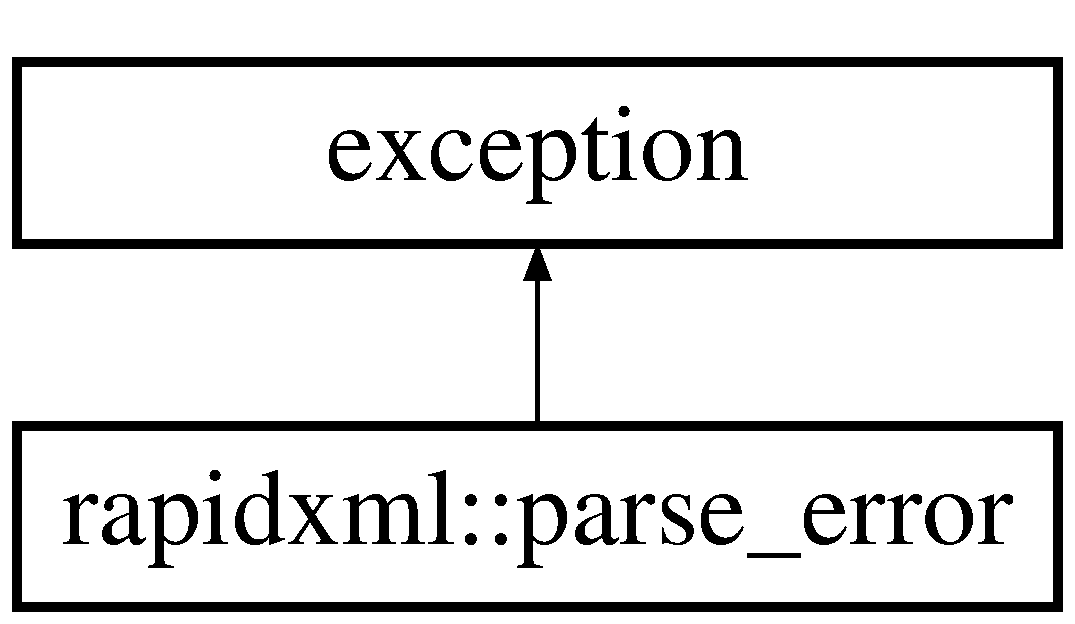
\includegraphics[height=2.000000cm]{classrapidxml_1_1parse__error}
\end{center}
\end{figure}
\subsection*{Public Member Functions}
\begin{DoxyCompactItemize}
\item 
\hyperlink{classrapidxml_1_1parse__error_aea12a301271c393fb627b368fb9f35c1}{parse\+\_\+error} (const char $\ast$\hyperlink{classrapidxml_1_1parse__error_a7665c88639e7466ee1de388a4f85e6fe}{what}, void $\ast$\hyperlink{classrapidxml_1_1parse__error_a3a0ab9e586c1d2b437c340f6622fbec6}{where})
\begin{DoxyCompactList}\small\item\em Constructs parse error. \end{DoxyCompactList}\item 
virtual const char $\ast$ \hyperlink{classrapidxml_1_1parse__error_a7665c88639e7466ee1de388a4f85e6fe}{what} () const   throw ()
\item 
{\footnotesize template$<$class Ch $>$ }\\Ch $\ast$ \hyperlink{classrapidxml_1_1parse__error_a3a0ab9e586c1d2b437c340f6622fbec6}{where} () const 
\end{DoxyCompactItemize}
\subsection*{Private Attributes}
\begin{DoxyCompactItemize}
\item 
const char $\ast$ \hyperlink{classrapidxml_1_1parse__error_a41bffadc72eec238cf4b7d14c10c16ca}{m\+\_\+what}
\item 
void $\ast$ \hyperlink{classrapidxml_1_1parse__error_aa5a164653ac347adddf47b264620d80f}{m\+\_\+where}
\end{DoxyCompactItemize}


\subsection{Detailed Description}
Parse error exception. This exception is thrown by the parser when an error occurs. Use \hyperlink{classrapidxml_1_1parse__error_a7665c88639e7466ee1de388a4f85e6fe}{what()} function to get human-\/readable error message. Use \hyperlink{classrapidxml_1_1parse__error_a3a0ab9e586c1d2b437c340f6622fbec6}{where()} function to get a pointer to position within source text where error was detected. ~\newline
~\newline
 If throwing exceptions by the parser is undesirable, it can be disabled by defining R\+A\+P\+I\+D\+X\+M\+L\+\_\+\+N\+O\+\_\+\+E\+X\+C\+E\+P\+T\+I\+O\+N\+S macro before \hyperlink{rapidxml_8hpp}{rapidxml.\+hpp} is included. This will cause the parser to call rapidxml\+::parse\+\_\+error\+\_\+handler() function instead of throwing an exception. This function must be defined by the user. ~\newline
~\newline
 This class derives from {\ttfamily std\+::exception} class. 

\subsection{Constructor \& Destructor Documentation}
\hypertarget{classrapidxml_1_1parse__error_aea12a301271c393fb627b368fb9f35c1}{}\index{rapidxml\+::parse\+\_\+error@{rapidxml\+::parse\+\_\+error}!parse\+\_\+error@{parse\+\_\+error}}
\index{parse\+\_\+error@{parse\+\_\+error}!rapidxml\+::parse\+\_\+error@{rapidxml\+::parse\+\_\+error}}
\subsubsection[{parse\+\_\+error}]{\setlength{\rightskip}{0pt plus 5cm}rapidxml\+::parse\+\_\+error\+::parse\+\_\+error (
\begin{DoxyParamCaption}
\item[{const char $\ast$}]{what, }
\item[{void $\ast$}]{where}
\end{DoxyParamCaption}
)\hspace{0.3cm}{\ttfamily [inline]}}\label{classrapidxml_1_1parse__error_aea12a301271c393fb627b368fb9f35c1}


Constructs parse error. 



\subsection{Member Function Documentation}
\hypertarget{classrapidxml_1_1parse__error_a7665c88639e7466ee1de388a4f85e6fe}{}\index{rapidxml\+::parse\+\_\+error@{rapidxml\+::parse\+\_\+error}!what@{what}}
\index{what@{what}!rapidxml\+::parse\+\_\+error@{rapidxml\+::parse\+\_\+error}}
\subsubsection[{what}]{\setlength{\rightskip}{0pt plus 5cm}virtual const char$\ast$ rapidxml\+::parse\+\_\+error\+::what (
\begin{DoxyParamCaption}
{}
\end{DoxyParamCaption}
) const throw  ) \hspace{0.3cm}{\ttfamily [inline]}, {\ttfamily [virtual]}}\label{classrapidxml_1_1parse__error_a7665c88639e7466ee1de388a4f85e6fe}
Gets human readable description of error. \begin{DoxyReturn}{Returns}
Pointer to null terminated description of the error. 
\end{DoxyReturn}
\hypertarget{classrapidxml_1_1parse__error_a3a0ab9e586c1d2b437c340f6622fbec6}{}\index{rapidxml\+::parse\+\_\+error@{rapidxml\+::parse\+\_\+error}!where@{where}}
\index{where@{where}!rapidxml\+::parse\+\_\+error@{rapidxml\+::parse\+\_\+error}}
\subsubsection[{where}]{\setlength{\rightskip}{0pt plus 5cm}template$<$class Ch $>$ Ch$\ast$ rapidxml\+::parse\+\_\+error\+::where (
\begin{DoxyParamCaption}
{}
\end{DoxyParamCaption}
) const\hspace{0.3cm}{\ttfamily [inline]}}\label{classrapidxml_1_1parse__error_a3a0ab9e586c1d2b437c340f6622fbec6}
Gets pointer to character data where error happened. Ch should be the same as char type of \hyperlink{classrapidxml_1_1xml__document}{xml\+\_\+document} that produced the error. \begin{DoxyReturn}{Returns}
Pointer to location within the parsed string where error occured. 
\end{DoxyReturn}


\subsection{Member Data Documentation}
\hypertarget{classrapidxml_1_1parse__error_a41bffadc72eec238cf4b7d14c10c16ca}{}\index{rapidxml\+::parse\+\_\+error@{rapidxml\+::parse\+\_\+error}!m\+\_\+what@{m\+\_\+what}}
\index{m\+\_\+what@{m\+\_\+what}!rapidxml\+::parse\+\_\+error@{rapidxml\+::parse\+\_\+error}}
\subsubsection[{m\+\_\+what}]{\setlength{\rightskip}{0pt plus 5cm}const char$\ast$ rapidxml\+::parse\+\_\+error\+::m\+\_\+what\hspace{0.3cm}{\ttfamily [private]}}\label{classrapidxml_1_1parse__error_a41bffadc72eec238cf4b7d14c10c16ca}
\hypertarget{classrapidxml_1_1parse__error_aa5a164653ac347adddf47b264620d80f}{}\index{rapidxml\+::parse\+\_\+error@{rapidxml\+::parse\+\_\+error}!m\+\_\+where@{m\+\_\+where}}
\index{m\+\_\+where@{m\+\_\+where}!rapidxml\+::parse\+\_\+error@{rapidxml\+::parse\+\_\+error}}
\subsubsection[{m\+\_\+where}]{\setlength{\rightskip}{0pt plus 5cm}void$\ast$ rapidxml\+::parse\+\_\+error\+::m\+\_\+where\hspace{0.3cm}{\ttfamily [private]}}\label{classrapidxml_1_1parse__error_aa5a164653ac347adddf47b264620d80f}


The documentation for this class was generated from the following file\+:\begin{DoxyCompactItemize}
\item 
\hyperlink{rapidxml_8hpp}{rapidxml.\+hpp}\end{DoxyCompactItemize}

\hypertarget{class_query_processor}{}\section{Query\+Processor Class Reference}
\label{class_query_processor}\index{Query\+Processor@{Query\+Processor}}


gets the queries for each search created in \hyperlink{class_interface}{Interface}  




{\ttfamily \#include $<$queryprocessor.\+h$>$}

\subsection*{Public Member Functions}
\begin{DoxyCompactItemize}
\item 
\hyperlink{class_query_processor_ac4bebae67b0c08004f26f55957428574}{$\sim$\+Query\+Processor} ()
\item 
\hyperlink{class_query_processor_aadd890a58f45e11fc3eeaeb3ed34e7b4}{Query\+Processor} (\hyperlink{class_index_interface}{Index\+Interface} \&the\+Index)
\item 
void \hyperlink{class_query_processor_a95136769b295bc5a56d83a476260ed60}{answer\+\_\+query} (istringstream \&query, bool intersection)
\item 
void \hyperlink{class_query_processor_a3e93e0a00cd935ee71497623c8e6d4ad}{display\+\_\+best\+\_\+fifteen\+\_\+results} ()
\item 
void \hyperlink{class_query_processor_ae59525962d93a0087fee0afd689ce1e3}{initiate\+\_\+query} (string query)
\item 
void \hyperlink{class_query_processor_ae1f3fdd94b58ac3016ab04873145fec7}{init\+\_\+relev\+\_\+map} (\hyperlink{class_term}{Term} $\ast$term)
\item 
void \hyperlink{class_query_processor_a29d1767fe229ea175488976673463dcb}{intersection\+\_\+incr\+\_\+relev\+\_\+map} (\hyperlink{class_term}{Term} $\ast$term)
\item 
void \hyperlink{class_query_processor_aa00880b1308428b29cdc32741f82f4fc}{union\+\_\+incr\+\_\+relev\+\_\+map} (\hyperlink{class_term}{Term} $\ast$term)
\item 
void \hyperlink{class_query_processor_abb0fce31c633a5c0ae571f144f8f36f7}{sort\+\_\+results} ()
\end{DoxyCompactItemize}
\subsection*{Private Attributes}
\begin{DoxyCompactItemize}
\item 
\hyperlink{queryprocessor_8h_a9f5987488750d1e716874ca2c5cdf09b}{relevancy\+Map} \hyperlink{class_query_processor_ab0f6ff6ab22675a201902135bab6809e}{results}
\item 
vector$<$ \hyperlink{queryprocessor_8h_af6bb738cbffd79f25704719c38165579}{result\+Pair} $>$ \hyperlink{class_query_processor_a443576fbb0c7749c7b69ccbd69f0eb58}{sorted\+Results}
\item 
\hyperlink{class_index_interface}{Index\+Interface} \& \hyperlink{class_query_processor_af0fe42043ab2eb42da9f911d842fbed5}{index}
\end{DoxyCompactItemize}


\subsection{Detailed Description}
gets the queries for each search created in \hyperlink{class_interface}{Interface} 

\subsection{Constructor \& Destructor Documentation}
\hypertarget{class_query_processor_ac4bebae67b0c08004f26f55957428574}{}\index{Query\+Processor@{Query\+Processor}!````~Query\+Processor@{$\sim$\+Query\+Processor}}
\index{````~Query\+Processor@{$\sim$\+Query\+Processor}!Query\+Processor@{Query\+Processor}}
\subsubsection[{$\sim$\+Query\+Processor}]{\setlength{\rightskip}{0pt plus 5cm}Query\+Processor\+::$\sim$\+Query\+Processor (
\begin{DoxyParamCaption}
{}
\end{DoxyParamCaption}
)}\label{class_query_processor_ac4bebae67b0c08004f26f55957428574}
\hypertarget{class_query_processor_aadd890a58f45e11fc3eeaeb3ed34e7b4}{}\index{Query\+Processor@{Query\+Processor}!Query\+Processor@{Query\+Processor}}
\index{Query\+Processor@{Query\+Processor}!Query\+Processor@{Query\+Processor}}
\subsubsection[{Query\+Processor}]{\setlength{\rightskip}{0pt plus 5cm}Query\+Processor\+::\+Query\+Processor (
\begin{DoxyParamCaption}
\item[{{\bf Index\+Interface} \&}]{the\+Index}
\end{DoxyParamCaption}
)}\label{class_query_processor_aadd890a58f45e11fc3eeaeb3ed34e7b4}


\subsection{Member Function Documentation}
\hypertarget{class_query_processor_a95136769b295bc5a56d83a476260ed60}{}\index{Query\+Processor@{Query\+Processor}!answer\+\_\+query@{answer\+\_\+query}}
\index{answer\+\_\+query@{answer\+\_\+query}!Query\+Processor@{Query\+Processor}}
\subsubsection[{answer\+\_\+query}]{\setlength{\rightskip}{0pt plus 5cm}void Query\+Processor\+::answer\+\_\+query (
\begin{DoxyParamCaption}
\item[{istringstream \&}]{query, }
\item[{bool}]{intersection}
\end{DoxyParamCaption}
)}\label{class_query_processor_a95136769b295bc5a56d83a476260ed60}
\hypertarget{class_query_processor_a3e93e0a00cd935ee71497623c8e6d4ad}{}\index{Query\+Processor@{Query\+Processor}!display\+\_\+best\+\_\+fifteen\+\_\+results@{display\+\_\+best\+\_\+fifteen\+\_\+results}}
\index{display\+\_\+best\+\_\+fifteen\+\_\+results@{display\+\_\+best\+\_\+fifteen\+\_\+results}!Query\+Processor@{Query\+Processor}}
\subsubsection[{display\+\_\+best\+\_\+fifteen\+\_\+results}]{\setlength{\rightskip}{0pt plus 5cm}void Query\+Processor\+::display\+\_\+best\+\_\+fifteen\+\_\+results (
\begin{DoxyParamCaption}
{}
\end{DoxyParamCaption}
)}\label{class_query_processor_a3e93e0a00cd935ee71497623c8e6d4ad}
\hypertarget{class_query_processor_ae1f3fdd94b58ac3016ab04873145fec7}{}\index{Query\+Processor@{Query\+Processor}!init\+\_\+relev\+\_\+map@{init\+\_\+relev\+\_\+map}}
\index{init\+\_\+relev\+\_\+map@{init\+\_\+relev\+\_\+map}!Query\+Processor@{Query\+Processor}}
\subsubsection[{init\+\_\+relev\+\_\+map}]{\setlength{\rightskip}{0pt plus 5cm}void Query\+Processor\+::init\+\_\+relev\+\_\+map (
\begin{DoxyParamCaption}
\item[{{\bf Term} $\ast$}]{term}
\end{DoxyParamCaption}
)}\label{class_query_processor_ae1f3fdd94b58ac3016ab04873145fec7}
\hypertarget{class_query_processor_ae59525962d93a0087fee0afd689ce1e3}{}\index{Query\+Processor@{Query\+Processor}!initiate\+\_\+query@{initiate\+\_\+query}}
\index{initiate\+\_\+query@{initiate\+\_\+query}!Query\+Processor@{Query\+Processor}}
\subsubsection[{initiate\+\_\+query}]{\setlength{\rightskip}{0pt plus 5cm}void Query\+Processor\+::initiate\+\_\+query (
\begin{DoxyParamCaption}
\item[{string}]{query}
\end{DoxyParamCaption}
)}\label{class_query_processor_ae59525962d93a0087fee0afd689ce1e3}
\hypertarget{class_query_processor_a29d1767fe229ea175488976673463dcb}{}\index{Query\+Processor@{Query\+Processor}!intersection\+\_\+incr\+\_\+relev\+\_\+map@{intersection\+\_\+incr\+\_\+relev\+\_\+map}}
\index{intersection\+\_\+incr\+\_\+relev\+\_\+map@{intersection\+\_\+incr\+\_\+relev\+\_\+map}!Query\+Processor@{Query\+Processor}}
\subsubsection[{intersection\+\_\+incr\+\_\+relev\+\_\+map}]{\setlength{\rightskip}{0pt plus 5cm}void Query\+Processor\+::intersection\+\_\+incr\+\_\+relev\+\_\+map (
\begin{DoxyParamCaption}
\item[{{\bf Term} $\ast$}]{term}
\end{DoxyParamCaption}
)}\label{class_query_processor_a29d1767fe229ea175488976673463dcb}
\hypertarget{class_query_processor_abb0fce31c633a5c0ae571f144f8f36f7}{}\index{Query\+Processor@{Query\+Processor}!sort\+\_\+results@{sort\+\_\+results}}
\index{sort\+\_\+results@{sort\+\_\+results}!Query\+Processor@{Query\+Processor}}
\subsubsection[{sort\+\_\+results}]{\setlength{\rightskip}{0pt plus 5cm}void Query\+Processor\+::sort\+\_\+results (
\begin{DoxyParamCaption}
{}
\end{DoxyParamCaption}
)}\label{class_query_processor_abb0fce31c633a5c0ae571f144f8f36f7}
\hypertarget{class_query_processor_aa00880b1308428b29cdc32741f82f4fc}{}\index{Query\+Processor@{Query\+Processor}!union\+\_\+incr\+\_\+relev\+\_\+map@{union\+\_\+incr\+\_\+relev\+\_\+map}}
\index{union\+\_\+incr\+\_\+relev\+\_\+map@{union\+\_\+incr\+\_\+relev\+\_\+map}!Query\+Processor@{Query\+Processor}}
\subsubsection[{union\+\_\+incr\+\_\+relev\+\_\+map}]{\setlength{\rightskip}{0pt plus 5cm}void Query\+Processor\+::union\+\_\+incr\+\_\+relev\+\_\+map (
\begin{DoxyParamCaption}
\item[{{\bf Term} $\ast$}]{term}
\end{DoxyParamCaption}
)}\label{class_query_processor_aa00880b1308428b29cdc32741f82f4fc}


\subsection{Member Data Documentation}
\hypertarget{class_query_processor_af0fe42043ab2eb42da9f911d842fbed5}{}\index{Query\+Processor@{Query\+Processor}!index@{index}}
\index{index@{index}!Query\+Processor@{Query\+Processor}}
\subsubsection[{index}]{\setlength{\rightskip}{0pt plus 5cm}{\bf Index\+Interface}\& Query\+Processor\+::index\hspace{0.3cm}{\ttfamily [private]}}\label{class_query_processor_af0fe42043ab2eb42da9f911d842fbed5}
\hypertarget{class_query_processor_ab0f6ff6ab22675a201902135bab6809e}{}\index{Query\+Processor@{Query\+Processor}!results@{results}}
\index{results@{results}!Query\+Processor@{Query\+Processor}}
\subsubsection[{results}]{\setlength{\rightskip}{0pt plus 5cm}{\bf relevancy\+Map} Query\+Processor\+::results\hspace{0.3cm}{\ttfamily [private]}}\label{class_query_processor_ab0f6ff6ab22675a201902135bab6809e}
\hypertarget{class_query_processor_a443576fbb0c7749c7b69ccbd69f0eb58}{}\index{Query\+Processor@{Query\+Processor}!sorted\+Results@{sorted\+Results}}
\index{sorted\+Results@{sorted\+Results}!Query\+Processor@{Query\+Processor}}
\subsubsection[{sorted\+Results}]{\setlength{\rightskip}{0pt plus 5cm}vector$<${\bf result\+Pair}$>$ Query\+Processor\+::sorted\+Results\hspace{0.3cm}{\ttfamily [private]}}\label{class_query_processor_a443576fbb0c7749c7b69ccbd69f0eb58}


The documentation for this class was generated from the following files\+:\begin{DoxyCompactItemize}
\item 
\hyperlink{queryprocessor_8h}{queryprocessor.\+h}\item 
\hyperlink{queryprocessor_8cpp}{queryprocessor.\+cpp}\end{DoxyCompactItemize}

\hypertarget{class_term}{}\section{Term Class Reference}
\label{class_term}\index{Term@{Term}}


\hyperlink{class_term}{Term} creates the terms for the persistent index creates a page map of aprns to get relevancy.  




{\ttfamily \#include $<$term.\+h$>$}

\subsection*{Public Member Functions}
\begin{DoxyCompactItemize}
\item 
\hyperlink{class_term_a6943005db5b7e5ca84afcb54a5862d42}{Term} ()
\item 
\hyperlink{class_term_af684aafab11ec6442aed0866b4973afc}{$\sim$\+Term} ()
\item 
\hyperlink{class_term_aa67dd812957ad124bb6306960dd8709c}{Term} (string the\+Name)
\item 
\hyperlink{class_term_ae97a04d16b87ac6bebe1057481f962c8}{Term} (string the\+Name, \hyperlink{avltreeinterface_8h_afdba5c4962a1c0abdda6ca3e414a9a45}{page\+Map} \&the\+Aprns)
\item 
void \hyperlink{class_term_a30b1bfc816bf5a495937476bf56fd567}{add\+\_\+page\+Aprn} (int freq, int page\+I\+D)
\item 
void \hyperlink{class_term_a2cd7415c99700d9b038517207e1d2738}{init\+\_\+spread\+\_\+and\+\_\+total\+Freq} ()
\item 
void \hyperlink{class_term_a3a48a3273c4bb8755c4623efbf3ebf51}{init\+\_\+tdidfs} (\hyperlink{class_index_interface}{Index\+Interface} \&index)
\item 
void \hyperlink{class_term_a40b76759d6a08c027142527f86d85256}{incrm\+\_\+aprn\+\_\+for\+\_\+page\+I\+D} (int curr\+I\+D)
\item 
\hyperlink{avltreeinterface_8h_afdba5c4962a1c0abdda6ca3e414a9a45}{page\+Map} \hyperlink{class_term_a3f33daab2cf50371f191c75656aabb66}{get\+\_\+page\+Aprns} ()
\item 
string \hyperlink{class_term_aba11aacf87334a460aae98148699dc46}{get\+\_\+name} ()
\item 
\hyperlink{class_term}{Term} $\ast$ \hyperlink{class_term_a94ed9995429f2c6fd6d0b9556cc61ff7}{get\+\_\+next} ()
\item 
int \hyperlink{class_term_a3b708fc85a3b272d67558600711aca05}{get\+\_\+spread} ()
\item 
int \hyperlink{class_term_a41a8474eb94c1e2e951d23fe164aecd6}{get\+\_\+total\+Freq} ()
\item 
double \hyperlink{class_term_aae2effee196de73962a33d85aeca914c}{get\+\_\+tdidf\+\_\+for\+\_\+page} (int page\+I\+D)
\item 
void \hyperlink{class_term_a2f963514bfacc52e654c94793e25e3d4}{set\+\_\+next} (\hyperlink{class_term}{Term} $\ast$the\+Next)
\item 
void \hyperlink{class_term_ae0e0bd5c7411fa03aeb2c92464dd921b}{write\+\_\+term} (ofstream \&persistence)
\end{DoxyCompactItemize}
\subsection*{Private Attributes}
\begin{DoxyCompactItemize}
\item 
\hyperlink{avltreeinterface_8h_afdba5c4962a1c0abdda6ca3e414a9a45}{page\+Map} \hyperlink{class_term_a8e3efcdc519a46da74930a8a4dba9398}{page\+Aprns}
\item 
string \hyperlink{class_term_a1ea7886ca15ad219ce8751bc30099483}{name}
\item 
\hyperlink{class_term}{Term} $\ast$ \hyperlink{class_term_a32dadebc2046b21eb097d56795a977a4}{next}
\item 
int \hyperlink{class_term_abb3f8b30ce0f7cb8a64b84084b822e43}{spread}
\item 
\hyperlink{term_8h_af4400159d8a0a2894541b3d38edabf6c}{tdidf\+Map} \hyperlink{class_term_a8a6d9637da60e1200bb91b5108c601b5}{tdidfs}
\item 
int \hyperlink{class_term_a075587aedd4009c7c207dc3fdd5b33cd}{total\+Freq}
\end{DoxyCompactItemize}


\subsection{Detailed Description}
\hyperlink{class_term}{Term} creates the terms for the persistent index creates a page map of aprns to get relevancy. 

\subsection{Constructor \& Destructor Documentation}
\hypertarget{class_term_a6943005db5b7e5ca84afcb54a5862d42}{}\index{Term@{Term}!Term@{Term}}
\index{Term@{Term}!Term@{Term}}
\subsubsection[{Term}]{\setlength{\rightskip}{0pt plus 5cm}Term\+::\+Term (
\begin{DoxyParamCaption}
{}
\end{DoxyParamCaption}
)}\label{class_term_a6943005db5b7e5ca84afcb54a5862d42}
\hypertarget{class_term_af684aafab11ec6442aed0866b4973afc}{}\index{Term@{Term}!````~Term@{$\sim$\+Term}}
\index{````~Term@{$\sim$\+Term}!Term@{Term}}
\subsubsection[{$\sim$\+Term}]{\setlength{\rightskip}{0pt plus 5cm}Term\+::$\sim$\+Term (
\begin{DoxyParamCaption}
{}
\end{DoxyParamCaption}
)}\label{class_term_af684aafab11ec6442aed0866b4973afc}
\hypertarget{class_term_aa67dd812957ad124bb6306960dd8709c}{}\index{Term@{Term}!Term@{Term}}
\index{Term@{Term}!Term@{Term}}
\subsubsection[{Term}]{\setlength{\rightskip}{0pt plus 5cm}Term\+::\+Term (
\begin{DoxyParamCaption}
\item[{string}]{the\+Name}
\end{DoxyParamCaption}
)}\label{class_term_aa67dd812957ad124bb6306960dd8709c}
\hypertarget{class_term_ae97a04d16b87ac6bebe1057481f962c8}{}\index{Term@{Term}!Term@{Term}}
\index{Term@{Term}!Term@{Term}}
\subsubsection[{Term}]{\setlength{\rightskip}{0pt plus 5cm}Term\+::\+Term (
\begin{DoxyParamCaption}
\item[{string}]{the\+Name, }
\item[{{\bf page\+Map} \&}]{the\+Aprns}
\end{DoxyParamCaption}
)}\label{class_term_ae97a04d16b87ac6bebe1057481f962c8}


\subsection{Member Function Documentation}
\hypertarget{class_term_a30b1bfc816bf5a495937476bf56fd567}{}\index{Term@{Term}!add\+\_\+page\+Aprn@{add\+\_\+page\+Aprn}}
\index{add\+\_\+page\+Aprn@{add\+\_\+page\+Aprn}!Term@{Term}}
\subsubsection[{add\+\_\+page\+Aprn}]{\setlength{\rightskip}{0pt plus 5cm}void Term\+::add\+\_\+page\+Aprn (
\begin{DoxyParamCaption}
\item[{int}]{freq, }
\item[{int}]{page\+I\+D}
\end{DoxyParamCaption}
)}\label{class_term_a30b1bfc816bf5a495937476bf56fd567}
\hypertarget{class_term_aba11aacf87334a460aae98148699dc46}{}\index{Term@{Term}!get\+\_\+name@{get\+\_\+name}}
\index{get\+\_\+name@{get\+\_\+name}!Term@{Term}}
\subsubsection[{get\+\_\+name}]{\setlength{\rightskip}{0pt plus 5cm}string Term\+::get\+\_\+name (
\begin{DoxyParamCaption}
{}
\end{DoxyParamCaption}
)}\label{class_term_aba11aacf87334a460aae98148699dc46}
\hypertarget{class_term_a94ed9995429f2c6fd6d0b9556cc61ff7}{}\index{Term@{Term}!get\+\_\+next@{get\+\_\+next}}
\index{get\+\_\+next@{get\+\_\+next}!Term@{Term}}
\subsubsection[{get\+\_\+next}]{\setlength{\rightskip}{0pt plus 5cm}{\bf Term} $\ast$ Term\+::get\+\_\+next (
\begin{DoxyParamCaption}
{}
\end{DoxyParamCaption}
)}\label{class_term_a94ed9995429f2c6fd6d0b9556cc61ff7}
\hypertarget{class_term_a3f33daab2cf50371f191c75656aabb66}{}\index{Term@{Term}!get\+\_\+page\+Aprns@{get\+\_\+page\+Aprns}}
\index{get\+\_\+page\+Aprns@{get\+\_\+page\+Aprns}!Term@{Term}}
\subsubsection[{get\+\_\+page\+Aprns}]{\setlength{\rightskip}{0pt plus 5cm}{\bf page\+Map} Term\+::get\+\_\+page\+Aprns (
\begin{DoxyParamCaption}
{}
\end{DoxyParamCaption}
)}\label{class_term_a3f33daab2cf50371f191c75656aabb66}
\hypertarget{class_term_a3b708fc85a3b272d67558600711aca05}{}\index{Term@{Term}!get\+\_\+spread@{get\+\_\+spread}}
\index{get\+\_\+spread@{get\+\_\+spread}!Term@{Term}}
\subsubsection[{get\+\_\+spread}]{\setlength{\rightskip}{0pt plus 5cm}int Term\+::get\+\_\+spread (
\begin{DoxyParamCaption}
{}
\end{DoxyParamCaption}
)}\label{class_term_a3b708fc85a3b272d67558600711aca05}
\hypertarget{class_term_aae2effee196de73962a33d85aeca914c}{}\index{Term@{Term}!get\+\_\+tdidf\+\_\+for\+\_\+page@{get\+\_\+tdidf\+\_\+for\+\_\+page}}
\index{get\+\_\+tdidf\+\_\+for\+\_\+page@{get\+\_\+tdidf\+\_\+for\+\_\+page}!Term@{Term}}
\subsubsection[{get\+\_\+tdidf\+\_\+for\+\_\+page}]{\setlength{\rightskip}{0pt plus 5cm}double Term\+::get\+\_\+tdidf\+\_\+for\+\_\+page (
\begin{DoxyParamCaption}
\item[{int}]{page\+I\+D}
\end{DoxyParamCaption}
)}\label{class_term_aae2effee196de73962a33d85aeca914c}
\hypertarget{class_term_a41a8474eb94c1e2e951d23fe164aecd6}{}\index{Term@{Term}!get\+\_\+total\+Freq@{get\+\_\+total\+Freq}}
\index{get\+\_\+total\+Freq@{get\+\_\+total\+Freq}!Term@{Term}}
\subsubsection[{get\+\_\+total\+Freq}]{\setlength{\rightskip}{0pt plus 5cm}int Term\+::get\+\_\+total\+Freq (
\begin{DoxyParamCaption}
{}
\end{DoxyParamCaption}
)}\label{class_term_a41a8474eb94c1e2e951d23fe164aecd6}
\hypertarget{class_term_a40b76759d6a08c027142527f86d85256}{}\index{Term@{Term}!incrm\+\_\+aprn\+\_\+for\+\_\+page\+I\+D@{incrm\+\_\+aprn\+\_\+for\+\_\+page\+I\+D}}
\index{incrm\+\_\+aprn\+\_\+for\+\_\+page\+I\+D@{incrm\+\_\+aprn\+\_\+for\+\_\+page\+I\+D}!Term@{Term}}
\subsubsection[{incrm\+\_\+aprn\+\_\+for\+\_\+page\+I\+D}]{\setlength{\rightskip}{0pt plus 5cm}void Term\+::incrm\+\_\+aprn\+\_\+for\+\_\+page\+I\+D (
\begin{DoxyParamCaption}
\item[{int}]{curr\+I\+D}
\end{DoxyParamCaption}
)}\label{class_term_a40b76759d6a08c027142527f86d85256}
\hypertarget{class_term_a2cd7415c99700d9b038517207e1d2738}{}\index{Term@{Term}!init\+\_\+spread\+\_\+and\+\_\+total\+Freq@{init\+\_\+spread\+\_\+and\+\_\+total\+Freq}}
\index{init\+\_\+spread\+\_\+and\+\_\+total\+Freq@{init\+\_\+spread\+\_\+and\+\_\+total\+Freq}!Term@{Term}}
\subsubsection[{init\+\_\+spread\+\_\+and\+\_\+total\+Freq}]{\setlength{\rightskip}{0pt plus 5cm}void Term\+::init\+\_\+spread\+\_\+and\+\_\+total\+Freq (
\begin{DoxyParamCaption}
{}
\end{DoxyParamCaption}
)}\label{class_term_a2cd7415c99700d9b038517207e1d2738}
\hypertarget{class_term_a3a48a3273c4bb8755c4623efbf3ebf51}{}\index{Term@{Term}!init\+\_\+tdidfs@{init\+\_\+tdidfs}}
\index{init\+\_\+tdidfs@{init\+\_\+tdidfs}!Term@{Term}}
\subsubsection[{init\+\_\+tdidfs}]{\setlength{\rightskip}{0pt plus 5cm}void Term\+::init\+\_\+tdidfs (
\begin{DoxyParamCaption}
\item[{{\bf Index\+Interface} \&}]{index}
\end{DoxyParamCaption}
)}\label{class_term_a3a48a3273c4bb8755c4623efbf3ebf51}
\hypertarget{class_term_a2f963514bfacc52e654c94793e25e3d4}{}\index{Term@{Term}!set\+\_\+next@{set\+\_\+next}}
\index{set\+\_\+next@{set\+\_\+next}!Term@{Term}}
\subsubsection[{set\+\_\+next}]{\setlength{\rightskip}{0pt plus 5cm}void Term\+::set\+\_\+next (
\begin{DoxyParamCaption}
\item[{{\bf Term} $\ast$}]{the\+Next}
\end{DoxyParamCaption}
)}\label{class_term_a2f963514bfacc52e654c94793e25e3d4}
\hypertarget{class_term_ae0e0bd5c7411fa03aeb2c92464dd921b}{}\index{Term@{Term}!write\+\_\+term@{write\+\_\+term}}
\index{write\+\_\+term@{write\+\_\+term}!Term@{Term}}
\subsubsection[{write\+\_\+term}]{\setlength{\rightskip}{0pt plus 5cm}void Term\+::write\+\_\+term (
\begin{DoxyParamCaption}
\item[{ofstream \&}]{persistence}
\end{DoxyParamCaption}
)}\label{class_term_ae0e0bd5c7411fa03aeb2c92464dd921b}


\subsection{Member Data Documentation}
\hypertarget{class_term_a1ea7886ca15ad219ce8751bc30099483}{}\index{Term@{Term}!name@{name}}
\index{name@{name}!Term@{Term}}
\subsubsection[{name}]{\setlength{\rightskip}{0pt plus 5cm}string Term\+::name\hspace{0.3cm}{\ttfamily [private]}}\label{class_term_a1ea7886ca15ad219ce8751bc30099483}
\hypertarget{class_term_a32dadebc2046b21eb097d56795a977a4}{}\index{Term@{Term}!next@{next}}
\index{next@{next}!Term@{Term}}
\subsubsection[{next}]{\setlength{\rightskip}{0pt plus 5cm}{\bf Term}$\ast$ Term\+::next\hspace{0.3cm}{\ttfamily [private]}}\label{class_term_a32dadebc2046b21eb097d56795a977a4}
\hypertarget{class_term_a8e3efcdc519a46da74930a8a4dba9398}{}\index{Term@{Term}!page\+Aprns@{page\+Aprns}}
\index{page\+Aprns@{page\+Aprns}!Term@{Term}}
\subsubsection[{page\+Aprns}]{\setlength{\rightskip}{0pt plus 5cm}{\bf page\+Map} Term\+::page\+Aprns\hspace{0.3cm}{\ttfamily [private]}}\label{class_term_a8e3efcdc519a46da74930a8a4dba9398}
\hypertarget{class_term_abb3f8b30ce0f7cb8a64b84084b822e43}{}\index{Term@{Term}!spread@{spread}}
\index{spread@{spread}!Term@{Term}}
\subsubsection[{spread}]{\setlength{\rightskip}{0pt plus 5cm}int Term\+::spread\hspace{0.3cm}{\ttfamily [private]}}\label{class_term_abb3f8b30ce0f7cb8a64b84084b822e43}
\hypertarget{class_term_a8a6d9637da60e1200bb91b5108c601b5}{}\index{Term@{Term}!tdidfs@{tdidfs}}
\index{tdidfs@{tdidfs}!Term@{Term}}
\subsubsection[{tdidfs}]{\setlength{\rightskip}{0pt plus 5cm}{\bf tdidf\+Map} Term\+::tdidfs\hspace{0.3cm}{\ttfamily [private]}}\label{class_term_a8a6d9637da60e1200bb91b5108c601b5}
\hypertarget{class_term_a075587aedd4009c7c207dc3fdd5b33cd}{}\index{Term@{Term}!total\+Freq@{total\+Freq}}
\index{total\+Freq@{total\+Freq}!Term@{Term}}
\subsubsection[{total\+Freq}]{\setlength{\rightskip}{0pt plus 5cm}int Term\+::total\+Freq\hspace{0.3cm}{\ttfamily [private]}}\label{class_term_a075587aedd4009c7c207dc3fdd5b33cd}


The documentation for this class was generated from the following files\+:\begin{DoxyCompactItemize}
\item 
\hyperlink{term_8h}{term.\+h}\item 
\hyperlink{term_8cpp}{term.\+cpp}\end{DoxyCompactItemize}

\hypertarget{class_term_bucket}{}\section{Term\+Bucket Class Reference}
\label{class_term_bucket}\index{Term\+Bucket@{Term\+Bucket}}


{\ttfamily \#include $<$termbucket.\+h$>$}

\subsection*{Public Member Functions}
\begin{DoxyCompactItemize}
\item 
\hyperlink{class_term_bucket_a2f45be1b657541ccf0d255b5a4a4b6e7}{Term\+Bucket} ()
\item 
\hyperlink{class_term_bucket_a2995af64e66038cce2604cd26f27b743}{$\sim$\+Term\+Bucket} ()
\item 
void \hyperlink{class_term_bucket_ad8bccbf5570ca903ec3b5b7e6d90da83}{add\+\_\+term\+\_\+to\+\_\+bucket} (\hyperlink{class_term}{Term} $\ast$term)
\item 
\hyperlink{class_term}{Term} $\ast$ \hyperlink{class_term_bucket_a637756154b34dce701969c0e930a0de5}{find} (string term)
\item 
bool \hyperlink{class_term_bucket_aa5f0d336448063bea5d33a090ac09785}{has\+\_\+word} (string term)
\item 
void \hyperlink{class_term_bucket_a9f861191a65c27611a4b15773b379716}{write\+\_\+term\+\_\+bucket} (ofstream \&persistence)
\item 
void \hyperlink{class_term_bucket_a8aa95625bf111166efd958f34e0da1e2}{clear} ()
\end{DoxyCompactItemize}
\subsection*{Private Attributes}
\begin{DoxyCompactItemize}
\item 
\hyperlink{class_term}{Term} $\ast$ \hyperlink{class_term_bucket_afffcce881e1d712ca56bc535d9c9dc0f}{root}
\end{DoxyCompactItemize}


\subsection{Constructor \& Destructor Documentation}
\hypertarget{class_term_bucket_a2f45be1b657541ccf0d255b5a4a4b6e7}{}\index{Term\+Bucket@{Term\+Bucket}!Term\+Bucket@{Term\+Bucket}}
\index{Term\+Bucket@{Term\+Bucket}!Term\+Bucket@{Term\+Bucket}}
\subsubsection[{Term\+Bucket}]{\setlength{\rightskip}{0pt plus 5cm}Term\+Bucket\+::\+Term\+Bucket (
\begin{DoxyParamCaption}
{}
\end{DoxyParamCaption}
)}\label{class_term_bucket_a2f45be1b657541ccf0d255b5a4a4b6e7}
\hypertarget{class_term_bucket_a2995af64e66038cce2604cd26f27b743}{}\index{Term\+Bucket@{Term\+Bucket}!````~Term\+Bucket@{$\sim$\+Term\+Bucket}}
\index{````~Term\+Bucket@{$\sim$\+Term\+Bucket}!Term\+Bucket@{Term\+Bucket}}
\subsubsection[{$\sim$\+Term\+Bucket}]{\setlength{\rightskip}{0pt plus 5cm}Term\+Bucket\+::$\sim$\+Term\+Bucket (
\begin{DoxyParamCaption}
{}
\end{DoxyParamCaption}
)}\label{class_term_bucket_a2995af64e66038cce2604cd26f27b743}


\subsection{Member Function Documentation}
\hypertarget{class_term_bucket_ad8bccbf5570ca903ec3b5b7e6d90da83}{}\index{Term\+Bucket@{Term\+Bucket}!add\+\_\+term\+\_\+to\+\_\+bucket@{add\+\_\+term\+\_\+to\+\_\+bucket}}
\index{add\+\_\+term\+\_\+to\+\_\+bucket@{add\+\_\+term\+\_\+to\+\_\+bucket}!Term\+Bucket@{Term\+Bucket}}
\subsubsection[{add\+\_\+term\+\_\+to\+\_\+bucket}]{\setlength{\rightskip}{0pt plus 5cm}void Term\+Bucket\+::add\+\_\+term\+\_\+to\+\_\+bucket (
\begin{DoxyParamCaption}
\item[{{\bf Term} $\ast$}]{term}
\end{DoxyParamCaption}
)}\label{class_term_bucket_ad8bccbf5570ca903ec3b5b7e6d90da83}
\hypertarget{class_term_bucket_a8aa95625bf111166efd958f34e0da1e2}{}\index{Term\+Bucket@{Term\+Bucket}!clear@{clear}}
\index{clear@{clear}!Term\+Bucket@{Term\+Bucket}}
\subsubsection[{clear}]{\setlength{\rightskip}{0pt plus 5cm}void Term\+Bucket\+::clear (
\begin{DoxyParamCaption}
{}
\end{DoxyParamCaption}
)}\label{class_term_bucket_a8aa95625bf111166efd958f34e0da1e2}
\hypertarget{class_term_bucket_a637756154b34dce701969c0e930a0de5}{}\index{Term\+Bucket@{Term\+Bucket}!find@{find}}
\index{find@{find}!Term\+Bucket@{Term\+Bucket}}
\subsubsection[{find}]{\setlength{\rightskip}{0pt plus 5cm}{\bf Term} $\ast$ Term\+Bucket\+::find (
\begin{DoxyParamCaption}
\item[{string}]{term}
\end{DoxyParamCaption}
)}\label{class_term_bucket_a637756154b34dce701969c0e930a0de5}
\hypertarget{class_term_bucket_aa5f0d336448063bea5d33a090ac09785}{}\index{Term\+Bucket@{Term\+Bucket}!has\+\_\+word@{has\+\_\+word}}
\index{has\+\_\+word@{has\+\_\+word}!Term\+Bucket@{Term\+Bucket}}
\subsubsection[{has\+\_\+word}]{\setlength{\rightskip}{0pt plus 5cm}bool Term\+Bucket\+::has\+\_\+word (
\begin{DoxyParamCaption}
\item[{string}]{term}
\end{DoxyParamCaption}
)}\label{class_term_bucket_aa5f0d336448063bea5d33a090ac09785}
\hypertarget{class_term_bucket_a9f861191a65c27611a4b15773b379716}{}\index{Term\+Bucket@{Term\+Bucket}!write\+\_\+term\+\_\+bucket@{write\+\_\+term\+\_\+bucket}}
\index{write\+\_\+term\+\_\+bucket@{write\+\_\+term\+\_\+bucket}!Term\+Bucket@{Term\+Bucket}}
\subsubsection[{write\+\_\+term\+\_\+bucket}]{\setlength{\rightskip}{0pt plus 5cm}void Term\+Bucket\+::write\+\_\+term\+\_\+bucket (
\begin{DoxyParamCaption}
\item[{ofstream \&}]{persistence}
\end{DoxyParamCaption}
)}\label{class_term_bucket_a9f861191a65c27611a4b15773b379716}


\subsection{Member Data Documentation}
\hypertarget{class_term_bucket_afffcce881e1d712ca56bc535d9c9dc0f}{}\index{Term\+Bucket@{Term\+Bucket}!root@{root}}
\index{root@{root}!Term\+Bucket@{Term\+Bucket}}
\subsubsection[{root}]{\setlength{\rightskip}{0pt plus 5cm}{\bf Term}$\ast$ Term\+Bucket\+::root\hspace{0.3cm}{\ttfamily [private]}}\label{class_term_bucket_afffcce881e1d712ca56bc535d9c9dc0f}


The documentation for this class was generated from the following files\+:\begin{DoxyCompactItemize}
\item 
\hyperlink{termbucket_8h}{termbucket.\+h}\item 
\hyperlink{termbucket_8cpp}{termbucket.\+cpp}\end{DoxyCompactItemize}

\hypertarget{structrapidxml_1_1xml__document_1_1text__pred}{}\section{rapidxml\+:\+:xml\+\_\+document$<$ Ch $>$\+:\+:text\+\_\+pred Struct Reference}
\label{structrapidxml_1_1xml__document_1_1text__pred}\index{rapidxml\+::xml\+\_\+document$<$ Ch $>$\+::text\+\_\+pred@{rapidxml\+::xml\+\_\+document$<$ Ch $>$\+::text\+\_\+pred}}
\subsection*{Static Public Member Functions}
\begin{DoxyCompactItemize}
\item 
static unsigned char \hyperlink{structrapidxml_1_1xml__document_1_1text__pred_a9822ef3cd730dc35179aef52026287ca}{test} (Ch ch)
\end{DoxyCompactItemize}


\subsection{Member Function Documentation}
\hypertarget{structrapidxml_1_1xml__document_1_1text__pred_a9822ef3cd730dc35179aef52026287ca}{}\index{rapidxml\+::xml\+\_\+document\+::text\+\_\+pred@{rapidxml\+::xml\+\_\+document\+::text\+\_\+pred}!test@{test}}
\index{test@{test}!rapidxml\+::xml\+\_\+document\+::text\+\_\+pred@{rapidxml\+::xml\+\_\+document\+::text\+\_\+pred}}
\subsubsection[{test}]{\setlength{\rightskip}{0pt plus 5cm}template$<$class Ch  = char$>$ static unsigned char {\bf rapidxml\+::xml\+\_\+document}$<$ Ch $>$\+::text\+\_\+pred\+::test (
\begin{DoxyParamCaption}
\item[{Ch}]{ch}
\end{DoxyParamCaption}
)\hspace{0.3cm}{\ttfamily [inline]}, {\ttfamily [static]}}\label{structrapidxml_1_1xml__document_1_1text__pred_a9822ef3cd730dc35179aef52026287ca}


The documentation for this struct was generated from the following file\+:\begin{DoxyCompactItemize}
\item 
\hyperlink{rapidxml_8hpp}{rapidxml.\+hpp}\end{DoxyCompactItemize}

\hypertarget{structrapidxml_1_1xml__document_1_1text__pure__no__ws__pred}{}\section{rapidxml\+:\+:xml\+\_\+document$<$ Ch $>$\+:\+:text\+\_\+pure\+\_\+no\+\_\+ws\+\_\+pred Struct Reference}
\label{structrapidxml_1_1xml__document_1_1text__pure__no__ws__pred}\index{rapidxml\+::xml\+\_\+document$<$ Ch $>$\+::text\+\_\+pure\+\_\+no\+\_\+ws\+\_\+pred@{rapidxml\+::xml\+\_\+document$<$ Ch $>$\+::text\+\_\+pure\+\_\+no\+\_\+ws\+\_\+pred}}
\subsection*{Static Public Member Functions}
\begin{DoxyCompactItemize}
\item 
static unsigned char \hyperlink{structrapidxml_1_1xml__document_1_1text__pure__no__ws__pred_ac06cdc0ea5db47462d2cb6b8a0334513}{test} (Ch ch)
\end{DoxyCompactItemize}


\subsection{Member Function Documentation}
\hypertarget{structrapidxml_1_1xml__document_1_1text__pure__no__ws__pred_ac06cdc0ea5db47462d2cb6b8a0334513}{}\index{rapidxml\+::xml\+\_\+document\+::text\+\_\+pure\+\_\+no\+\_\+ws\+\_\+pred@{rapidxml\+::xml\+\_\+document\+::text\+\_\+pure\+\_\+no\+\_\+ws\+\_\+pred}!test@{test}}
\index{test@{test}!rapidxml\+::xml\+\_\+document\+::text\+\_\+pure\+\_\+no\+\_\+ws\+\_\+pred@{rapidxml\+::xml\+\_\+document\+::text\+\_\+pure\+\_\+no\+\_\+ws\+\_\+pred}}
\subsubsection[{test}]{\setlength{\rightskip}{0pt plus 5cm}template$<$class Ch  = char$>$ static unsigned char {\bf rapidxml\+::xml\+\_\+document}$<$ Ch $>$\+::text\+\_\+pure\+\_\+no\+\_\+ws\+\_\+pred\+::test (
\begin{DoxyParamCaption}
\item[{Ch}]{ch}
\end{DoxyParamCaption}
)\hspace{0.3cm}{\ttfamily [inline]}, {\ttfamily [static]}}\label{structrapidxml_1_1xml__document_1_1text__pure__no__ws__pred_ac06cdc0ea5db47462d2cb6b8a0334513}


The documentation for this struct was generated from the following file\+:\begin{DoxyCompactItemize}
\item 
\hyperlink{rapidxml_8hpp}{rapidxml.\+hpp}\end{DoxyCompactItemize}

\hypertarget{structrapidxml_1_1xml__document_1_1text__pure__with__ws__pred}{}\section{rapidxml\+:\+:xml\+\_\+document$<$ Ch $>$\+:\+:text\+\_\+pure\+\_\+with\+\_\+ws\+\_\+pred Struct Reference}
\label{structrapidxml_1_1xml__document_1_1text__pure__with__ws__pred}\index{rapidxml\+::xml\+\_\+document$<$ Ch $>$\+::text\+\_\+pure\+\_\+with\+\_\+ws\+\_\+pred@{rapidxml\+::xml\+\_\+document$<$ Ch $>$\+::text\+\_\+pure\+\_\+with\+\_\+ws\+\_\+pred}}
\subsection*{Static Public Member Functions}
\begin{DoxyCompactItemize}
\item 
static unsigned char \hyperlink{structrapidxml_1_1xml__document_1_1text__pure__with__ws__pred_a8f8d13fe0128d11626434ee4b95f5085}{test} (Ch ch)
\end{DoxyCompactItemize}


\subsection{Member Function Documentation}
\hypertarget{structrapidxml_1_1xml__document_1_1text__pure__with__ws__pred_a8f8d13fe0128d11626434ee4b95f5085}{}\index{rapidxml\+::xml\+\_\+document\+::text\+\_\+pure\+\_\+with\+\_\+ws\+\_\+pred@{rapidxml\+::xml\+\_\+document\+::text\+\_\+pure\+\_\+with\+\_\+ws\+\_\+pred}!test@{test}}
\index{test@{test}!rapidxml\+::xml\+\_\+document\+::text\+\_\+pure\+\_\+with\+\_\+ws\+\_\+pred@{rapidxml\+::xml\+\_\+document\+::text\+\_\+pure\+\_\+with\+\_\+ws\+\_\+pred}}
\subsubsection[{test}]{\setlength{\rightskip}{0pt plus 5cm}template$<$class Ch  = char$>$ static unsigned char {\bf rapidxml\+::xml\+\_\+document}$<$ Ch $>$\+::text\+\_\+pure\+\_\+with\+\_\+ws\+\_\+pred\+::test (
\begin{DoxyParamCaption}
\item[{Ch}]{ch}
\end{DoxyParamCaption}
)\hspace{0.3cm}{\ttfamily [inline]}, {\ttfamily [static]}}\label{structrapidxml_1_1xml__document_1_1text__pure__with__ws__pred_a8f8d13fe0128d11626434ee4b95f5085}


The documentation for this struct was generated from the following file\+:\begin{DoxyCompactItemize}
\item 
\hyperlink{rapidxml_8hpp}{rapidxml.\+hpp}\end{DoxyCompactItemize}

\hypertarget{structthread_arg_data}{}\section{thread\+Arg\+Data Struct Reference}
\label{structthread_arg_data}\index{thread\+Arg\+Data@{thread\+Arg\+Data}}


A\+V\+L Node implementation for the A\+V\+L Tree structure.  




{\ttfamily \#include $<$indexinterface.\+h$>$}

\subsection*{Public Attributes}
\begin{DoxyCompactItemize}
\item 
int \hyperlink{structthread_arg_data_a4e6f861158b648e1879aa43da7516102}{index}
\item 
\hyperlink{docparser_8h_a9b942645c404d380838be4078b0199d9}{term\+Map} \& \hyperlink{structthread_arg_data_a2172136d6a60921ea13a6b0ceefd0585}{all\+Terms}
\end{DoxyCompactItemize}


\subsection{Detailed Description}
A\+V\+L Node implementation for the A\+V\+L Tree structure. 

\subsection{Member Data Documentation}
\hypertarget{structthread_arg_data_a2172136d6a60921ea13a6b0ceefd0585}{}\index{thread\+Arg\+Data@{thread\+Arg\+Data}!all\+Terms@{all\+Terms}}
\index{all\+Terms@{all\+Terms}!thread\+Arg\+Data@{thread\+Arg\+Data}}
\subsubsection[{all\+Terms}]{\setlength{\rightskip}{0pt plus 5cm}{\bf term\+Map}\& thread\+Arg\+Data\+::all\+Terms}\label{structthread_arg_data_a2172136d6a60921ea13a6b0ceefd0585}
\hypertarget{structthread_arg_data_a4e6f861158b648e1879aa43da7516102}{}\index{thread\+Arg\+Data@{thread\+Arg\+Data}!index@{index}}
\index{index@{index}!thread\+Arg\+Data@{thread\+Arg\+Data}}
\subsubsection[{index}]{\setlength{\rightskip}{0pt plus 5cm}int thread\+Arg\+Data\+::index}\label{structthread_arg_data_a4e6f861158b648e1879aa43da7516102}


The documentation for this struct was generated from the following file\+:\begin{DoxyCompactItemize}
\item 
\hyperlink{indexinterface_8h}{indexinterface.\+h}\end{DoxyCompactItemize}

\hypertarget{class_timer}{}\section{Timer Class Reference}
\label{class_timer}\index{Timer@{Timer}}


checks for the function time of each function when called  




{\ttfamily \#include $<$timer.\+h$>$}

\subsection*{Public Member Functions}
\begin{DoxyCompactItemize}
\item 
\hyperlink{class_timer_a5f16e8da27d2a5a5242dead46de05d97}{Timer} ()
\begin{DoxyCompactList}\small\item\em constructor \end{DoxyCompactList}\item 
\hyperlink{class_timer_a0faa0537ddf1918baa13d64cc64fe1e9}{Timer} (string the\+Name)
\begin{DoxyCompactList}\small\item\em overloaded constructor \end{DoxyCompactList}\item 
\hyperlink{class_timer_a14fa469c4c295c5fa6e66a4ad1092146}{$\sim$\+Timer} ()
\begin{DoxyCompactList}\small\item\em destructor \end{DoxyCompactList}\end{DoxyCompactItemize}
\subsection*{Private Attributes}
\begin{DoxyCompactItemize}
\item 
string \hyperlink{class_timer_a2ef4db004f703c3225be0b837a159f85}{name}
\item 
clock\+\_\+t \hyperlink{class_timer_a4afa1d4272a81f139af97a6d521079d4}{start}
\item 
clock\+\_\+t \hyperlink{class_timer_ab433af761e99696b79826ec49bcd6bb8}{end}
\begin{DoxyCompactList}\small\item\em called for start and time of the clock \end{DoxyCompactList}\end{DoxyCompactItemize}


\subsection{Detailed Description}
checks for the function time of each function when called 

\subsection{Constructor \& Destructor Documentation}
\hypertarget{class_timer_a5f16e8da27d2a5a5242dead46de05d97}{}\index{Timer@{Timer}!Timer@{Timer}}
\index{Timer@{Timer}!Timer@{Timer}}
\subsubsection[{Timer}]{\setlength{\rightskip}{0pt plus 5cm}Timer\+::\+Timer (
\begin{DoxyParamCaption}
{}
\end{DoxyParamCaption}
)}\label{class_timer_a5f16e8da27d2a5a5242dead46de05d97}


constructor 

\hypertarget{class_timer_a0faa0537ddf1918baa13d64cc64fe1e9}{}\index{Timer@{Timer}!Timer@{Timer}}
\index{Timer@{Timer}!Timer@{Timer}}
\subsubsection[{Timer}]{\setlength{\rightskip}{0pt plus 5cm}Timer\+::\+Timer (
\begin{DoxyParamCaption}
\item[{string}]{the\+Name}
\end{DoxyParamCaption}
)}\label{class_timer_a0faa0537ddf1918baa13d64cc64fe1e9}


overloaded constructor 

\hypertarget{class_timer_a14fa469c4c295c5fa6e66a4ad1092146}{}\index{Timer@{Timer}!````~Timer@{$\sim$\+Timer}}
\index{````~Timer@{$\sim$\+Timer}!Timer@{Timer}}
\subsubsection[{$\sim$\+Timer}]{\setlength{\rightskip}{0pt plus 5cm}Timer\+::$\sim$\+Timer (
\begin{DoxyParamCaption}
{}
\end{DoxyParamCaption}
)}\label{class_timer_a14fa469c4c295c5fa6e66a4ad1092146}


destructor 



\subsection{Member Data Documentation}
\hypertarget{class_timer_ab433af761e99696b79826ec49bcd6bb8}{}\index{Timer@{Timer}!end@{end}}
\index{end@{end}!Timer@{Timer}}
\subsubsection[{end}]{\setlength{\rightskip}{0pt plus 5cm}clock\+\_\+t Timer\+::end\hspace{0.3cm}{\ttfamily [private]}}\label{class_timer_ab433af761e99696b79826ec49bcd6bb8}


called for start and time of the clock 

\hypertarget{class_timer_a2ef4db004f703c3225be0b837a159f85}{}\index{Timer@{Timer}!name@{name}}
\index{name@{name}!Timer@{Timer}}
\subsubsection[{name}]{\setlength{\rightskip}{0pt plus 5cm}string Timer\+::name\hspace{0.3cm}{\ttfamily [private]}}\label{class_timer_a2ef4db004f703c3225be0b837a159f85}
\hypertarget{class_timer_a4afa1d4272a81f139af97a6d521079d4}{}\index{Timer@{Timer}!start@{start}}
\index{start@{start}!Timer@{Timer}}
\subsubsection[{start}]{\setlength{\rightskip}{0pt plus 5cm}clock\+\_\+t Timer\+::start\hspace{0.3cm}{\ttfamily [private]}}\label{class_timer_a4afa1d4272a81f139af97a6d521079d4}


The documentation for this class was generated from the following files\+:\begin{DoxyCompactItemize}
\item 
\hyperlink{timer_8h}{timer.\+h}\item 
\hyperlink{timer_8cpp}{timer.\+cpp}\end{DoxyCompactItemize}

\hypertarget{structrapidxml_1_1xml__document_1_1whitespace__pred}{}\section{rapidxml\+:\+:xml\+\_\+document$<$ Ch $>$\+:\+:whitespace\+\_\+pred Struct Reference}
\label{structrapidxml_1_1xml__document_1_1whitespace__pred}\index{rapidxml\+::xml\+\_\+document$<$ Ch $>$\+::whitespace\+\_\+pred@{rapidxml\+::xml\+\_\+document$<$ Ch $>$\+::whitespace\+\_\+pred}}
\subsection*{Static Public Member Functions}
\begin{DoxyCompactItemize}
\item 
static unsigned char \hyperlink{structrapidxml_1_1xml__document_1_1whitespace__pred_a1dca1a175c784b2ef0b83f3957e820eb}{test} (Ch ch)
\end{DoxyCompactItemize}


\subsection{Member Function Documentation}
\hypertarget{structrapidxml_1_1xml__document_1_1whitespace__pred_a1dca1a175c784b2ef0b83f3957e820eb}{}\index{rapidxml\+::xml\+\_\+document\+::whitespace\+\_\+pred@{rapidxml\+::xml\+\_\+document\+::whitespace\+\_\+pred}!test@{test}}
\index{test@{test}!rapidxml\+::xml\+\_\+document\+::whitespace\+\_\+pred@{rapidxml\+::xml\+\_\+document\+::whitespace\+\_\+pred}}
\subsubsection[{test}]{\setlength{\rightskip}{0pt plus 5cm}template$<$class Ch  = char$>$ static unsigned char {\bf rapidxml\+::xml\+\_\+document}$<$ Ch $>$\+::whitespace\+\_\+pred\+::test (
\begin{DoxyParamCaption}
\item[{Ch}]{ch}
\end{DoxyParamCaption}
)\hspace{0.3cm}{\ttfamily [inline]}, {\ttfamily [static]}}\label{structrapidxml_1_1xml__document_1_1whitespace__pred_a1dca1a175c784b2ef0b83f3957e820eb}


The documentation for this struct was generated from the following file\+:\begin{DoxyCompactItemize}
\item 
\hyperlink{rapidxml_8hpp}{rapidxml.\+hpp}\end{DoxyCompactItemize}

\hypertarget{classrapidxml_1_1xml__attribute}{}\section{rapidxml\+:\+:xml\+\_\+attribute$<$ Ch $>$ Class Template Reference}
\label{classrapidxml_1_1xml__attribute}\index{rapidxml\+::xml\+\_\+attribute$<$ Ch $>$@{rapidxml\+::xml\+\_\+attribute$<$ Ch $>$}}


{\ttfamily \#include $<$rapidxml.\+hpp$>$}

Inheritance diagram for rapidxml\+:\+:xml\+\_\+attribute$<$ Ch $>$\+:\begin{figure}[H]
\begin{center}
\leavevmode
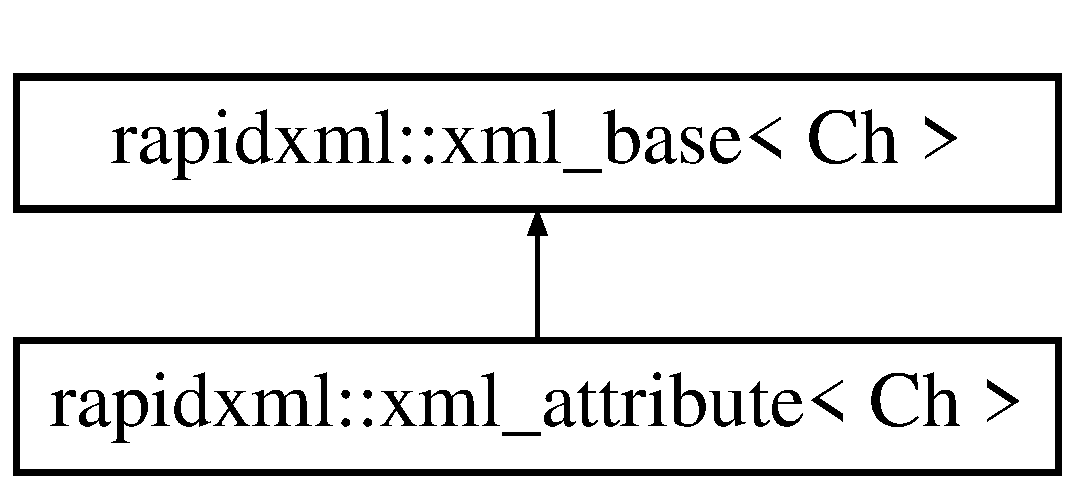
\includegraphics[height=2.000000cm]{classrapidxml_1_1xml__attribute}
\end{center}
\end{figure}
\subsection*{Public Member Functions}
\begin{DoxyCompactItemize}
\item 
\hyperlink{classrapidxml_1_1xml__attribute_a26be291103917d3e8de110d46dd83816}{xml\+\_\+attribute} ()
\item 
\hyperlink{classrapidxml_1_1xml__document}{xml\+\_\+document}$<$ Ch $>$ $\ast$ \hyperlink{classrapidxml_1_1xml__attribute_a8b6d31d899e27f01bde35b53d98496ec}{document} () const 
\item 
\hyperlink{classrapidxml_1_1xml__attribute}{xml\+\_\+attribute}$<$ Ch $>$ $\ast$ \hyperlink{classrapidxml_1_1xml__attribute_ae3547cc30b201fd6d7b98c04dda26f89}{previous\+\_\+attribute} (const Ch $\ast$\hyperlink{classrapidxml_1_1xml__base_a9a09739310469995db078ebd0da3ed45}{name}=0, std\+::size\+\_\+t \hyperlink{classrapidxml_1_1xml__base_a7e7f98b3d01e1eab8dc1ca69aad9af84}{name\+\_\+size}=0, bool case\+\_\+sensitive=true) const 
\item 
\hyperlink{classrapidxml_1_1xml__attribute}{xml\+\_\+attribute}$<$ Ch $>$ $\ast$ \hyperlink{classrapidxml_1_1xml__attribute_a56c08d7c96203286c889a43849328a86}{next\+\_\+attribute} (const Ch $\ast$\hyperlink{classrapidxml_1_1xml__base_a9a09739310469995db078ebd0da3ed45}{name}=0, std\+::size\+\_\+t \hyperlink{classrapidxml_1_1xml__base_a7e7f98b3d01e1eab8dc1ca69aad9af84}{name\+\_\+size}=0, bool case\+\_\+sensitive=true) const 
\item 
Ch $\ast$ \hyperlink{classrapidxml_1_1xml__base_a9a09739310469995db078ebd0da3ed45}{name} () const 
\item 
void \hyperlink{classrapidxml_1_1xml__base_ae55060ae958c6e6465d6c8db852ec6ce}{name} (const Ch $\ast$name, std\+::size\+\_\+t size)
\item 
void \hyperlink{classrapidxml_1_1xml__base_a4611ddc82ac83a527c65606600eb2a0d}{name} (const Ch $\ast$name)
\item 
std\+::size\+\_\+t \hyperlink{classrapidxml_1_1xml__base_a7e7f98b3d01e1eab8dc1ca69aad9af84}{name\+\_\+size} () const 
\item 
Ch $\ast$ \hyperlink{classrapidxml_1_1xml__base_adcdaccff61c665f039d9344e447b7445}{value} () const 
\item 
void \hyperlink{classrapidxml_1_1xml__base_a3b183c2db7022a6d30494dd2f0ac11e9}{value} (const Ch $\ast$value, std\+::size\+\_\+t size)
\item 
void \hyperlink{classrapidxml_1_1xml__base_a81e63ec4bfd2d7ef0a6c2ed49be6e623}{value} (const Ch $\ast$value)
\item 
std\+::size\+\_\+t \hyperlink{classrapidxml_1_1xml__base_a9fcf201ed0915ac18dd43b0b5dcfaf32}{value\+\_\+size} () const 
\item 
\hyperlink{classrapidxml_1_1xml__node}{xml\+\_\+node}$<$ Ch $>$ $\ast$ \hyperlink{classrapidxml_1_1xml__base_a7f31ae930f93852830234db1ae59c4c4}{parent} () const 
\end{DoxyCompactItemize}
\subsection*{Static Protected Member Functions}
\begin{DoxyCompactItemize}
\item 
static Ch $\ast$ \hyperlink{classrapidxml_1_1xml__base_ad96ff6b1e41dab3ff60b9bc4df769a75}{nullstr} ()
\end{DoxyCompactItemize}
\subsection*{Protected Attributes}
\begin{DoxyCompactItemize}
\item 
Ch $\ast$ \hyperlink{classrapidxml_1_1xml__base_afd9851ed43e14619db0d7075ef8e9e8a}{m\+\_\+name}
\item 
Ch $\ast$ \hyperlink{classrapidxml_1_1xml__base_a278a1ea63b0b70219b946cec47fa00ea}{m\+\_\+value}
\item 
std\+::size\+\_\+t \hyperlink{classrapidxml_1_1xml__base_a5a8c76a7274b4180213796422c4df76f}{m\+\_\+name\+\_\+size}
\item 
std\+::size\+\_\+t \hyperlink{classrapidxml_1_1xml__base_aa3a49d8ceddb8a8d7edb773a2226b89c}{m\+\_\+value\+\_\+size}
\item 
\hyperlink{classrapidxml_1_1xml__node}{xml\+\_\+node}$<$ Ch $>$ $\ast$ \hyperlink{classrapidxml_1_1xml__base_a90d5f660f078f66563fd7b2d8387ccb0}{m\+\_\+parent}
\end{DoxyCompactItemize}
\subsection*{Private Attributes}
\begin{DoxyCompactItemize}
\item 
\hyperlink{classrapidxml_1_1xml__attribute}{xml\+\_\+attribute}$<$ Ch $>$ $\ast$ \hyperlink{classrapidxml_1_1xml__attribute_a204438287a5ad384405584726a1d8559}{m\+\_\+prev\+\_\+attribute}
\item 
\hyperlink{classrapidxml_1_1xml__attribute}{xml\+\_\+attribute}$<$ Ch $>$ $\ast$ \hyperlink{classrapidxml_1_1xml__attribute_a3254e4b040a9b71c6b6d1c27ec03352a}{m\+\_\+next\+\_\+attribute}
\end{DoxyCompactItemize}
\subsection*{Friends}
\begin{DoxyCompactItemize}
\item 
class \hyperlink{classrapidxml_1_1xml__attribute_aa7e464ce3fe512598ff8dda47291941f}{xml\+\_\+node$<$ Ch $>$}
\end{DoxyCompactItemize}


\subsection{Detailed Description}
\subsubsection*{template$<$class Ch = char$>$class rapidxml\+::xml\+\_\+attribute$<$ Ch $>$}

Class representing attribute node of X\+M\+L document. Each attribute has name and value strings, which are available through \hyperlink{classrapidxml_1_1xml__base_a9a09739310469995db078ebd0da3ed45}{name()} and \hyperlink{classrapidxml_1_1xml__base_adcdaccff61c665f039d9344e447b7445}{value()} functions (inherited from \hyperlink{classrapidxml_1_1xml__base}{xml\+\_\+base}). Note that after parse, both name and value of attribute will point to interior of source text used for parsing. Thus, this text must persist in memory for the lifetime of attribute. 
\begin{DoxyParams}{Parameters}
{\em Ch} & Character type to use. \\
\hline
\end{DoxyParams}


\subsection{Constructor \& Destructor Documentation}
\hypertarget{classrapidxml_1_1xml__attribute_a26be291103917d3e8de110d46dd83816}{}\index{rapidxml\+::xml\+\_\+attribute@{rapidxml\+::xml\+\_\+attribute}!xml\+\_\+attribute@{xml\+\_\+attribute}}
\index{xml\+\_\+attribute@{xml\+\_\+attribute}!rapidxml\+::xml\+\_\+attribute@{rapidxml\+::xml\+\_\+attribute}}
\subsubsection[{xml\+\_\+attribute}]{\setlength{\rightskip}{0pt plus 5cm}template$<$class Ch = char$>$ {\bf rapidxml\+::xml\+\_\+attribute}$<$ Ch $>$\+::{\bf xml\+\_\+attribute} (
\begin{DoxyParamCaption}
{}
\end{DoxyParamCaption}
)\hspace{0.3cm}{\ttfamily [inline]}}\label{classrapidxml_1_1xml__attribute_a26be291103917d3e8de110d46dd83816}
Constructs an empty attribute with the specified type. Consider using \hyperlink{classrapidxml_1_1memory__pool}{memory\+\_\+pool} of appropriate \hyperlink{classrapidxml_1_1xml__document}{xml\+\_\+document} if allocating attributes manually. 

\subsection{Member Function Documentation}
\hypertarget{classrapidxml_1_1xml__attribute_a8b6d31d899e27f01bde35b53d98496ec}{}\index{rapidxml\+::xml\+\_\+attribute@{rapidxml\+::xml\+\_\+attribute}!document@{document}}
\index{document@{document}!rapidxml\+::xml\+\_\+attribute@{rapidxml\+::xml\+\_\+attribute}}
\subsubsection[{document}]{\setlength{\rightskip}{0pt plus 5cm}template$<$class Ch = char$>$ {\bf xml\+\_\+document}$<$Ch$>$$\ast$ {\bf rapidxml\+::xml\+\_\+attribute}$<$ Ch $>$\+::document (
\begin{DoxyParamCaption}
{}
\end{DoxyParamCaption}
) const\hspace{0.3cm}{\ttfamily [inline]}}\label{classrapidxml_1_1xml__attribute_a8b6d31d899e27f01bde35b53d98496ec}
Gets document of which attribute is a child. \begin{DoxyReturn}{Returns}
Pointer to document that contains this attribute, or 0 if there is no parent document. 
\end{DoxyReturn}
\hypertarget{classrapidxml_1_1xml__base_a9a09739310469995db078ebd0da3ed45}{}\index{rapidxml\+::xml\+\_\+attribute@{rapidxml\+::xml\+\_\+attribute}!name@{name}}
\index{name@{name}!rapidxml\+::xml\+\_\+attribute@{rapidxml\+::xml\+\_\+attribute}}
\subsubsection[{name}]{\setlength{\rightskip}{0pt plus 5cm}template$<$class Ch  = char$>$ Ch$\ast$ {\bf rapidxml\+::xml\+\_\+base}$<$ Ch $>$\+::name (
\begin{DoxyParamCaption}
{}
\end{DoxyParamCaption}
) const\hspace{0.3cm}{\ttfamily [inline]}, {\ttfamily [inherited]}}\label{classrapidxml_1_1xml__base_a9a09739310469995db078ebd0da3ed45}
Gets name of the node. Interpretation of name depends on type of node. Note that name will not be zero-\/terminated if \hyperlink{namespacerapidxml_af3fc88ba6bee33482a2db81b1da36ea1}{rapidxml\+::parse\+\_\+no\+\_\+string\+\_\+terminators} option was selected during parse. ~\newline
~\newline
 Use \hyperlink{classrapidxml_1_1xml__base_a7e7f98b3d01e1eab8dc1ca69aad9af84}{name\+\_\+size()} function to determine length of the name. \begin{DoxyReturn}{Returns}
Name of node, or empty string if node has no name. 
\end{DoxyReturn}
\hypertarget{classrapidxml_1_1xml__base_ae55060ae958c6e6465d6c8db852ec6ce}{}\index{rapidxml\+::xml\+\_\+attribute@{rapidxml\+::xml\+\_\+attribute}!name@{name}}
\index{name@{name}!rapidxml\+::xml\+\_\+attribute@{rapidxml\+::xml\+\_\+attribute}}
\subsubsection[{name}]{\setlength{\rightskip}{0pt plus 5cm}template$<$class Ch  = char$>$ void {\bf rapidxml\+::xml\+\_\+base}$<$ Ch $>$\+::name (
\begin{DoxyParamCaption}
\item[{const Ch $\ast$}]{name, }
\item[{std\+::size\+\_\+t}]{size}
\end{DoxyParamCaption}
)\hspace{0.3cm}{\ttfamily [inline]}, {\ttfamily [inherited]}}\label{classrapidxml_1_1xml__base_ae55060ae958c6e6465d6c8db852ec6ce}
Sets name of node to a non zero-\/terminated string. See ownership\+\_\+of\+\_\+strings. ~\newline
~\newline
 Note that node does not own its name or value, it only stores a pointer to it. It will not delete or otherwise free the pointer on destruction. It is reponsibility of the user to properly manage lifetime of the string. The easiest way to achieve it is to use \hyperlink{classrapidxml_1_1memory__pool}{memory\+\_\+pool} of the document to allocate the string -\/ on destruction of the document the string will be automatically freed. ~\newline
~\newline
 Size of name must be specified separately, because name does not have to be zero terminated. Use \hyperlink{classrapidxml_1_1xml__base_a4611ddc82ac83a527c65606600eb2a0d}{name(const Ch $\ast$)} function to have the length automatically calculated (string must be zero terminated). 
\begin{DoxyParams}{Parameters}
{\em name} & Name of node to set. Does not have to be zero terminated. \\
\hline
{\em size} & Size of name, in characters. This does not include zero terminator, if one is present. \\
\hline
\end{DoxyParams}
\hypertarget{classrapidxml_1_1xml__base_a4611ddc82ac83a527c65606600eb2a0d}{}\index{rapidxml\+::xml\+\_\+attribute@{rapidxml\+::xml\+\_\+attribute}!name@{name}}
\index{name@{name}!rapidxml\+::xml\+\_\+attribute@{rapidxml\+::xml\+\_\+attribute}}
\subsubsection[{name}]{\setlength{\rightskip}{0pt plus 5cm}template$<$class Ch  = char$>$ void {\bf rapidxml\+::xml\+\_\+base}$<$ Ch $>$\+::name (
\begin{DoxyParamCaption}
\item[{const Ch $\ast$}]{name}
\end{DoxyParamCaption}
)\hspace{0.3cm}{\ttfamily [inline]}, {\ttfamily [inherited]}}\label{classrapidxml_1_1xml__base_a4611ddc82ac83a527c65606600eb2a0d}
Sets name of node to a zero-\/terminated string. See also ownership\+\_\+of\+\_\+strings and \hyperlink{classrapidxml_1_1xml__base_ae55060ae958c6e6465d6c8db852ec6ce}{xml\+\_\+node\+::name(const Ch $\ast$, std\+::size\+\_\+t)}. 
\begin{DoxyParams}{Parameters}
{\em name} & Name of node to set. Must be zero terminated. \\
\hline
\end{DoxyParams}
\hypertarget{classrapidxml_1_1xml__base_a7e7f98b3d01e1eab8dc1ca69aad9af84}{}\index{rapidxml\+::xml\+\_\+attribute@{rapidxml\+::xml\+\_\+attribute}!name\+\_\+size@{name\+\_\+size}}
\index{name\+\_\+size@{name\+\_\+size}!rapidxml\+::xml\+\_\+attribute@{rapidxml\+::xml\+\_\+attribute}}
\subsubsection[{name\+\_\+size}]{\setlength{\rightskip}{0pt plus 5cm}template$<$class Ch  = char$>$ std\+::size\+\_\+t {\bf rapidxml\+::xml\+\_\+base}$<$ Ch $>$\+::name\+\_\+size (
\begin{DoxyParamCaption}
{}
\end{DoxyParamCaption}
) const\hspace{0.3cm}{\ttfamily [inline]}, {\ttfamily [inherited]}}\label{classrapidxml_1_1xml__base_a7e7f98b3d01e1eab8dc1ca69aad9af84}
Gets size of node name, not including terminator character. This function works correctly irrespective of whether name is or is not zero terminated. \begin{DoxyReturn}{Returns}
Size of node name, in characters. 
\end{DoxyReturn}
\hypertarget{classrapidxml_1_1xml__attribute_a56c08d7c96203286c889a43849328a86}{}\index{rapidxml\+::xml\+\_\+attribute@{rapidxml\+::xml\+\_\+attribute}!next\+\_\+attribute@{next\+\_\+attribute}}
\index{next\+\_\+attribute@{next\+\_\+attribute}!rapidxml\+::xml\+\_\+attribute@{rapidxml\+::xml\+\_\+attribute}}
\subsubsection[{next\+\_\+attribute}]{\setlength{\rightskip}{0pt plus 5cm}template$<$class Ch = char$>$ {\bf xml\+\_\+attribute}$<$Ch$>$$\ast$ {\bf rapidxml\+::xml\+\_\+attribute}$<$ Ch $>$\+::next\+\_\+attribute (
\begin{DoxyParamCaption}
\item[{const Ch $\ast$}]{name = {\ttfamily 0}, }
\item[{std\+::size\+\_\+t}]{name\+\_\+size = {\ttfamily 0}, }
\item[{bool}]{case\+\_\+sensitive = {\ttfamily true}}
\end{DoxyParamCaption}
) const\hspace{0.3cm}{\ttfamily [inline]}}\label{classrapidxml_1_1xml__attribute_a56c08d7c96203286c889a43849328a86}
Gets next attribute, optionally matching attribute name. 
\begin{DoxyParams}{Parameters}
{\em name} & Name of attribute to find, or 0 to return next attribute regardless of its name; this string doesn\textquotesingle{}t have to be zero-\/terminated if name\+\_\+size is non-\/zero \\
\hline
{\em name\+\_\+size} & Size of name, in characters, or 0 to have size calculated automatically from string \\
\hline
{\em case\+\_\+sensitive} & Should name comparison be case-\/sensitive; non case-\/sensitive comparison works properly only for A\+S\+C\+I\+I characters \\
\hline
\end{DoxyParams}
\begin{DoxyReturn}{Returns}
Pointer to found attribute, or 0 if not found. 
\end{DoxyReturn}
\hypertarget{classrapidxml_1_1xml__base_ad96ff6b1e41dab3ff60b9bc4df769a75}{}\index{rapidxml\+::xml\+\_\+attribute@{rapidxml\+::xml\+\_\+attribute}!nullstr@{nullstr}}
\index{nullstr@{nullstr}!rapidxml\+::xml\+\_\+attribute@{rapidxml\+::xml\+\_\+attribute}}
\subsubsection[{nullstr}]{\setlength{\rightskip}{0pt plus 5cm}template$<$class Ch  = char$>$ static Ch$\ast$ {\bf rapidxml\+::xml\+\_\+base}$<$ Ch $>$\+::nullstr (
\begin{DoxyParamCaption}
{}
\end{DoxyParamCaption}
)\hspace{0.3cm}{\ttfamily [inline]}, {\ttfamily [static]}, {\ttfamily [protected]}, {\ttfamily [inherited]}}\label{classrapidxml_1_1xml__base_ad96ff6b1e41dab3ff60b9bc4df769a75}
\hypertarget{classrapidxml_1_1xml__base_a7f31ae930f93852830234db1ae59c4c4}{}\index{rapidxml\+::xml\+\_\+attribute@{rapidxml\+::xml\+\_\+attribute}!parent@{parent}}
\index{parent@{parent}!rapidxml\+::xml\+\_\+attribute@{rapidxml\+::xml\+\_\+attribute}}
\subsubsection[{parent}]{\setlength{\rightskip}{0pt plus 5cm}template$<$class Ch  = char$>$ {\bf xml\+\_\+node}$<$Ch$>$$\ast$ {\bf rapidxml\+::xml\+\_\+base}$<$ Ch $>$\+::parent (
\begin{DoxyParamCaption}
{}
\end{DoxyParamCaption}
) const\hspace{0.3cm}{\ttfamily [inline]}, {\ttfamily [inherited]}}\label{classrapidxml_1_1xml__base_a7f31ae930f93852830234db1ae59c4c4}
Gets node parent. \begin{DoxyReturn}{Returns}
Pointer to parent node, or 0 if there is no parent. 
\end{DoxyReturn}
\hypertarget{classrapidxml_1_1xml__attribute_ae3547cc30b201fd6d7b98c04dda26f89}{}\index{rapidxml\+::xml\+\_\+attribute@{rapidxml\+::xml\+\_\+attribute}!previous\+\_\+attribute@{previous\+\_\+attribute}}
\index{previous\+\_\+attribute@{previous\+\_\+attribute}!rapidxml\+::xml\+\_\+attribute@{rapidxml\+::xml\+\_\+attribute}}
\subsubsection[{previous\+\_\+attribute}]{\setlength{\rightskip}{0pt plus 5cm}template$<$class Ch = char$>$ {\bf xml\+\_\+attribute}$<$Ch$>$$\ast$ {\bf rapidxml\+::xml\+\_\+attribute}$<$ Ch $>$\+::previous\+\_\+attribute (
\begin{DoxyParamCaption}
\item[{const Ch $\ast$}]{name = {\ttfamily 0}, }
\item[{std\+::size\+\_\+t}]{name\+\_\+size = {\ttfamily 0}, }
\item[{bool}]{case\+\_\+sensitive = {\ttfamily true}}
\end{DoxyParamCaption}
) const\hspace{0.3cm}{\ttfamily [inline]}}\label{classrapidxml_1_1xml__attribute_ae3547cc30b201fd6d7b98c04dda26f89}
Gets previous attribute, optionally matching attribute name. 
\begin{DoxyParams}{Parameters}
{\em name} & Name of attribute to find, or 0 to return previous attribute regardless of its name; this string doesn\textquotesingle{}t have to be zero-\/terminated if name\+\_\+size is non-\/zero \\
\hline
{\em name\+\_\+size} & Size of name, in characters, or 0 to have size calculated automatically from string \\
\hline
{\em case\+\_\+sensitive} & Should name comparison be case-\/sensitive; non case-\/sensitive comparison works properly only for A\+S\+C\+I\+I characters \\
\hline
\end{DoxyParams}
\begin{DoxyReturn}{Returns}
Pointer to found attribute, or 0 if not found. 
\end{DoxyReturn}
\hypertarget{classrapidxml_1_1xml__base_adcdaccff61c665f039d9344e447b7445}{}\index{rapidxml\+::xml\+\_\+attribute@{rapidxml\+::xml\+\_\+attribute}!value@{value}}
\index{value@{value}!rapidxml\+::xml\+\_\+attribute@{rapidxml\+::xml\+\_\+attribute}}
\subsubsection[{value}]{\setlength{\rightskip}{0pt plus 5cm}template$<$class Ch  = char$>$ Ch$\ast$ {\bf rapidxml\+::xml\+\_\+base}$<$ Ch $>$\+::value (
\begin{DoxyParamCaption}
{}
\end{DoxyParamCaption}
) const\hspace{0.3cm}{\ttfamily [inline]}, {\ttfamily [inherited]}}\label{classrapidxml_1_1xml__base_adcdaccff61c665f039d9344e447b7445}
Gets value of node. Interpretation of value depends on type of node. Note that value will not be zero-\/terminated if \hyperlink{namespacerapidxml_af3fc88ba6bee33482a2db81b1da36ea1}{rapidxml\+::parse\+\_\+no\+\_\+string\+\_\+terminators} option was selected during parse. ~\newline
~\newline
 Use \hyperlink{classrapidxml_1_1xml__base_a9fcf201ed0915ac18dd43b0b5dcfaf32}{value\+\_\+size()} function to determine length of the value. \begin{DoxyReturn}{Returns}
Value of node, or empty string if node has no value. 
\end{DoxyReturn}
\hypertarget{classrapidxml_1_1xml__base_a3b183c2db7022a6d30494dd2f0ac11e9}{}\index{rapidxml\+::xml\+\_\+attribute@{rapidxml\+::xml\+\_\+attribute}!value@{value}}
\index{value@{value}!rapidxml\+::xml\+\_\+attribute@{rapidxml\+::xml\+\_\+attribute}}
\subsubsection[{value}]{\setlength{\rightskip}{0pt plus 5cm}template$<$class Ch  = char$>$ void {\bf rapidxml\+::xml\+\_\+base}$<$ Ch $>$\+::value (
\begin{DoxyParamCaption}
\item[{const Ch $\ast$}]{value, }
\item[{std\+::size\+\_\+t}]{size}
\end{DoxyParamCaption}
)\hspace{0.3cm}{\ttfamily [inline]}, {\ttfamily [inherited]}}\label{classrapidxml_1_1xml__base_a3b183c2db7022a6d30494dd2f0ac11e9}
Sets value of node to a non zero-\/terminated string. See ownership\+\_\+of\+\_\+strings. ~\newline
~\newline
 Note that node does not own its name or value, it only stores a pointer to it. It will not delete or otherwise free the pointer on destruction. It is reponsibility of the user to properly manage lifetime of the string. The easiest way to achieve it is to use \hyperlink{classrapidxml_1_1memory__pool}{memory\+\_\+pool} of the document to allocate the string -\/ on destruction of the document the string will be automatically freed. ~\newline
~\newline
 Size of value must be specified separately, because it does not have to be zero terminated. Use \hyperlink{classrapidxml_1_1xml__base_a81e63ec4bfd2d7ef0a6c2ed49be6e623}{value(const Ch $\ast$)} function to have the length automatically calculated (string must be zero terminated). ~\newline
~\newline
 If an element has a child node of type node\+\_\+data, it will take precedence over element value when printing. If you want to manipulate data of elements using values, use parser flag \hyperlink{namespacerapidxml_ac2d21ef14a4e8936b94aca5d38b1a74d}{rapidxml\+::parse\+\_\+no\+\_\+data\+\_\+nodes} to prevent creation of data nodes by the parser. 
\begin{DoxyParams}{Parameters}
{\em value} & value of node to set. Does not have to be zero terminated. \\
\hline
{\em size} & Size of value, in characters. This does not include zero terminator, if one is present. \\
\hline
\end{DoxyParams}
\hypertarget{classrapidxml_1_1xml__base_a81e63ec4bfd2d7ef0a6c2ed49be6e623}{}\index{rapidxml\+::xml\+\_\+attribute@{rapidxml\+::xml\+\_\+attribute}!value@{value}}
\index{value@{value}!rapidxml\+::xml\+\_\+attribute@{rapidxml\+::xml\+\_\+attribute}}
\subsubsection[{value}]{\setlength{\rightskip}{0pt plus 5cm}template$<$class Ch  = char$>$ void {\bf rapidxml\+::xml\+\_\+base}$<$ Ch $>$\+::value (
\begin{DoxyParamCaption}
\item[{const Ch $\ast$}]{value}
\end{DoxyParamCaption}
)\hspace{0.3cm}{\ttfamily [inline]}, {\ttfamily [inherited]}}\label{classrapidxml_1_1xml__base_a81e63ec4bfd2d7ef0a6c2ed49be6e623}
Sets value of node to a zero-\/terminated string. See also ownership\+\_\+of\+\_\+strings and \hyperlink{classrapidxml_1_1xml__base_a3b183c2db7022a6d30494dd2f0ac11e9}{xml\+\_\+node\+::value(const Ch $\ast$, std\+::size\+\_\+t)}. 
\begin{DoxyParams}{Parameters}
{\em value} & Vame of node to set. Must be zero terminated. \\
\hline
\end{DoxyParams}
\hypertarget{classrapidxml_1_1xml__base_a9fcf201ed0915ac18dd43b0b5dcfaf32}{}\index{rapidxml\+::xml\+\_\+attribute@{rapidxml\+::xml\+\_\+attribute}!value\+\_\+size@{value\+\_\+size}}
\index{value\+\_\+size@{value\+\_\+size}!rapidxml\+::xml\+\_\+attribute@{rapidxml\+::xml\+\_\+attribute}}
\subsubsection[{value\+\_\+size}]{\setlength{\rightskip}{0pt plus 5cm}template$<$class Ch  = char$>$ std\+::size\+\_\+t {\bf rapidxml\+::xml\+\_\+base}$<$ Ch $>$\+::value\+\_\+size (
\begin{DoxyParamCaption}
{}
\end{DoxyParamCaption}
) const\hspace{0.3cm}{\ttfamily [inline]}, {\ttfamily [inherited]}}\label{classrapidxml_1_1xml__base_a9fcf201ed0915ac18dd43b0b5dcfaf32}
Gets size of node value, not including terminator character. This function works correctly irrespective of whether value is or is not zero terminated. \begin{DoxyReturn}{Returns}
Size of node value, in characters. 
\end{DoxyReturn}


\subsection{Friends And Related Function Documentation}
\hypertarget{classrapidxml_1_1xml__attribute_aa7e464ce3fe512598ff8dda47291941f}{}\index{rapidxml\+::xml\+\_\+attribute@{rapidxml\+::xml\+\_\+attribute}!xml\+\_\+node$<$ Ch $>$@{xml\+\_\+node$<$ Ch $>$}}
\index{xml\+\_\+node$<$ Ch $>$@{xml\+\_\+node$<$ Ch $>$}!rapidxml\+::xml\+\_\+attribute@{rapidxml\+::xml\+\_\+attribute}}
\subsubsection[{xml\+\_\+node$<$ Ch $>$}]{\setlength{\rightskip}{0pt plus 5cm}template$<$class Ch = char$>$ friend class {\bf xml\+\_\+node}$<$ Ch $>$\hspace{0.3cm}{\ttfamily [friend]}}\label{classrapidxml_1_1xml__attribute_aa7e464ce3fe512598ff8dda47291941f}


\subsection{Member Data Documentation}
\hypertarget{classrapidxml_1_1xml__base_afd9851ed43e14619db0d7075ef8e9e8a}{}\index{rapidxml\+::xml\+\_\+attribute@{rapidxml\+::xml\+\_\+attribute}!m\+\_\+name@{m\+\_\+name}}
\index{m\+\_\+name@{m\+\_\+name}!rapidxml\+::xml\+\_\+attribute@{rapidxml\+::xml\+\_\+attribute}}
\subsubsection[{m\+\_\+name}]{\setlength{\rightskip}{0pt plus 5cm}template$<$class Ch  = char$>$ Ch$\ast$ {\bf rapidxml\+::xml\+\_\+base}$<$ Ch $>$\+::m\+\_\+name\hspace{0.3cm}{\ttfamily [protected]}, {\ttfamily [inherited]}}\label{classrapidxml_1_1xml__base_afd9851ed43e14619db0d7075ef8e9e8a}
\hypertarget{classrapidxml_1_1xml__base_a5a8c76a7274b4180213796422c4df76f}{}\index{rapidxml\+::xml\+\_\+attribute@{rapidxml\+::xml\+\_\+attribute}!m\+\_\+name\+\_\+size@{m\+\_\+name\+\_\+size}}
\index{m\+\_\+name\+\_\+size@{m\+\_\+name\+\_\+size}!rapidxml\+::xml\+\_\+attribute@{rapidxml\+::xml\+\_\+attribute}}
\subsubsection[{m\+\_\+name\+\_\+size}]{\setlength{\rightskip}{0pt plus 5cm}template$<$class Ch  = char$>$ std\+::size\+\_\+t {\bf rapidxml\+::xml\+\_\+base}$<$ Ch $>$\+::m\+\_\+name\+\_\+size\hspace{0.3cm}{\ttfamily [protected]}, {\ttfamily [inherited]}}\label{classrapidxml_1_1xml__base_a5a8c76a7274b4180213796422c4df76f}
\hypertarget{classrapidxml_1_1xml__attribute_a3254e4b040a9b71c6b6d1c27ec03352a}{}\index{rapidxml\+::xml\+\_\+attribute@{rapidxml\+::xml\+\_\+attribute}!m\+\_\+next\+\_\+attribute@{m\+\_\+next\+\_\+attribute}}
\index{m\+\_\+next\+\_\+attribute@{m\+\_\+next\+\_\+attribute}!rapidxml\+::xml\+\_\+attribute@{rapidxml\+::xml\+\_\+attribute}}
\subsubsection[{m\+\_\+next\+\_\+attribute}]{\setlength{\rightskip}{0pt plus 5cm}template$<$class Ch = char$>$ {\bf xml\+\_\+attribute}$<$Ch$>$$\ast$ {\bf rapidxml\+::xml\+\_\+attribute}$<$ Ch $>$\+::m\+\_\+next\+\_\+attribute\hspace{0.3cm}{\ttfamily [private]}}\label{classrapidxml_1_1xml__attribute_a3254e4b040a9b71c6b6d1c27ec03352a}
\hypertarget{classrapidxml_1_1xml__base_a90d5f660f078f66563fd7b2d8387ccb0}{}\index{rapidxml\+::xml\+\_\+attribute@{rapidxml\+::xml\+\_\+attribute}!m\+\_\+parent@{m\+\_\+parent}}
\index{m\+\_\+parent@{m\+\_\+parent}!rapidxml\+::xml\+\_\+attribute@{rapidxml\+::xml\+\_\+attribute}}
\subsubsection[{m\+\_\+parent}]{\setlength{\rightskip}{0pt plus 5cm}template$<$class Ch  = char$>$ {\bf xml\+\_\+node}$<$Ch$>$$\ast$ {\bf rapidxml\+::xml\+\_\+base}$<$ Ch $>$\+::m\+\_\+parent\hspace{0.3cm}{\ttfamily [protected]}, {\ttfamily [inherited]}}\label{classrapidxml_1_1xml__base_a90d5f660f078f66563fd7b2d8387ccb0}
\hypertarget{classrapidxml_1_1xml__attribute_a204438287a5ad384405584726a1d8559}{}\index{rapidxml\+::xml\+\_\+attribute@{rapidxml\+::xml\+\_\+attribute}!m\+\_\+prev\+\_\+attribute@{m\+\_\+prev\+\_\+attribute}}
\index{m\+\_\+prev\+\_\+attribute@{m\+\_\+prev\+\_\+attribute}!rapidxml\+::xml\+\_\+attribute@{rapidxml\+::xml\+\_\+attribute}}
\subsubsection[{m\+\_\+prev\+\_\+attribute}]{\setlength{\rightskip}{0pt plus 5cm}template$<$class Ch = char$>$ {\bf xml\+\_\+attribute}$<$Ch$>$$\ast$ {\bf rapidxml\+::xml\+\_\+attribute}$<$ Ch $>$\+::m\+\_\+prev\+\_\+attribute\hspace{0.3cm}{\ttfamily [private]}}\label{classrapidxml_1_1xml__attribute_a204438287a5ad384405584726a1d8559}
\hypertarget{classrapidxml_1_1xml__base_a278a1ea63b0b70219b946cec47fa00ea}{}\index{rapidxml\+::xml\+\_\+attribute@{rapidxml\+::xml\+\_\+attribute}!m\+\_\+value@{m\+\_\+value}}
\index{m\+\_\+value@{m\+\_\+value}!rapidxml\+::xml\+\_\+attribute@{rapidxml\+::xml\+\_\+attribute}}
\subsubsection[{m\+\_\+value}]{\setlength{\rightskip}{0pt plus 5cm}template$<$class Ch  = char$>$ Ch$\ast$ {\bf rapidxml\+::xml\+\_\+base}$<$ Ch $>$\+::m\+\_\+value\hspace{0.3cm}{\ttfamily [protected]}, {\ttfamily [inherited]}}\label{classrapidxml_1_1xml__base_a278a1ea63b0b70219b946cec47fa00ea}
\hypertarget{classrapidxml_1_1xml__base_aa3a49d8ceddb8a8d7edb773a2226b89c}{}\index{rapidxml\+::xml\+\_\+attribute@{rapidxml\+::xml\+\_\+attribute}!m\+\_\+value\+\_\+size@{m\+\_\+value\+\_\+size}}
\index{m\+\_\+value\+\_\+size@{m\+\_\+value\+\_\+size}!rapidxml\+::xml\+\_\+attribute@{rapidxml\+::xml\+\_\+attribute}}
\subsubsection[{m\+\_\+value\+\_\+size}]{\setlength{\rightskip}{0pt plus 5cm}template$<$class Ch  = char$>$ std\+::size\+\_\+t {\bf rapidxml\+::xml\+\_\+base}$<$ Ch $>$\+::m\+\_\+value\+\_\+size\hspace{0.3cm}{\ttfamily [protected]}, {\ttfamily [inherited]}}\label{classrapidxml_1_1xml__base_aa3a49d8ceddb8a8d7edb773a2226b89c}


The documentation for this class was generated from the following file\+:\begin{DoxyCompactItemize}
\item 
\hyperlink{rapidxml_8hpp}{rapidxml.\+hpp}\end{DoxyCompactItemize}

\hypertarget{classrapidxml_1_1xml__base}{}\section{rapidxml\+:\+:xml\+\_\+base$<$ Ch $>$ Class Template Reference}
\label{classrapidxml_1_1xml__base}\index{rapidxml\+::xml\+\_\+base$<$ Ch $>$@{rapidxml\+::xml\+\_\+base$<$ Ch $>$}}


{\ttfamily \#include $<$rapidxml.\+hpp$>$}

Inheritance diagram for rapidxml\+:\+:xml\+\_\+base$<$ Ch $>$\+:\begin{figure}[H]
\begin{center}
\leavevmode
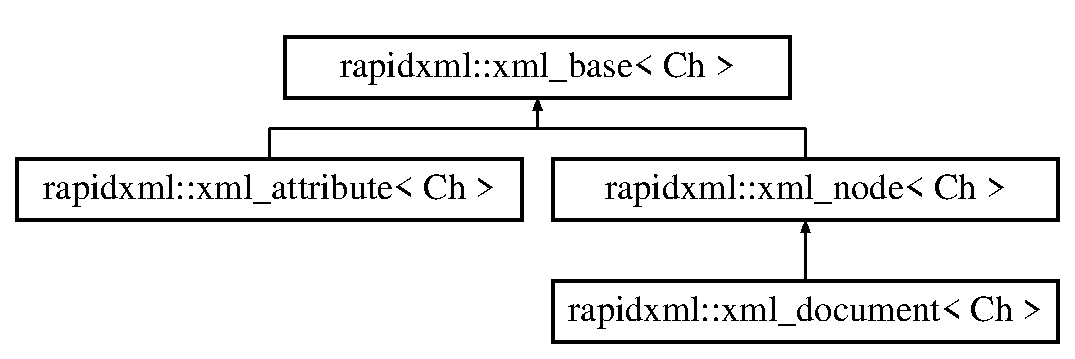
\includegraphics[height=3.000000cm]{classrapidxml_1_1xml__base}
\end{center}
\end{figure}
\subsection*{Public Member Functions}
\begin{DoxyCompactItemize}
\item 
\hyperlink{classrapidxml_1_1xml__base_a23e7f7aac02d17a0a01afb597e4b966b}{xml\+\_\+base} ()
\item 
Ch $\ast$ \hyperlink{classrapidxml_1_1xml__base_a9a09739310469995db078ebd0da3ed45}{name} () const 
\item 
std\+::size\+\_\+t \hyperlink{classrapidxml_1_1xml__base_a7e7f98b3d01e1eab8dc1ca69aad9af84}{name\+\_\+size} () const 
\item 
Ch $\ast$ \hyperlink{classrapidxml_1_1xml__base_adcdaccff61c665f039d9344e447b7445}{value} () const 
\item 
std\+::size\+\_\+t \hyperlink{classrapidxml_1_1xml__base_a9fcf201ed0915ac18dd43b0b5dcfaf32}{value\+\_\+size} () const 
\item 
void \hyperlink{classrapidxml_1_1xml__base_ae55060ae958c6e6465d6c8db852ec6ce}{name} (const Ch $\ast$name, std\+::size\+\_\+t size)
\item 
void \hyperlink{classrapidxml_1_1xml__base_a4611ddc82ac83a527c65606600eb2a0d}{name} (const Ch $\ast$name)
\item 
void \hyperlink{classrapidxml_1_1xml__base_a3b183c2db7022a6d30494dd2f0ac11e9}{value} (const Ch $\ast$value, std\+::size\+\_\+t size)
\item 
void \hyperlink{classrapidxml_1_1xml__base_a81e63ec4bfd2d7ef0a6c2ed49be6e623}{value} (const Ch $\ast$value)
\item 
\hyperlink{classrapidxml_1_1xml__node}{xml\+\_\+node}$<$ Ch $>$ $\ast$ \hyperlink{classrapidxml_1_1xml__base_a7f31ae930f93852830234db1ae59c4c4}{parent} () const 
\end{DoxyCompactItemize}
\subsection*{Static Protected Member Functions}
\begin{DoxyCompactItemize}
\item 
static Ch $\ast$ \hyperlink{classrapidxml_1_1xml__base_ad96ff6b1e41dab3ff60b9bc4df769a75}{nullstr} ()
\end{DoxyCompactItemize}
\subsection*{Protected Attributes}
\begin{DoxyCompactItemize}
\item 
Ch $\ast$ \hyperlink{classrapidxml_1_1xml__base_afd9851ed43e14619db0d7075ef8e9e8a}{m\+\_\+name}
\item 
Ch $\ast$ \hyperlink{classrapidxml_1_1xml__base_a278a1ea63b0b70219b946cec47fa00ea}{m\+\_\+value}
\item 
std\+::size\+\_\+t \hyperlink{classrapidxml_1_1xml__base_a5a8c76a7274b4180213796422c4df76f}{m\+\_\+name\+\_\+size}
\item 
std\+::size\+\_\+t \hyperlink{classrapidxml_1_1xml__base_aa3a49d8ceddb8a8d7edb773a2226b89c}{m\+\_\+value\+\_\+size}
\item 
\hyperlink{classrapidxml_1_1xml__node}{xml\+\_\+node}$<$ Ch $>$ $\ast$ \hyperlink{classrapidxml_1_1xml__base_a90d5f660f078f66563fd7b2d8387ccb0}{m\+\_\+parent}
\end{DoxyCompactItemize}


\subsection{Detailed Description}
\subsubsection*{template$<$class Ch = char$>$class rapidxml\+::xml\+\_\+base$<$ Ch $>$}

Base class for \hyperlink{classrapidxml_1_1xml__node}{xml\+\_\+node} and \hyperlink{classrapidxml_1_1xml__attribute}{xml\+\_\+attribute} implementing common functions\+: \hyperlink{classrapidxml_1_1xml__base_a9a09739310469995db078ebd0da3ed45}{name()}, \hyperlink{classrapidxml_1_1xml__base_a7e7f98b3d01e1eab8dc1ca69aad9af84}{name\+\_\+size()}, \hyperlink{classrapidxml_1_1xml__base_adcdaccff61c665f039d9344e447b7445}{value()}, \hyperlink{classrapidxml_1_1xml__base_a9fcf201ed0915ac18dd43b0b5dcfaf32}{value\+\_\+size()} and \hyperlink{classrapidxml_1_1xml__base_a7f31ae930f93852830234db1ae59c4c4}{parent()}. 
\begin{DoxyParams}{Parameters}
{\em Ch} & Character type to use \\
\hline
\end{DoxyParams}


\subsection{Constructor \& Destructor Documentation}
\hypertarget{classrapidxml_1_1xml__base_a23e7f7aac02d17a0a01afb597e4b966b}{}\index{rapidxml\+::xml\+\_\+base@{rapidxml\+::xml\+\_\+base}!xml\+\_\+base@{xml\+\_\+base}}
\index{xml\+\_\+base@{xml\+\_\+base}!rapidxml\+::xml\+\_\+base@{rapidxml\+::xml\+\_\+base}}
\subsubsection[{xml\+\_\+base}]{\setlength{\rightskip}{0pt plus 5cm}template$<$class Ch  = char$>$ {\bf rapidxml\+::xml\+\_\+base}$<$ Ch $>$\+::{\bf xml\+\_\+base} (
\begin{DoxyParamCaption}
{}
\end{DoxyParamCaption}
)\hspace{0.3cm}{\ttfamily [inline]}}\label{classrapidxml_1_1xml__base_a23e7f7aac02d17a0a01afb597e4b966b}


\subsection{Member Function Documentation}
\hypertarget{classrapidxml_1_1xml__base_a9a09739310469995db078ebd0da3ed45}{}\index{rapidxml\+::xml\+\_\+base@{rapidxml\+::xml\+\_\+base}!name@{name}}
\index{name@{name}!rapidxml\+::xml\+\_\+base@{rapidxml\+::xml\+\_\+base}}
\subsubsection[{name}]{\setlength{\rightskip}{0pt plus 5cm}template$<$class Ch  = char$>$ Ch$\ast$ {\bf rapidxml\+::xml\+\_\+base}$<$ Ch $>$\+::name (
\begin{DoxyParamCaption}
{}
\end{DoxyParamCaption}
) const\hspace{0.3cm}{\ttfamily [inline]}}\label{classrapidxml_1_1xml__base_a9a09739310469995db078ebd0da3ed45}
Gets name of the node. Interpretation of name depends on type of node. Note that name will not be zero-\/terminated if \hyperlink{namespacerapidxml_af3fc88ba6bee33482a2db81b1da36ea1}{rapidxml\+::parse\+\_\+no\+\_\+string\+\_\+terminators} option was selected during parse. ~\newline
~\newline
 Use \hyperlink{classrapidxml_1_1xml__base_a7e7f98b3d01e1eab8dc1ca69aad9af84}{name\+\_\+size()} function to determine length of the name. \begin{DoxyReturn}{Returns}
Name of node, or empty string if node has no name. 
\end{DoxyReturn}
\hypertarget{classrapidxml_1_1xml__base_ae55060ae958c6e6465d6c8db852ec6ce}{}\index{rapidxml\+::xml\+\_\+base@{rapidxml\+::xml\+\_\+base}!name@{name}}
\index{name@{name}!rapidxml\+::xml\+\_\+base@{rapidxml\+::xml\+\_\+base}}
\subsubsection[{name}]{\setlength{\rightskip}{0pt plus 5cm}template$<$class Ch  = char$>$ void {\bf rapidxml\+::xml\+\_\+base}$<$ Ch $>$\+::name (
\begin{DoxyParamCaption}
\item[{const Ch $\ast$}]{name, }
\item[{std\+::size\+\_\+t}]{size}
\end{DoxyParamCaption}
)\hspace{0.3cm}{\ttfamily [inline]}}\label{classrapidxml_1_1xml__base_ae55060ae958c6e6465d6c8db852ec6ce}
Sets name of node to a non zero-\/terminated string. See ownership\+\_\+of\+\_\+strings. ~\newline
~\newline
 Note that node does not own its name or value, it only stores a pointer to it. It will not delete or otherwise free the pointer on destruction. It is reponsibility of the user to properly manage lifetime of the string. The easiest way to achieve it is to use \hyperlink{classrapidxml_1_1memory__pool}{memory\+\_\+pool} of the document to allocate the string -\/ on destruction of the document the string will be automatically freed. ~\newline
~\newline
 Size of name must be specified separately, because name does not have to be zero terminated. Use \hyperlink{classrapidxml_1_1xml__base_a4611ddc82ac83a527c65606600eb2a0d}{name(const Ch $\ast$)} function to have the length automatically calculated (string must be zero terminated). 
\begin{DoxyParams}{Parameters}
{\em name} & Name of node to set. Does not have to be zero terminated. \\
\hline
{\em size} & Size of name, in characters. This does not include zero terminator, if one is present. \\
\hline
\end{DoxyParams}
\hypertarget{classrapidxml_1_1xml__base_a4611ddc82ac83a527c65606600eb2a0d}{}\index{rapidxml\+::xml\+\_\+base@{rapidxml\+::xml\+\_\+base}!name@{name}}
\index{name@{name}!rapidxml\+::xml\+\_\+base@{rapidxml\+::xml\+\_\+base}}
\subsubsection[{name}]{\setlength{\rightskip}{0pt plus 5cm}template$<$class Ch  = char$>$ void {\bf rapidxml\+::xml\+\_\+base}$<$ Ch $>$\+::name (
\begin{DoxyParamCaption}
\item[{const Ch $\ast$}]{name}
\end{DoxyParamCaption}
)\hspace{0.3cm}{\ttfamily [inline]}}\label{classrapidxml_1_1xml__base_a4611ddc82ac83a527c65606600eb2a0d}
Sets name of node to a zero-\/terminated string. See also ownership\+\_\+of\+\_\+strings and \hyperlink{classrapidxml_1_1xml__base_ae55060ae958c6e6465d6c8db852ec6ce}{xml\+\_\+node\+::name(const Ch $\ast$, std\+::size\+\_\+t)}. 
\begin{DoxyParams}{Parameters}
{\em name} & Name of node to set. Must be zero terminated. \\
\hline
\end{DoxyParams}
\hypertarget{classrapidxml_1_1xml__base_a7e7f98b3d01e1eab8dc1ca69aad9af84}{}\index{rapidxml\+::xml\+\_\+base@{rapidxml\+::xml\+\_\+base}!name\+\_\+size@{name\+\_\+size}}
\index{name\+\_\+size@{name\+\_\+size}!rapidxml\+::xml\+\_\+base@{rapidxml\+::xml\+\_\+base}}
\subsubsection[{name\+\_\+size}]{\setlength{\rightskip}{0pt plus 5cm}template$<$class Ch  = char$>$ std\+::size\+\_\+t {\bf rapidxml\+::xml\+\_\+base}$<$ Ch $>$\+::name\+\_\+size (
\begin{DoxyParamCaption}
{}
\end{DoxyParamCaption}
) const\hspace{0.3cm}{\ttfamily [inline]}}\label{classrapidxml_1_1xml__base_a7e7f98b3d01e1eab8dc1ca69aad9af84}
Gets size of node name, not including terminator character. This function works correctly irrespective of whether name is or is not zero terminated. \begin{DoxyReturn}{Returns}
Size of node name, in characters. 
\end{DoxyReturn}
\hypertarget{classrapidxml_1_1xml__base_ad96ff6b1e41dab3ff60b9bc4df769a75}{}\index{rapidxml\+::xml\+\_\+base@{rapidxml\+::xml\+\_\+base}!nullstr@{nullstr}}
\index{nullstr@{nullstr}!rapidxml\+::xml\+\_\+base@{rapidxml\+::xml\+\_\+base}}
\subsubsection[{nullstr}]{\setlength{\rightskip}{0pt plus 5cm}template$<$class Ch  = char$>$ static Ch$\ast$ {\bf rapidxml\+::xml\+\_\+base}$<$ Ch $>$\+::nullstr (
\begin{DoxyParamCaption}
{}
\end{DoxyParamCaption}
)\hspace{0.3cm}{\ttfamily [inline]}, {\ttfamily [static]}, {\ttfamily [protected]}}\label{classrapidxml_1_1xml__base_ad96ff6b1e41dab3ff60b9bc4df769a75}
\hypertarget{classrapidxml_1_1xml__base_a7f31ae930f93852830234db1ae59c4c4}{}\index{rapidxml\+::xml\+\_\+base@{rapidxml\+::xml\+\_\+base}!parent@{parent}}
\index{parent@{parent}!rapidxml\+::xml\+\_\+base@{rapidxml\+::xml\+\_\+base}}
\subsubsection[{parent}]{\setlength{\rightskip}{0pt plus 5cm}template$<$class Ch  = char$>$ {\bf xml\+\_\+node}$<$Ch$>$$\ast$ {\bf rapidxml\+::xml\+\_\+base}$<$ Ch $>$\+::parent (
\begin{DoxyParamCaption}
{}
\end{DoxyParamCaption}
) const\hspace{0.3cm}{\ttfamily [inline]}}\label{classrapidxml_1_1xml__base_a7f31ae930f93852830234db1ae59c4c4}
Gets node parent. \begin{DoxyReturn}{Returns}
Pointer to parent node, or 0 if there is no parent. 
\end{DoxyReturn}
\hypertarget{classrapidxml_1_1xml__base_adcdaccff61c665f039d9344e447b7445}{}\index{rapidxml\+::xml\+\_\+base@{rapidxml\+::xml\+\_\+base}!value@{value}}
\index{value@{value}!rapidxml\+::xml\+\_\+base@{rapidxml\+::xml\+\_\+base}}
\subsubsection[{value}]{\setlength{\rightskip}{0pt plus 5cm}template$<$class Ch  = char$>$ Ch$\ast$ {\bf rapidxml\+::xml\+\_\+base}$<$ Ch $>$\+::value (
\begin{DoxyParamCaption}
{}
\end{DoxyParamCaption}
) const\hspace{0.3cm}{\ttfamily [inline]}}\label{classrapidxml_1_1xml__base_adcdaccff61c665f039d9344e447b7445}
Gets value of node. Interpretation of value depends on type of node. Note that value will not be zero-\/terminated if \hyperlink{namespacerapidxml_af3fc88ba6bee33482a2db81b1da36ea1}{rapidxml\+::parse\+\_\+no\+\_\+string\+\_\+terminators} option was selected during parse. ~\newline
~\newline
 Use \hyperlink{classrapidxml_1_1xml__base_a9fcf201ed0915ac18dd43b0b5dcfaf32}{value\+\_\+size()} function to determine length of the value. \begin{DoxyReturn}{Returns}
Value of node, or empty string if node has no value. 
\end{DoxyReturn}
\hypertarget{classrapidxml_1_1xml__base_a3b183c2db7022a6d30494dd2f0ac11e9}{}\index{rapidxml\+::xml\+\_\+base@{rapidxml\+::xml\+\_\+base}!value@{value}}
\index{value@{value}!rapidxml\+::xml\+\_\+base@{rapidxml\+::xml\+\_\+base}}
\subsubsection[{value}]{\setlength{\rightskip}{0pt plus 5cm}template$<$class Ch  = char$>$ void {\bf rapidxml\+::xml\+\_\+base}$<$ Ch $>$\+::value (
\begin{DoxyParamCaption}
\item[{const Ch $\ast$}]{value, }
\item[{std\+::size\+\_\+t}]{size}
\end{DoxyParamCaption}
)\hspace{0.3cm}{\ttfamily [inline]}}\label{classrapidxml_1_1xml__base_a3b183c2db7022a6d30494dd2f0ac11e9}
Sets value of node to a non zero-\/terminated string. See ownership\+\_\+of\+\_\+strings. ~\newline
~\newline
 Note that node does not own its name or value, it only stores a pointer to it. It will not delete or otherwise free the pointer on destruction. It is reponsibility of the user to properly manage lifetime of the string. The easiest way to achieve it is to use \hyperlink{classrapidxml_1_1memory__pool}{memory\+\_\+pool} of the document to allocate the string -\/ on destruction of the document the string will be automatically freed. ~\newline
~\newline
 Size of value must be specified separately, because it does not have to be zero terminated. Use \hyperlink{classrapidxml_1_1xml__base_a81e63ec4bfd2d7ef0a6c2ed49be6e623}{value(const Ch $\ast$)} function to have the length automatically calculated (string must be zero terminated). ~\newline
~\newline
 If an element has a child node of type node\+\_\+data, it will take precedence over element value when printing. If you want to manipulate data of elements using values, use parser flag \hyperlink{namespacerapidxml_ac2d21ef14a4e8936b94aca5d38b1a74d}{rapidxml\+::parse\+\_\+no\+\_\+data\+\_\+nodes} to prevent creation of data nodes by the parser. 
\begin{DoxyParams}{Parameters}
{\em value} & value of node to set. Does not have to be zero terminated. \\
\hline
{\em size} & Size of value, in characters. This does not include zero terminator, if one is present. \\
\hline
\end{DoxyParams}
\hypertarget{classrapidxml_1_1xml__base_a81e63ec4bfd2d7ef0a6c2ed49be6e623}{}\index{rapidxml\+::xml\+\_\+base@{rapidxml\+::xml\+\_\+base}!value@{value}}
\index{value@{value}!rapidxml\+::xml\+\_\+base@{rapidxml\+::xml\+\_\+base}}
\subsubsection[{value}]{\setlength{\rightskip}{0pt plus 5cm}template$<$class Ch  = char$>$ void {\bf rapidxml\+::xml\+\_\+base}$<$ Ch $>$\+::value (
\begin{DoxyParamCaption}
\item[{const Ch $\ast$}]{value}
\end{DoxyParamCaption}
)\hspace{0.3cm}{\ttfamily [inline]}}\label{classrapidxml_1_1xml__base_a81e63ec4bfd2d7ef0a6c2ed49be6e623}
Sets value of node to a zero-\/terminated string. See also ownership\+\_\+of\+\_\+strings and \hyperlink{classrapidxml_1_1xml__base_a3b183c2db7022a6d30494dd2f0ac11e9}{xml\+\_\+node\+::value(const Ch $\ast$, std\+::size\+\_\+t)}. 
\begin{DoxyParams}{Parameters}
{\em value} & Vame of node to set. Must be zero terminated. \\
\hline
\end{DoxyParams}
\hypertarget{classrapidxml_1_1xml__base_a9fcf201ed0915ac18dd43b0b5dcfaf32}{}\index{rapidxml\+::xml\+\_\+base@{rapidxml\+::xml\+\_\+base}!value\+\_\+size@{value\+\_\+size}}
\index{value\+\_\+size@{value\+\_\+size}!rapidxml\+::xml\+\_\+base@{rapidxml\+::xml\+\_\+base}}
\subsubsection[{value\+\_\+size}]{\setlength{\rightskip}{0pt plus 5cm}template$<$class Ch  = char$>$ std\+::size\+\_\+t {\bf rapidxml\+::xml\+\_\+base}$<$ Ch $>$\+::value\+\_\+size (
\begin{DoxyParamCaption}
{}
\end{DoxyParamCaption}
) const\hspace{0.3cm}{\ttfamily [inline]}}\label{classrapidxml_1_1xml__base_a9fcf201ed0915ac18dd43b0b5dcfaf32}
Gets size of node value, not including terminator character. This function works correctly irrespective of whether value is or is not zero terminated. \begin{DoxyReturn}{Returns}
Size of node value, in characters. 
\end{DoxyReturn}


\subsection{Member Data Documentation}
\hypertarget{classrapidxml_1_1xml__base_afd9851ed43e14619db0d7075ef8e9e8a}{}\index{rapidxml\+::xml\+\_\+base@{rapidxml\+::xml\+\_\+base}!m\+\_\+name@{m\+\_\+name}}
\index{m\+\_\+name@{m\+\_\+name}!rapidxml\+::xml\+\_\+base@{rapidxml\+::xml\+\_\+base}}
\subsubsection[{m\+\_\+name}]{\setlength{\rightskip}{0pt plus 5cm}template$<$class Ch  = char$>$ Ch$\ast$ {\bf rapidxml\+::xml\+\_\+base}$<$ Ch $>$\+::m\+\_\+name\hspace{0.3cm}{\ttfamily [protected]}}\label{classrapidxml_1_1xml__base_afd9851ed43e14619db0d7075ef8e9e8a}
\hypertarget{classrapidxml_1_1xml__base_a5a8c76a7274b4180213796422c4df76f}{}\index{rapidxml\+::xml\+\_\+base@{rapidxml\+::xml\+\_\+base}!m\+\_\+name\+\_\+size@{m\+\_\+name\+\_\+size}}
\index{m\+\_\+name\+\_\+size@{m\+\_\+name\+\_\+size}!rapidxml\+::xml\+\_\+base@{rapidxml\+::xml\+\_\+base}}
\subsubsection[{m\+\_\+name\+\_\+size}]{\setlength{\rightskip}{0pt plus 5cm}template$<$class Ch  = char$>$ std\+::size\+\_\+t {\bf rapidxml\+::xml\+\_\+base}$<$ Ch $>$\+::m\+\_\+name\+\_\+size\hspace{0.3cm}{\ttfamily [protected]}}\label{classrapidxml_1_1xml__base_a5a8c76a7274b4180213796422c4df76f}
\hypertarget{classrapidxml_1_1xml__base_a90d5f660f078f66563fd7b2d8387ccb0}{}\index{rapidxml\+::xml\+\_\+base@{rapidxml\+::xml\+\_\+base}!m\+\_\+parent@{m\+\_\+parent}}
\index{m\+\_\+parent@{m\+\_\+parent}!rapidxml\+::xml\+\_\+base@{rapidxml\+::xml\+\_\+base}}
\subsubsection[{m\+\_\+parent}]{\setlength{\rightskip}{0pt plus 5cm}template$<$class Ch  = char$>$ {\bf xml\+\_\+node}$<$Ch$>$$\ast$ {\bf rapidxml\+::xml\+\_\+base}$<$ Ch $>$\+::m\+\_\+parent\hspace{0.3cm}{\ttfamily [protected]}}\label{classrapidxml_1_1xml__base_a90d5f660f078f66563fd7b2d8387ccb0}
\hypertarget{classrapidxml_1_1xml__base_a278a1ea63b0b70219b946cec47fa00ea}{}\index{rapidxml\+::xml\+\_\+base@{rapidxml\+::xml\+\_\+base}!m\+\_\+value@{m\+\_\+value}}
\index{m\+\_\+value@{m\+\_\+value}!rapidxml\+::xml\+\_\+base@{rapidxml\+::xml\+\_\+base}}
\subsubsection[{m\+\_\+value}]{\setlength{\rightskip}{0pt plus 5cm}template$<$class Ch  = char$>$ Ch$\ast$ {\bf rapidxml\+::xml\+\_\+base}$<$ Ch $>$\+::m\+\_\+value\hspace{0.3cm}{\ttfamily [protected]}}\label{classrapidxml_1_1xml__base_a278a1ea63b0b70219b946cec47fa00ea}
\hypertarget{classrapidxml_1_1xml__base_aa3a49d8ceddb8a8d7edb773a2226b89c}{}\index{rapidxml\+::xml\+\_\+base@{rapidxml\+::xml\+\_\+base}!m\+\_\+value\+\_\+size@{m\+\_\+value\+\_\+size}}
\index{m\+\_\+value\+\_\+size@{m\+\_\+value\+\_\+size}!rapidxml\+::xml\+\_\+base@{rapidxml\+::xml\+\_\+base}}
\subsubsection[{m\+\_\+value\+\_\+size}]{\setlength{\rightskip}{0pt plus 5cm}template$<$class Ch  = char$>$ std\+::size\+\_\+t {\bf rapidxml\+::xml\+\_\+base}$<$ Ch $>$\+::m\+\_\+value\+\_\+size\hspace{0.3cm}{\ttfamily [protected]}}\label{classrapidxml_1_1xml__base_aa3a49d8ceddb8a8d7edb773a2226b89c}


The documentation for this class was generated from the following file\+:\begin{DoxyCompactItemize}
\item 
\hyperlink{rapidxml_8hpp}{rapidxml.\+hpp}\end{DoxyCompactItemize}

\hypertarget{classrapidxml_1_1xml__document}{}\section{rapidxml\+:\+:xml\+\_\+document$<$ Ch $>$ Class Template Reference}
\label{classrapidxml_1_1xml__document}\index{rapidxml\+::xml\+\_\+document$<$ Ch $>$@{rapidxml\+::xml\+\_\+document$<$ Ch $>$}}


{\ttfamily \#include $<$rapidxml.\+hpp$>$}

Inheritance diagram for rapidxml\+:\+:xml\+\_\+document$<$ Ch $>$\+:\begin{figure}[H]
\begin{center}
\leavevmode
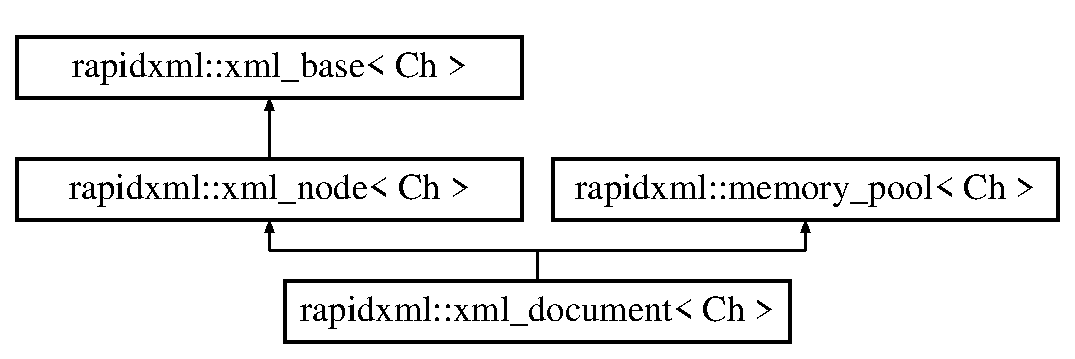
\includegraphics[height=3.000000cm]{classrapidxml_1_1xml__document}
\end{center}
\end{figure}
\subsection*{Classes}
\begin{DoxyCompactItemize}
\item 
struct \hyperlink{structrapidxml_1_1xml__document_1_1attribute__name__pred}{attribute\+\_\+name\+\_\+pred}
\item 
struct \hyperlink{structrapidxml_1_1xml__document_1_1attribute__value__pred}{attribute\+\_\+value\+\_\+pred}
\item 
struct \hyperlink{structrapidxml_1_1xml__document_1_1attribute__value__pure__pred}{attribute\+\_\+value\+\_\+pure\+\_\+pred}
\item 
struct \hyperlink{structrapidxml_1_1xml__document_1_1node__name__pred}{node\+\_\+name\+\_\+pred}
\item 
struct \hyperlink{structrapidxml_1_1xml__document_1_1text__pred}{text\+\_\+pred}
\item 
struct \hyperlink{structrapidxml_1_1xml__document_1_1text__pure__no__ws__pred}{text\+\_\+pure\+\_\+no\+\_\+ws\+\_\+pred}
\item 
struct \hyperlink{structrapidxml_1_1xml__document_1_1text__pure__with__ws__pred}{text\+\_\+pure\+\_\+with\+\_\+ws\+\_\+pred}
\item 
struct \hyperlink{structrapidxml_1_1xml__document_1_1whitespace__pred}{whitespace\+\_\+pred}
\end{DoxyCompactItemize}
\subsection*{Public Member Functions}
\begin{DoxyCompactItemize}
\item 
\hyperlink{classrapidxml_1_1xml__document_aae8841b15085ba8f32ff46587ace28f5}{xml\+\_\+document} ()
\begin{DoxyCompactList}\small\item\em Constructs empty X\+M\+L document. \end{DoxyCompactList}\item 
{\footnotesize template$<$int Flags$>$ }\\void \hyperlink{classrapidxml_1_1xml__document_ac6e73ff9ac323bf5a370c38feb03a6b1}{parse} (Ch $\ast$text)
\item 
void \hyperlink{classrapidxml_1_1xml__document_a826929ff54242532198701f19ff5f83f}{clear} ()
\item 
\hyperlink{namespacerapidxml_abb456db38f7efb746c4330eed6072a7c}{node\+\_\+type} \hyperlink{classrapidxml_1_1xml__node_a2c6a4315b98bcfa2e04fed3fa1b22c36}{type} () const 
\item 
void \hyperlink{classrapidxml_1_1xml__node_a499bbc9300c1b06821d5c08b24164c68}{type} (\hyperlink{namespacerapidxml_abb456db38f7efb746c4330eed6072a7c}{node\+\_\+type} type)
\item 
\hyperlink{classrapidxml_1_1xml__document}{xml\+\_\+document}$<$ Ch $>$ $\ast$ \hyperlink{classrapidxml_1_1xml__node_adb6ad21a4590cf13d4a6a5036e3cdbbc}{document} () const 
\item 
\hyperlink{classrapidxml_1_1xml__node}{xml\+\_\+node}$<$ Ch $>$ $\ast$ \hyperlink{classrapidxml_1_1xml__node_a2dedeb4e04bb35e06a9a7bddf6ba652d}{first\+\_\+node} (const Ch $\ast$\hyperlink{classrapidxml_1_1xml__base_a9a09739310469995db078ebd0da3ed45}{name}=0, std\+::size\+\_\+t \hyperlink{classrapidxml_1_1xml__base_a7e7f98b3d01e1eab8dc1ca69aad9af84}{name\+\_\+size}=0, bool case\+\_\+sensitive=true) const 
\item 
\hyperlink{classrapidxml_1_1xml__node}{xml\+\_\+node}$<$ Ch $>$ $\ast$ \hyperlink{classrapidxml_1_1xml__node_a2ace550c18cf10da6303773972d7157f}{last\+\_\+node} (const Ch $\ast$\hyperlink{classrapidxml_1_1xml__base_a9a09739310469995db078ebd0da3ed45}{name}=0, std\+::size\+\_\+t \hyperlink{classrapidxml_1_1xml__base_a7e7f98b3d01e1eab8dc1ca69aad9af84}{name\+\_\+size}=0, bool case\+\_\+sensitive=true) const 
\item 
\hyperlink{classrapidxml_1_1xml__node}{xml\+\_\+node}$<$ Ch $>$ $\ast$ \hyperlink{classrapidxml_1_1xml__node_a001ece4e227eebbd6ad0ec7dacf1c00b}{previous\+\_\+sibling} (const Ch $\ast$\hyperlink{classrapidxml_1_1xml__base_a9a09739310469995db078ebd0da3ed45}{name}=0, std\+::size\+\_\+t \hyperlink{classrapidxml_1_1xml__base_a7e7f98b3d01e1eab8dc1ca69aad9af84}{name\+\_\+size}=0, bool case\+\_\+sensitive=true) const 
\item 
\hyperlink{classrapidxml_1_1xml__node}{xml\+\_\+node}$<$ Ch $>$ $\ast$ \hyperlink{classrapidxml_1_1xml__node_ac59af4dd5f0ec715753e42467dff6aed}{next\+\_\+sibling} (const Ch $\ast$\hyperlink{classrapidxml_1_1xml__base_a9a09739310469995db078ebd0da3ed45}{name}=0, std\+::size\+\_\+t \hyperlink{classrapidxml_1_1xml__base_a7e7f98b3d01e1eab8dc1ca69aad9af84}{name\+\_\+size}=0, bool case\+\_\+sensitive=true) const 
\item 
\hyperlink{classrapidxml_1_1xml__attribute}{xml\+\_\+attribute}$<$ Ch $>$ $\ast$ \hyperlink{classrapidxml_1_1xml__node_ae426802be58114ffc41bf30ac6b8c37d}{first\+\_\+attribute} (const Ch $\ast$\hyperlink{classrapidxml_1_1xml__base_a9a09739310469995db078ebd0da3ed45}{name}=0, std\+::size\+\_\+t \hyperlink{classrapidxml_1_1xml__base_a7e7f98b3d01e1eab8dc1ca69aad9af84}{name\+\_\+size}=0, bool case\+\_\+sensitive=true) const 
\item 
\hyperlink{classrapidxml_1_1xml__attribute}{xml\+\_\+attribute}$<$ Ch $>$ $\ast$ \hyperlink{classrapidxml_1_1xml__node_a50c03f2db3fa51f27a73d86ec29a49d3}{last\+\_\+attribute} (const Ch $\ast$\hyperlink{classrapidxml_1_1xml__base_a9a09739310469995db078ebd0da3ed45}{name}=0, std\+::size\+\_\+t \hyperlink{classrapidxml_1_1xml__base_a7e7f98b3d01e1eab8dc1ca69aad9af84}{name\+\_\+size}=0, bool case\+\_\+sensitive=true) const 
\item 
void \hyperlink{classrapidxml_1_1xml__node_ae86e92908c3eab40bbed8216e4f3f3cb}{prepend\+\_\+node} (\hyperlink{classrapidxml_1_1xml__node}{xml\+\_\+node}$<$ Ch $>$ $\ast$child)
\item 
void \hyperlink{classrapidxml_1_1xml__node_a8696d098ecc9c4d2a646b43e91d58e31}{append\+\_\+node} (\hyperlink{classrapidxml_1_1xml__node}{xml\+\_\+node}$<$ Ch $>$ $\ast$child)
\item 
void \hyperlink{classrapidxml_1_1xml__node_a666880f42a7e486d78cc45ed51c7c46d}{insert\+\_\+node} (\hyperlink{classrapidxml_1_1xml__node}{xml\+\_\+node}$<$ Ch $>$ $\ast$where, \hyperlink{classrapidxml_1_1xml__node}{xml\+\_\+node}$<$ Ch $>$ $\ast$child)
\item 
void \hyperlink{classrapidxml_1_1xml__node_a62bf7b276cf7a651a3337f5e0a0ef6ac}{remove\+\_\+first\+\_\+node} ()
\item 
void \hyperlink{classrapidxml_1_1xml__node_a9182512e948ec451a83f116cce7c7674}{remove\+\_\+last\+\_\+node} ()
\item 
void \hyperlink{classrapidxml_1_1xml__node_a98289923eb9e8889418a9eb0207ea35c}{remove\+\_\+node} (\hyperlink{classrapidxml_1_1xml__node}{xml\+\_\+node}$<$ Ch $>$ $\ast$where)
\begin{DoxyCompactList}\small\item\em Removes specified child from the node. \end{DoxyCompactList}\item 
void \hyperlink{classrapidxml_1_1xml__node_a95735358b079ae0adcfbbac69aa1fbc3}{remove\+\_\+all\+\_\+nodes} ()
\begin{DoxyCompactList}\small\item\em Removes all child nodes (but not attributes). \end{DoxyCompactList}\item 
void \hyperlink{classrapidxml_1_1xml__node_a8b62ee76489faf8e2d1210869d547684}{prepend\+\_\+attribute} (\hyperlink{classrapidxml_1_1xml__attribute}{xml\+\_\+attribute}$<$ Ch $>$ $\ast$attribute)
\item 
void \hyperlink{classrapidxml_1_1xml__node_a33ce3386f8c42dd4db658b75cbb6e6c4}{append\+\_\+attribute} (\hyperlink{classrapidxml_1_1xml__attribute}{xml\+\_\+attribute}$<$ Ch $>$ $\ast$attribute)
\item 
void \hyperlink{classrapidxml_1_1xml__node_a9fe659cdf4a5b3bbf5e8ffc98db5a84f}{insert\+\_\+attribute} (\hyperlink{classrapidxml_1_1xml__attribute}{xml\+\_\+attribute}$<$ Ch $>$ $\ast$where, \hyperlink{classrapidxml_1_1xml__attribute}{xml\+\_\+attribute}$<$ Ch $>$ $\ast$attribute)
\item 
void \hyperlink{classrapidxml_1_1xml__node_aa95192d2a165cca16c551ed2a2a06aec}{remove\+\_\+first\+\_\+attribute} ()
\item 
void \hyperlink{classrapidxml_1_1xml__node_a1781a2cbedc9a51d609ad5b528125635}{remove\+\_\+last\+\_\+attribute} ()
\item 
void \hyperlink{classrapidxml_1_1xml__node_a6f97b1b4f46a94a4587915df3c0c6b57}{remove\+\_\+attribute} (\hyperlink{classrapidxml_1_1xml__attribute}{xml\+\_\+attribute}$<$ Ch $>$ $\ast$where)
\item 
void \hyperlink{classrapidxml_1_1xml__node_aa8d5d9484aa1eb5ff1841a073c84c1aa}{remove\+\_\+all\+\_\+attributes} ()
\begin{DoxyCompactList}\small\item\em Removes all attributes of node. \end{DoxyCompactList}\item 
Ch $\ast$ \hyperlink{classrapidxml_1_1xml__base_a9a09739310469995db078ebd0da3ed45}{name} () const 
\item 
void \hyperlink{classrapidxml_1_1xml__base_ae55060ae958c6e6465d6c8db852ec6ce}{name} (const Ch $\ast$name, std\+::size\+\_\+t size)
\item 
void \hyperlink{classrapidxml_1_1xml__base_a4611ddc82ac83a527c65606600eb2a0d}{name} (const Ch $\ast$name)
\item 
std\+::size\+\_\+t \hyperlink{classrapidxml_1_1xml__base_a7e7f98b3d01e1eab8dc1ca69aad9af84}{name\+\_\+size} () const 
\item 
Ch $\ast$ \hyperlink{classrapidxml_1_1xml__base_adcdaccff61c665f039d9344e447b7445}{value} () const 
\item 
void \hyperlink{classrapidxml_1_1xml__base_a3b183c2db7022a6d30494dd2f0ac11e9}{value} (const Ch $\ast$value, std\+::size\+\_\+t size)
\item 
void \hyperlink{classrapidxml_1_1xml__base_a81e63ec4bfd2d7ef0a6c2ed49be6e623}{value} (const Ch $\ast$value)
\item 
std\+::size\+\_\+t \hyperlink{classrapidxml_1_1xml__base_a9fcf201ed0915ac18dd43b0b5dcfaf32}{value\+\_\+size} () const 
\item 
\hyperlink{classrapidxml_1_1xml__node}{xml\+\_\+node}$<$ Ch $>$ $\ast$ \hyperlink{classrapidxml_1_1xml__base_a7f31ae930f93852830234db1ae59c4c4}{parent} () const 
\item 
\hyperlink{classrapidxml_1_1xml__node}{xml\+\_\+node}$<$ Ch $>$ $\ast$ \hyperlink{classrapidxml_1_1memory__pool_a4118581c29ee9a2f6b55ebf7dac185f8}{allocate\+\_\+node} (\hyperlink{namespacerapidxml_abb456db38f7efb746c4330eed6072a7c}{node\+\_\+type} \hyperlink{classrapidxml_1_1xml__node_a2c6a4315b98bcfa2e04fed3fa1b22c36}{type}, const Ch $\ast$\hyperlink{classrapidxml_1_1xml__base_a9a09739310469995db078ebd0da3ed45}{name}=0, const Ch $\ast$\hyperlink{classrapidxml_1_1xml__base_adcdaccff61c665f039d9344e447b7445}{value}=0, std\+::size\+\_\+t \hyperlink{classrapidxml_1_1xml__base_a7e7f98b3d01e1eab8dc1ca69aad9af84}{name\+\_\+size}=0, std\+::size\+\_\+t \hyperlink{classrapidxml_1_1xml__base_a9fcf201ed0915ac18dd43b0b5dcfaf32}{value\+\_\+size}=0)
\item 
\hyperlink{classrapidxml_1_1xml__attribute}{xml\+\_\+attribute}$<$ Ch $>$ $\ast$ \hyperlink{classrapidxml_1_1memory__pool_a3de2a66c983336e006ea3844e244ed30}{allocate\+\_\+attribute} (const Ch $\ast$\hyperlink{classrapidxml_1_1xml__base_a9a09739310469995db078ebd0da3ed45}{name}=0, const Ch $\ast$\hyperlink{classrapidxml_1_1xml__base_adcdaccff61c665f039d9344e447b7445}{value}=0, std\+::size\+\_\+t \hyperlink{classrapidxml_1_1xml__base_a7e7f98b3d01e1eab8dc1ca69aad9af84}{name\+\_\+size}=0, std\+::size\+\_\+t \hyperlink{classrapidxml_1_1xml__base_a9fcf201ed0915ac18dd43b0b5dcfaf32}{value\+\_\+size}=0)
\item 
Ch $\ast$ \hyperlink{classrapidxml_1_1memory__pool_a171941b39d55b868358da97462185f58}{allocate\+\_\+string} (const Ch $\ast$source=0, std\+::size\+\_\+t size=0)
\item 
\hyperlink{classrapidxml_1_1xml__node}{xml\+\_\+node}$<$ Ch $>$ $\ast$ \hyperlink{classrapidxml_1_1memory__pool_a0a10679fc17597d339a0dc107f8a94ac}{clone\+\_\+node} (const \hyperlink{classrapidxml_1_1xml__node}{xml\+\_\+node}$<$ Ch $>$ $\ast$source, \hyperlink{classrapidxml_1_1xml__node}{xml\+\_\+node}$<$ Ch $>$ $\ast$result=0)
\item 
void \hyperlink{classrapidxml_1_1memory__pool_a84d3d8d2cdfc00501e1dcf26d889ae03}{set\+\_\+allocator} (alloc\+\_\+func $\ast$af, free\+\_\+func $\ast$ff)
\end{DoxyCompactItemize}
\subsection*{Static Protected Member Functions}
\begin{DoxyCompactItemize}
\item 
static Ch $\ast$ \hyperlink{classrapidxml_1_1xml__base_ad96ff6b1e41dab3ff60b9bc4df769a75}{nullstr} ()
\end{DoxyCompactItemize}
\subsection*{Protected Attributes}
\begin{DoxyCompactItemize}
\item 
Ch $\ast$ \hyperlink{classrapidxml_1_1xml__base_afd9851ed43e14619db0d7075ef8e9e8a}{m\+\_\+name}
\item 
Ch $\ast$ \hyperlink{classrapidxml_1_1xml__base_a278a1ea63b0b70219b946cec47fa00ea}{m\+\_\+value}
\item 
std\+::size\+\_\+t \hyperlink{classrapidxml_1_1xml__base_a5a8c76a7274b4180213796422c4df76f}{m\+\_\+name\+\_\+size}
\item 
std\+::size\+\_\+t \hyperlink{classrapidxml_1_1xml__base_aa3a49d8ceddb8a8d7edb773a2226b89c}{m\+\_\+value\+\_\+size}
\item 
\hyperlink{classrapidxml_1_1xml__node}{xml\+\_\+node}$<$ Ch $>$ $\ast$ \hyperlink{classrapidxml_1_1xml__base_a90d5f660f078f66563fd7b2d8387ccb0}{m\+\_\+parent}
\end{DoxyCompactItemize}
\subsection*{Private Member Functions}
\begin{DoxyCompactItemize}
\item 
{\footnotesize template$<$int Flags$>$ }\\void \hyperlink{classrapidxml_1_1xml__document_aaa63a0c7b57ab8fce63d4aebe4da123d}{parse\+\_\+bom} (Ch $\ast$\&text)
\item 
{\footnotesize template$<$int Flags$>$ }\\\hyperlink{classrapidxml_1_1xml__node}{xml\+\_\+node}$<$ Ch $>$ $\ast$ \hyperlink{classrapidxml_1_1xml__document_a0151c52c82ba79ea0605c2facf39c534}{parse\+\_\+xml\+\_\+declaration} (Ch $\ast$\&text)
\item 
{\footnotesize template$<$int Flags$>$ }\\\hyperlink{classrapidxml_1_1xml__node}{xml\+\_\+node}$<$ Ch $>$ $\ast$ \hyperlink{classrapidxml_1_1xml__document_abc287ce83bcb2dc8519e300236004591}{parse\+\_\+comment} (Ch $\ast$\&text)
\item 
{\footnotesize template$<$int Flags$>$ }\\\hyperlink{classrapidxml_1_1xml__node}{xml\+\_\+node}$<$ Ch $>$ $\ast$ \hyperlink{classrapidxml_1_1xml__document_a4c613f3a928f763b4c788422edda5860}{parse\+\_\+doctype} (Ch $\ast$\&text)
\item 
{\footnotesize template$<$int Flags$>$ }\\\hyperlink{classrapidxml_1_1xml__node}{xml\+\_\+node}$<$ Ch $>$ $\ast$ \hyperlink{classrapidxml_1_1xml__document_a09e12a4233a07387d4b5a5ad239388aa}{parse\+\_\+pi} (Ch $\ast$\&text)
\item 
{\footnotesize template$<$int Flags$>$ }\\Ch \hyperlink{classrapidxml_1_1xml__document_aec6cedf45179b6378c670bc3ea509e61}{parse\+\_\+and\+\_\+append\+\_\+data} (\hyperlink{classrapidxml_1_1xml__node}{xml\+\_\+node}$<$ Ch $>$ $\ast$node, Ch $\ast$\&text, Ch $\ast$contents\+\_\+start)
\item 
{\footnotesize template$<$int Flags$>$ }\\\hyperlink{classrapidxml_1_1xml__node}{xml\+\_\+node}$<$ Ch $>$ $\ast$ \hyperlink{classrapidxml_1_1xml__document_ab94daeb25e8a1609e31210a45b2afa6c}{parse\+\_\+cdata} (Ch $\ast$\&text)
\item 
{\footnotesize template$<$int Flags$>$ }\\\hyperlink{classrapidxml_1_1xml__node}{xml\+\_\+node}$<$ Ch $>$ $\ast$ \hyperlink{classrapidxml_1_1xml__document_aea385acd096ab200d63a777d53435ada}{parse\+\_\+element} (Ch $\ast$\&text)
\item 
{\footnotesize template$<$int Flags$>$ }\\\hyperlink{classrapidxml_1_1xml__node}{xml\+\_\+node}$<$ Ch $>$ $\ast$ \hyperlink{classrapidxml_1_1xml__document_a5e94cbc9b02e864cb80961ddb8cc63a7}{parse\+\_\+node} (Ch $\ast$\&text)
\item 
{\footnotesize template$<$int Flags$>$ }\\void \hyperlink{classrapidxml_1_1xml__document_aae0a4c2e1972ab9a9e0ce91cf1166ac9}{parse\+\_\+node\+\_\+contents} (Ch $\ast$\&text, \hyperlink{classrapidxml_1_1xml__node}{xml\+\_\+node}$<$ Ch $>$ $\ast$node)
\item 
{\footnotesize template$<$int Flags$>$ }\\void \hyperlink{classrapidxml_1_1xml__document_ac0b3cd07b3d5cbaa83762a196c681519}{parse\+\_\+node\+\_\+attributes} (Ch $\ast$\&text, \hyperlink{classrapidxml_1_1xml__node}{xml\+\_\+node}$<$ Ch $>$ $\ast$node)
\end{DoxyCompactItemize}
\subsection*{Static Private Member Functions}
\begin{DoxyCompactItemize}
\item 
{\footnotesize template$<$int Flags$>$ }\\static void \hyperlink{classrapidxml_1_1xml__document_ae33040bcfa8e5a29dc6f6f130984a981}{insert\+\_\+coded\+\_\+character} (Ch $\ast$\&text, unsigned long code)
\item 
{\footnotesize template$<$class Stop\+Pred , int Flags$>$ }\\static void \hyperlink{classrapidxml_1_1xml__document_a27aca5bdcb3bfa899f61b17d7f1d3a0d}{skip} (Ch $\ast$\&text)
\item 
{\footnotesize template$<$class Stop\+Pred , class Stop\+Pred\+Pure , int Flags$>$ }\\static Ch $\ast$ \hyperlink{classrapidxml_1_1xml__document_af86781975cdfff2105fa8c0b49ab4507}{skip\+\_\+and\+\_\+expand\+\_\+character\+\_\+refs} (Ch $\ast$\&text)
\end{DoxyCompactItemize}


\subsection{Detailed Description}
\subsubsection*{template$<$class Ch = char$>$class rapidxml\+::xml\+\_\+document$<$ Ch $>$}

This class represents root of the D\+O\+M hierarchy. It is also an \hyperlink{classrapidxml_1_1xml__node}{xml\+\_\+node} and a \hyperlink{classrapidxml_1_1memory__pool}{memory\+\_\+pool} through public inheritance. Use \hyperlink{classrapidxml_1_1xml__document_ac6e73ff9ac323bf5a370c38feb03a6b1}{parse()} function to build a D\+O\+M tree from a zero-\/terminated X\+M\+L text string. \hyperlink{classrapidxml_1_1xml__document_ac6e73ff9ac323bf5a370c38feb03a6b1}{parse()} function allocates memory for nodes and attributes by using functions of \hyperlink{classrapidxml_1_1xml__document}{xml\+\_\+document}, which are inherited from \hyperlink{classrapidxml_1_1memory__pool}{memory\+\_\+pool}. To access root node of the document, use the document itself, as if it was an \hyperlink{classrapidxml_1_1xml__node}{xml\+\_\+node}. 
\begin{DoxyParams}{Parameters}
{\em Ch} & Character type to use. \\
\hline
\end{DoxyParams}


\subsection{Constructor \& Destructor Documentation}
\hypertarget{classrapidxml_1_1xml__document_aae8841b15085ba8f32ff46587ace28f5}{}\index{rapidxml\+::xml\+\_\+document@{rapidxml\+::xml\+\_\+document}!xml\+\_\+document@{xml\+\_\+document}}
\index{xml\+\_\+document@{xml\+\_\+document}!rapidxml\+::xml\+\_\+document@{rapidxml\+::xml\+\_\+document}}
\subsubsection[{xml\+\_\+document}]{\setlength{\rightskip}{0pt plus 5cm}template$<$class Ch  = char$>$ {\bf rapidxml\+::xml\+\_\+document}$<$ Ch $>$\+::{\bf xml\+\_\+document} (
\begin{DoxyParamCaption}
{}
\end{DoxyParamCaption}
)\hspace{0.3cm}{\ttfamily [inline]}}\label{classrapidxml_1_1xml__document_aae8841b15085ba8f32ff46587ace28f5}


Constructs empty X\+M\+L document. 



\subsection{Member Function Documentation}
\hypertarget{classrapidxml_1_1memory__pool_a3de2a66c983336e006ea3844e244ed30}{}\index{rapidxml\+::xml\+\_\+document@{rapidxml\+::xml\+\_\+document}!allocate\+\_\+attribute@{allocate\+\_\+attribute}}
\index{allocate\+\_\+attribute@{allocate\+\_\+attribute}!rapidxml\+::xml\+\_\+document@{rapidxml\+::xml\+\_\+document}}
\subsubsection[{allocate\+\_\+attribute}]{\setlength{\rightskip}{0pt plus 5cm}template$<$class Ch  = char$>$ {\bf xml\+\_\+attribute}$<$Ch$>$$\ast$ {\bf rapidxml\+::memory\+\_\+pool}$<$ Ch $>$\+::allocate\+\_\+attribute (
\begin{DoxyParamCaption}
\item[{const Ch $\ast$}]{name = {\ttfamily 0}, }
\item[{const Ch $\ast$}]{value = {\ttfamily 0}, }
\item[{std\+::size\+\_\+t}]{name\+\_\+size = {\ttfamily 0}, }
\item[{std\+::size\+\_\+t}]{value\+\_\+size = {\ttfamily 0}}
\end{DoxyParamCaption}
)\hspace{0.3cm}{\ttfamily [inline]}, {\ttfamily [inherited]}}\label{classrapidxml_1_1memory__pool_a3de2a66c983336e006ea3844e244ed30}
Allocates a new attribute from the pool, and optionally assigns name and value to it. If the allocation request cannot be accomodated, this function will throw {\ttfamily std\+::bad\+\_\+alloc}. If exceptions are disabled by defining R\+A\+P\+I\+D\+X\+M\+L\+\_\+\+N\+O\+\_\+\+E\+X\+C\+E\+P\+T\+I\+O\+N\+S, this function will call rapidxml\+::parse\+\_\+error\+\_\+handler() function. 
\begin{DoxyParams}{Parameters}
{\em name} & Name to assign to the attribute, or 0 to assign no name. \\
\hline
{\em value} & Value to assign to the attribute, or 0 to assign no value. \\
\hline
{\em name\+\_\+size} & Size of name to assign, or 0 to automatically calculate size from name string. \\
\hline
{\em value\+\_\+size} & Size of value to assign, or 0 to automatically calculate size from value string. \\
\hline
\end{DoxyParams}
\begin{DoxyReturn}{Returns}
Pointer to allocated attribute. This pointer will never be N\+U\+L\+L. 
\end{DoxyReturn}
\hypertarget{classrapidxml_1_1memory__pool_a4118581c29ee9a2f6b55ebf7dac185f8}{}\index{rapidxml\+::xml\+\_\+document@{rapidxml\+::xml\+\_\+document}!allocate\+\_\+node@{allocate\+\_\+node}}
\index{allocate\+\_\+node@{allocate\+\_\+node}!rapidxml\+::xml\+\_\+document@{rapidxml\+::xml\+\_\+document}}
\subsubsection[{allocate\+\_\+node}]{\setlength{\rightskip}{0pt plus 5cm}template$<$class Ch  = char$>$ {\bf xml\+\_\+node}$<$Ch$>$$\ast$ {\bf rapidxml\+::memory\+\_\+pool}$<$ Ch $>$\+::allocate\+\_\+node (
\begin{DoxyParamCaption}
\item[{{\bf node\+\_\+type}}]{type, }
\item[{const Ch $\ast$}]{name = {\ttfamily 0}, }
\item[{const Ch $\ast$}]{value = {\ttfamily 0}, }
\item[{std\+::size\+\_\+t}]{name\+\_\+size = {\ttfamily 0}, }
\item[{std\+::size\+\_\+t}]{value\+\_\+size = {\ttfamily 0}}
\end{DoxyParamCaption}
)\hspace{0.3cm}{\ttfamily [inline]}, {\ttfamily [inherited]}}\label{classrapidxml_1_1memory__pool_a4118581c29ee9a2f6b55ebf7dac185f8}
Allocates a new node from the pool, and optionally assigns name and value to it. If the allocation request cannot be accomodated, this function will throw {\ttfamily std\+::bad\+\_\+alloc}. If exceptions are disabled by defining R\+A\+P\+I\+D\+X\+M\+L\+\_\+\+N\+O\+\_\+\+E\+X\+C\+E\+P\+T\+I\+O\+N\+S, this function will call rapidxml\+::parse\+\_\+error\+\_\+handler() function. 
\begin{DoxyParams}{Parameters}
{\em type} & Type of node to create. \\
\hline
{\em name} & Name to assign to the node, or 0 to assign no name. \\
\hline
{\em value} & Value to assign to the node, or 0 to assign no value. \\
\hline
{\em name\+\_\+size} & Size of name to assign, or 0 to automatically calculate size from name string. \\
\hline
{\em value\+\_\+size} & Size of value to assign, or 0 to automatically calculate size from value string. \\
\hline
\end{DoxyParams}
\begin{DoxyReturn}{Returns}
Pointer to allocated node. This pointer will never be N\+U\+L\+L. 
\end{DoxyReturn}
\hypertarget{classrapidxml_1_1memory__pool_a171941b39d55b868358da97462185f58}{}\index{rapidxml\+::xml\+\_\+document@{rapidxml\+::xml\+\_\+document}!allocate\+\_\+string@{allocate\+\_\+string}}
\index{allocate\+\_\+string@{allocate\+\_\+string}!rapidxml\+::xml\+\_\+document@{rapidxml\+::xml\+\_\+document}}
\subsubsection[{allocate\+\_\+string}]{\setlength{\rightskip}{0pt plus 5cm}template$<$class Ch  = char$>$ Ch$\ast$ {\bf rapidxml\+::memory\+\_\+pool}$<$ Ch $>$\+::allocate\+\_\+string (
\begin{DoxyParamCaption}
\item[{const Ch $\ast$}]{source = {\ttfamily 0}, }
\item[{std\+::size\+\_\+t}]{size = {\ttfamily 0}}
\end{DoxyParamCaption}
)\hspace{0.3cm}{\ttfamily [inline]}, {\ttfamily [inherited]}}\label{classrapidxml_1_1memory__pool_a171941b39d55b868358da97462185f58}
Allocates a char array of given size from the pool, and optionally copies a given string to it. If the allocation request cannot be accomodated, this function will throw {\ttfamily std\+::bad\+\_\+alloc}. If exceptions are disabled by defining R\+A\+P\+I\+D\+X\+M\+L\+\_\+\+N\+O\+\_\+\+E\+X\+C\+E\+P\+T\+I\+O\+N\+S, this function will call rapidxml\+::parse\+\_\+error\+\_\+handler() function. 
\begin{DoxyParams}{Parameters}
{\em source} & String to initialize the allocated memory with, or 0 to not initialize it. \\
\hline
{\em size} & Number of characters to allocate, or zero to calculate it automatically from source string length; if size is 0, source string must be specified and null terminated. \\
\hline
\end{DoxyParams}
\begin{DoxyReturn}{Returns}
Pointer to allocated char array. This pointer will never be N\+U\+L\+L. 
\end{DoxyReturn}
\hypertarget{classrapidxml_1_1xml__node_a33ce3386f8c42dd4db658b75cbb6e6c4}{}\index{rapidxml\+::xml\+\_\+document@{rapidxml\+::xml\+\_\+document}!append\+\_\+attribute@{append\+\_\+attribute}}
\index{append\+\_\+attribute@{append\+\_\+attribute}!rapidxml\+::xml\+\_\+document@{rapidxml\+::xml\+\_\+document}}
\subsubsection[{append\+\_\+attribute}]{\setlength{\rightskip}{0pt plus 5cm}template$<$class Ch = char$>$ void {\bf rapidxml\+::xml\+\_\+node}$<$ Ch $>$\+::append\+\_\+attribute (
\begin{DoxyParamCaption}
\item[{{\bf xml\+\_\+attribute}$<$ Ch $>$ $\ast$}]{attribute}
\end{DoxyParamCaption}
)\hspace{0.3cm}{\ttfamily [inline]}, {\ttfamily [inherited]}}\label{classrapidxml_1_1xml__node_a33ce3386f8c42dd4db658b75cbb6e6c4}
Appends a new attribute to the node. 
\begin{DoxyParams}{Parameters}
{\em attribute} & Attribute to append. \\
\hline
\end{DoxyParams}
\hypertarget{classrapidxml_1_1xml__node_a8696d098ecc9c4d2a646b43e91d58e31}{}\index{rapidxml\+::xml\+\_\+document@{rapidxml\+::xml\+\_\+document}!append\+\_\+node@{append\+\_\+node}}
\index{append\+\_\+node@{append\+\_\+node}!rapidxml\+::xml\+\_\+document@{rapidxml\+::xml\+\_\+document}}
\subsubsection[{append\+\_\+node}]{\setlength{\rightskip}{0pt plus 5cm}template$<$class Ch = char$>$ void {\bf rapidxml\+::xml\+\_\+node}$<$ Ch $>$\+::append\+\_\+node (
\begin{DoxyParamCaption}
\item[{{\bf xml\+\_\+node}$<$ Ch $>$ $\ast$}]{child}
\end{DoxyParamCaption}
)\hspace{0.3cm}{\ttfamily [inline]}, {\ttfamily [inherited]}}\label{classrapidxml_1_1xml__node_a8696d098ecc9c4d2a646b43e91d58e31}
Appends a new child node. The appended child becomes the last child. 
\begin{DoxyParams}{Parameters}
{\em child} & Node to append. \\
\hline
\end{DoxyParams}
\hypertarget{classrapidxml_1_1xml__document_a826929ff54242532198701f19ff5f83f}{}\index{rapidxml\+::xml\+\_\+document@{rapidxml\+::xml\+\_\+document}!clear@{clear}}
\index{clear@{clear}!rapidxml\+::xml\+\_\+document@{rapidxml\+::xml\+\_\+document}}
\subsubsection[{clear}]{\setlength{\rightskip}{0pt plus 5cm}template$<$class Ch  = char$>$ void {\bf rapidxml\+::xml\+\_\+document}$<$ Ch $>$\+::clear (
\begin{DoxyParamCaption}
{}
\end{DoxyParamCaption}
)\hspace{0.3cm}{\ttfamily [inline]}}\label{classrapidxml_1_1xml__document_a826929ff54242532198701f19ff5f83f}
Clears the document by deleting all nodes and clearing the memory pool. All nodes owned by document pool are destroyed. \hypertarget{classrapidxml_1_1memory__pool_a0a10679fc17597d339a0dc107f8a94ac}{}\index{rapidxml\+::xml\+\_\+document@{rapidxml\+::xml\+\_\+document}!clone\+\_\+node@{clone\+\_\+node}}
\index{clone\+\_\+node@{clone\+\_\+node}!rapidxml\+::xml\+\_\+document@{rapidxml\+::xml\+\_\+document}}
\subsubsection[{clone\+\_\+node}]{\setlength{\rightskip}{0pt plus 5cm}template$<$class Ch  = char$>$ {\bf xml\+\_\+node}$<$Ch$>$$\ast$ {\bf rapidxml\+::memory\+\_\+pool}$<$ Ch $>$\+::clone\+\_\+node (
\begin{DoxyParamCaption}
\item[{const {\bf xml\+\_\+node}$<$ Ch $>$ $\ast$}]{source, }
\item[{{\bf xml\+\_\+node}$<$ Ch $>$ $\ast$}]{result = {\ttfamily 0}}
\end{DoxyParamCaption}
)\hspace{0.3cm}{\ttfamily [inline]}, {\ttfamily [inherited]}}\label{classrapidxml_1_1memory__pool_a0a10679fc17597d339a0dc107f8a94ac}
Clones an \hyperlink{classrapidxml_1_1xml__node}{xml\+\_\+node} and its hierarchy of child nodes and attributes. Nodes and attributes are allocated from this memory pool. Names and values are not cloned, they are shared between the clone and the source. Result node can be optionally specified as a second parameter, in which case its contents will be replaced with cloned source node. This is useful when you want to clone entire document. 
\begin{DoxyParams}{Parameters}
{\em source} & Node to clone. \\
\hline
{\em result} & Node to put results in, or 0 to automatically allocate result node \\
\hline
\end{DoxyParams}
\begin{DoxyReturn}{Returns}
Pointer to cloned node. This pointer will never be N\+U\+L\+L. 
\end{DoxyReturn}
\hypertarget{classrapidxml_1_1xml__node_adb6ad21a4590cf13d4a6a5036e3cdbbc}{}\index{rapidxml\+::xml\+\_\+document@{rapidxml\+::xml\+\_\+document}!document@{document}}
\index{document@{document}!rapidxml\+::xml\+\_\+document@{rapidxml\+::xml\+\_\+document}}
\subsubsection[{document}]{\setlength{\rightskip}{0pt plus 5cm}template$<$class Ch = char$>$ {\bf xml\+\_\+document}$<$Ch$>$$\ast$ {\bf rapidxml\+::xml\+\_\+node}$<$ Ch $>$\+::document (
\begin{DoxyParamCaption}
{}
\end{DoxyParamCaption}
) const\hspace{0.3cm}{\ttfamily [inline]}, {\ttfamily [inherited]}}\label{classrapidxml_1_1xml__node_adb6ad21a4590cf13d4a6a5036e3cdbbc}
Gets document of which node is a child. \begin{DoxyReturn}{Returns}
Pointer to document that contains this node, or 0 if there is no parent document. 
\end{DoxyReturn}
\hypertarget{classrapidxml_1_1xml__node_ae426802be58114ffc41bf30ac6b8c37d}{}\index{rapidxml\+::xml\+\_\+document@{rapidxml\+::xml\+\_\+document}!first\+\_\+attribute@{first\+\_\+attribute}}
\index{first\+\_\+attribute@{first\+\_\+attribute}!rapidxml\+::xml\+\_\+document@{rapidxml\+::xml\+\_\+document}}
\subsubsection[{first\+\_\+attribute}]{\setlength{\rightskip}{0pt plus 5cm}template$<$class Ch = char$>$ {\bf xml\+\_\+attribute}$<$Ch$>$$\ast$ {\bf rapidxml\+::xml\+\_\+node}$<$ Ch $>$\+::first\+\_\+attribute (
\begin{DoxyParamCaption}
\item[{const Ch $\ast$}]{name = {\ttfamily 0}, }
\item[{std\+::size\+\_\+t}]{name\+\_\+size = {\ttfamily 0}, }
\item[{bool}]{case\+\_\+sensitive = {\ttfamily true}}
\end{DoxyParamCaption}
) const\hspace{0.3cm}{\ttfamily [inline]}, {\ttfamily [inherited]}}\label{classrapidxml_1_1xml__node_ae426802be58114ffc41bf30ac6b8c37d}
Gets first attribute of node, optionally matching attribute name. 
\begin{DoxyParams}{Parameters}
{\em name} & Name of attribute to find, or 0 to return first attribute regardless of its name; this string doesn\textquotesingle{}t have to be zero-\/terminated if name\+\_\+size is non-\/zero \\
\hline
{\em name\+\_\+size} & Size of name, in characters, or 0 to have size calculated automatically from string \\
\hline
{\em case\+\_\+sensitive} & Should name comparison be case-\/sensitive; non case-\/sensitive comparison works properly only for A\+S\+C\+I\+I characters \\
\hline
\end{DoxyParams}
\begin{DoxyReturn}{Returns}
Pointer to found attribute, or 0 if not found. 
\end{DoxyReturn}
\hypertarget{classrapidxml_1_1xml__node_a2dedeb4e04bb35e06a9a7bddf6ba652d}{}\index{rapidxml\+::xml\+\_\+document@{rapidxml\+::xml\+\_\+document}!first\+\_\+node@{first\+\_\+node}}
\index{first\+\_\+node@{first\+\_\+node}!rapidxml\+::xml\+\_\+document@{rapidxml\+::xml\+\_\+document}}
\subsubsection[{first\+\_\+node}]{\setlength{\rightskip}{0pt plus 5cm}template$<$class Ch = char$>$ {\bf xml\+\_\+node}$<$Ch$>$$\ast$ {\bf rapidxml\+::xml\+\_\+node}$<$ Ch $>$\+::first\+\_\+node (
\begin{DoxyParamCaption}
\item[{const Ch $\ast$}]{name = {\ttfamily 0}, }
\item[{std\+::size\+\_\+t}]{name\+\_\+size = {\ttfamily 0}, }
\item[{bool}]{case\+\_\+sensitive = {\ttfamily true}}
\end{DoxyParamCaption}
) const\hspace{0.3cm}{\ttfamily [inline]}, {\ttfamily [inherited]}}\label{classrapidxml_1_1xml__node_a2dedeb4e04bb35e06a9a7bddf6ba652d}
Gets first child node, optionally matching node name. 
\begin{DoxyParams}{Parameters}
{\em name} & Name of child to find, or 0 to return first child regardless of its name; this string doesn\textquotesingle{}t have to be zero-\/terminated if name\+\_\+size is non-\/zero \\
\hline
{\em name\+\_\+size} & Size of name, in characters, or 0 to have size calculated automatically from string \\
\hline
{\em case\+\_\+sensitive} & Should name comparison be case-\/sensitive; non case-\/sensitive comparison works properly only for A\+S\+C\+I\+I characters \\
\hline
\end{DoxyParams}
\begin{DoxyReturn}{Returns}
Pointer to found child, or 0 if not found. 
\end{DoxyReturn}
\hypertarget{classrapidxml_1_1xml__node_a9fe659cdf4a5b3bbf5e8ffc98db5a84f}{}\index{rapidxml\+::xml\+\_\+document@{rapidxml\+::xml\+\_\+document}!insert\+\_\+attribute@{insert\+\_\+attribute}}
\index{insert\+\_\+attribute@{insert\+\_\+attribute}!rapidxml\+::xml\+\_\+document@{rapidxml\+::xml\+\_\+document}}
\subsubsection[{insert\+\_\+attribute}]{\setlength{\rightskip}{0pt plus 5cm}template$<$class Ch = char$>$ void {\bf rapidxml\+::xml\+\_\+node}$<$ Ch $>$\+::insert\+\_\+attribute (
\begin{DoxyParamCaption}
\item[{{\bf xml\+\_\+attribute}$<$ Ch $>$ $\ast$}]{where, }
\item[{{\bf xml\+\_\+attribute}$<$ Ch $>$ $\ast$}]{attribute}
\end{DoxyParamCaption}
)\hspace{0.3cm}{\ttfamily [inline]}, {\ttfamily [inherited]}}\label{classrapidxml_1_1xml__node_a9fe659cdf4a5b3bbf5e8ffc98db5a84f}
Inserts a new attribute at specified place inside the node. All attributes after and including the specified attribute are moved one position back. 
\begin{DoxyParams}{Parameters}
{\em where} & Place where to insert the attribute, or 0 to insert at the back. \\
\hline
{\em attribute} & Attribute to insert. \\
\hline
\end{DoxyParams}
\hypertarget{classrapidxml_1_1xml__document_ae33040bcfa8e5a29dc6f6f130984a981}{}\index{rapidxml\+::xml\+\_\+document@{rapidxml\+::xml\+\_\+document}!insert\+\_\+coded\+\_\+character@{insert\+\_\+coded\+\_\+character}}
\index{insert\+\_\+coded\+\_\+character@{insert\+\_\+coded\+\_\+character}!rapidxml\+::xml\+\_\+document@{rapidxml\+::xml\+\_\+document}}
\subsubsection[{insert\+\_\+coded\+\_\+character}]{\setlength{\rightskip}{0pt plus 5cm}template$<$class Ch  = char$>$ template$<$int Flags$>$ static void {\bf rapidxml\+::xml\+\_\+document}$<$ Ch $>$\+::insert\+\_\+coded\+\_\+character (
\begin{DoxyParamCaption}
\item[{Ch $\ast$\&}]{text, }
\item[{unsigned long}]{code}
\end{DoxyParamCaption}
)\hspace{0.3cm}{\ttfamily [inline]}, {\ttfamily [static]}, {\ttfamily [private]}}\label{classrapidxml_1_1xml__document_ae33040bcfa8e5a29dc6f6f130984a981}
\hypertarget{classrapidxml_1_1xml__node_a666880f42a7e486d78cc45ed51c7c46d}{}\index{rapidxml\+::xml\+\_\+document@{rapidxml\+::xml\+\_\+document}!insert\+\_\+node@{insert\+\_\+node}}
\index{insert\+\_\+node@{insert\+\_\+node}!rapidxml\+::xml\+\_\+document@{rapidxml\+::xml\+\_\+document}}
\subsubsection[{insert\+\_\+node}]{\setlength{\rightskip}{0pt plus 5cm}template$<$class Ch = char$>$ void {\bf rapidxml\+::xml\+\_\+node}$<$ Ch $>$\+::insert\+\_\+node (
\begin{DoxyParamCaption}
\item[{{\bf xml\+\_\+node}$<$ Ch $>$ $\ast$}]{where, }
\item[{{\bf xml\+\_\+node}$<$ Ch $>$ $\ast$}]{child}
\end{DoxyParamCaption}
)\hspace{0.3cm}{\ttfamily [inline]}, {\ttfamily [inherited]}}\label{classrapidxml_1_1xml__node_a666880f42a7e486d78cc45ed51c7c46d}
Inserts a new child node at specified place inside the node. All children after and including the specified node are moved one position back. 
\begin{DoxyParams}{Parameters}
{\em where} & Place where to insert the child, or 0 to insert at the back. \\
\hline
{\em child} & Node to insert. \\
\hline
\end{DoxyParams}
\hypertarget{classrapidxml_1_1xml__node_a50c03f2db3fa51f27a73d86ec29a49d3}{}\index{rapidxml\+::xml\+\_\+document@{rapidxml\+::xml\+\_\+document}!last\+\_\+attribute@{last\+\_\+attribute}}
\index{last\+\_\+attribute@{last\+\_\+attribute}!rapidxml\+::xml\+\_\+document@{rapidxml\+::xml\+\_\+document}}
\subsubsection[{last\+\_\+attribute}]{\setlength{\rightskip}{0pt plus 5cm}template$<$class Ch = char$>$ {\bf xml\+\_\+attribute}$<$Ch$>$$\ast$ {\bf rapidxml\+::xml\+\_\+node}$<$ Ch $>$\+::last\+\_\+attribute (
\begin{DoxyParamCaption}
\item[{const Ch $\ast$}]{name = {\ttfamily 0}, }
\item[{std\+::size\+\_\+t}]{name\+\_\+size = {\ttfamily 0}, }
\item[{bool}]{case\+\_\+sensitive = {\ttfamily true}}
\end{DoxyParamCaption}
) const\hspace{0.3cm}{\ttfamily [inline]}, {\ttfamily [inherited]}}\label{classrapidxml_1_1xml__node_a50c03f2db3fa51f27a73d86ec29a49d3}
Gets last attribute of node, optionally matching attribute name. 
\begin{DoxyParams}{Parameters}
{\em name} & Name of attribute to find, or 0 to return last attribute regardless of its name; this string doesn\textquotesingle{}t have to be zero-\/terminated if name\+\_\+size is non-\/zero \\
\hline
{\em name\+\_\+size} & Size of name, in characters, or 0 to have size calculated automatically from string \\
\hline
{\em case\+\_\+sensitive} & Should name comparison be case-\/sensitive; non case-\/sensitive comparison works properly only for A\+S\+C\+I\+I characters \\
\hline
\end{DoxyParams}
\begin{DoxyReturn}{Returns}
Pointer to found attribute, or 0 if not found. 
\end{DoxyReturn}
\hypertarget{classrapidxml_1_1xml__node_a2ace550c18cf10da6303773972d7157f}{}\index{rapidxml\+::xml\+\_\+document@{rapidxml\+::xml\+\_\+document}!last\+\_\+node@{last\+\_\+node}}
\index{last\+\_\+node@{last\+\_\+node}!rapidxml\+::xml\+\_\+document@{rapidxml\+::xml\+\_\+document}}
\subsubsection[{last\+\_\+node}]{\setlength{\rightskip}{0pt plus 5cm}template$<$class Ch = char$>$ {\bf xml\+\_\+node}$<$Ch$>$$\ast$ {\bf rapidxml\+::xml\+\_\+node}$<$ Ch $>$\+::last\+\_\+node (
\begin{DoxyParamCaption}
\item[{const Ch $\ast$}]{name = {\ttfamily 0}, }
\item[{std\+::size\+\_\+t}]{name\+\_\+size = {\ttfamily 0}, }
\item[{bool}]{case\+\_\+sensitive = {\ttfamily true}}
\end{DoxyParamCaption}
) const\hspace{0.3cm}{\ttfamily [inline]}, {\ttfamily [inherited]}}\label{classrapidxml_1_1xml__node_a2ace550c18cf10da6303773972d7157f}
Gets last child node, optionally matching node name. Behaviour is undefined if node has no children. Use \hyperlink{classrapidxml_1_1xml__node_a2dedeb4e04bb35e06a9a7bddf6ba652d}{first\+\_\+node()} to test if node has children. 
\begin{DoxyParams}{Parameters}
{\em name} & Name of child to find, or 0 to return last child regardless of its name; this string doesn\textquotesingle{}t have to be zero-\/terminated if name\+\_\+size is non-\/zero \\
\hline
{\em name\+\_\+size} & Size of name, in characters, or 0 to have size calculated automatically from string \\
\hline
{\em case\+\_\+sensitive} & Should name comparison be case-\/sensitive; non case-\/sensitive comparison works properly only for A\+S\+C\+I\+I characters \\
\hline
\end{DoxyParams}
\begin{DoxyReturn}{Returns}
Pointer to found child, or 0 if not found. 
\end{DoxyReturn}
\hypertarget{classrapidxml_1_1xml__base_a9a09739310469995db078ebd0da3ed45}{}\index{rapidxml\+::xml\+\_\+document@{rapidxml\+::xml\+\_\+document}!name@{name}}
\index{name@{name}!rapidxml\+::xml\+\_\+document@{rapidxml\+::xml\+\_\+document}}
\subsubsection[{name}]{\setlength{\rightskip}{0pt plus 5cm}template$<$class Ch  = char$>$ Ch$\ast$ {\bf rapidxml\+::xml\+\_\+base}$<$ Ch $>$\+::name (
\begin{DoxyParamCaption}
{}
\end{DoxyParamCaption}
) const\hspace{0.3cm}{\ttfamily [inline]}, {\ttfamily [inherited]}}\label{classrapidxml_1_1xml__base_a9a09739310469995db078ebd0da3ed45}
Gets name of the node. Interpretation of name depends on type of node. Note that name will not be zero-\/terminated if \hyperlink{namespacerapidxml_af3fc88ba6bee33482a2db81b1da36ea1}{rapidxml\+::parse\+\_\+no\+\_\+string\+\_\+terminators} option was selected during parse. ~\newline
~\newline
 Use \hyperlink{classrapidxml_1_1xml__base_a7e7f98b3d01e1eab8dc1ca69aad9af84}{name\+\_\+size()} function to determine length of the name. \begin{DoxyReturn}{Returns}
Name of node, or empty string if node has no name. 
\end{DoxyReturn}
\hypertarget{classrapidxml_1_1xml__base_ae55060ae958c6e6465d6c8db852ec6ce}{}\index{rapidxml\+::xml\+\_\+document@{rapidxml\+::xml\+\_\+document}!name@{name}}
\index{name@{name}!rapidxml\+::xml\+\_\+document@{rapidxml\+::xml\+\_\+document}}
\subsubsection[{name}]{\setlength{\rightskip}{0pt plus 5cm}template$<$class Ch  = char$>$ void {\bf rapidxml\+::xml\+\_\+base}$<$ Ch $>$\+::name (
\begin{DoxyParamCaption}
\item[{const Ch $\ast$}]{name, }
\item[{std\+::size\+\_\+t}]{size}
\end{DoxyParamCaption}
)\hspace{0.3cm}{\ttfamily [inline]}, {\ttfamily [inherited]}}\label{classrapidxml_1_1xml__base_ae55060ae958c6e6465d6c8db852ec6ce}
Sets name of node to a non zero-\/terminated string. See ownership\+\_\+of\+\_\+strings. ~\newline
~\newline
 Note that node does not own its name or value, it only stores a pointer to it. It will not delete or otherwise free the pointer on destruction. It is reponsibility of the user to properly manage lifetime of the string. The easiest way to achieve it is to use \hyperlink{classrapidxml_1_1memory__pool}{memory\+\_\+pool} of the document to allocate the string -\/ on destruction of the document the string will be automatically freed. ~\newline
~\newline
 Size of name must be specified separately, because name does not have to be zero terminated. Use \hyperlink{classrapidxml_1_1xml__base_a4611ddc82ac83a527c65606600eb2a0d}{name(const Ch $\ast$)} function to have the length automatically calculated (string must be zero terminated). 
\begin{DoxyParams}{Parameters}
{\em name} & Name of node to set. Does not have to be zero terminated. \\
\hline
{\em size} & Size of name, in characters. This does not include zero terminator, if one is present. \\
\hline
\end{DoxyParams}
\hypertarget{classrapidxml_1_1xml__base_a4611ddc82ac83a527c65606600eb2a0d}{}\index{rapidxml\+::xml\+\_\+document@{rapidxml\+::xml\+\_\+document}!name@{name}}
\index{name@{name}!rapidxml\+::xml\+\_\+document@{rapidxml\+::xml\+\_\+document}}
\subsubsection[{name}]{\setlength{\rightskip}{0pt plus 5cm}template$<$class Ch  = char$>$ void {\bf rapidxml\+::xml\+\_\+base}$<$ Ch $>$\+::name (
\begin{DoxyParamCaption}
\item[{const Ch $\ast$}]{name}
\end{DoxyParamCaption}
)\hspace{0.3cm}{\ttfamily [inline]}, {\ttfamily [inherited]}}\label{classrapidxml_1_1xml__base_a4611ddc82ac83a527c65606600eb2a0d}
Sets name of node to a zero-\/terminated string. See also ownership\+\_\+of\+\_\+strings and \hyperlink{classrapidxml_1_1xml__base_ae55060ae958c6e6465d6c8db852ec6ce}{xml\+\_\+node\+::name(const Ch $\ast$, std\+::size\+\_\+t)}. 
\begin{DoxyParams}{Parameters}
{\em name} & Name of node to set. Must be zero terminated. \\
\hline
\end{DoxyParams}
\hypertarget{classrapidxml_1_1xml__base_a7e7f98b3d01e1eab8dc1ca69aad9af84}{}\index{rapidxml\+::xml\+\_\+document@{rapidxml\+::xml\+\_\+document}!name\+\_\+size@{name\+\_\+size}}
\index{name\+\_\+size@{name\+\_\+size}!rapidxml\+::xml\+\_\+document@{rapidxml\+::xml\+\_\+document}}
\subsubsection[{name\+\_\+size}]{\setlength{\rightskip}{0pt plus 5cm}template$<$class Ch  = char$>$ std\+::size\+\_\+t {\bf rapidxml\+::xml\+\_\+base}$<$ Ch $>$\+::name\+\_\+size (
\begin{DoxyParamCaption}
{}
\end{DoxyParamCaption}
) const\hspace{0.3cm}{\ttfamily [inline]}, {\ttfamily [inherited]}}\label{classrapidxml_1_1xml__base_a7e7f98b3d01e1eab8dc1ca69aad9af84}
Gets size of node name, not including terminator character. This function works correctly irrespective of whether name is or is not zero terminated. \begin{DoxyReturn}{Returns}
Size of node name, in characters. 
\end{DoxyReturn}
\hypertarget{classrapidxml_1_1xml__node_ac59af4dd5f0ec715753e42467dff6aed}{}\index{rapidxml\+::xml\+\_\+document@{rapidxml\+::xml\+\_\+document}!next\+\_\+sibling@{next\+\_\+sibling}}
\index{next\+\_\+sibling@{next\+\_\+sibling}!rapidxml\+::xml\+\_\+document@{rapidxml\+::xml\+\_\+document}}
\subsubsection[{next\+\_\+sibling}]{\setlength{\rightskip}{0pt plus 5cm}template$<$class Ch = char$>$ {\bf xml\+\_\+node}$<$Ch$>$$\ast$ {\bf rapidxml\+::xml\+\_\+node}$<$ Ch $>$\+::next\+\_\+sibling (
\begin{DoxyParamCaption}
\item[{const Ch $\ast$}]{name = {\ttfamily 0}, }
\item[{std\+::size\+\_\+t}]{name\+\_\+size = {\ttfamily 0}, }
\item[{bool}]{case\+\_\+sensitive = {\ttfamily true}}
\end{DoxyParamCaption}
) const\hspace{0.3cm}{\ttfamily [inline]}, {\ttfamily [inherited]}}\label{classrapidxml_1_1xml__node_ac59af4dd5f0ec715753e42467dff6aed}
Gets next sibling node, optionally matching node name. Behaviour is undefined if node has no parent. Use \hyperlink{classrapidxml_1_1xml__base_a7f31ae930f93852830234db1ae59c4c4}{parent()} to test if node has a parent. 
\begin{DoxyParams}{Parameters}
{\em name} & Name of sibling to find, or 0 to return next sibling regardless of its name; this string doesn\textquotesingle{}t have to be zero-\/terminated if name\+\_\+size is non-\/zero \\
\hline
{\em name\+\_\+size} & Size of name, in characters, or 0 to have size calculated automatically from string \\
\hline
{\em case\+\_\+sensitive} & Should name comparison be case-\/sensitive; non case-\/sensitive comparison works properly only for A\+S\+C\+I\+I characters \\
\hline
\end{DoxyParams}
\begin{DoxyReturn}{Returns}
Pointer to found sibling, or 0 if not found. 
\end{DoxyReturn}
\hypertarget{classrapidxml_1_1xml__base_ad96ff6b1e41dab3ff60b9bc4df769a75}{}\index{rapidxml\+::xml\+\_\+document@{rapidxml\+::xml\+\_\+document}!nullstr@{nullstr}}
\index{nullstr@{nullstr}!rapidxml\+::xml\+\_\+document@{rapidxml\+::xml\+\_\+document}}
\subsubsection[{nullstr}]{\setlength{\rightskip}{0pt plus 5cm}template$<$class Ch  = char$>$ static Ch$\ast$ {\bf rapidxml\+::xml\+\_\+base}$<$ Ch $>$\+::nullstr (
\begin{DoxyParamCaption}
{}
\end{DoxyParamCaption}
)\hspace{0.3cm}{\ttfamily [inline]}, {\ttfamily [static]}, {\ttfamily [protected]}, {\ttfamily [inherited]}}\label{classrapidxml_1_1xml__base_ad96ff6b1e41dab3ff60b9bc4df769a75}
\hypertarget{classrapidxml_1_1xml__base_a7f31ae930f93852830234db1ae59c4c4}{}\index{rapidxml\+::xml\+\_\+document@{rapidxml\+::xml\+\_\+document}!parent@{parent}}
\index{parent@{parent}!rapidxml\+::xml\+\_\+document@{rapidxml\+::xml\+\_\+document}}
\subsubsection[{parent}]{\setlength{\rightskip}{0pt plus 5cm}template$<$class Ch  = char$>$ {\bf xml\+\_\+node}$<$Ch$>$$\ast$ {\bf rapidxml\+::xml\+\_\+base}$<$ Ch $>$\+::parent (
\begin{DoxyParamCaption}
{}
\end{DoxyParamCaption}
) const\hspace{0.3cm}{\ttfamily [inline]}, {\ttfamily [inherited]}}\label{classrapidxml_1_1xml__base_a7f31ae930f93852830234db1ae59c4c4}
Gets node parent. \begin{DoxyReturn}{Returns}
Pointer to parent node, or 0 if there is no parent. 
\end{DoxyReturn}
\hypertarget{classrapidxml_1_1xml__document_ac6e73ff9ac323bf5a370c38feb03a6b1}{}\index{rapidxml\+::xml\+\_\+document@{rapidxml\+::xml\+\_\+document}!parse@{parse}}
\index{parse@{parse}!rapidxml\+::xml\+\_\+document@{rapidxml\+::xml\+\_\+document}}
\subsubsection[{parse}]{\setlength{\rightskip}{0pt plus 5cm}template$<$class Ch  = char$>$ template$<$int Flags$>$ void {\bf rapidxml\+::xml\+\_\+document}$<$ Ch $>$\+::parse (
\begin{DoxyParamCaption}
\item[{Ch $\ast$}]{text}
\end{DoxyParamCaption}
)\hspace{0.3cm}{\ttfamily [inline]}}\label{classrapidxml_1_1xml__document_ac6e73ff9ac323bf5a370c38feb03a6b1}
Parses zero-\/terminated X\+M\+L string according to given flags. Passed string will be modified by the parser, unless \hyperlink{namespacerapidxml_a45d4d8fef551beaaba23a83b847fd6a3}{rapidxml\+::parse\+\_\+non\+\_\+destructive} flag is used. The string must persist for the lifetime of the document. In case of error, \hyperlink{classrapidxml_1_1parse__error}{rapidxml\+::parse\+\_\+error} exception will be thrown. ~\newline
~\newline
 If you want to parse contents of a file, you must first load the file into the memory, and pass pointer to its beginning. Make sure that data is zero-\/terminated. ~\newline
~\newline
 Document can be parsed into multiple times. Each new call to parse removes previous nodes and attributes (if any), but does not clear memory pool. 
\begin{DoxyParams}{Parameters}
{\em text} & X\+M\+L data to parse; pointer is non-\/const to denote fact that this data may be modified by the parser. \\
\hline
\end{DoxyParams}
\hypertarget{classrapidxml_1_1xml__document_aec6cedf45179b6378c670bc3ea509e61}{}\index{rapidxml\+::xml\+\_\+document@{rapidxml\+::xml\+\_\+document}!parse\+\_\+and\+\_\+append\+\_\+data@{parse\+\_\+and\+\_\+append\+\_\+data}}
\index{parse\+\_\+and\+\_\+append\+\_\+data@{parse\+\_\+and\+\_\+append\+\_\+data}!rapidxml\+::xml\+\_\+document@{rapidxml\+::xml\+\_\+document}}
\subsubsection[{parse\+\_\+and\+\_\+append\+\_\+data}]{\setlength{\rightskip}{0pt plus 5cm}template$<$class Ch  = char$>$ template$<$int Flags$>$ Ch {\bf rapidxml\+::xml\+\_\+document}$<$ Ch $>$\+::parse\+\_\+and\+\_\+append\+\_\+data (
\begin{DoxyParamCaption}
\item[{{\bf xml\+\_\+node}$<$ Ch $>$ $\ast$}]{node, }
\item[{Ch $\ast$\&}]{text, }
\item[{Ch $\ast$}]{contents\+\_\+start}
\end{DoxyParamCaption}
)\hspace{0.3cm}{\ttfamily [inline]}, {\ttfamily [private]}}\label{classrapidxml_1_1xml__document_aec6cedf45179b6378c670bc3ea509e61}
\hypertarget{classrapidxml_1_1xml__document_aaa63a0c7b57ab8fce63d4aebe4da123d}{}\index{rapidxml\+::xml\+\_\+document@{rapidxml\+::xml\+\_\+document}!parse\+\_\+bom@{parse\+\_\+bom}}
\index{parse\+\_\+bom@{parse\+\_\+bom}!rapidxml\+::xml\+\_\+document@{rapidxml\+::xml\+\_\+document}}
\subsubsection[{parse\+\_\+bom}]{\setlength{\rightskip}{0pt plus 5cm}template$<$class Ch  = char$>$ template$<$int Flags$>$ void {\bf rapidxml\+::xml\+\_\+document}$<$ Ch $>$\+::parse\+\_\+bom (
\begin{DoxyParamCaption}
\item[{Ch $\ast$\&}]{text}
\end{DoxyParamCaption}
)\hspace{0.3cm}{\ttfamily [inline]}, {\ttfamily [private]}}\label{classrapidxml_1_1xml__document_aaa63a0c7b57ab8fce63d4aebe4da123d}
\hypertarget{classrapidxml_1_1xml__document_ab94daeb25e8a1609e31210a45b2afa6c}{}\index{rapidxml\+::xml\+\_\+document@{rapidxml\+::xml\+\_\+document}!parse\+\_\+cdata@{parse\+\_\+cdata}}
\index{parse\+\_\+cdata@{parse\+\_\+cdata}!rapidxml\+::xml\+\_\+document@{rapidxml\+::xml\+\_\+document}}
\subsubsection[{parse\+\_\+cdata}]{\setlength{\rightskip}{0pt plus 5cm}template$<$class Ch  = char$>$ template$<$int Flags$>$ {\bf xml\+\_\+node}$<$Ch$>$$\ast$ {\bf rapidxml\+::xml\+\_\+document}$<$ Ch $>$\+::parse\+\_\+cdata (
\begin{DoxyParamCaption}
\item[{Ch $\ast$\&}]{text}
\end{DoxyParamCaption}
)\hspace{0.3cm}{\ttfamily [inline]}, {\ttfamily [private]}}\label{classrapidxml_1_1xml__document_ab94daeb25e8a1609e31210a45b2afa6c}
\hypertarget{classrapidxml_1_1xml__document_abc287ce83bcb2dc8519e300236004591}{}\index{rapidxml\+::xml\+\_\+document@{rapidxml\+::xml\+\_\+document}!parse\+\_\+comment@{parse\+\_\+comment}}
\index{parse\+\_\+comment@{parse\+\_\+comment}!rapidxml\+::xml\+\_\+document@{rapidxml\+::xml\+\_\+document}}
\subsubsection[{parse\+\_\+comment}]{\setlength{\rightskip}{0pt plus 5cm}template$<$class Ch  = char$>$ template$<$int Flags$>$ {\bf xml\+\_\+node}$<$Ch$>$$\ast$ {\bf rapidxml\+::xml\+\_\+document}$<$ Ch $>$\+::parse\+\_\+comment (
\begin{DoxyParamCaption}
\item[{Ch $\ast$\&}]{text}
\end{DoxyParamCaption}
)\hspace{0.3cm}{\ttfamily [inline]}, {\ttfamily [private]}}\label{classrapidxml_1_1xml__document_abc287ce83bcb2dc8519e300236004591}
\hypertarget{classrapidxml_1_1xml__document_a4c613f3a928f763b4c788422edda5860}{}\index{rapidxml\+::xml\+\_\+document@{rapidxml\+::xml\+\_\+document}!parse\+\_\+doctype@{parse\+\_\+doctype}}
\index{parse\+\_\+doctype@{parse\+\_\+doctype}!rapidxml\+::xml\+\_\+document@{rapidxml\+::xml\+\_\+document}}
\subsubsection[{parse\+\_\+doctype}]{\setlength{\rightskip}{0pt plus 5cm}template$<$class Ch  = char$>$ template$<$int Flags$>$ {\bf xml\+\_\+node}$<$Ch$>$$\ast$ {\bf rapidxml\+::xml\+\_\+document}$<$ Ch $>$\+::parse\+\_\+doctype (
\begin{DoxyParamCaption}
\item[{Ch $\ast$\&}]{text}
\end{DoxyParamCaption}
)\hspace{0.3cm}{\ttfamily [inline]}, {\ttfamily [private]}}\label{classrapidxml_1_1xml__document_a4c613f3a928f763b4c788422edda5860}
\hypertarget{classrapidxml_1_1xml__document_aea385acd096ab200d63a777d53435ada}{}\index{rapidxml\+::xml\+\_\+document@{rapidxml\+::xml\+\_\+document}!parse\+\_\+element@{parse\+\_\+element}}
\index{parse\+\_\+element@{parse\+\_\+element}!rapidxml\+::xml\+\_\+document@{rapidxml\+::xml\+\_\+document}}
\subsubsection[{parse\+\_\+element}]{\setlength{\rightskip}{0pt plus 5cm}template$<$class Ch  = char$>$ template$<$int Flags$>$ {\bf xml\+\_\+node}$<$Ch$>$$\ast$ {\bf rapidxml\+::xml\+\_\+document}$<$ Ch $>$\+::parse\+\_\+element (
\begin{DoxyParamCaption}
\item[{Ch $\ast$\&}]{text}
\end{DoxyParamCaption}
)\hspace{0.3cm}{\ttfamily [inline]}, {\ttfamily [private]}}\label{classrapidxml_1_1xml__document_aea385acd096ab200d63a777d53435ada}
\hypertarget{classrapidxml_1_1xml__document_a5e94cbc9b02e864cb80961ddb8cc63a7}{}\index{rapidxml\+::xml\+\_\+document@{rapidxml\+::xml\+\_\+document}!parse\+\_\+node@{parse\+\_\+node}}
\index{parse\+\_\+node@{parse\+\_\+node}!rapidxml\+::xml\+\_\+document@{rapidxml\+::xml\+\_\+document}}
\subsubsection[{parse\+\_\+node}]{\setlength{\rightskip}{0pt plus 5cm}template$<$class Ch  = char$>$ template$<$int Flags$>$ {\bf xml\+\_\+node}$<$Ch$>$$\ast$ {\bf rapidxml\+::xml\+\_\+document}$<$ Ch $>$\+::parse\+\_\+node (
\begin{DoxyParamCaption}
\item[{Ch $\ast$\&}]{text}
\end{DoxyParamCaption}
)\hspace{0.3cm}{\ttfamily [inline]}, {\ttfamily [private]}}\label{classrapidxml_1_1xml__document_a5e94cbc9b02e864cb80961ddb8cc63a7}
\hypertarget{classrapidxml_1_1xml__document_ac0b3cd07b3d5cbaa83762a196c681519}{}\index{rapidxml\+::xml\+\_\+document@{rapidxml\+::xml\+\_\+document}!parse\+\_\+node\+\_\+attributes@{parse\+\_\+node\+\_\+attributes}}
\index{parse\+\_\+node\+\_\+attributes@{parse\+\_\+node\+\_\+attributes}!rapidxml\+::xml\+\_\+document@{rapidxml\+::xml\+\_\+document}}
\subsubsection[{parse\+\_\+node\+\_\+attributes}]{\setlength{\rightskip}{0pt plus 5cm}template$<$class Ch  = char$>$ template$<$int Flags$>$ void {\bf rapidxml\+::xml\+\_\+document}$<$ Ch $>$\+::parse\+\_\+node\+\_\+attributes (
\begin{DoxyParamCaption}
\item[{Ch $\ast$\&}]{text, }
\item[{{\bf xml\+\_\+node}$<$ Ch $>$ $\ast$}]{node}
\end{DoxyParamCaption}
)\hspace{0.3cm}{\ttfamily [inline]}, {\ttfamily [private]}}\label{classrapidxml_1_1xml__document_ac0b3cd07b3d5cbaa83762a196c681519}
\hypertarget{classrapidxml_1_1xml__document_aae0a4c2e1972ab9a9e0ce91cf1166ac9}{}\index{rapidxml\+::xml\+\_\+document@{rapidxml\+::xml\+\_\+document}!parse\+\_\+node\+\_\+contents@{parse\+\_\+node\+\_\+contents}}
\index{parse\+\_\+node\+\_\+contents@{parse\+\_\+node\+\_\+contents}!rapidxml\+::xml\+\_\+document@{rapidxml\+::xml\+\_\+document}}
\subsubsection[{parse\+\_\+node\+\_\+contents}]{\setlength{\rightskip}{0pt plus 5cm}template$<$class Ch  = char$>$ template$<$int Flags$>$ void {\bf rapidxml\+::xml\+\_\+document}$<$ Ch $>$\+::parse\+\_\+node\+\_\+contents (
\begin{DoxyParamCaption}
\item[{Ch $\ast$\&}]{text, }
\item[{{\bf xml\+\_\+node}$<$ Ch $>$ $\ast$}]{node}
\end{DoxyParamCaption}
)\hspace{0.3cm}{\ttfamily [inline]}, {\ttfamily [private]}}\label{classrapidxml_1_1xml__document_aae0a4c2e1972ab9a9e0ce91cf1166ac9}
\hypertarget{classrapidxml_1_1xml__document_a09e12a4233a07387d4b5a5ad239388aa}{}\index{rapidxml\+::xml\+\_\+document@{rapidxml\+::xml\+\_\+document}!parse\+\_\+pi@{parse\+\_\+pi}}
\index{parse\+\_\+pi@{parse\+\_\+pi}!rapidxml\+::xml\+\_\+document@{rapidxml\+::xml\+\_\+document}}
\subsubsection[{parse\+\_\+pi}]{\setlength{\rightskip}{0pt plus 5cm}template$<$class Ch  = char$>$ template$<$int Flags$>$ {\bf xml\+\_\+node}$<$Ch$>$$\ast$ {\bf rapidxml\+::xml\+\_\+document}$<$ Ch $>$\+::parse\+\_\+pi (
\begin{DoxyParamCaption}
\item[{Ch $\ast$\&}]{text}
\end{DoxyParamCaption}
)\hspace{0.3cm}{\ttfamily [inline]}, {\ttfamily [private]}}\label{classrapidxml_1_1xml__document_a09e12a4233a07387d4b5a5ad239388aa}
\hypertarget{classrapidxml_1_1xml__document_a0151c52c82ba79ea0605c2facf39c534}{}\index{rapidxml\+::xml\+\_\+document@{rapidxml\+::xml\+\_\+document}!parse\+\_\+xml\+\_\+declaration@{parse\+\_\+xml\+\_\+declaration}}
\index{parse\+\_\+xml\+\_\+declaration@{parse\+\_\+xml\+\_\+declaration}!rapidxml\+::xml\+\_\+document@{rapidxml\+::xml\+\_\+document}}
\subsubsection[{parse\+\_\+xml\+\_\+declaration}]{\setlength{\rightskip}{0pt plus 5cm}template$<$class Ch  = char$>$ template$<$int Flags$>$ {\bf xml\+\_\+node}$<$Ch$>$$\ast$ {\bf rapidxml\+::xml\+\_\+document}$<$ Ch $>$\+::parse\+\_\+xml\+\_\+declaration (
\begin{DoxyParamCaption}
\item[{Ch $\ast$\&}]{text}
\end{DoxyParamCaption}
)\hspace{0.3cm}{\ttfamily [inline]}, {\ttfamily [private]}}\label{classrapidxml_1_1xml__document_a0151c52c82ba79ea0605c2facf39c534}
\hypertarget{classrapidxml_1_1xml__node_a8b62ee76489faf8e2d1210869d547684}{}\index{rapidxml\+::xml\+\_\+document@{rapidxml\+::xml\+\_\+document}!prepend\+\_\+attribute@{prepend\+\_\+attribute}}
\index{prepend\+\_\+attribute@{prepend\+\_\+attribute}!rapidxml\+::xml\+\_\+document@{rapidxml\+::xml\+\_\+document}}
\subsubsection[{prepend\+\_\+attribute}]{\setlength{\rightskip}{0pt plus 5cm}template$<$class Ch = char$>$ void {\bf rapidxml\+::xml\+\_\+node}$<$ Ch $>$\+::prepend\+\_\+attribute (
\begin{DoxyParamCaption}
\item[{{\bf xml\+\_\+attribute}$<$ Ch $>$ $\ast$}]{attribute}
\end{DoxyParamCaption}
)\hspace{0.3cm}{\ttfamily [inline]}, {\ttfamily [inherited]}}\label{classrapidxml_1_1xml__node_a8b62ee76489faf8e2d1210869d547684}
Prepends a new attribute to the node. 
\begin{DoxyParams}{Parameters}
{\em attribute} & Attribute to prepend. \\
\hline
\end{DoxyParams}
\hypertarget{classrapidxml_1_1xml__node_ae86e92908c3eab40bbed8216e4f3f3cb}{}\index{rapidxml\+::xml\+\_\+document@{rapidxml\+::xml\+\_\+document}!prepend\+\_\+node@{prepend\+\_\+node}}
\index{prepend\+\_\+node@{prepend\+\_\+node}!rapidxml\+::xml\+\_\+document@{rapidxml\+::xml\+\_\+document}}
\subsubsection[{prepend\+\_\+node}]{\setlength{\rightskip}{0pt plus 5cm}template$<$class Ch = char$>$ void {\bf rapidxml\+::xml\+\_\+node}$<$ Ch $>$\+::prepend\+\_\+node (
\begin{DoxyParamCaption}
\item[{{\bf xml\+\_\+node}$<$ Ch $>$ $\ast$}]{child}
\end{DoxyParamCaption}
)\hspace{0.3cm}{\ttfamily [inline]}, {\ttfamily [inherited]}}\label{classrapidxml_1_1xml__node_ae86e92908c3eab40bbed8216e4f3f3cb}
Prepends a new child node. The prepended child becomes the first child, and all existing children are moved one position back. 
\begin{DoxyParams}{Parameters}
{\em child} & Node to prepend. \\
\hline
\end{DoxyParams}
\hypertarget{classrapidxml_1_1xml__node_a001ece4e227eebbd6ad0ec7dacf1c00b}{}\index{rapidxml\+::xml\+\_\+document@{rapidxml\+::xml\+\_\+document}!previous\+\_\+sibling@{previous\+\_\+sibling}}
\index{previous\+\_\+sibling@{previous\+\_\+sibling}!rapidxml\+::xml\+\_\+document@{rapidxml\+::xml\+\_\+document}}
\subsubsection[{previous\+\_\+sibling}]{\setlength{\rightskip}{0pt plus 5cm}template$<$class Ch = char$>$ {\bf xml\+\_\+node}$<$Ch$>$$\ast$ {\bf rapidxml\+::xml\+\_\+node}$<$ Ch $>$\+::previous\+\_\+sibling (
\begin{DoxyParamCaption}
\item[{const Ch $\ast$}]{name = {\ttfamily 0}, }
\item[{std\+::size\+\_\+t}]{name\+\_\+size = {\ttfamily 0}, }
\item[{bool}]{case\+\_\+sensitive = {\ttfamily true}}
\end{DoxyParamCaption}
) const\hspace{0.3cm}{\ttfamily [inline]}, {\ttfamily [inherited]}}\label{classrapidxml_1_1xml__node_a001ece4e227eebbd6ad0ec7dacf1c00b}
Gets previous sibling node, optionally matching node name. Behaviour is undefined if node has no parent. Use \hyperlink{classrapidxml_1_1xml__base_a7f31ae930f93852830234db1ae59c4c4}{parent()} to test if node has a parent. 
\begin{DoxyParams}{Parameters}
{\em name} & Name of sibling to find, or 0 to return previous sibling regardless of its name; this string doesn\textquotesingle{}t have to be zero-\/terminated if name\+\_\+size is non-\/zero \\
\hline
{\em name\+\_\+size} & Size of name, in characters, or 0 to have size calculated automatically from string \\
\hline
{\em case\+\_\+sensitive} & Should name comparison be case-\/sensitive; non case-\/sensitive comparison works properly only for A\+S\+C\+I\+I characters \\
\hline
\end{DoxyParams}
\begin{DoxyReturn}{Returns}
Pointer to found sibling, or 0 if not found. 
\end{DoxyReturn}
\hypertarget{classrapidxml_1_1xml__node_aa8d5d9484aa1eb5ff1841a073c84c1aa}{}\index{rapidxml\+::xml\+\_\+document@{rapidxml\+::xml\+\_\+document}!remove\+\_\+all\+\_\+attributes@{remove\+\_\+all\+\_\+attributes}}
\index{remove\+\_\+all\+\_\+attributes@{remove\+\_\+all\+\_\+attributes}!rapidxml\+::xml\+\_\+document@{rapidxml\+::xml\+\_\+document}}
\subsubsection[{remove\+\_\+all\+\_\+attributes}]{\setlength{\rightskip}{0pt plus 5cm}template$<$class Ch = char$>$ void {\bf rapidxml\+::xml\+\_\+node}$<$ Ch $>$\+::remove\+\_\+all\+\_\+attributes (
\begin{DoxyParamCaption}
{}
\end{DoxyParamCaption}
)\hspace{0.3cm}{\ttfamily [inline]}, {\ttfamily [inherited]}}\label{classrapidxml_1_1xml__node_aa8d5d9484aa1eb5ff1841a073c84c1aa}


Removes all attributes of node. 

\hypertarget{classrapidxml_1_1xml__node_a95735358b079ae0adcfbbac69aa1fbc3}{}\index{rapidxml\+::xml\+\_\+document@{rapidxml\+::xml\+\_\+document}!remove\+\_\+all\+\_\+nodes@{remove\+\_\+all\+\_\+nodes}}
\index{remove\+\_\+all\+\_\+nodes@{remove\+\_\+all\+\_\+nodes}!rapidxml\+::xml\+\_\+document@{rapidxml\+::xml\+\_\+document}}
\subsubsection[{remove\+\_\+all\+\_\+nodes}]{\setlength{\rightskip}{0pt plus 5cm}template$<$class Ch = char$>$ void {\bf rapidxml\+::xml\+\_\+node}$<$ Ch $>$\+::remove\+\_\+all\+\_\+nodes (
\begin{DoxyParamCaption}
{}
\end{DoxyParamCaption}
)\hspace{0.3cm}{\ttfamily [inline]}, {\ttfamily [inherited]}}\label{classrapidxml_1_1xml__node_a95735358b079ae0adcfbbac69aa1fbc3}


Removes all child nodes (but not attributes). 

\hypertarget{classrapidxml_1_1xml__node_a6f97b1b4f46a94a4587915df3c0c6b57}{}\index{rapidxml\+::xml\+\_\+document@{rapidxml\+::xml\+\_\+document}!remove\+\_\+attribute@{remove\+\_\+attribute}}
\index{remove\+\_\+attribute@{remove\+\_\+attribute}!rapidxml\+::xml\+\_\+document@{rapidxml\+::xml\+\_\+document}}
\subsubsection[{remove\+\_\+attribute}]{\setlength{\rightskip}{0pt plus 5cm}template$<$class Ch = char$>$ void {\bf rapidxml\+::xml\+\_\+node}$<$ Ch $>$\+::remove\+\_\+attribute (
\begin{DoxyParamCaption}
\item[{{\bf xml\+\_\+attribute}$<$ Ch $>$ $\ast$}]{where}
\end{DoxyParamCaption}
)\hspace{0.3cm}{\ttfamily [inline]}, {\ttfamily [inherited]}}\label{classrapidxml_1_1xml__node_a6f97b1b4f46a94a4587915df3c0c6b57}
Removes specified attribute from node. 
\begin{DoxyParams}{Parameters}
{\em where} & Pointer to attribute to be removed. \\
\hline
\end{DoxyParams}
\hypertarget{classrapidxml_1_1xml__node_aa95192d2a165cca16c551ed2a2a06aec}{}\index{rapidxml\+::xml\+\_\+document@{rapidxml\+::xml\+\_\+document}!remove\+\_\+first\+\_\+attribute@{remove\+\_\+first\+\_\+attribute}}
\index{remove\+\_\+first\+\_\+attribute@{remove\+\_\+first\+\_\+attribute}!rapidxml\+::xml\+\_\+document@{rapidxml\+::xml\+\_\+document}}
\subsubsection[{remove\+\_\+first\+\_\+attribute}]{\setlength{\rightskip}{0pt plus 5cm}template$<$class Ch = char$>$ void {\bf rapidxml\+::xml\+\_\+node}$<$ Ch $>$\+::remove\+\_\+first\+\_\+attribute (
\begin{DoxyParamCaption}
{}
\end{DoxyParamCaption}
)\hspace{0.3cm}{\ttfamily [inline]}, {\ttfamily [inherited]}}\label{classrapidxml_1_1xml__node_aa95192d2a165cca16c551ed2a2a06aec}
Removes first attribute of the node. If node has no attributes, behaviour is undefined. Use \hyperlink{classrapidxml_1_1xml__node_ae426802be58114ffc41bf30ac6b8c37d}{first\+\_\+attribute()} to test if node has attributes. \hypertarget{classrapidxml_1_1xml__node_a62bf7b276cf7a651a3337f5e0a0ef6ac}{}\index{rapidxml\+::xml\+\_\+document@{rapidxml\+::xml\+\_\+document}!remove\+\_\+first\+\_\+node@{remove\+\_\+first\+\_\+node}}
\index{remove\+\_\+first\+\_\+node@{remove\+\_\+first\+\_\+node}!rapidxml\+::xml\+\_\+document@{rapidxml\+::xml\+\_\+document}}
\subsubsection[{remove\+\_\+first\+\_\+node}]{\setlength{\rightskip}{0pt plus 5cm}template$<$class Ch = char$>$ void {\bf rapidxml\+::xml\+\_\+node}$<$ Ch $>$\+::remove\+\_\+first\+\_\+node (
\begin{DoxyParamCaption}
{}
\end{DoxyParamCaption}
)\hspace{0.3cm}{\ttfamily [inline]}, {\ttfamily [inherited]}}\label{classrapidxml_1_1xml__node_a62bf7b276cf7a651a3337f5e0a0ef6ac}
Removes first child node. If node has no children, behaviour is undefined. Use \hyperlink{classrapidxml_1_1xml__node_a2dedeb4e04bb35e06a9a7bddf6ba652d}{first\+\_\+node()} to test if node has children. \hypertarget{classrapidxml_1_1xml__node_a1781a2cbedc9a51d609ad5b528125635}{}\index{rapidxml\+::xml\+\_\+document@{rapidxml\+::xml\+\_\+document}!remove\+\_\+last\+\_\+attribute@{remove\+\_\+last\+\_\+attribute}}
\index{remove\+\_\+last\+\_\+attribute@{remove\+\_\+last\+\_\+attribute}!rapidxml\+::xml\+\_\+document@{rapidxml\+::xml\+\_\+document}}
\subsubsection[{remove\+\_\+last\+\_\+attribute}]{\setlength{\rightskip}{0pt plus 5cm}template$<$class Ch = char$>$ void {\bf rapidxml\+::xml\+\_\+node}$<$ Ch $>$\+::remove\+\_\+last\+\_\+attribute (
\begin{DoxyParamCaption}
{}
\end{DoxyParamCaption}
)\hspace{0.3cm}{\ttfamily [inline]}, {\ttfamily [inherited]}}\label{classrapidxml_1_1xml__node_a1781a2cbedc9a51d609ad5b528125635}
Removes last attribute of the node. If node has no attributes, behaviour is undefined. Use \hyperlink{classrapidxml_1_1xml__node_ae426802be58114ffc41bf30ac6b8c37d}{first\+\_\+attribute()} to test if node has attributes. \hypertarget{classrapidxml_1_1xml__node_a9182512e948ec451a83f116cce7c7674}{}\index{rapidxml\+::xml\+\_\+document@{rapidxml\+::xml\+\_\+document}!remove\+\_\+last\+\_\+node@{remove\+\_\+last\+\_\+node}}
\index{remove\+\_\+last\+\_\+node@{remove\+\_\+last\+\_\+node}!rapidxml\+::xml\+\_\+document@{rapidxml\+::xml\+\_\+document}}
\subsubsection[{remove\+\_\+last\+\_\+node}]{\setlength{\rightskip}{0pt plus 5cm}template$<$class Ch = char$>$ void {\bf rapidxml\+::xml\+\_\+node}$<$ Ch $>$\+::remove\+\_\+last\+\_\+node (
\begin{DoxyParamCaption}
{}
\end{DoxyParamCaption}
)\hspace{0.3cm}{\ttfamily [inline]}, {\ttfamily [inherited]}}\label{classrapidxml_1_1xml__node_a9182512e948ec451a83f116cce7c7674}
Removes last child of the node. If node has no children, behaviour is undefined. Use \hyperlink{classrapidxml_1_1xml__node_a2dedeb4e04bb35e06a9a7bddf6ba652d}{first\+\_\+node()} to test if node has children. \hypertarget{classrapidxml_1_1xml__node_a98289923eb9e8889418a9eb0207ea35c}{}\index{rapidxml\+::xml\+\_\+document@{rapidxml\+::xml\+\_\+document}!remove\+\_\+node@{remove\+\_\+node}}
\index{remove\+\_\+node@{remove\+\_\+node}!rapidxml\+::xml\+\_\+document@{rapidxml\+::xml\+\_\+document}}
\subsubsection[{remove\+\_\+node}]{\setlength{\rightskip}{0pt plus 5cm}template$<$class Ch = char$>$ void {\bf rapidxml\+::xml\+\_\+node}$<$ Ch $>$\+::remove\+\_\+node (
\begin{DoxyParamCaption}
\item[{{\bf xml\+\_\+node}$<$ Ch $>$ $\ast$}]{where}
\end{DoxyParamCaption}
)\hspace{0.3cm}{\ttfamily [inline]}, {\ttfamily [inherited]}}\label{classrapidxml_1_1xml__node_a98289923eb9e8889418a9eb0207ea35c}


Removes specified child from the node. 

\hypertarget{classrapidxml_1_1memory__pool_a84d3d8d2cdfc00501e1dcf26d889ae03}{}\index{rapidxml\+::xml\+\_\+document@{rapidxml\+::xml\+\_\+document}!set\+\_\+allocator@{set\+\_\+allocator}}
\index{set\+\_\+allocator@{set\+\_\+allocator}!rapidxml\+::xml\+\_\+document@{rapidxml\+::xml\+\_\+document}}
\subsubsection[{set\+\_\+allocator}]{\setlength{\rightskip}{0pt plus 5cm}template$<$class Ch  = char$>$ void {\bf rapidxml\+::memory\+\_\+pool}$<$ Ch $>$\+::set\+\_\+allocator (
\begin{DoxyParamCaption}
\item[{alloc\+\_\+func $\ast$}]{af, }
\item[{free\+\_\+func $\ast$}]{ff}
\end{DoxyParamCaption}
)\hspace{0.3cm}{\ttfamily [inline]}, {\ttfamily [inherited]}}\label{classrapidxml_1_1memory__pool_a84d3d8d2cdfc00501e1dcf26d889ae03}
Sets or resets the user-\/defined memory allocation functions for the pool. This can only be called when no memory is allocated from the pool yet, otherwise results are undefined. Allocation function must not return invalid pointer on failure. It should either throw, stop the program, or use {\ttfamily longjmp()} function to pass control to other place of program. If it returns invalid pointer, results are undefined. ~\newline
~\newline
 User defined allocation functions must have the following forms\+: ~\newline
{\ttfamily  ~\newline
void $\ast$allocate(std\+::size\+\_\+t size); ~\newline
void free(void $\ast$pointer); }~\newline
 
\begin{DoxyParams}{Parameters}
{\em af} & Allocation function, or 0 to restore default function \\
\hline
{\em ff} & Free function, or 0 to restore default function \\
\hline
\end{DoxyParams}
\hypertarget{classrapidxml_1_1xml__document_a27aca5bdcb3bfa899f61b17d7f1d3a0d}{}\index{rapidxml\+::xml\+\_\+document@{rapidxml\+::xml\+\_\+document}!skip@{skip}}
\index{skip@{skip}!rapidxml\+::xml\+\_\+document@{rapidxml\+::xml\+\_\+document}}
\subsubsection[{skip}]{\setlength{\rightskip}{0pt plus 5cm}template$<$class Ch  = char$>$ template$<$class Stop\+Pred , int Flags$>$ static void {\bf rapidxml\+::xml\+\_\+document}$<$ Ch $>$\+::skip (
\begin{DoxyParamCaption}
\item[{Ch $\ast$\&}]{text}
\end{DoxyParamCaption}
)\hspace{0.3cm}{\ttfamily [inline]}, {\ttfamily [static]}, {\ttfamily [private]}}\label{classrapidxml_1_1xml__document_a27aca5bdcb3bfa899f61b17d7f1d3a0d}
\hypertarget{classrapidxml_1_1xml__document_af86781975cdfff2105fa8c0b49ab4507}{}\index{rapidxml\+::xml\+\_\+document@{rapidxml\+::xml\+\_\+document}!skip\+\_\+and\+\_\+expand\+\_\+character\+\_\+refs@{skip\+\_\+and\+\_\+expand\+\_\+character\+\_\+refs}}
\index{skip\+\_\+and\+\_\+expand\+\_\+character\+\_\+refs@{skip\+\_\+and\+\_\+expand\+\_\+character\+\_\+refs}!rapidxml\+::xml\+\_\+document@{rapidxml\+::xml\+\_\+document}}
\subsubsection[{skip\+\_\+and\+\_\+expand\+\_\+character\+\_\+refs}]{\setlength{\rightskip}{0pt plus 5cm}template$<$class Ch  = char$>$ template$<$class Stop\+Pred , class Stop\+Pred\+Pure , int Flags$>$ static Ch$\ast$ {\bf rapidxml\+::xml\+\_\+document}$<$ Ch $>$\+::skip\+\_\+and\+\_\+expand\+\_\+character\+\_\+refs (
\begin{DoxyParamCaption}
\item[{Ch $\ast$\&}]{text}
\end{DoxyParamCaption}
)\hspace{0.3cm}{\ttfamily [inline]}, {\ttfamily [static]}, {\ttfamily [private]}}\label{classrapidxml_1_1xml__document_af86781975cdfff2105fa8c0b49ab4507}
\hypertarget{classrapidxml_1_1xml__node_a2c6a4315b98bcfa2e04fed3fa1b22c36}{}\index{rapidxml\+::xml\+\_\+document@{rapidxml\+::xml\+\_\+document}!type@{type}}
\index{type@{type}!rapidxml\+::xml\+\_\+document@{rapidxml\+::xml\+\_\+document}}
\subsubsection[{type}]{\setlength{\rightskip}{0pt plus 5cm}template$<$class Ch = char$>$ {\bf node\+\_\+type} {\bf rapidxml\+::xml\+\_\+node}$<$ Ch $>$\+::type (
\begin{DoxyParamCaption}
{}
\end{DoxyParamCaption}
) const\hspace{0.3cm}{\ttfamily [inline]}, {\ttfamily [inherited]}}\label{classrapidxml_1_1xml__node_a2c6a4315b98bcfa2e04fed3fa1b22c36}
Gets type of node. \begin{DoxyReturn}{Returns}
Type of node. 
\end{DoxyReturn}
\hypertarget{classrapidxml_1_1xml__node_a499bbc9300c1b06821d5c08b24164c68}{}\index{rapidxml\+::xml\+\_\+document@{rapidxml\+::xml\+\_\+document}!type@{type}}
\index{type@{type}!rapidxml\+::xml\+\_\+document@{rapidxml\+::xml\+\_\+document}}
\subsubsection[{type}]{\setlength{\rightskip}{0pt plus 5cm}template$<$class Ch = char$>$ void {\bf rapidxml\+::xml\+\_\+node}$<$ Ch $>$\+::type (
\begin{DoxyParamCaption}
\item[{{\bf node\+\_\+type}}]{type}
\end{DoxyParamCaption}
)\hspace{0.3cm}{\ttfamily [inline]}, {\ttfamily [inherited]}}\label{classrapidxml_1_1xml__node_a499bbc9300c1b06821d5c08b24164c68}
Sets type of node. 
\begin{DoxyParams}{Parameters}
{\em type} & Type of node to set. \\
\hline
\end{DoxyParams}
\hypertarget{classrapidxml_1_1xml__base_adcdaccff61c665f039d9344e447b7445}{}\index{rapidxml\+::xml\+\_\+document@{rapidxml\+::xml\+\_\+document}!value@{value}}
\index{value@{value}!rapidxml\+::xml\+\_\+document@{rapidxml\+::xml\+\_\+document}}
\subsubsection[{value}]{\setlength{\rightskip}{0pt plus 5cm}template$<$class Ch  = char$>$ Ch$\ast$ {\bf rapidxml\+::xml\+\_\+base}$<$ Ch $>$\+::value (
\begin{DoxyParamCaption}
{}
\end{DoxyParamCaption}
) const\hspace{0.3cm}{\ttfamily [inline]}, {\ttfamily [inherited]}}\label{classrapidxml_1_1xml__base_adcdaccff61c665f039d9344e447b7445}
Gets value of node. Interpretation of value depends on type of node. Note that value will not be zero-\/terminated if \hyperlink{namespacerapidxml_af3fc88ba6bee33482a2db81b1da36ea1}{rapidxml\+::parse\+\_\+no\+\_\+string\+\_\+terminators} option was selected during parse. ~\newline
~\newline
 Use \hyperlink{classrapidxml_1_1xml__base_a9fcf201ed0915ac18dd43b0b5dcfaf32}{value\+\_\+size()} function to determine length of the value. \begin{DoxyReturn}{Returns}
Value of node, or empty string if node has no value. 
\end{DoxyReturn}
\hypertarget{classrapidxml_1_1xml__base_a3b183c2db7022a6d30494dd2f0ac11e9}{}\index{rapidxml\+::xml\+\_\+document@{rapidxml\+::xml\+\_\+document}!value@{value}}
\index{value@{value}!rapidxml\+::xml\+\_\+document@{rapidxml\+::xml\+\_\+document}}
\subsubsection[{value}]{\setlength{\rightskip}{0pt plus 5cm}template$<$class Ch  = char$>$ void {\bf rapidxml\+::xml\+\_\+base}$<$ Ch $>$\+::value (
\begin{DoxyParamCaption}
\item[{const Ch $\ast$}]{value, }
\item[{std\+::size\+\_\+t}]{size}
\end{DoxyParamCaption}
)\hspace{0.3cm}{\ttfamily [inline]}, {\ttfamily [inherited]}}\label{classrapidxml_1_1xml__base_a3b183c2db7022a6d30494dd2f0ac11e9}
Sets value of node to a non zero-\/terminated string. See ownership\+\_\+of\+\_\+strings. ~\newline
~\newline
 Note that node does not own its name or value, it only stores a pointer to it. It will not delete or otherwise free the pointer on destruction. It is reponsibility of the user to properly manage lifetime of the string. The easiest way to achieve it is to use \hyperlink{classrapidxml_1_1memory__pool}{memory\+\_\+pool} of the document to allocate the string -\/ on destruction of the document the string will be automatically freed. ~\newline
~\newline
 Size of value must be specified separately, because it does not have to be zero terminated. Use \hyperlink{classrapidxml_1_1xml__base_a81e63ec4bfd2d7ef0a6c2ed49be6e623}{value(const Ch $\ast$)} function to have the length automatically calculated (string must be zero terminated). ~\newline
~\newline
 If an element has a child node of type node\+\_\+data, it will take precedence over element value when printing. If you want to manipulate data of elements using values, use parser flag \hyperlink{namespacerapidxml_ac2d21ef14a4e8936b94aca5d38b1a74d}{rapidxml\+::parse\+\_\+no\+\_\+data\+\_\+nodes} to prevent creation of data nodes by the parser. 
\begin{DoxyParams}{Parameters}
{\em value} & value of node to set. Does not have to be zero terminated. \\
\hline
{\em size} & Size of value, in characters. This does not include zero terminator, if one is present. \\
\hline
\end{DoxyParams}
\hypertarget{classrapidxml_1_1xml__base_a81e63ec4bfd2d7ef0a6c2ed49be6e623}{}\index{rapidxml\+::xml\+\_\+document@{rapidxml\+::xml\+\_\+document}!value@{value}}
\index{value@{value}!rapidxml\+::xml\+\_\+document@{rapidxml\+::xml\+\_\+document}}
\subsubsection[{value}]{\setlength{\rightskip}{0pt plus 5cm}template$<$class Ch  = char$>$ void {\bf rapidxml\+::xml\+\_\+base}$<$ Ch $>$\+::value (
\begin{DoxyParamCaption}
\item[{const Ch $\ast$}]{value}
\end{DoxyParamCaption}
)\hspace{0.3cm}{\ttfamily [inline]}, {\ttfamily [inherited]}}\label{classrapidxml_1_1xml__base_a81e63ec4bfd2d7ef0a6c2ed49be6e623}
Sets value of node to a zero-\/terminated string. See also ownership\+\_\+of\+\_\+strings and \hyperlink{classrapidxml_1_1xml__base_a3b183c2db7022a6d30494dd2f0ac11e9}{xml\+\_\+node\+::value(const Ch $\ast$, std\+::size\+\_\+t)}. 
\begin{DoxyParams}{Parameters}
{\em value} & Vame of node to set. Must be zero terminated. \\
\hline
\end{DoxyParams}
\hypertarget{classrapidxml_1_1xml__base_a9fcf201ed0915ac18dd43b0b5dcfaf32}{}\index{rapidxml\+::xml\+\_\+document@{rapidxml\+::xml\+\_\+document}!value\+\_\+size@{value\+\_\+size}}
\index{value\+\_\+size@{value\+\_\+size}!rapidxml\+::xml\+\_\+document@{rapidxml\+::xml\+\_\+document}}
\subsubsection[{value\+\_\+size}]{\setlength{\rightskip}{0pt plus 5cm}template$<$class Ch  = char$>$ std\+::size\+\_\+t {\bf rapidxml\+::xml\+\_\+base}$<$ Ch $>$\+::value\+\_\+size (
\begin{DoxyParamCaption}
{}
\end{DoxyParamCaption}
) const\hspace{0.3cm}{\ttfamily [inline]}, {\ttfamily [inherited]}}\label{classrapidxml_1_1xml__base_a9fcf201ed0915ac18dd43b0b5dcfaf32}
Gets size of node value, not including terminator character. This function works correctly irrespective of whether value is or is not zero terminated. \begin{DoxyReturn}{Returns}
Size of node value, in characters. 
\end{DoxyReturn}


\subsection{Member Data Documentation}
\hypertarget{classrapidxml_1_1xml__base_afd9851ed43e14619db0d7075ef8e9e8a}{}\index{rapidxml\+::xml\+\_\+document@{rapidxml\+::xml\+\_\+document}!m\+\_\+name@{m\+\_\+name}}
\index{m\+\_\+name@{m\+\_\+name}!rapidxml\+::xml\+\_\+document@{rapidxml\+::xml\+\_\+document}}
\subsubsection[{m\+\_\+name}]{\setlength{\rightskip}{0pt plus 5cm}template$<$class Ch  = char$>$ Ch$\ast$ {\bf rapidxml\+::xml\+\_\+base}$<$ Ch $>$\+::m\+\_\+name\hspace{0.3cm}{\ttfamily [protected]}, {\ttfamily [inherited]}}\label{classrapidxml_1_1xml__base_afd9851ed43e14619db0d7075ef8e9e8a}
\hypertarget{classrapidxml_1_1xml__base_a5a8c76a7274b4180213796422c4df76f}{}\index{rapidxml\+::xml\+\_\+document@{rapidxml\+::xml\+\_\+document}!m\+\_\+name\+\_\+size@{m\+\_\+name\+\_\+size}}
\index{m\+\_\+name\+\_\+size@{m\+\_\+name\+\_\+size}!rapidxml\+::xml\+\_\+document@{rapidxml\+::xml\+\_\+document}}
\subsubsection[{m\+\_\+name\+\_\+size}]{\setlength{\rightskip}{0pt plus 5cm}template$<$class Ch  = char$>$ std\+::size\+\_\+t {\bf rapidxml\+::xml\+\_\+base}$<$ Ch $>$\+::m\+\_\+name\+\_\+size\hspace{0.3cm}{\ttfamily [protected]}, {\ttfamily [inherited]}}\label{classrapidxml_1_1xml__base_a5a8c76a7274b4180213796422c4df76f}
\hypertarget{classrapidxml_1_1xml__base_a90d5f660f078f66563fd7b2d8387ccb0}{}\index{rapidxml\+::xml\+\_\+document@{rapidxml\+::xml\+\_\+document}!m\+\_\+parent@{m\+\_\+parent}}
\index{m\+\_\+parent@{m\+\_\+parent}!rapidxml\+::xml\+\_\+document@{rapidxml\+::xml\+\_\+document}}
\subsubsection[{m\+\_\+parent}]{\setlength{\rightskip}{0pt plus 5cm}template$<$class Ch  = char$>$ {\bf xml\+\_\+node}$<$Ch$>$$\ast$ {\bf rapidxml\+::xml\+\_\+base}$<$ Ch $>$\+::m\+\_\+parent\hspace{0.3cm}{\ttfamily [protected]}, {\ttfamily [inherited]}}\label{classrapidxml_1_1xml__base_a90d5f660f078f66563fd7b2d8387ccb0}
\hypertarget{classrapidxml_1_1xml__base_a278a1ea63b0b70219b946cec47fa00ea}{}\index{rapidxml\+::xml\+\_\+document@{rapidxml\+::xml\+\_\+document}!m\+\_\+value@{m\+\_\+value}}
\index{m\+\_\+value@{m\+\_\+value}!rapidxml\+::xml\+\_\+document@{rapidxml\+::xml\+\_\+document}}
\subsubsection[{m\+\_\+value}]{\setlength{\rightskip}{0pt plus 5cm}template$<$class Ch  = char$>$ Ch$\ast$ {\bf rapidxml\+::xml\+\_\+base}$<$ Ch $>$\+::m\+\_\+value\hspace{0.3cm}{\ttfamily [protected]}, {\ttfamily [inherited]}}\label{classrapidxml_1_1xml__base_a278a1ea63b0b70219b946cec47fa00ea}
\hypertarget{classrapidxml_1_1xml__base_aa3a49d8ceddb8a8d7edb773a2226b89c}{}\index{rapidxml\+::xml\+\_\+document@{rapidxml\+::xml\+\_\+document}!m\+\_\+value\+\_\+size@{m\+\_\+value\+\_\+size}}
\index{m\+\_\+value\+\_\+size@{m\+\_\+value\+\_\+size}!rapidxml\+::xml\+\_\+document@{rapidxml\+::xml\+\_\+document}}
\subsubsection[{m\+\_\+value\+\_\+size}]{\setlength{\rightskip}{0pt plus 5cm}template$<$class Ch  = char$>$ std\+::size\+\_\+t {\bf rapidxml\+::xml\+\_\+base}$<$ Ch $>$\+::m\+\_\+value\+\_\+size\hspace{0.3cm}{\ttfamily [protected]}, {\ttfamily [inherited]}}\label{classrapidxml_1_1xml__base_aa3a49d8ceddb8a8d7edb773a2226b89c}


The documentation for this class was generated from the following file\+:\begin{DoxyCompactItemize}
\item 
\hyperlink{rapidxml_8hpp}{rapidxml.\+hpp}\end{DoxyCompactItemize}

\hypertarget{classrapidxml_1_1xml__node}{}\section{rapidxml\+:\+:xml\+\_\+node$<$ Ch $>$ Class Template Reference}
\label{classrapidxml_1_1xml__node}\index{rapidxml\+::xml\+\_\+node$<$ Ch $>$@{rapidxml\+::xml\+\_\+node$<$ Ch $>$}}


{\ttfamily \#include $<$rapidxml.\+hpp$>$}

Inheritance diagram for rapidxml\+:\+:xml\+\_\+node$<$ Ch $>$\+:\begin{figure}[H]
\begin{center}
\leavevmode
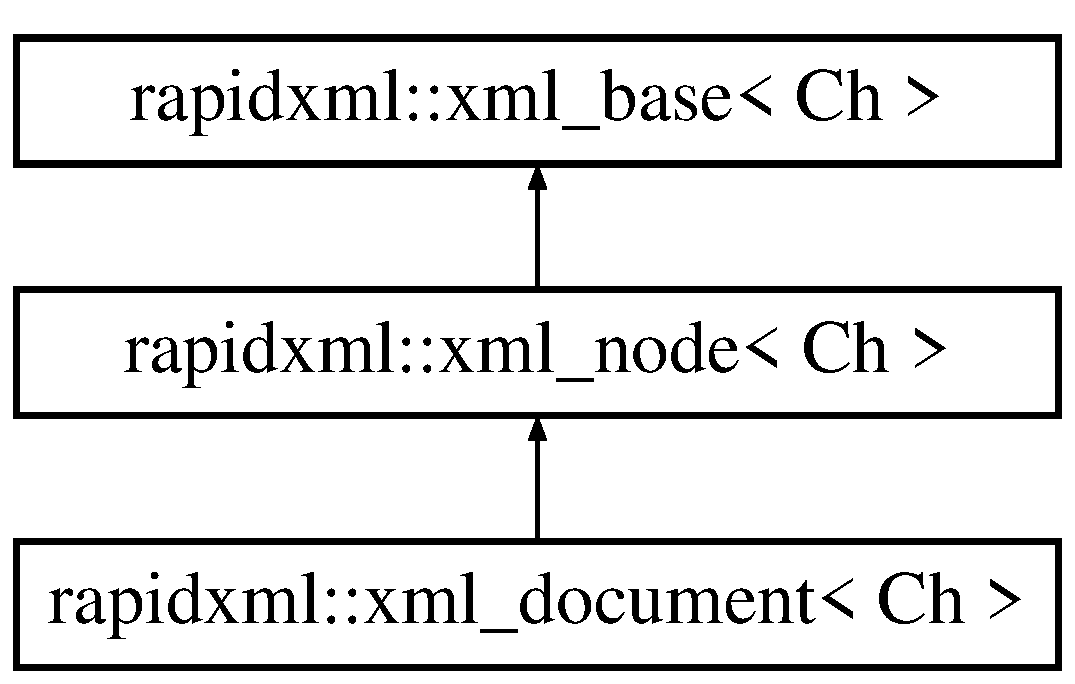
\includegraphics[height=3.000000cm]{classrapidxml_1_1xml__node}
\end{center}
\end{figure}
\subsection*{Public Member Functions}
\begin{DoxyCompactItemize}
\item 
\hyperlink{classrapidxml_1_1xml__node_a8bd9019960b90605a45998b661fb1b0e}{xml\+\_\+node} (\hyperlink{namespacerapidxml_abb456db38f7efb746c4330eed6072a7c}{node\+\_\+type} \hyperlink{classrapidxml_1_1xml__node_a2c6a4315b98bcfa2e04fed3fa1b22c36}{type})
\item 
\hyperlink{namespacerapidxml_abb456db38f7efb746c4330eed6072a7c}{node\+\_\+type} \hyperlink{classrapidxml_1_1xml__node_a2c6a4315b98bcfa2e04fed3fa1b22c36}{type} () const 
\item 
\hyperlink{classrapidxml_1_1xml__document}{xml\+\_\+document}$<$ Ch $>$ $\ast$ \hyperlink{classrapidxml_1_1xml__node_adb6ad21a4590cf13d4a6a5036e3cdbbc}{document} () const 
\item 
\hyperlink{classrapidxml_1_1xml__node}{xml\+\_\+node}$<$ Ch $>$ $\ast$ \hyperlink{classrapidxml_1_1xml__node_a2dedeb4e04bb35e06a9a7bddf6ba652d}{first\+\_\+node} (const Ch $\ast$\hyperlink{classrapidxml_1_1xml__base_a9a09739310469995db078ebd0da3ed45}{name}=0, std\+::size\+\_\+t \hyperlink{classrapidxml_1_1xml__base_a7e7f98b3d01e1eab8dc1ca69aad9af84}{name\+\_\+size}=0, bool case\+\_\+sensitive=true) const 
\item 
\hyperlink{classrapidxml_1_1xml__node}{xml\+\_\+node}$<$ Ch $>$ $\ast$ \hyperlink{classrapidxml_1_1xml__node_a2ace550c18cf10da6303773972d7157f}{last\+\_\+node} (const Ch $\ast$\hyperlink{classrapidxml_1_1xml__base_a9a09739310469995db078ebd0da3ed45}{name}=0, std\+::size\+\_\+t \hyperlink{classrapidxml_1_1xml__base_a7e7f98b3d01e1eab8dc1ca69aad9af84}{name\+\_\+size}=0, bool case\+\_\+sensitive=true) const 
\item 
\hyperlink{classrapidxml_1_1xml__node}{xml\+\_\+node}$<$ Ch $>$ $\ast$ \hyperlink{classrapidxml_1_1xml__node_a001ece4e227eebbd6ad0ec7dacf1c00b}{previous\+\_\+sibling} (const Ch $\ast$\hyperlink{classrapidxml_1_1xml__base_a9a09739310469995db078ebd0da3ed45}{name}=0, std\+::size\+\_\+t \hyperlink{classrapidxml_1_1xml__base_a7e7f98b3d01e1eab8dc1ca69aad9af84}{name\+\_\+size}=0, bool case\+\_\+sensitive=true) const 
\item 
\hyperlink{classrapidxml_1_1xml__node}{xml\+\_\+node}$<$ Ch $>$ $\ast$ \hyperlink{classrapidxml_1_1xml__node_ac59af4dd5f0ec715753e42467dff6aed}{next\+\_\+sibling} (const Ch $\ast$\hyperlink{classrapidxml_1_1xml__base_a9a09739310469995db078ebd0da3ed45}{name}=0, std\+::size\+\_\+t \hyperlink{classrapidxml_1_1xml__base_a7e7f98b3d01e1eab8dc1ca69aad9af84}{name\+\_\+size}=0, bool case\+\_\+sensitive=true) const 
\item 
\hyperlink{classrapidxml_1_1xml__attribute}{xml\+\_\+attribute}$<$ Ch $>$ $\ast$ \hyperlink{classrapidxml_1_1xml__node_ae426802be58114ffc41bf30ac6b8c37d}{first\+\_\+attribute} (const Ch $\ast$\hyperlink{classrapidxml_1_1xml__base_a9a09739310469995db078ebd0da3ed45}{name}=0, std\+::size\+\_\+t \hyperlink{classrapidxml_1_1xml__base_a7e7f98b3d01e1eab8dc1ca69aad9af84}{name\+\_\+size}=0, bool case\+\_\+sensitive=true) const 
\item 
\hyperlink{classrapidxml_1_1xml__attribute}{xml\+\_\+attribute}$<$ Ch $>$ $\ast$ \hyperlink{classrapidxml_1_1xml__node_a50c03f2db3fa51f27a73d86ec29a49d3}{last\+\_\+attribute} (const Ch $\ast$\hyperlink{classrapidxml_1_1xml__base_a9a09739310469995db078ebd0da3ed45}{name}=0, std\+::size\+\_\+t \hyperlink{classrapidxml_1_1xml__base_a7e7f98b3d01e1eab8dc1ca69aad9af84}{name\+\_\+size}=0, bool case\+\_\+sensitive=true) const 
\item 
void \hyperlink{classrapidxml_1_1xml__node_a499bbc9300c1b06821d5c08b24164c68}{type} (\hyperlink{namespacerapidxml_abb456db38f7efb746c4330eed6072a7c}{node\+\_\+type} type)
\item 
void \hyperlink{classrapidxml_1_1xml__node_ae86e92908c3eab40bbed8216e4f3f3cb}{prepend\+\_\+node} (\hyperlink{classrapidxml_1_1xml__node}{xml\+\_\+node}$<$ Ch $>$ $\ast$child)
\item 
void \hyperlink{classrapidxml_1_1xml__node_a8696d098ecc9c4d2a646b43e91d58e31}{append\+\_\+node} (\hyperlink{classrapidxml_1_1xml__node}{xml\+\_\+node}$<$ Ch $>$ $\ast$child)
\item 
void \hyperlink{classrapidxml_1_1xml__node_a666880f42a7e486d78cc45ed51c7c46d}{insert\+\_\+node} (\hyperlink{classrapidxml_1_1xml__node}{xml\+\_\+node}$<$ Ch $>$ $\ast$where, \hyperlink{classrapidxml_1_1xml__node}{xml\+\_\+node}$<$ Ch $>$ $\ast$child)
\item 
void \hyperlink{classrapidxml_1_1xml__node_a62bf7b276cf7a651a3337f5e0a0ef6ac}{remove\+\_\+first\+\_\+node} ()
\item 
void \hyperlink{classrapidxml_1_1xml__node_a9182512e948ec451a83f116cce7c7674}{remove\+\_\+last\+\_\+node} ()
\item 
void \hyperlink{classrapidxml_1_1xml__node_a98289923eb9e8889418a9eb0207ea35c}{remove\+\_\+node} (\hyperlink{classrapidxml_1_1xml__node}{xml\+\_\+node}$<$ Ch $>$ $\ast$where)
\begin{DoxyCompactList}\small\item\em Removes specified child from the node. \end{DoxyCompactList}\item 
void \hyperlink{classrapidxml_1_1xml__node_a95735358b079ae0adcfbbac69aa1fbc3}{remove\+\_\+all\+\_\+nodes} ()
\begin{DoxyCompactList}\small\item\em Removes all child nodes (but not attributes). \end{DoxyCompactList}\item 
void \hyperlink{classrapidxml_1_1xml__node_a8b62ee76489faf8e2d1210869d547684}{prepend\+\_\+attribute} (\hyperlink{classrapidxml_1_1xml__attribute}{xml\+\_\+attribute}$<$ Ch $>$ $\ast$attribute)
\item 
void \hyperlink{classrapidxml_1_1xml__node_a33ce3386f8c42dd4db658b75cbb6e6c4}{append\+\_\+attribute} (\hyperlink{classrapidxml_1_1xml__attribute}{xml\+\_\+attribute}$<$ Ch $>$ $\ast$attribute)
\item 
void \hyperlink{classrapidxml_1_1xml__node_a9fe659cdf4a5b3bbf5e8ffc98db5a84f}{insert\+\_\+attribute} (\hyperlink{classrapidxml_1_1xml__attribute}{xml\+\_\+attribute}$<$ Ch $>$ $\ast$where, \hyperlink{classrapidxml_1_1xml__attribute}{xml\+\_\+attribute}$<$ Ch $>$ $\ast$attribute)
\item 
void \hyperlink{classrapidxml_1_1xml__node_aa95192d2a165cca16c551ed2a2a06aec}{remove\+\_\+first\+\_\+attribute} ()
\item 
void \hyperlink{classrapidxml_1_1xml__node_a1781a2cbedc9a51d609ad5b528125635}{remove\+\_\+last\+\_\+attribute} ()
\item 
void \hyperlink{classrapidxml_1_1xml__node_a6f97b1b4f46a94a4587915df3c0c6b57}{remove\+\_\+attribute} (\hyperlink{classrapidxml_1_1xml__attribute}{xml\+\_\+attribute}$<$ Ch $>$ $\ast$where)
\item 
void \hyperlink{classrapidxml_1_1xml__node_aa8d5d9484aa1eb5ff1841a073c84c1aa}{remove\+\_\+all\+\_\+attributes} ()
\begin{DoxyCompactList}\small\item\em Removes all attributes of node. \end{DoxyCompactList}\item 
Ch $\ast$ \hyperlink{classrapidxml_1_1xml__base_a9a09739310469995db078ebd0da3ed45}{name} () const 
\item 
void \hyperlink{classrapidxml_1_1xml__base_ae55060ae958c6e6465d6c8db852ec6ce}{name} (const Ch $\ast$name, std\+::size\+\_\+t size)
\item 
void \hyperlink{classrapidxml_1_1xml__base_a4611ddc82ac83a527c65606600eb2a0d}{name} (const Ch $\ast$name)
\item 
std\+::size\+\_\+t \hyperlink{classrapidxml_1_1xml__base_a7e7f98b3d01e1eab8dc1ca69aad9af84}{name\+\_\+size} () const 
\item 
Ch $\ast$ \hyperlink{classrapidxml_1_1xml__base_adcdaccff61c665f039d9344e447b7445}{value} () const 
\item 
void \hyperlink{classrapidxml_1_1xml__base_a3b183c2db7022a6d30494dd2f0ac11e9}{value} (const Ch $\ast$value, std\+::size\+\_\+t size)
\item 
void \hyperlink{classrapidxml_1_1xml__base_a81e63ec4bfd2d7ef0a6c2ed49be6e623}{value} (const Ch $\ast$value)
\item 
std\+::size\+\_\+t \hyperlink{classrapidxml_1_1xml__base_a9fcf201ed0915ac18dd43b0b5dcfaf32}{value\+\_\+size} () const 
\item 
\hyperlink{classrapidxml_1_1xml__node}{xml\+\_\+node}$<$ Ch $>$ $\ast$ \hyperlink{classrapidxml_1_1xml__base_a7f31ae930f93852830234db1ae59c4c4}{parent} () const 
\end{DoxyCompactItemize}
\subsection*{Static Protected Member Functions}
\begin{DoxyCompactItemize}
\item 
static Ch $\ast$ \hyperlink{classrapidxml_1_1xml__base_ad96ff6b1e41dab3ff60b9bc4df769a75}{nullstr} ()
\end{DoxyCompactItemize}
\subsection*{Protected Attributes}
\begin{DoxyCompactItemize}
\item 
Ch $\ast$ \hyperlink{classrapidxml_1_1xml__base_afd9851ed43e14619db0d7075ef8e9e8a}{m\+\_\+name}
\item 
Ch $\ast$ \hyperlink{classrapidxml_1_1xml__base_a278a1ea63b0b70219b946cec47fa00ea}{m\+\_\+value}
\item 
std\+::size\+\_\+t \hyperlink{classrapidxml_1_1xml__base_a5a8c76a7274b4180213796422c4df76f}{m\+\_\+name\+\_\+size}
\item 
std\+::size\+\_\+t \hyperlink{classrapidxml_1_1xml__base_aa3a49d8ceddb8a8d7edb773a2226b89c}{m\+\_\+value\+\_\+size}
\item 
\hyperlink{classrapidxml_1_1xml__node}{xml\+\_\+node}$<$ Ch $>$ $\ast$ \hyperlink{classrapidxml_1_1xml__base_a90d5f660f078f66563fd7b2d8387ccb0}{m\+\_\+parent}
\end{DoxyCompactItemize}
\subsection*{Private Member Functions}
\begin{DoxyCompactItemize}
\item 
\hyperlink{classrapidxml_1_1xml__node_af5f365f98059708e7180c0fbcf1412c5}{xml\+\_\+node} (const \hyperlink{classrapidxml_1_1xml__node}{xml\+\_\+node} \&)
\item 
void \hyperlink{classrapidxml_1_1xml__node_aa9320e2dd58cfbe5fe4b43b9f0d8c788}{operator=} (const \hyperlink{classrapidxml_1_1xml__node}{xml\+\_\+node} \&)
\end{DoxyCompactItemize}
\subsection*{Private Attributes}
\begin{DoxyCompactItemize}
\item 
\hyperlink{namespacerapidxml_abb456db38f7efb746c4330eed6072a7c}{node\+\_\+type} \hyperlink{classrapidxml_1_1xml__node_a33912a5ceef221d662bbac67c70e1397}{m\+\_\+type}
\item 
\hyperlink{classrapidxml_1_1xml__node}{xml\+\_\+node}$<$ Ch $>$ $\ast$ \hyperlink{classrapidxml_1_1xml__node_a3c2a0b286724865b5c000e3333f60d4a}{m\+\_\+first\+\_\+node}
\item 
\hyperlink{classrapidxml_1_1xml__node}{xml\+\_\+node}$<$ Ch $>$ $\ast$ \hyperlink{classrapidxml_1_1xml__node_adc211d26cfea2ba6fb51adb27694ff09}{m\+\_\+last\+\_\+node}
\item 
\hyperlink{classrapidxml_1_1xml__attribute}{xml\+\_\+attribute}$<$ Ch $>$ $\ast$ \hyperlink{classrapidxml_1_1xml__node_a5f7caf8d72d8fae634be6eb744ad8538}{m\+\_\+first\+\_\+attribute}
\item 
\hyperlink{classrapidxml_1_1xml__attribute}{xml\+\_\+attribute}$<$ Ch $>$ $\ast$ \hyperlink{classrapidxml_1_1xml__node_ad82c1bdd1a5c94927cf8a627f18953b9}{m\+\_\+last\+\_\+attribute}
\item 
\hyperlink{classrapidxml_1_1xml__node}{xml\+\_\+node}$<$ Ch $>$ $\ast$ \hyperlink{classrapidxml_1_1xml__node_a571f24c86107f8442f46a514a7cc5d0d}{m\+\_\+prev\+\_\+sibling}
\item 
\hyperlink{classrapidxml_1_1xml__node}{xml\+\_\+node}$<$ Ch $>$ $\ast$ \hyperlink{classrapidxml_1_1xml__node_a202e84dfdd34cb65557b64e31b7e205a}{m\+\_\+next\+\_\+sibling}
\end{DoxyCompactItemize}


\subsection{Detailed Description}
\subsubsection*{template$<$class Ch = char$>$class rapidxml\+::xml\+\_\+node$<$ Ch $>$}

Class representing a node of X\+M\+L document. Each node may have associated name and value strings, which are available through \hyperlink{classrapidxml_1_1xml__base_a9a09739310469995db078ebd0da3ed45}{name()} and \hyperlink{classrapidxml_1_1xml__base_adcdaccff61c665f039d9344e447b7445}{value()} functions. Interpretation of name and value depends on type of the node. Type of node can be determined by using \hyperlink{classrapidxml_1_1xml__node_a2c6a4315b98bcfa2e04fed3fa1b22c36}{type()} function. ~\newline
~\newline
 Note that after parse, both name and value of node, if any, will point interior of source text used for parsing. Thus, this text must persist in the memory for the lifetime of node. 
\begin{DoxyParams}{Parameters}
{\em Ch} & Character type to use. \\
\hline
\end{DoxyParams}


\subsection{Constructor \& Destructor Documentation}
\hypertarget{classrapidxml_1_1xml__node_a8bd9019960b90605a45998b661fb1b0e}{}\index{rapidxml\+::xml\+\_\+node@{rapidxml\+::xml\+\_\+node}!xml\+\_\+node@{xml\+\_\+node}}
\index{xml\+\_\+node@{xml\+\_\+node}!rapidxml\+::xml\+\_\+node@{rapidxml\+::xml\+\_\+node}}
\subsubsection[{xml\+\_\+node}]{\setlength{\rightskip}{0pt plus 5cm}template$<$class Ch = char$>$ {\bf rapidxml\+::xml\+\_\+node}$<$ Ch $>$\+::{\bf xml\+\_\+node} (
\begin{DoxyParamCaption}
\item[{{\bf node\+\_\+type}}]{type}
\end{DoxyParamCaption}
)\hspace{0.3cm}{\ttfamily [inline]}}\label{classrapidxml_1_1xml__node_a8bd9019960b90605a45998b661fb1b0e}
Constructs an empty node with the specified type. Consider using \hyperlink{classrapidxml_1_1memory__pool}{memory\+\_\+pool} of appropriate document to allocate nodes manually. 
\begin{DoxyParams}{Parameters}
{\em type} & Type of node to construct. \\
\hline
\end{DoxyParams}
\hypertarget{classrapidxml_1_1xml__node_af5f365f98059708e7180c0fbcf1412c5}{}\index{rapidxml\+::xml\+\_\+node@{rapidxml\+::xml\+\_\+node}!xml\+\_\+node@{xml\+\_\+node}}
\index{xml\+\_\+node@{xml\+\_\+node}!rapidxml\+::xml\+\_\+node@{rapidxml\+::xml\+\_\+node}}
\subsubsection[{xml\+\_\+node}]{\setlength{\rightskip}{0pt plus 5cm}template$<$class Ch = char$>$ {\bf rapidxml\+::xml\+\_\+node}$<$ Ch $>$\+::{\bf xml\+\_\+node} (
\begin{DoxyParamCaption}
\item[{const {\bf xml\+\_\+node}$<$ Ch $>$ \&}]{}
\end{DoxyParamCaption}
)\hspace{0.3cm}{\ttfamily [private]}}\label{classrapidxml_1_1xml__node_af5f365f98059708e7180c0fbcf1412c5}


\subsection{Member Function Documentation}
\hypertarget{classrapidxml_1_1xml__node_a33ce3386f8c42dd4db658b75cbb6e6c4}{}\index{rapidxml\+::xml\+\_\+node@{rapidxml\+::xml\+\_\+node}!append\+\_\+attribute@{append\+\_\+attribute}}
\index{append\+\_\+attribute@{append\+\_\+attribute}!rapidxml\+::xml\+\_\+node@{rapidxml\+::xml\+\_\+node}}
\subsubsection[{append\+\_\+attribute}]{\setlength{\rightskip}{0pt plus 5cm}template$<$class Ch = char$>$ void {\bf rapidxml\+::xml\+\_\+node}$<$ Ch $>$\+::append\+\_\+attribute (
\begin{DoxyParamCaption}
\item[{{\bf xml\+\_\+attribute}$<$ Ch $>$ $\ast$}]{attribute}
\end{DoxyParamCaption}
)\hspace{0.3cm}{\ttfamily [inline]}}\label{classrapidxml_1_1xml__node_a33ce3386f8c42dd4db658b75cbb6e6c4}
Appends a new attribute to the node. 
\begin{DoxyParams}{Parameters}
{\em attribute} & Attribute to append. \\
\hline
\end{DoxyParams}
\hypertarget{classrapidxml_1_1xml__node_a8696d098ecc9c4d2a646b43e91d58e31}{}\index{rapidxml\+::xml\+\_\+node@{rapidxml\+::xml\+\_\+node}!append\+\_\+node@{append\+\_\+node}}
\index{append\+\_\+node@{append\+\_\+node}!rapidxml\+::xml\+\_\+node@{rapidxml\+::xml\+\_\+node}}
\subsubsection[{append\+\_\+node}]{\setlength{\rightskip}{0pt plus 5cm}template$<$class Ch = char$>$ void {\bf rapidxml\+::xml\+\_\+node}$<$ Ch $>$\+::append\+\_\+node (
\begin{DoxyParamCaption}
\item[{{\bf xml\+\_\+node}$<$ Ch $>$ $\ast$}]{child}
\end{DoxyParamCaption}
)\hspace{0.3cm}{\ttfamily [inline]}}\label{classrapidxml_1_1xml__node_a8696d098ecc9c4d2a646b43e91d58e31}
Appends a new child node. The appended child becomes the last child. 
\begin{DoxyParams}{Parameters}
{\em child} & Node to append. \\
\hline
\end{DoxyParams}
\hypertarget{classrapidxml_1_1xml__node_adb6ad21a4590cf13d4a6a5036e3cdbbc}{}\index{rapidxml\+::xml\+\_\+node@{rapidxml\+::xml\+\_\+node}!document@{document}}
\index{document@{document}!rapidxml\+::xml\+\_\+node@{rapidxml\+::xml\+\_\+node}}
\subsubsection[{document}]{\setlength{\rightskip}{0pt plus 5cm}template$<$class Ch = char$>$ {\bf xml\+\_\+document}$<$Ch$>$$\ast$ {\bf rapidxml\+::xml\+\_\+node}$<$ Ch $>$\+::document (
\begin{DoxyParamCaption}
{}
\end{DoxyParamCaption}
) const\hspace{0.3cm}{\ttfamily [inline]}}\label{classrapidxml_1_1xml__node_adb6ad21a4590cf13d4a6a5036e3cdbbc}
Gets document of which node is a child. \begin{DoxyReturn}{Returns}
Pointer to document that contains this node, or 0 if there is no parent document. 
\end{DoxyReturn}
\hypertarget{classrapidxml_1_1xml__node_ae426802be58114ffc41bf30ac6b8c37d}{}\index{rapidxml\+::xml\+\_\+node@{rapidxml\+::xml\+\_\+node}!first\+\_\+attribute@{first\+\_\+attribute}}
\index{first\+\_\+attribute@{first\+\_\+attribute}!rapidxml\+::xml\+\_\+node@{rapidxml\+::xml\+\_\+node}}
\subsubsection[{first\+\_\+attribute}]{\setlength{\rightskip}{0pt plus 5cm}template$<$class Ch = char$>$ {\bf xml\+\_\+attribute}$<$Ch$>$$\ast$ {\bf rapidxml\+::xml\+\_\+node}$<$ Ch $>$\+::first\+\_\+attribute (
\begin{DoxyParamCaption}
\item[{const Ch $\ast$}]{name = {\ttfamily 0}, }
\item[{std\+::size\+\_\+t}]{name\+\_\+size = {\ttfamily 0}, }
\item[{bool}]{case\+\_\+sensitive = {\ttfamily true}}
\end{DoxyParamCaption}
) const\hspace{0.3cm}{\ttfamily [inline]}}\label{classrapidxml_1_1xml__node_ae426802be58114ffc41bf30ac6b8c37d}
Gets first attribute of node, optionally matching attribute name. 
\begin{DoxyParams}{Parameters}
{\em name} & Name of attribute to find, or 0 to return first attribute regardless of its name; this string doesn\textquotesingle{}t have to be zero-\/terminated if name\+\_\+size is non-\/zero \\
\hline
{\em name\+\_\+size} & Size of name, in characters, or 0 to have size calculated automatically from string \\
\hline
{\em case\+\_\+sensitive} & Should name comparison be case-\/sensitive; non case-\/sensitive comparison works properly only for A\+S\+C\+I\+I characters \\
\hline
\end{DoxyParams}
\begin{DoxyReturn}{Returns}
Pointer to found attribute, or 0 if not found. 
\end{DoxyReturn}
\hypertarget{classrapidxml_1_1xml__node_a2dedeb4e04bb35e06a9a7bddf6ba652d}{}\index{rapidxml\+::xml\+\_\+node@{rapidxml\+::xml\+\_\+node}!first\+\_\+node@{first\+\_\+node}}
\index{first\+\_\+node@{first\+\_\+node}!rapidxml\+::xml\+\_\+node@{rapidxml\+::xml\+\_\+node}}
\subsubsection[{first\+\_\+node}]{\setlength{\rightskip}{0pt plus 5cm}template$<$class Ch = char$>$ {\bf xml\+\_\+node}$<$Ch$>$$\ast$ {\bf rapidxml\+::xml\+\_\+node}$<$ Ch $>$\+::first\+\_\+node (
\begin{DoxyParamCaption}
\item[{const Ch $\ast$}]{name = {\ttfamily 0}, }
\item[{std\+::size\+\_\+t}]{name\+\_\+size = {\ttfamily 0}, }
\item[{bool}]{case\+\_\+sensitive = {\ttfamily true}}
\end{DoxyParamCaption}
) const\hspace{0.3cm}{\ttfamily [inline]}}\label{classrapidxml_1_1xml__node_a2dedeb4e04bb35e06a9a7bddf6ba652d}
Gets first child node, optionally matching node name. 
\begin{DoxyParams}{Parameters}
{\em name} & Name of child to find, or 0 to return first child regardless of its name; this string doesn\textquotesingle{}t have to be zero-\/terminated if name\+\_\+size is non-\/zero \\
\hline
{\em name\+\_\+size} & Size of name, in characters, or 0 to have size calculated automatically from string \\
\hline
{\em case\+\_\+sensitive} & Should name comparison be case-\/sensitive; non case-\/sensitive comparison works properly only for A\+S\+C\+I\+I characters \\
\hline
\end{DoxyParams}
\begin{DoxyReturn}{Returns}
Pointer to found child, or 0 if not found. 
\end{DoxyReturn}
\hypertarget{classrapidxml_1_1xml__node_a9fe659cdf4a5b3bbf5e8ffc98db5a84f}{}\index{rapidxml\+::xml\+\_\+node@{rapidxml\+::xml\+\_\+node}!insert\+\_\+attribute@{insert\+\_\+attribute}}
\index{insert\+\_\+attribute@{insert\+\_\+attribute}!rapidxml\+::xml\+\_\+node@{rapidxml\+::xml\+\_\+node}}
\subsubsection[{insert\+\_\+attribute}]{\setlength{\rightskip}{0pt plus 5cm}template$<$class Ch = char$>$ void {\bf rapidxml\+::xml\+\_\+node}$<$ Ch $>$\+::insert\+\_\+attribute (
\begin{DoxyParamCaption}
\item[{{\bf xml\+\_\+attribute}$<$ Ch $>$ $\ast$}]{where, }
\item[{{\bf xml\+\_\+attribute}$<$ Ch $>$ $\ast$}]{attribute}
\end{DoxyParamCaption}
)\hspace{0.3cm}{\ttfamily [inline]}}\label{classrapidxml_1_1xml__node_a9fe659cdf4a5b3bbf5e8ffc98db5a84f}
Inserts a new attribute at specified place inside the node. All attributes after and including the specified attribute are moved one position back. 
\begin{DoxyParams}{Parameters}
{\em where} & Place where to insert the attribute, or 0 to insert at the back. \\
\hline
{\em attribute} & Attribute to insert. \\
\hline
\end{DoxyParams}
\hypertarget{classrapidxml_1_1xml__node_a666880f42a7e486d78cc45ed51c7c46d}{}\index{rapidxml\+::xml\+\_\+node@{rapidxml\+::xml\+\_\+node}!insert\+\_\+node@{insert\+\_\+node}}
\index{insert\+\_\+node@{insert\+\_\+node}!rapidxml\+::xml\+\_\+node@{rapidxml\+::xml\+\_\+node}}
\subsubsection[{insert\+\_\+node}]{\setlength{\rightskip}{0pt plus 5cm}template$<$class Ch = char$>$ void {\bf rapidxml\+::xml\+\_\+node}$<$ Ch $>$\+::insert\+\_\+node (
\begin{DoxyParamCaption}
\item[{{\bf xml\+\_\+node}$<$ Ch $>$ $\ast$}]{where, }
\item[{{\bf xml\+\_\+node}$<$ Ch $>$ $\ast$}]{child}
\end{DoxyParamCaption}
)\hspace{0.3cm}{\ttfamily [inline]}}\label{classrapidxml_1_1xml__node_a666880f42a7e486d78cc45ed51c7c46d}
Inserts a new child node at specified place inside the node. All children after and including the specified node are moved one position back. 
\begin{DoxyParams}{Parameters}
{\em where} & Place where to insert the child, or 0 to insert at the back. \\
\hline
{\em child} & Node to insert. \\
\hline
\end{DoxyParams}
\hypertarget{classrapidxml_1_1xml__node_a50c03f2db3fa51f27a73d86ec29a49d3}{}\index{rapidxml\+::xml\+\_\+node@{rapidxml\+::xml\+\_\+node}!last\+\_\+attribute@{last\+\_\+attribute}}
\index{last\+\_\+attribute@{last\+\_\+attribute}!rapidxml\+::xml\+\_\+node@{rapidxml\+::xml\+\_\+node}}
\subsubsection[{last\+\_\+attribute}]{\setlength{\rightskip}{0pt plus 5cm}template$<$class Ch = char$>$ {\bf xml\+\_\+attribute}$<$Ch$>$$\ast$ {\bf rapidxml\+::xml\+\_\+node}$<$ Ch $>$\+::last\+\_\+attribute (
\begin{DoxyParamCaption}
\item[{const Ch $\ast$}]{name = {\ttfamily 0}, }
\item[{std\+::size\+\_\+t}]{name\+\_\+size = {\ttfamily 0}, }
\item[{bool}]{case\+\_\+sensitive = {\ttfamily true}}
\end{DoxyParamCaption}
) const\hspace{0.3cm}{\ttfamily [inline]}}\label{classrapidxml_1_1xml__node_a50c03f2db3fa51f27a73d86ec29a49d3}
Gets last attribute of node, optionally matching attribute name. 
\begin{DoxyParams}{Parameters}
{\em name} & Name of attribute to find, or 0 to return last attribute regardless of its name; this string doesn\textquotesingle{}t have to be zero-\/terminated if name\+\_\+size is non-\/zero \\
\hline
{\em name\+\_\+size} & Size of name, in characters, or 0 to have size calculated automatically from string \\
\hline
{\em case\+\_\+sensitive} & Should name comparison be case-\/sensitive; non case-\/sensitive comparison works properly only for A\+S\+C\+I\+I characters \\
\hline
\end{DoxyParams}
\begin{DoxyReturn}{Returns}
Pointer to found attribute, or 0 if not found. 
\end{DoxyReturn}
\hypertarget{classrapidxml_1_1xml__node_a2ace550c18cf10da6303773972d7157f}{}\index{rapidxml\+::xml\+\_\+node@{rapidxml\+::xml\+\_\+node}!last\+\_\+node@{last\+\_\+node}}
\index{last\+\_\+node@{last\+\_\+node}!rapidxml\+::xml\+\_\+node@{rapidxml\+::xml\+\_\+node}}
\subsubsection[{last\+\_\+node}]{\setlength{\rightskip}{0pt plus 5cm}template$<$class Ch = char$>$ {\bf xml\+\_\+node}$<$Ch$>$$\ast$ {\bf rapidxml\+::xml\+\_\+node}$<$ Ch $>$\+::last\+\_\+node (
\begin{DoxyParamCaption}
\item[{const Ch $\ast$}]{name = {\ttfamily 0}, }
\item[{std\+::size\+\_\+t}]{name\+\_\+size = {\ttfamily 0}, }
\item[{bool}]{case\+\_\+sensitive = {\ttfamily true}}
\end{DoxyParamCaption}
) const\hspace{0.3cm}{\ttfamily [inline]}}\label{classrapidxml_1_1xml__node_a2ace550c18cf10da6303773972d7157f}
Gets last child node, optionally matching node name. Behaviour is undefined if node has no children. Use \hyperlink{classrapidxml_1_1xml__node_a2dedeb4e04bb35e06a9a7bddf6ba652d}{first\+\_\+node()} to test if node has children. 
\begin{DoxyParams}{Parameters}
{\em name} & Name of child to find, or 0 to return last child regardless of its name; this string doesn\textquotesingle{}t have to be zero-\/terminated if name\+\_\+size is non-\/zero \\
\hline
{\em name\+\_\+size} & Size of name, in characters, or 0 to have size calculated automatically from string \\
\hline
{\em case\+\_\+sensitive} & Should name comparison be case-\/sensitive; non case-\/sensitive comparison works properly only for A\+S\+C\+I\+I characters \\
\hline
\end{DoxyParams}
\begin{DoxyReturn}{Returns}
Pointer to found child, or 0 if not found. 
\end{DoxyReturn}
\hypertarget{classrapidxml_1_1xml__base_a9a09739310469995db078ebd0da3ed45}{}\index{rapidxml\+::xml\+\_\+node@{rapidxml\+::xml\+\_\+node}!name@{name}}
\index{name@{name}!rapidxml\+::xml\+\_\+node@{rapidxml\+::xml\+\_\+node}}
\subsubsection[{name}]{\setlength{\rightskip}{0pt plus 5cm}template$<$class Ch  = char$>$ Ch$\ast$ {\bf rapidxml\+::xml\+\_\+base}$<$ Ch $>$\+::name (
\begin{DoxyParamCaption}
{}
\end{DoxyParamCaption}
) const\hspace{0.3cm}{\ttfamily [inline]}, {\ttfamily [inherited]}}\label{classrapidxml_1_1xml__base_a9a09739310469995db078ebd0da3ed45}
Gets name of the node. Interpretation of name depends on type of node. Note that name will not be zero-\/terminated if \hyperlink{namespacerapidxml_af3fc88ba6bee33482a2db81b1da36ea1}{rapidxml\+::parse\+\_\+no\+\_\+string\+\_\+terminators} option was selected during parse. ~\newline
~\newline
 Use \hyperlink{classrapidxml_1_1xml__base_a7e7f98b3d01e1eab8dc1ca69aad9af84}{name\+\_\+size()} function to determine length of the name. \begin{DoxyReturn}{Returns}
Name of node, or empty string if node has no name. 
\end{DoxyReturn}
\hypertarget{classrapidxml_1_1xml__base_ae55060ae958c6e6465d6c8db852ec6ce}{}\index{rapidxml\+::xml\+\_\+node@{rapidxml\+::xml\+\_\+node}!name@{name}}
\index{name@{name}!rapidxml\+::xml\+\_\+node@{rapidxml\+::xml\+\_\+node}}
\subsubsection[{name}]{\setlength{\rightskip}{0pt plus 5cm}template$<$class Ch  = char$>$ void {\bf rapidxml\+::xml\+\_\+base}$<$ Ch $>$\+::name (
\begin{DoxyParamCaption}
\item[{const Ch $\ast$}]{name, }
\item[{std\+::size\+\_\+t}]{size}
\end{DoxyParamCaption}
)\hspace{0.3cm}{\ttfamily [inline]}, {\ttfamily [inherited]}}\label{classrapidxml_1_1xml__base_ae55060ae958c6e6465d6c8db852ec6ce}
Sets name of node to a non zero-\/terminated string. See ownership\+\_\+of\+\_\+strings. ~\newline
~\newline
 Note that node does not own its name or value, it only stores a pointer to it. It will not delete or otherwise free the pointer on destruction. It is reponsibility of the user to properly manage lifetime of the string. The easiest way to achieve it is to use \hyperlink{classrapidxml_1_1memory__pool}{memory\+\_\+pool} of the document to allocate the string -\/ on destruction of the document the string will be automatically freed. ~\newline
~\newline
 Size of name must be specified separately, because name does not have to be zero terminated. Use \hyperlink{classrapidxml_1_1xml__base_a4611ddc82ac83a527c65606600eb2a0d}{name(const Ch $\ast$)} function to have the length automatically calculated (string must be zero terminated). 
\begin{DoxyParams}{Parameters}
{\em name} & Name of node to set. Does not have to be zero terminated. \\
\hline
{\em size} & Size of name, in characters. This does not include zero terminator, if one is present. \\
\hline
\end{DoxyParams}
\hypertarget{classrapidxml_1_1xml__base_a4611ddc82ac83a527c65606600eb2a0d}{}\index{rapidxml\+::xml\+\_\+node@{rapidxml\+::xml\+\_\+node}!name@{name}}
\index{name@{name}!rapidxml\+::xml\+\_\+node@{rapidxml\+::xml\+\_\+node}}
\subsubsection[{name}]{\setlength{\rightskip}{0pt plus 5cm}template$<$class Ch  = char$>$ void {\bf rapidxml\+::xml\+\_\+base}$<$ Ch $>$\+::name (
\begin{DoxyParamCaption}
\item[{const Ch $\ast$}]{name}
\end{DoxyParamCaption}
)\hspace{0.3cm}{\ttfamily [inline]}, {\ttfamily [inherited]}}\label{classrapidxml_1_1xml__base_a4611ddc82ac83a527c65606600eb2a0d}
Sets name of node to a zero-\/terminated string. See also ownership\+\_\+of\+\_\+strings and \hyperlink{classrapidxml_1_1xml__base_ae55060ae958c6e6465d6c8db852ec6ce}{xml\+\_\+node\+::name(const Ch $\ast$, std\+::size\+\_\+t)}. 
\begin{DoxyParams}{Parameters}
{\em name} & Name of node to set. Must be zero terminated. \\
\hline
\end{DoxyParams}
\hypertarget{classrapidxml_1_1xml__base_a7e7f98b3d01e1eab8dc1ca69aad9af84}{}\index{rapidxml\+::xml\+\_\+node@{rapidxml\+::xml\+\_\+node}!name\+\_\+size@{name\+\_\+size}}
\index{name\+\_\+size@{name\+\_\+size}!rapidxml\+::xml\+\_\+node@{rapidxml\+::xml\+\_\+node}}
\subsubsection[{name\+\_\+size}]{\setlength{\rightskip}{0pt plus 5cm}template$<$class Ch  = char$>$ std\+::size\+\_\+t {\bf rapidxml\+::xml\+\_\+base}$<$ Ch $>$\+::name\+\_\+size (
\begin{DoxyParamCaption}
{}
\end{DoxyParamCaption}
) const\hspace{0.3cm}{\ttfamily [inline]}, {\ttfamily [inherited]}}\label{classrapidxml_1_1xml__base_a7e7f98b3d01e1eab8dc1ca69aad9af84}
Gets size of node name, not including terminator character. This function works correctly irrespective of whether name is or is not zero terminated. \begin{DoxyReturn}{Returns}
Size of node name, in characters. 
\end{DoxyReturn}
\hypertarget{classrapidxml_1_1xml__node_ac59af4dd5f0ec715753e42467dff6aed}{}\index{rapidxml\+::xml\+\_\+node@{rapidxml\+::xml\+\_\+node}!next\+\_\+sibling@{next\+\_\+sibling}}
\index{next\+\_\+sibling@{next\+\_\+sibling}!rapidxml\+::xml\+\_\+node@{rapidxml\+::xml\+\_\+node}}
\subsubsection[{next\+\_\+sibling}]{\setlength{\rightskip}{0pt plus 5cm}template$<$class Ch = char$>$ {\bf xml\+\_\+node}$<$Ch$>$$\ast$ {\bf rapidxml\+::xml\+\_\+node}$<$ Ch $>$\+::next\+\_\+sibling (
\begin{DoxyParamCaption}
\item[{const Ch $\ast$}]{name = {\ttfamily 0}, }
\item[{std\+::size\+\_\+t}]{name\+\_\+size = {\ttfamily 0}, }
\item[{bool}]{case\+\_\+sensitive = {\ttfamily true}}
\end{DoxyParamCaption}
) const\hspace{0.3cm}{\ttfamily [inline]}}\label{classrapidxml_1_1xml__node_ac59af4dd5f0ec715753e42467dff6aed}
Gets next sibling node, optionally matching node name. Behaviour is undefined if node has no parent. Use \hyperlink{classrapidxml_1_1xml__base_a7f31ae930f93852830234db1ae59c4c4}{parent()} to test if node has a parent. 
\begin{DoxyParams}{Parameters}
{\em name} & Name of sibling to find, or 0 to return next sibling regardless of its name; this string doesn\textquotesingle{}t have to be zero-\/terminated if name\+\_\+size is non-\/zero \\
\hline
{\em name\+\_\+size} & Size of name, in characters, or 0 to have size calculated automatically from string \\
\hline
{\em case\+\_\+sensitive} & Should name comparison be case-\/sensitive; non case-\/sensitive comparison works properly only for A\+S\+C\+I\+I characters \\
\hline
\end{DoxyParams}
\begin{DoxyReturn}{Returns}
Pointer to found sibling, or 0 if not found. 
\end{DoxyReturn}
\hypertarget{classrapidxml_1_1xml__base_ad96ff6b1e41dab3ff60b9bc4df769a75}{}\index{rapidxml\+::xml\+\_\+node@{rapidxml\+::xml\+\_\+node}!nullstr@{nullstr}}
\index{nullstr@{nullstr}!rapidxml\+::xml\+\_\+node@{rapidxml\+::xml\+\_\+node}}
\subsubsection[{nullstr}]{\setlength{\rightskip}{0pt plus 5cm}template$<$class Ch  = char$>$ static Ch$\ast$ {\bf rapidxml\+::xml\+\_\+base}$<$ Ch $>$\+::nullstr (
\begin{DoxyParamCaption}
{}
\end{DoxyParamCaption}
)\hspace{0.3cm}{\ttfamily [inline]}, {\ttfamily [static]}, {\ttfamily [protected]}, {\ttfamily [inherited]}}\label{classrapidxml_1_1xml__base_ad96ff6b1e41dab3ff60b9bc4df769a75}
\hypertarget{classrapidxml_1_1xml__node_aa9320e2dd58cfbe5fe4b43b9f0d8c788}{}\index{rapidxml\+::xml\+\_\+node@{rapidxml\+::xml\+\_\+node}!operator=@{operator=}}
\index{operator=@{operator=}!rapidxml\+::xml\+\_\+node@{rapidxml\+::xml\+\_\+node}}
\subsubsection[{operator=}]{\setlength{\rightskip}{0pt plus 5cm}template$<$class Ch = char$>$ void {\bf rapidxml\+::xml\+\_\+node}$<$ Ch $>$\+::operator= (
\begin{DoxyParamCaption}
\item[{const {\bf xml\+\_\+node}$<$ Ch $>$ \&}]{}
\end{DoxyParamCaption}
)\hspace{0.3cm}{\ttfamily [private]}}\label{classrapidxml_1_1xml__node_aa9320e2dd58cfbe5fe4b43b9f0d8c788}
\hypertarget{classrapidxml_1_1xml__base_a7f31ae930f93852830234db1ae59c4c4}{}\index{rapidxml\+::xml\+\_\+node@{rapidxml\+::xml\+\_\+node}!parent@{parent}}
\index{parent@{parent}!rapidxml\+::xml\+\_\+node@{rapidxml\+::xml\+\_\+node}}
\subsubsection[{parent}]{\setlength{\rightskip}{0pt plus 5cm}template$<$class Ch  = char$>$ {\bf xml\+\_\+node}$<$Ch$>$$\ast$ {\bf rapidxml\+::xml\+\_\+base}$<$ Ch $>$\+::parent (
\begin{DoxyParamCaption}
{}
\end{DoxyParamCaption}
) const\hspace{0.3cm}{\ttfamily [inline]}, {\ttfamily [inherited]}}\label{classrapidxml_1_1xml__base_a7f31ae930f93852830234db1ae59c4c4}
Gets node parent. \begin{DoxyReturn}{Returns}
Pointer to parent node, or 0 if there is no parent. 
\end{DoxyReturn}
\hypertarget{classrapidxml_1_1xml__node_a8b62ee76489faf8e2d1210869d547684}{}\index{rapidxml\+::xml\+\_\+node@{rapidxml\+::xml\+\_\+node}!prepend\+\_\+attribute@{prepend\+\_\+attribute}}
\index{prepend\+\_\+attribute@{prepend\+\_\+attribute}!rapidxml\+::xml\+\_\+node@{rapidxml\+::xml\+\_\+node}}
\subsubsection[{prepend\+\_\+attribute}]{\setlength{\rightskip}{0pt plus 5cm}template$<$class Ch = char$>$ void {\bf rapidxml\+::xml\+\_\+node}$<$ Ch $>$\+::prepend\+\_\+attribute (
\begin{DoxyParamCaption}
\item[{{\bf xml\+\_\+attribute}$<$ Ch $>$ $\ast$}]{attribute}
\end{DoxyParamCaption}
)\hspace{0.3cm}{\ttfamily [inline]}}\label{classrapidxml_1_1xml__node_a8b62ee76489faf8e2d1210869d547684}
Prepends a new attribute to the node. 
\begin{DoxyParams}{Parameters}
{\em attribute} & Attribute to prepend. \\
\hline
\end{DoxyParams}
\hypertarget{classrapidxml_1_1xml__node_ae86e92908c3eab40bbed8216e4f3f3cb}{}\index{rapidxml\+::xml\+\_\+node@{rapidxml\+::xml\+\_\+node}!prepend\+\_\+node@{prepend\+\_\+node}}
\index{prepend\+\_\+node@{prepend\+\_\+node}!rapidxml\+::xml\+\_\+node@{rapidxml\+::xml\+\_\+node}}
\subsubsection[{prepend\+\_\+node}]{\setlength{\rightskip}{0pt plus 5cm}template$<$class Ch = char$>$ void {\bf rapidxml\+::xml\+\_\+node}$<$ Ch $>$\+::prepend\+\_\+node (
\begin{DoxyParamCaption}
\item[{{\bf xml\+\_\+node}$<$ Ch $>$ $\ast$}]{child}
\end{DoxyParamCaption}
)\hspace{0.3cm}{\ttfamily [inline]}}\label{classrapidxml_1_1xml__node_ae86e92908c3eab40bbed8216e4f3f3cb}
Prepends a new child node. The prepended child becomes the first child, and all existing children are moved one position back. 
\begin{DoxyParams}{Parameters}
{\em child} & Node to prepend. \\
\hline
\end{DoxyParams}
\hypertarget{classrapidxml_1_1xml__node_a001ece4e227eebbd6ad0ec7dacf1c00b}{}\index{rapidxml\+::xml\+\_\+node@{rapidxml\+::xml\+\_\+node}!previous\+\_\+sibling@{previous\+\_\+sibling}}
\index{previous\+\_\+sibling@{previous\+\_\+sibling}!rapidxml\+::xml\+\_\+node@{rapidxml\+::xml\+\_\+node}}
\subsubsection[{previous\+\_\+sibling}]{\setlength{\rightskip}{0pt plus 5cm}template$<$class Ch = char$>$ {\bf xml\+\_\+node}$<$Ch$>$$\ast$ {\bf rapidxml\+::xml\+\_\+node}$<$ Ch $>$\+::previous\+\_\+sibling (
\begin{DoxyParamCaption}
\item[{const Ch $\ast$}]{name = {\ttfamily 0}, }
\item[{std\+::size\+\_\+t}]{name\+\_\+size = {\ttfamily 0}, }
\item[{bool}]{case\+\_\+sensitive = {\ttfamily true}}
\end{DoxyParamCaption}
) const\hspace{0.3cm}{\ttfamily [inline]}}\label{classrapidxml_1_1xml__node_a001ece4e227eebbd6ad0ec7dacf1c00b}
Gets previous sibling node, optionally matching node name. Behaviour is undefined if node has no parent. Use \hyperlink{classrapidxml_1_1xml__base_a7f31ae930f93852830234db1ae59c4c4}{parent()} to test if node has a parent. 
\begin{DoxyParams}{Parameters}
{\em name} & Name of sibling to find, or 0 to return previous sibling regardless of its name; this string doesn\textquotesingle{}t have to be zero-\/terminated if name\+\_\+size is non-\/zero \\
\hline
{\em name\+\_\+size} & Size of name, in characters, or 0 to have size calculated automatically from string \\
\hline
{\em case\+\_\+sensitive} & Should name comparison be case-\/sensitive; non case-\/sensitive comparison works properly only for A\+S\+C\+I\+I characters \\
\hline
\end{DoxyParams}
\begin{DoxyReturn}{Returns}
Pointer to found sibling, or 0 if not found. 
\end{DoxyReturn}
\hypertarget{classrapidxml_1_1xml__node_aa8d5d9484aa1eb5ff1841a073c84c1aa}{}\index{rapidxml\+::xml\+\_\+node@{rapidxml\+::xml\+\_\+node}!remove\+\_\+all\+\_\+attributes@{remove\+\_\+all\+\_\+attributes}}
\index{remove\+\_\+all\+\_\+attributes@{remove\+\_\+all\+\_\+attributes}!rapidxml\+::xml\+\_\+node@{rapidxml\+::xml\+\_\+node}}
\subsubsection[{remove\+\_\+all\+\_\+attributes}]{\setlength{\rightskip}{0pt plus 5cm}template$<$class Ch = char$>$ void {\bf rapidxml\+::xml\+\_\+node}$<$ Ch $>$\+::remove\+\_\+all\+\_\+attributes (
\begin{DoxyParamCaption}
{}
\end{DoxyParamCaption}
)\hspace{0.3cm}{\ttfamily [inline]}}\label{classrapidxml_1_1xml__node_aa8d5d9484aa1eb5ff1841a073c84c1aa}


Removes all attributes of node. 

\hypertarget{classrapidxml_1_1xml__node_a95735358b079ae0adcfbbac69aa1fbc3}{}\index{rapidxml\+::xml\+\_\+node@{rapidxml\+::xml\+\_\+node}!remove\+\_\+all\+\_\+nodes@{remove\+\_\+all\+\_\+nodes}}
\index{remove\+\_\+all\+\_\+nodes@{remove\+\_\+all\+\_\+nodes}!rapidxml\+::xml\+\_\+node@{rapidxml\+::xml\+\_\+node}}
\subsubsection[{remove\+\_\+all\+\_\+nodes}]{\setlength{\rightskip}{0pt plus 5cm}template$<$class Ch = char$>$ void {\bf rapidxml\+::xml\+\_\+node}$<$ Ch $>$\+::remove\+\_\+all\+\_\+nodes (
\begin{DoxyParamCaption}
{}
\end{DoxyParamCaption}
)\hspace{0.3cm}{\ttfamily [inline]}}\label{classrapidxml_1_1xml__node_a95735358b079ae0adcfbbac69aa1fbc3}


Removes all child nodes (but not attributes). 

\hypertarget{classrapidxml_1_1xml__node_a6f97b1b4f46a94a4587915df3c0c6b57}{}\index{rapidxml\+::xml\+\_\+node@{rapidxml\+::xml\+\_\+node}!remove\+\_\+attribute@{remove\+\_\+attribute}}
\index{remove\+\_\+attribute@{remove\+\_\+attribute}!rapidxml\+::xml\+\_\+node@{rapidxml\+::xml\+\_\+node}}
\subsubsection[{remove\+\_\+attribute}]{\setlength{\rightskip}{0pt plus 5cm}template$<$class Ch = char$>$ void {\bf rapidxml\+::xml\+\_\+node}$<$ Ch $>$\+::remove\+\_\+attribute (
\begin{DoxyParamCaption}
\item[{{\bf xml\+\_\+attribute}$<$ Ch $>$ $\ast$}]{where}
\end{DoxyParamCaption}
)\hspace{0.3cm}{\ttfamily [inline]}}\label{classrapidxml_1_1xml__node_a6f97b1b4f46a94a4587915df3c0c6b57}
Removes specified attribute from node. 
\begin{DoxyParams}{Parameters}
{\em where} & Pointer to attribute to be removed. \\
\hline
\end{DoxyParams}
\hypertarget{classrapidxml_1_1xml__node_aa95192d2a165cca16c551ed2a2a06aec}{}\index{rapidxml\+::xml\+\_\+node@{rapidxml\+::xml\+\_\+node}!remove\+\_\+first\+\_\+attribute@{remove\+\_\+first\+\_\+attribute}}
\index{remove\+\_\+first\+\_\+attribute@{remove\+\_\+first\+\_\+attribute}!rapidxml\+::xml\+\_\+node@{rapidxml\+::xml\+\_\+node}}
\subsubsection[{remove\+\_\+first\+\_\+attribute}]{\setlength{\rightskip}{0pt plus 5cm}template$<$class Ch = char$>$ void {\bf rapidxml\+::xml\+\_\+node}$<$ Ch $>$\+::remove\+\_\+first\+\_\+attribute (
\begin{DoxyParamCaption}
{}
\end{DoxyParamCaption}
)\hspace{0.3cm}{\ttfamily [inline]}}\label{classrapidxml_1_1xml__node_aa95192d2a165cca16c551ed2a2a06aec}
Removes first attribute of the node. If node has no attributes, behaviour is undefined. Use \hyperlink{classrapidxml_1_1xml__node_ae426802be58114ffc41bf30ac6b8c37d}{first\+\_\+attribute()} to test if node has attributes. \hypertarget{classrapidxml_1_1xml__node_a62bf7b276cf7a651a3337f5e0a0ef6ac}{}\index{rapidxml\+::xml\+\_\+node@{rapidxml\+::xml\+\_\+node}!remove\+\_\+first\+\_\+node@{remove\+\_\+first\+\_\+node}}
\index{remove\+\_\+first\+\_\+node@{remove\+\_\+first\+\_\+node}!rapidxml\+::xml\+\_\+node@{rapidxml\+::xml\+\_\+node}}
\subsubsection[{remove\+\_\+first\+\_\+node}]{\setlength{\rightskip}{0pt plus 5cm}template$<$class Ch = char$>$ void {\bf rapidxml\+::xml\+\_\+node}$<$ Ch $>$\+::remove\+\_\+first\+\_\+node (
\begin{DoxyParamCaption}
{}
\end{DoxyParamCaption}
)\hspace{0.3cm}{\ttfamily [inline]}}\label{classrapidxml_1_1xml__node_a62bf7b276cf7a651a3337f5e0a0ef6ac}
Removes first child node. If node has no children, behaviour is undefined. Use \hyperlink{classrapidxml_1_1xml__node_a2dedeb4e04bb35e06a9a7bddf6ba652d}{first\+\_\+node()} to test if node has children. \hypertarget{classrapidxml_1_1xml__node_a1781a2cbedc9a51d609ad5b528125635}{}\index{rapidxml\+::xml\+\_\+node@{rapidxml\+::xml\+\_\+node}!remove\+\_\+last\+\_\+attribute@{remove\+\_\+last\+\_\+attribute}}
\index{remove\+\_\+last\+\_\+attribute@{remove\+\_\+last\+\_\+attribute}!rapidxml\+::xml\+\_\+node@{rapidxml\+::xml\+\_\+node}}
\subsubsection[{remove\+\_\+last\+\_\+attribute}]{\setlength{\rightskip}{0pt plus 5cm}template$<$class Ch = char$>$ void {\bf rapidxml\+::xml\+\_\+node}$<$ Ch $>$\+::remove\+\_\+last\+\_\+attribute (
\begin{DoxyParamCaption}
{}
\end{DoxyParamCaption}
)\hspace{0.3cm}{\ttfamily [inline]}}\label{classrapidxml_1_1xml__node_a1781a2cbedc9a51d609ad5b528125635}
Removes last attribute of the node. If node has no attributes, behaviour is undefined. Use \hyperlink{classrapidxml_1_1xml__node_ae426802be58114ffc41bf30ac6b8c37d}{first\+\_\+attribute()} to test if node has attributes. \hypertarget{classrapidxml_1_1xml__node_a9182512e948ec451a83f116cce7c7674}{}\index{rapidxml\+::xml\+\_\+node@{rapidxml\+::xml\+\_\+node}!remove\+\_\+last\+\_\+node@{remove\+\_\+last\+\_\+node}}
\index{remove\+\_\+last\+\_\+node@{remove\+\_\+last\+\_\+node}!rapidxml\+::xml\+\_\+node@{rapidxml\+::xml\+\_\+node}}
\subsubsection[{remove\+\_\+last\+\_\+node}]{\setlength{\rightskip}{0pt plus 5cm}template$<$class Ch = char$>$ void {\bf rapidxml\+::xml\+\_\+node}$<$ Ch $>$\+::remove\+\_\+last\+\_\+node (
\begin{DoxyParamCaption}
{}
\end{DoxyParamCaption}
)\hspace{0.3cm}{\ttfamily [inline]}}\label{classrapidxml_1_1xml__node_a9182512e948ec451a83f116cce7c7674}
Removes last child of the node. If node has no children, behaviour is undefined. Use \hyperlink{classrapidxml_1_1xml__node_a2dedeb4e04bb35e06a9a7bddf6ba652d}{first\+\_\+node()} to test if node has children. \hypertarget{classrapidxml_1_1xml__node_a98289923eb9e8889418a9eb0207ea35c}{}\index{rapidxml\+::xml\+\_\+node@{rapidxml\+::xml\+\_\+node}!remove\+\_\+node@{remove\+\_\+node}}
\index{remove\+\_\+node@{remove\+\_\+node}!rapidxml\+::xml\+\_\+node@{rapidxml\+::xml\+\_\+node}}
\subsubsection[{remove\+\_\+node}]{\setlength{\rightskip}{0pt plus 5cm}template$<$class Ch = char$>$ void {\bf rapidxml\+::xml\+\_\+node}$<$ Ch $>$\+::remove\+\_\+node (
\begin{DoxyParamCaption}
\item[{{\bf xml\+\_\+node}$<$ Ch $>$ $\ast$}]{where}
\end{DoxyParamCaption}
)\hspace{0.3cm}{\ttfamily [inline]}}\label{classrapidxml_1_1xml__node_a98289923eb9e8889418a9eb0207ea35c}


Removes specified child from the node. 

\hypertarget{classrapidxml_1_1xml__node_a2c6a4315b98bcfa2e04fed3fa1b22c36}{}\index{rapidxml\+::xml\+\_\+node@{rapidxml\+::xml\+\_\+node}!type@{type}}
\index{type@{type}!rapidxml\+::xml\+\_\+node@{rapidxml\+::xml\+\_\+node}}
\subsubsection[{type}]{\setlength{\rightskip}{0pt plus 5cm}template$<$class Ch = char$>$ {\bf node\+\_\+type} {\bf rapidxml\+::xml\+\_\+node}$<$ Ch $>$\+::type (
\begin{DoxyParamCaption}
{}
\end{DoxyParamCaption}
) const\hspace{0.3cm}{\ttfamily [inline]}}\label{classrapidxml_1_1xml__node_a2c6a4315b98bcfa2e04fed3fa1b22c36}
Gets type of node. \begin{DoxyReturn}{Returns}
Type of node. 
\end{DoxyReturn}
\hypertarget{classrapidxml_1_1xml__node_a499bbc9300c1b06821d5c08b24164c68}{}\index{rapidxml\+::xml\+\_\+node@{rapidxml\+::xml\+\_\+node}!type@{type}}
\index{type@{type}!rapidxml\+::xml\+\_\+node@{rapidxml\+::xml\+\_\+node}}
\subsubsection[{type}]{\setlength{\rightskip}{0pt plus 5cm}template$<$class Ch = char$>$ void {\bf rapidxml\+::xml\+\_\+node}$<$ Ch $>$\+::type (
\begin{DoxyParamCaption}
\item[{{\bf node\+\_\+type}}]{type}
\end{DoxyParamCaption}
)\hspace{0.3cm}{\ttfamily [inline]}}\label{classrapidxml_1_1xml__node_a499bbc9300c1b06821d5c08b24164c68}
Sets type of node. 
\begin{DoxyParams}{Parameters}
{\em type} & Type of node to set. \\
\hline
\end{DoxyParams}
\hypertarget{classrapidxml_1_1xml__base_adcdaccff61c665f039d9344e447b7445}{}\index{rapidxml\+::xml\+\_\+node@{rapidxml\+::xml\+\_\+node}!value@{value}}
\index{value@{value}!rapidxml\+::xml\+\_\+node@{rapidxml\+::xml\+\_\+node}}
\subsubsection[{value}]{\setlength{\rightskip}{0pt plus 5cm}template$<$class Ch  = char$>$ Ch$\ast$ {\bf rapidxml\+::xml\+\_\+base}$<$ Ch $>$\+::value (
\begin{DoxyParamCaption}
{}
\end{DoxyParamCaption}
) const\hspace{0.3cm}{\ttfamily [inline]}, {\ttfamily [inherited]}}\label{classrapidxml_1_1xml__base_adcdaccff61c665f039d9344e447b7445}
Gets value of node. Interpretation of value depends on type of node. Note that value will not be zero-\/terminated if \hyperlink{namespacerapidxml_af3fc88ba6bee33482a2db81b1da36ea1}{rapidxml\+::parse\+\_\+no\+\_\+string\+\_\+terminators} option was selected during parse. ~\newline
~\newline
 Use \hyperlink{classrapidxml_1_1xml__base_a9fcf201ed0915ac18dd43b0b5dcfaf32}{value\+\_\+size()} function to determine length of the value. \begin{DoxyReturn}{Returns}
Value of node, or empty string if node has no value. 
\end{DoxyReturn}
\hypertarget{classrapidxml_1_1xml__base_a3b183c2db7022a6d30494dd2f0ac11e9}{}\index{rapidxml\+::xml\+\_\+node@{rapidxml\+::xml\+\_\+node}!value@{value}}
\index{value@{value}!rapidxml\+::xml\+\_\+node@{rapidxml\+::xml\+\_\+node}}
\subsubsection[{value}]{\setlength{\rightskip}{0pt plus 5cm}template$<$class Ch  = char$>$ void {\bf rapidxml\+::xml\+\_\+base}$<$ Ch $>$\+::value (
\begin{DoxyParamCaption}
\item[{const Ch $\ast$}]{value, }
\item[{std\+::size\+\_\+t}]{size}
\end{DoxyParamCaption}
)\hspace{0.3cm}{\ttfamily [inline]}, {\ttfamily [inherited]}}\label{classrapidxml_1_1xml__base_a3b183c2db7022a6d30494dd2f0ac11e9}
Sets value of node to a non zero-\/terminated string. See ownership\+\_\+of\+\_\+strings. ~\newline
~\newline
 Note that node does not own its name or value, it only stores a pointer to it. It will not delete or otherwise free the pointer on destruction. It is reponsibility of the user to properly manage lifetime of the string. The easiest way to achieve it is to use \hyperlink{classrapidxml_1_1memory__pool}{memory\+\_\+pool} of the document to allocate the string -\/ on destruction of the document the string will be automatically freed. ~\newline
~\newline
 Size of value must be specified separately, because it does not have to be zero terminated. Use \hyperlink{classrapidxml_1_1xml__base_a81e63ec4bfd2d7ef0a6c2ed49be6e623}{value(const Ch $\ast$)} function to have the length automatically calculated (string must be zero terminated). ~\newline
~\newline
 If an element has a child node of type node\+\_\+data, it will take precedence over element value when printing. If you want to manipulate data of elements using values, use parser flag \hyperlink{namespacerapidxml_ac2d21ef14a4e8936b94aca5d38b1a74d}{rapidxml\+::parse\+\_\+no\+\_\+data\+\_\+nodes} to prevent creation of data nodes by the parser. 
\begin{DoxyParams}{Parameters}
{\em value} & value of node to set. Does not have to be zero terminated. \\
\hline
{\em size} & Size of value, in characters. This does not include zero terminator, if one is present. \\
\hline
\end{DoxyParams}
\hypertarget{classrapidxml_1_1xml__base_a81e63ec4bfd2d7ef0a6c2ed49be6e623}{}\index{rapidxml\+::xml\+\_\+node@{rapidxml\+::xml\+\_\+node}!value@{value}}
\index{value@{value}!rapidxml\+::xml\+\_\+node@{rapidxml\+::xml\+\_\+node}}
\subsubsection[{value}]{\setlength{\rightskip}{0pt plus 5cm}template$<$class Ch  = char$>$ void {\bf rapidxml\+::xml\+\_\+base}$<$ Ch $>$\+::value (
\begin{DoxyParamCaption}
\item[{const Ch $\ast$}]{value}
\end{DoxyParamCaption}
)\hspace{0.3cm}{\ttfamily [inline]}, {\ttfamily [inherited]}}\label{classrapidxml_1_1xml__base_a81e63ec4bfd2d7ef0a6c2ed49be6e623}
Sets value of node to a zero-\/terminated string. See also ownership\+\_\+of\+\_\+strings and \hyperlink{classrapidxml_1_1xml__base_a3b183c2db7022a6d30494dd2f0ac11e9}{xml\+\_\+node\+::value(const Ch $\ast$, std\+::size\+\_\+t)}. 
\begin{DoxyParams}{Parameters}
{\em value} & Vame of node to set. Must be zero terminated. \\
\hline
\end{DoxyParams}
\hypertarget{classrapidxml_1_1xml__base_a9fcf201ed0915ac18dd43b0b5dcfaf32}{}\index{rapidxml\+::xml\+\_\+node@{rapidxml\+::xml\+\_\+node}!value\+\_\+size@{value\+\_\+size}}
\index{value\+\_\+size@{value\+\_\+size}!rapidxml\+::xml\+\_\+node@{rapidxml\+::xml\+\_\+node}}
\subsubsection[{value\+\_\+size}]{\setlength{\rightskip}{0pt plus 5cm}template$<$class Ch  = char$>$ std\+::size\+\_\+t {\bf rapidxml\+::xml\+\_\+base}$<$ Ch $>$\+::value\+\_\+size (
\begin{DoxyParamCaption}
{}
\end{DoxyParamCaption}
) const\hspace{0.3cm}{\ttfamily [inline]}, {\ttfamily [inherited]}}\label{classrapidxml_1_1xml__base_a9fcf201ed0915ac18dd43b0b5dcfaf32}
Gets size of node value, not including terminator character. This function works correctly irrespective of whether value is or is not zero terminated. \begin{DoxyReturn}{Returns}
Size of node value, in characters. 
\end{DoxyReturn}


\subsection{Member Data Documentation}
\hypertarget{classrapidxml_1_1xml__node_a5f7caf8d72d8fae634be6eb744ad8538}{}\index{rapidxml\+::xml\+\_\+node@{rapidxml\+::xml\+\_\+node}!m\+\_\+first\+\_\+attribute@{m\+\_\+first\+\_\+attribute}}
\index{m\+\_\+first\+\_\+attribute@{m\+\_\+first\+\_\+attribute}!rapidxml\+::xml\+\_\+node@{rapidxml\+::xml\+\_\+node}}
\subsubsection[{m\+\_\+first\+\_\+attribute}]{\setlength{\rightskip}{0pt plus 5cm}template$<$class Ch = char$>$ {\bf xml\+\_\+attribute}$<$Ch$>$$\ast$ {\bf rapidxml\+::xml\+\_\+node}$<$ Ch $>$\+::m\+\_\+first\+\_\+attribute\hspace{0.3cm}{\ttfamily [private]}}\label{classrapidxml_1_1xml__node_a5f7caf8d72d8fae634be6eb744ad8538}
\hypertarget{classrapidxml_1_1xml__node_a3c2a0b286724865b5c000e3333f60d4a}{}\index{rapidxml\+::xml\+\_\+node@{rapidxml\+::xml\+\_\+node}!m\+\_\+first\+\_\+node@{m\+\_\+first\+\_\+node}}
\index{m\+\_\+first\+\_\+node@{m\+\_\+first\+\_\+node}!rapidxml\+::xml\+\_\+node@{rapidxml\+::xml\+\_\+node}}
\subsubsection[{m\+\_\+first\+\_\+node}]{\setlength{\rightskip}{0pt plus 5cm}template$<$class Ch = char$>$ {\bf xml\+\_\+node}$<$Ch$>$$\ast$ {\bf rapidxml\+::xml\+\_\+node}$<$ Ch $>$\+::m\+\_\+first\+\_\+node\hspace{0.3cm}{\ttfamily [private]}}\label{classrapidxml_1_1xml__node_a3c2a0b286724865b5c000e3333f60d4a}
\hypertarget{classrapidxml_1_1xml__node_ad82c1bdd1a5c94927cf8a627f18953b9}{}\index{rapidxml\+::xml\+\_\+node@{rapidxml\+::xml\+\_\+node}!m\+\_\+last\+\_\+attribute@{m\+\_\+last\+\_\+attribute}}
\index{m\+\_\+last\+\_\+attribute@{m\+\_\+last\+\_\+attribute}!rapidxml\+::xml\+\_\+node@{rapidxml\+::xml\+\_\+node}}
\subsubsection[{m\+\_\+last\+\_\+attribute}]{\setlength{\rightskip}{0pt plus 5cm}template$<$class Ch = char$>$ {\bf xml\+\_\+attribute}$<$Ch$>$$\ast$ {\bf rapidxml\+::xml\+\_\+node}$<$ Ch $>$\+::m\+\_\+last\+\_\+attribute\hspace{0.3cm}{\ttfamily [private]}}\label{classrapidxml_1_1xml__node_ad82c1bdd1a5c94927cf8a627f18953b9}
\hypertarget{classrapidxml_1_1xml__node_adc211d26cfea2ba6fb51adb27694ff09}{}\index{rapidxml\+::xml\+\_\+node@{rapidxml\+::xml\+\_\+node}!m\+\_\+last\+\_\+node@{m\+\_\+last\+\_\+node}}
\index{m\+\_\+last\+\_\+node@{m\+\_\+last\+\_\+node}!rapidxml\+::xml\+\_\+node@{rapidxml\+::xml\+\_\+node}}
\subsubsection[{m\+\_\+last\+\_\+node}]{\setlength{\rightskip}{0pt plus 5cm}template$<$class Ch = char$>$ {\bf xml\+\_\+node}$<$Ch$>$$\ast$ {\bf rapidxml\+::xml\+\_\+node}$<$ Ch $>$\+::m\+\_\+last\+\_\+node\hspace{0.3cm}{\ttfamily [private]}}\label{classrapidxml_1_1xml__node_adc211d26cfea2ba6fb51adb27694ff09}
\hypertarget{classrapidxml_1_1xml__base_afd9851ed43e14619db0d7075ef8e9e8a}{}\index{rapidxml\+::xml\+\_\+node@{rapidxml\+::xml\+\_\+node}!m\+\_\+name@{m\+\_\+name}}
\index{m\+\_\+name@{m\+\_\+name}!rapidxml\+::xml\+\_\+node@{rapidxml\+::xml\+\_\+node}}
\subsubsection[{m\+\_\+name}]{\setlength{\rightskip}{0pt plus 5cm}template$<$class Ch  = char$>$ Ch$\ast$ {\bf rapidxml\+::xml\+\_\+base}$<$ Ch $>$\+::m\+\_\+name\hspace{0.3cm}{\ttfamily [protected]}, {\ttfamily [inherited]}}\label{classrapidxml_1_1xml__base_afd9851ed43e14619db0d7075ef8e9e8a}
\hypertarget{classrapidxml_1_1xml__base_a5a8c76a7274b4180213796422c4df76f}{}\index{rapidxml\+::xml\+\_\+node@{rapidxml\+::xml\+\_\+node}!m\+\_\+name\+\_\+size@{m\+\_\+name\+\_\+size}}
\index{m\+\_\+name\+\_\+size@{m\+\_\+name\+\_\+size}!rapidxml\+::xml\+\_\+node@{rapidxml\+::xml\+\_\+node}}
\subsubsection[{m\+\_\+name\+\_\+size}]{\setlength{\rightskip}{0pt plus 5cm}template$<$class Ch  = char$>$ std\+::size\+\_\+t {\bf rapidxml\+::xml\+\_\+base}$<$ Ch $>$\+::m\+\_\+name\+\_\+size\hspace{0.3cm}{\ttfamily [protected]}, {\ttfamily [inherited]}}\label{classrapidxml_1_1xml__base_a5a8c76a7274b4180213796422c4df76f}
\hypertarget{classrapidxml_1_1xml__node_a202e84dfdd34cb65557b64e31b7e205a}{}\index{rapidxml\+::xml\+\_\+node@{rapidxml\+::xml\+\_\+node}!m\+\_\+next\+\_\+sibling@{m\+\_\+next\+\_\+sibling}}
\index{m\+\_\+next\+\_\+sibling@{m\+\_\+next\+\_\+sibling}!rapidxml\+::xml\+\_\+node@{rapidxml\+::xml\+\_\+node}}
\subsubsection[{m\+\_\+next\+\_\+sibling}]{\setlength{\rightskip}{0pt plus 5cm}template$<$class Ch = char$>$ {\bf xml\+\_\+node}$<$Ch$>$$\ast$ {\bf rapidxml\+::xml\+\_\+node}$<$ Ch $>$\+::m\+\_\+next\+\_\+sibling\hspace{0.3cm}{\ttfamily [private]}}\label{classrapidxml_1_1xml__node_a202e84dfdd34cb65557b64e31b7e205a}
\hypertarget{classrapidxml_1_1xml__base_a90d5f660f078f66563fd7b2d8387ccb0}{}\index{rapidxml\+::xml\+\_\+node@{rapidxml\+::xml\+\_\+node}!m\+\_\+parent@{m\+\_\+parent}}
\index{m\+\_\+parent@{m\+\_\+parent}!rapidxml\+::xml\+\_\+node@{rapidxml\+::xml\+\_\+node}}
\subsubsection[{m\+\_\+parent}]{\setlength{\rightskip}{0pt plus 5cm}template$<$class Ch  = char$>$ {\bf xml\+\_\+node}$<$Ch$>$$\ast$ {\bf rapidxml\+::xml\+\_\+base}$<$ Ch $>$\+::m\+\_\+parent\hspace{0.3cm}{\ttfamily [protected]}, {\ttfamily [inherited]}}\label{classrapidxml_1_1xml__base_a90d5f660f078f66563fd7b2d8387ccb0}
\hypertarget{classrapidxml_1_1xml__node_a571f24c86107f8442f46a514a7cc5d0d}{}\index{rapidxml\+::xml\+\_\+node@{rapidxml\+::xml\+\_\+node}!m\+\_\+prev\+\_\+sibling@{m\+\_\+prev\+\_\+sibling}}
\index{m\+\_\+prev\+\_\+sibling@{m\+\_\+prev\+\_\+sibling}!rapidxml\+::xml\+\_\+node@{rapidxml\+::xml\+\_\+node}}
\subsubsection[{m\+\_\+prev\+\_\+sibling}]{\setlength{\rightskip}{0pt plus 5cm}template$<$class Ch = char$>$ {\bf xml\+\_\+node}$<$Ch$>$$\ast$ {\bf rapidxml\+::xml\+\_\+node}$<$ Ch $>$\+::m\+\_\+prev\+\_\+sibling\hspace{0.3cm}{\ttfamily [private]}}\label{classrapidxml_1_1xml__node_a571f24c86107f8442f46a514a7cc5d0d}
\hypertarget{classrapidxml_1_1xml__node_a33912a5ceef221d662bbac67c70e1397}{}\index{rapidxml\+::xml\+\_\+node@{rapidxml\+::xml\+\_\+node}!m\+\_\+type@{m\+\_\+type}}
\index{m\+\_\+type@{m\+\_\+type}!rapidxml\+::xml\+\_\+node@{rapidxml\+::xml\+\_\+node}}
\subsubsection[{m\+\_\+type}]{\setlength{\rightskip}{0pt plus 5cm}template$<$class Ch = char$>$ {\bf node\+\_\+type} {\bf rapidxml\+::xml\+\_\+node}$<$ Ch $>$\+::m\+\_\+type\hspace{0.3cm}{\ttfamily [private]}}\label{classrapidxml_1_1xml__node_a33912a5ceef221d662bbac67c70e1397}
\hypertarget{classrapidxml_1_1xml__base_a278a1ea63b0b70219b946cec47fa00ea}{}\index{rapidxml\+::xml\+\_\+node@{rapidxml\+::xml\+\_\+node}!m\+\_\+value@{m\+\_\+value}}
\index{m\+\_\+value@{m\+\_\+value}!rapidxml\+::xml\+\_\+node@{rapidxml\+::xml\+\_\+node}}
\subsubsection[{m\+\_\+value}]{\setlength{\rightskip}{0pt plus 5cm}template$<$class Ch  = char$>$ Ch$\ast$ {\bf rapidxml\+::xml\+\_\+base}$<$ Ch $>$\+::m\+\_\+value\hspace{0.3cm}{\ttfamily [protected]}, {\ttfamily [inherited]}}\label{classrapidxml_1_1xml__base_a278a1ea63b0b70219b946cec47fa00ea}
\hypertarget{classrapidxml_1_1xml__base_aa3a49d8ceddb8a8d7edb773a2226b89c}{}\index{rapidxml\+::xml\+\_\+node@{rapidxml\+::xml\+\_\+node}!m\+\_\+value\+\_\+size@{m\+\_\+value\+\_\+size}}
\index{m\+\_\+value\+\_\+size@{m\+\_\+value\+\_\+size}!rapidxml\+::xml\+\_\+node@{rapidxml\+::xml\+\_\+node}}
\subsubsection[{m\+\_\+value\+\_\+size}]{\setlength{\rightskip}{0pt plus 5cm}template$<$class Ch  = char$>$ std\+::size\+\_\+t {\bf rapidxml\+::xml\+\_\+base}$<$ Ch $>$\+::m\+\_\+value\+\_\+size\hspace{0.3cm}{\ttfamily [protected]}, {\ttfamily [inherited]}}\label{classrapidxml_1_1xml__base_aa3a49d8ceddb8a8d7edb773a2226b89c}


The documentation for this class was generated from the following file\+:\begin{DoxyCompactItemize}
\item 
\hyperlink{rapidxml_8hpp}{rapidxml.\+hpp}\end{DoxyCompactItemize}

\chapter{File Documentation}
\hypertarget{avltreeindex_8cpp}{}\section{avltreeindex.\+cpp File Reference}
\label{avltreeindex_8cpp}\index{avltreeindex.\+cpp@{avltreeindex.\+cpp}}
{\ttfamily \#include \char`\"{}A\+V\+L\+Tree\+Index.\+h\char`\"{}}\\*

\hypertarget{avltreeindex_8h}{}\section{avltreeindex.\+h File Reference}
\label{avltreeindex_8h}\index{avltreeindex.\+h@{avltreeindex.\+h}}
{\ttfamily \#include $<$iostream$>$}\\*
{\ttfamily \#include $<$fstream$>$}\\*
{\ttfamily \#include $<$string$>$}\\*
{\ttfamily \#include $<$cstdio$>$}\\*
{\ttfamily \#include \char`\"{}indexinterface.\+h\char`\"{}}\\*
{\ttfamily \#include \char`\"{}term.\+h\char`\"{}}\\*
\subsection*{Classes}
\begin{DoxyCompactItemize}
\item 
struct \hyperlink{struct_a_v_l___node}{A\+V\+L\+\_\+\+Node}
\begin{DoxyCompactList}\small\item\em A\+V\+L Node implementation for the A\+V\+L Tree structure. \end{DoxyCompactList}\item 
class \hyperlink{class_a_v_l_tree_index}{A\+V\+L\+Tree\+Index}
\begin{DoxyCompactList}\small\item\em \hyperlink{avltreeindex_8h}{A\+V\+L\+Tree\+Index.\+h} has A\+V\+L Trees public and private classes in them. \end{DoxyCompactList}\end{DoxyCompactItemize}

\hypertarget{avltreeinterface_8cpp}{}\section{avltreeinterface.\+cpp File Reference}
\label{avltreeinterface_8cpp}\index{avltreeinterface.\+cpp@{avltreeinterface.\+cpp}}
{\ttfamily \#include \char`\"{}avltreeinterface.\+h\char`\"{}}\\*

\hypertarget{avltreeinterface_8h}{}\section{avltreeinterface.\+h File Reference}
\label{avltreeinterface_8h}\index{avltreeinterface.\+h@{avltreeinterface.\+h}}
{\ttfamily \#include \char`\"{}indexhandler.\+h\char`\"{}}\\*
{\ttfamily \#include \char`\"{}indexinterface.\+h\char`\"{}}\\*
{\ttfamily \#include \char`\"{}avltreeindex.\+h\char`\"{}}\\*
{\ttfamily \#include \char`\"{}term.\+h\char`\"{}}\\*
{\ttfamily \#include $<$fstream$>$}\\*
{\ttfamily \#include $<$string$>$}\\*
{\ttfamily \#include $<$sstream$>$}\\*
\subsection*{Classes}
\begin{DoxyCompactItemize}
\item 
class \hyperlink{class_a_v_l_tree_interface}{A\+V\+L\+Tree\+Interface}
\begin{DoxyCompactList}\small\item\em A\+V\+L Tree \hyperlink{class_interface}{Interface} implements 26 different \hyperlink{class_a_v_l_tree_index}{A\+V\+L\+Tree\+Index}\textquotesingle{}s. \end{DoxyCompactList}\end{DoxyCompactItemize}
\subsection*{Typedefs}
\begin{DoxyCompactItemize}
\item 
typedef unordered\+\_\+map$<$ int, int $>$ \hyperlink{avltreeinterface_8h_afdba5c4962a1c0abdda6ca3e414a9a45}{page\+Map}
\end{DoxyCompactItemize}


\subsection{Typedef Documentation}
\hypertarget{avltreeinterface_8h_afdba5c4962a1c0abdda6ca3e414a9a45}{}\index{avltreeinterface.\+h@{avltreeinterface.\+h}!page\+Map@{page\+Map}}
\index{page\+Map@{page\+Map}!avltreeinterface.\+h@{avltreeinterface.\+h}}
\subsubsection[{page\+Map}]{\setlength{\rightskip}{0pt plus 5cm}typedef unordered\+\_\+map$<$int, int$>$ {\bf page\+Map}}\label{avltreeinterface_8h_afdba5c4962a1c0abdda6ca3e414a9a45}

\hypertarget{docparser_8cpp}{}\section{docparser.\+cpp File Reference}
\label{docparser_8cpp}\index{docparser.\+cpp@{docparser.\+cpp}}
{\ttfamily \#include \char`\"{}docparser.\+h\char`\"{}}\\*

\hypertarget{docparser_8h}{}\section{docparser.\+h File Reference}
\label{docparser_8h}\index{docparser.\+h@{docparser.\+h}}
{\ttfamily \#include $<$rapidxml.\+hpp$>$}\\*
{\ttfamily \#include $<$rapidxml\+\_\+print.\+hpp$>$}\\*
{\ttfamily \#include $<$rapidxml\+\_\+utils.\+hpp$>$}\\*
{\ttfamily \#include $<$algorithm$>$}\\*
{\ttfamily \#include $<$cctype$>$}\\*
{\ttfamily \#include $<$chrono$>$}\\*
{\ttfamily \#include $<$fstream$>$}\\*
{\ttfamily \#include $<$sstream$>$}\\*
{\ttfamily \#include $<$iostream$>$}\\*
{\ttfamily \#include $<$string$>$}\\*
{\ttfamily \#include $<$unordered\+\_\+map$>$}\\*
{\ttfamily \#include \char`\"{}indexinterface.\+h\char`\"{}}\\*
{\ttfamily \#include \char`\"{}pageinfo.\+h\char`\"{}}\\*
{\ttfamily \#include \char`\"{}porter2\+\_\+stemmer.\+h\char`\"{}}\\*
{\ttfamily \#include \char`\"{}timer.\+h\char`\"{}}\\*
\subsection*{Classes}
\begin{DoxyCompactItemize}
\item 
class \hyperlink{class_doc_parser}{Doc\+Parser}
\begin{DoxyCompactList}\small\item\em Uses rapidxml to parse throught the wiki\+Dump. \end{DoxyCompactList}\end{DoxyCompactItemize}
\subsection*{Typedefs}
\begin{DoxyCompactItemize}
\item 
typedef unordered\+\_\+map$<$ int, int $>$ \hyperlink{docparser_8h_afdba5c4962a1c0abdda6ca3e414a9a45}{page\+Map}
\item 
typedef unordered\+\_\+map$<$ string, string $>$ \hyperlink{docparser_8h_aa63707b94c556a8d9df334f564b61b0b}{stop\+Word\+Map}
\item 
typedef unordered\+\_\+map$<$ string, \hyperlink{avltreeinterface_8h_afdba5c4962a1c0abdda6ca3e414a9a45}{page\+Map} $>$ \hyperlink{docparser_8h_a9b942645c404d380838be4078b0199d9}{term\+Map}
\end{DoxyCompactItemize}
\subsection*{Functions}
\begin{DoxyCompactItemize}
\item 
int \hyperlink{docparser_8h_ac7fad9cbc31a9f84be7a06624781f335}{is\+\_\+not\+\_\+alpha} (char c)
\end{DoxyCompactItemize}


\subsection{Typedef Documentation}
\hypertarget{docparser_8h_afdba5c4962a1c0abdda6ca3e414a9a45}{}\index{docparser.\+h@{docparser.\+h}!page\+Map@{page\+Map}}
\index{page\+Map@{page\+Map}!docparser.\+h@{docparser.\+h}}
\subsubsection[{page\+Map}]{\setlength{\rightskip}{0pt plus 5cm}typedef unordered\+\_\+map$<$int, int$>$ {\bf page\+Map}}\label{docparser_8h_afdba5c4962a1c0abdda6ca3e414a9a45}
\hypertarget{docparser_8h_aa63707b94c556a8d9df334f564b61b0b}{}\index{docparser.\+h@{docparser.\+h}!stop\+Word\+Map@{stop\+Word\+Map}}
\index{stop\+Word\+Map@{stop\+Word\+Map}!docparser.\+h@{docparser.\+h}}
\subsubsection[{stop\+Word\+Map}]{\setlength{\rightskip}{0pt plus 5cm}typedef unordered\+\_\+map$<$string, string$>$ {\bf stop\+Word\+Map}}\label{docparser_8h_aa63707b94c556a8d9df334f564b61b0b}
\hypertarget{docparser_8h_a9b942645c404d380838be4078b0199d9}{}\index{docparser.\+h@{docparser.\+h}!term\+Map@{term\+Map}}
\index{term\+Map@{term\+Map}!docparser.\+h@{docparser.\+h}}
\subsubsection[{term\+Map}]{\setlength{\rightskip}{0pt plus 5cm}typedef unordered\+\_\+map$<$string, {\bf page\+Map}$>$ {\bf term\+Map}}\label{docparser_8h_a9b942645c404d380838be4078b0199d9}


\subsection{Function Documentation}
\hypertarget{docparser_8h_ac7fad9cbc31a9f84be7a06624781f335}{}\index{docparser.\+h@{docparser.\+h}!is\+\_\+not\+\_\+alpha@{is\+\_\+not\+\_\+alpha}}
\index{is\+\_\+not\+\_\+alpha@{is\+\_\+not\+\_\+alpha}!docparser.\+h@{docparser.\+h}}
\subsubsection[{is\+\_\+not\+\_\+alpha}]{\setlength{\rightskip}{0pt plus 5cm}int is\+\_\+not\+\_\+alpha (
\begin{DoxyParamCaption}
\item[{char}]{c}
\end{DoxyParamCaption}
)\hspace{0.3cm}{\ttfamily [inline]}}\label{docparser_8h_ac7fad9cbc31a9f84be7a06624781f335}

\hypertarget{hashtableindex_8cpp}{}\section{hashtableindex.\+cpp File Reference}
\label{hashtableindex_8cpp}\index{hashtableindex.\+cpp@{hashtableindex.\+cpp}}
{\ttfamily \#include \char`\"{}hashtableindex.\+h\char`\"{}}\\*

\hypertarget{hashtableindex_8h}{}\section{hashtableindex.\+h File Reference}
\label{hashtableindex_8h}\index{hashtableindex.\+h@{hashtableindex.\+h}}
{\ttfamily \#include \char`\"{}term.\+h\char`\"{}}\\*
{\ttfamily \#include \char`\"{}termbucket.\+h\char`\"{}}\\*
{\ttfamily \#include $<$string$>$}\\*
{\ttfamily \#include $<$vector$>$}\\*
{\ttfamily \#include $<$fstream$>$}\\*
\subsection*{Classes}
\begin{DoxyCompactItemize}
\item 
class \hyperlink{class_hash_table_index}{Hash\+Table\+Index}
\begin{DoxyCompactList}\small\item\em Hash Table Index implementation for the hash table data structure. connects to term buckets and creates a 1024 of them. \end{DoxyCompactList}\end{DoxyCompactItemize}
\subsection*{Typedefs}
\begin{DoxyCompactItemize}
\item 
typedef unordered\+\_\+map$<$ int, int $>$ \hyperlink{hashtableindex_8h_afdba5c4962a1c0abdda6ca3e414a9a45}{page\+Map}
\end{DoxyCompactItemize}


\subsection{Typedef Documentation}
\hypertarget{hashtableindex_8h_afdba5c4962a1c0abdda6ca3e414a9a45}{}\index{hashtableindex.\+h@{hashtableindex.\+h}!page\+Map@{page\+Map}}
\index{page\+Map@{page\+Map}!hashtableindex.\+h@{hashtableindex.\+h}}
\subsubsection[{page\+Map}]{\setlength{\rightskip}{0pt plus 5cm}typedef unordered\+\_\+map$<$int, int$>$ {\bf page\+Map}}\label{hashtableindex_8h_afdba5c4962a1c0abdda6ca3e414a9a45}

\hypertarget{hashtableinterface_8cpp}{}\section{hashtableinterface.\+cpp File Reference}
\label{hashtableinterface_8cpp}\index{hashtableinterface.\+cpp@{hashtableinterface.\+cpp}}
{\ttfamily \#include \char`\"{}hashtableinterface.\+h\char`\"{}}\\*

\hypertarget{hashtableinterface_8h}{}\section{hashtableinterface.\+h File Reference}
\label{hashtableinterface_8h}\index{hashtableinterface.\+h@{hashtableinterface.\+h}}
{\ttfamily \#include \char`\"{}docparser.\+h\char`\"{}}\\*
{\ttfamily \#include \char`\"{}hashtableindex.\+h\char`\"{}}\\*
{\ttfamily \#include \char`\"{}indexinterface.\+h\char`\"{}}\\*
{\ttfamily \#include \char`\"{}term.\+h\char`\"{}}\\*
{\ttfamily \#include $<$fstream$>$}\\*
{\ttfamily \#include $<$iostream$>$}\\*
{\ttfamily \#include $<$string$>$}\\*
{\ttfamily \#include $<$unordered\+\_\+map$>$}\\*
\subsection*{Classes}
\begin{DoxyCompactItemize}
\item 
class \hyperlink{class_hash_table_interface}{Hash\+Table\+Interface}
\end{DoxyCompactItemize}
\subsection*{Typedefs}
\begin{DoxyCompactItemize}
\item 
typedef unordered\+\_\+map$<$ int, int $>$ \hyperlink{hashtableinterface_8h_afdba5c4962a1c0abdda6ca3e414a9a45}{page\+Map}
\end{DoxyCompactItemize}


\subsection{Typedef Documentation}
\hypertarget{hashtableinterface_8h_afdba5c4962a1c0abdda6ca3e414a9a45}{}\index{hashtableinterface.\+h@{hashtableinterface.\+h}!page\+Map@{page\+Map}}
\index{page\+Map@{page\+Map}!hashtableinterface.\+h@{hashtableinterface.\+h}}
\subsubsection[{page\+Map}]{\setlength{\rightskip}{0pt plus 5cm}typedef unordered\+\_\+map$<$int, int$>$ {\bf page\+Map}}\label{hashtableinterface_8h_afdba5c4962a1c0abdda6ca3e414a9a45}

\hypertarget{indexhandler_8cpp}{}\section{indexhandler.\+cpp File Reference}
\label{indexhandler_8cpp}\index{indexhandler.\+cpp@{indexhandler.\+cpp}}
{\ttfamily \#include \char`\"{}indexhandler.\+h\char`\"{}}\\*

\hypertarget{indexhandler_8h}{}\section{indexhandler.\+h File Reference}
\label{indexhandler_8h}\index{indexhandler.\+h@{indexhandler.\+h}}
{\ttfamily \#include \char`\"{}avltreeinterface.\+h\char`\"{}}\\*
{\ttfamily \#include \char`\"{}hashtableindex.\+h\char`\"{}}\\*
{\ttfamily \#include \char`\"{}hashtableinterface.\+h\char`\"{}}\\*
{\ttfamily \#include \char`\"{}indexinterface.\+h\char`\"{}}\\*
{\ttfamily \#include \char`\"{}queryprocessor.\+h\char`\"{}}\\*
{\ttfamily \#include $<$vector$>$}\\*
\subsection*{Classes}
\begin{DoxyCompactItemize}
\item 
class \hyperlink{class_index_handler}{Index\+Handler}
\end{DoxyCompactItemize}

\hypertarget{indexinterface_8cpp}{}\section{indexinterface.\+cpp File Reference}
\label{indexinterface_8cpp}\index{indexinterface.\+cpp@{indexinterface.\+cpp}}
{\ttfamily \#include \char`\"{}indexinterface.\+h\char`\"{}}\\*

\hypertarget{indexinterface_8h}{}\section{indexinterface.\+h File Reference}
\label{indexinterface_8h}\index{indexinterface.\+h@{indexinterface.\+h}}
{\ttfamily \#include $<$algorithm$>$}\\*
{\ttfamily \#include $<$fstream$>$}\\*
{\ttfamily \#include $<$functional$>$}\\*
{\ttfamily \#include $<$iostream$>$}\\*
{\ttfamily \#include $<$math.\+h$>$}\\*
{\ttfamily \#include $<$pthread.\+h$>$}\\*
{\ttfamily \#include $<$sstream$>$}\\*
{\ttfamily \#include $<$string$>$}\\*
{\ttfamily \#include $<$thread$>$}\\*
{\ttfamily \#include $<$vector$>$}\\*
{\ttfamily \#include $<$unordered\+\_\+map$>$}\\*
{\ttfamily \#include \char`\"{}docparser.\+h\char`\"{}}\\*
{\ttfamily \#include \char`\"{}pageinfo.\+h\char`\"{}}\\*
{\ttfamily \#include \char`\"{}term.\+h\char`\"{}}\\*
\subsection*{Classes}
\begin{DoxyCompactItemize}
\item 
struct \hyperlink{structthread_arg_data}{thread\+Arg\+Data}
\begin{DoxyCompactList}\small\item\em A\+V\+L Node implementation for the A\+V\+L Tree structure. \end{DoxyCompactList}\item 
class \hyperlink{class_index_interface}{Index\+Interface}
\begin{DoxyCompactList}\small\item\em A\+V\+L Node implementation for the A\+V\+L Tree structure. \end{DoxyCompactList}\end{DoxyCompactItemize}
\subsection*{Typedefs}
\begin{DoxyCompactItemize}
\item 
typedef unordered\+\_\+map$<$ int, int $>$ \hyperlink{indexinterface_8h_afdba5c4962a1c0abdda6ca3e414a9a45}{page\+Map}
\item 
typedef unordered\+\_\+map$<$ string, \hyperlink{avltreeinterface_8h_afdba5c4962a1c0abdda6ca3e414a9a45}{page\+Map} $>$ \hyperlink{indexinterface_8h_a9b942645c404d380838be4078b0199d9}{term\+Map}
\end{DoxyCompactItemize}


\subsection{Typedef Documentation}
\hypertarget{indexinterface_8h_afdba5c4962a1c0abdda6ca3e414a9a45}{}\index{indexinterface.\+h@{indexinterface.\+h}!page\+Map@{page\+Map}}
\index{page\+Map@{page\+Map}!indexinterface.\+h@{indexinterface.\+h}}
\subsubsection[{page\+Map}]{\setlength{\rightskip}{0pt plus 5cm}typedef unordered\+\_\+map$<$int, int$>$ {\bf page\+Map}}\label{indexinterface_8h_afdba5c4962a1c0abdda6ca3e414a9a45}
\hypertarget{indexinterface_8h_a9b942645c404d380838be4078b0199d9}{}\index{indexinterface.\+h@{indexinterface.\+h}!term\+Map@{term\+Map}}
\index{term\+Map@{term\+Map}!indexinterface.\+h@{indexinterface.\+h}}
\subsubsection[{term\+Map}]{\setlength{\rightskip}{0pt plus 5cm}typedef unordered\+\_\+map$<$string, {\bf page\+Map}$>$ {\bf term\+Map}}\label{indexinterface_8h_a9b942645c404d380838be4078b0199d9}

\hypertarget{interface_8cpp}{}\section{interface.\+cpp File Reference}
\label{interface_8cpp}\index{interface.\+cpp@{interface.\+cpp}}
{\ttfamily \#include \char`\"{}interface.\+h\char`\"{}}\\*

\hypertarget{interface_8h}{}\section{interface.\+h File Reference}
\label{interface_8h}\index{interface.\+h@{interface.\+h}}
{\ttfamily \#include $<$algorithm$>$}\\*
{\ttfamily \#include $<$chrono$>$}\\*
{\ttfamily \#include $<$fstream$>$}\\*
{\ttfamily \#include $<$iostream$>$}\\*
{\ttfamily \#include $<$string$>$}\\*
{\ttfamily \#include $<$sstream$>$}\\*
{\ttfamily \#include $<$stdexcept$>$}\\*
{\ttfamily \#include $<$stdlib.\+h$>$}\\*
{\ttfamily \#include \char`\"{}indexhandler.\+h\char`\"{}}\\*
{\ttfamily \#include \char`\"{}queryprocessor.\+h\char`\"{}}\\*
{\ttfamily \#include \char`\"{}timer.\+h\char`\"{}}\\*
\subsection*{Classes}
\begin{DoxyCompactItemize}
\item 
class \hyperlink{class_interface}{Interface}
\begin{DoxyCompactList}\small\item\em \hyperlink{class_interface}{Interface} is the User \hyperlink{class_interface}{Interface}. \end{DoxyCompactList}\end{DoxyCompactItemize}

\hypertarget{main_8cpp}{}\section{main.\+cpp File Reference}
\label{main_8cpp}\index{main.\+cpp@{main.\+cpp}}
{\ttfamily \#include \char`\"{}indexhandler.\+h\char`\"{}}\\*
{\ttfamily \#include \char`\"{}interface.\+h\char`\"{}}\\*
\subsection*{Functions}
\begin{DoxyCompactItemize}
\item 
int \hyperlink{main_8cpp_ae66f6b31b5ad750f1fe042a706a4e3d4}{main} ()
\end{DoxyCompactItemize}


\subsection{Function Documentation}
\hypertarget{main_8cpp_ae66f6b31b5ad750f1fe042a706a4e3d4}{}\index{main.\+cpp@{main.\+cpp}!main@{main}}
\index{main@{main}!main.\+cpp@{main.\+cpp}}
\subsubsection[{main}]{\setlength{\rightskip}{0pt plus 5cm}int main (
\begin{DoxyParamCaption}
{}
\end{DoxyParamCaption}
)}\label{main_8cpp_ae66f6b31b5ad750f1fe042a706a4e3d4}

\hypertarget{pageinfo_8cpp}{}\section{pageinfo.\+cpp File Reference}
\label{pageinfo_8cpp}\index{pageinfo.\+cpp@{pageinfo.\+cpp}}
{\ttfamily \#include \char`\"{}pageinfo.\+h\char`\"{}}\\*

\hypertarget{pageinfo_8h}{}\section{pageinfo.\+h File Reference}
\label{pageinfo_8h}\index{pageinfo.\+h@{pageinfo.\+h}}
{\ttfamily \#include $<$string$>$}\\*
\subsection*{Classes}
\begin{DoxyCompactItemize}
\item 
class \hyperlink{class_page_info}{Page\+Info}
\end{DoxyCompactItemize}

\hypertarget{porter2__stemmer_8cpp}{}\section{porter2\+\_\+stemmer.\+cpp File Reference}
\label{porter2__stemmer_8cpp}\index{porter2\+\_\+stemmer.\+cpp@{porter2\+\_\+stemmer.\+cpp}}
{\ttfamily \#include $<$algorithm$>$}\\*
{\ttfamily \#include $<$utility$>$}\\*
{\ttfamily \#include $<$iostream$>$}\\*
{\ttfamily \#include $<$sstream$>$}\\*
{\ttfamily \#include $<$unordered\+\_\+map$>$}\\*
{\ttfamily \#include \char`\"{}porter2\+\_\+stemmer.\+h\char`\"{}}\\*


\subsection{Detailed Description}
\begin{DoxyAuthor}{Author}
Sean Massung 
\end{DoxyAuthor}
\begin{DoxyDate}{Date}
September 2012
\end{DoxyDate}
Implementation of \href{http://snowball.tartarus.org/algorithms/english/stemmer.html}{\tt http\+://snowball.\+tartarus.\+org/algorithms/english/stemmer.\+html}

Copyright (C) 2012 Sean Massung

Permission is hereby granted, free of charge, to any person obtaining a copy of this software and associated documentation files (the \char`\"{}\+Software\char`\"{}), to deal in the Software without restriction, including without limitation the rights to use, copy, modify, merge, publish, distribute, sublicense, and/or sell copies of the Software, and to permit persons to whom the Software is furnished to do so, subject to the following conditions\+:

The above copyright notice and this permission notice shall be included in all copies or substantial portions of the Software.

T\+H\+E S\+O\+F\+T\+W\+A\+R\+E I\+S P\+R\+O\+V\+I\+D\+E\+D \char`\"{}\+A\+S I\+S\char`\"{}, W\+I\+T\+H\+O\+U\+T W\+A\+R\+R\+A\+N\+T\+Y O\+F A\+N\+Y K\+I\+N\+D, E\+X\+P\+R\+E\+S\+S O\+R I\+M\+P\+L\+I\+E\+D, I\+N\+C\+L\+U\+D\+I\+N\+G B\+U\+T N\+O\+T L\+I\+M\+I\+T\+E\+D T\+O T\+H\+E W\+A\+R\+R\+A\+N\+T\+I\+E\+S O\+F M\+E\+R\+C\+H\+A\+N\+T\+A\+B\+I\+L\+I\+T\+Y, F\+I\+T\+N\+E\+S\+S F\+O\+R A P\+A\+R\+T\+I\+C\+U\+L\+A\+R P\+U\+R\+P\+O\+S\+E A\+N\+D N\+O\+N\+I\+N\+F\+R\+I\+N\+G\+E\+M\+E\+N\+T. I\+N N\+O E\+V\+E\+N\+T S\+H\+A\+L\+L T\+H\+E A\+U\+T\+H\+O\+R\+S O\+R C\+O\+P\+Y\+R\+I\+G\+H\+T H\+O\+L\+D\+E\+R\+S B\+E L\+I\+A\+B\+L\+E F\+O\+R A\+N\+Y C\+L\+A\+I\+M, D\+A\+M\+A\+G\+E\+S O\+R O\+T\+H\+E\+R L\+I\+A\+B\+I\+L\+I\+T\+Y, W\+H\+E\+T\+H\+E\+R I\+N A\+N A\+C\+T\+I\+O\+N O\+F C\+O\+N\+T\+R\+A\+C\+T, T\+O\+R\+T O\+R O\+T\+H\+E\+R\+W\+I\+S\+E, A\+R\+I\+S\+I\+N\+G F\+R\+O\+M, O\+U\+T O\+F O\+R I\+N C\+O\+N\+N\+E\+C\+T\+I\+O\+N W\+I\+T\+H T\+H\+E S\+O\+F\+T\+W\+A\+R\+E O\+R T\+H\+E U\+S\+E O\+R O\+T\+H\+E\+R D\+E\+A\+L\+I\+N\+G\+S I\+N T\+H\+E S\+O\+F\+T\+W\+A\+R\+E. 
\hypertarget{porter2__stemmer_8h}{}\section{porter2\+\_\+stemmer.\+h File Reference}
\label{porter2__stemmer_8h}\index{porter2\+\_\+stemmer.\+h@{porter2\+\_\+stemmer.\+h}}
{\ttfamily \#include $<$vector$>$}\\*
{\ttfamily \#include $<$string$>$}\\*
\subsection*{Namespaces}
\begin{DoxyCompactItemize}
\item 
 \hyperlink{namespace_porter2_stemmer}{Porter2\+Stemmer}
\begin{DoxyCompactList}\small\item\em A\+V\+L Node implementation for the A\+V\+L Tree structure. \end{DoxyCompactList}\item 
 \hyperlink{namespace_porter2_stemmer_1_1internal}{Porter2\+Stemmer\+::internal}
\end{DoxyCompactItemize}
\subsection*{Functions}
\begin{DoxyCompactItemize}
\item 
void \hyperlink{namespace_porter2_stemmer_ad07c4652a1144329db4bdfb6ce640d80}{Porter2\+Stemmer\+::stem} (std\+::string \&word)
\item 
void \hyperlink{namespace_porter2_stemmer_ac74222c2eb041cff861fddfd529bc983}{Porter2\+Stemmer\+::trim} (std\+::string \&word)
\item 
size\+\_\+t \hyperlink{namespace_porter2_stemmer_1_1internal_a4419080bc3b64aca4998a732e9f99d84}{Porter2\+Stemmer\+::internal\+::first\+Non\+Vowel\+After\+Vowel} (const std\+::string \&word, size\+\_\+t start)
\item 
size\+\_\+t \hyperlink{namespace_porter2_stemmer_1_1internal_a2d7e133e04950f30c9b3a2935be7c802}{Porter2\+Stemmer\+::internal\+::get\+Start\+R1} (const std\+::string \&word)
\item 
size\+\_\+t \hyperlink{namespace_porter2_stemmer_1_1internal_a87bb0a5733b6267185b7951349477070}{Porter2\+Stemmer\+::internal\+::get\+Start\+R2} (const std\+::string \&word, size\+\_\+t start\+R1)
\item 
void \hyperlink{namespace_porter2_stemmer_1_1internal_add0f2aec57b66845cb78e98844bb4205}{Porter2\+Stemmer\+::internal\+::change\+Y} (std\+::string \&word)
\item 
void \hyperlink{namespace_porter2_stemmer_1_1internal_ae689551ae90968445d4ab1a60ffc805c}{Porter2\+Stemmer\+::internal\+::step0} (std\+::string \&word)
\item 
bool \hyperlink{namespace_porter2_stemmer_1_1internal_af0acc908e606cd6e2917bf2ed31d5fe7}{Porter2\+Stemmer\+::internal\+::step1\+A} (std\+::string \&word)
\item 
void \hyperlink{namespace_porter2_stemmer_1_1internal_af4cffda4b443475c766407d60eac03dc}{Porter2\+Stemmer\+::internal\+::step1\+B} (std\+::string \&word, size\+\_\+t start\+R1)
\item 
void \hyperlink{namespace_porter2_stemmer_1_1internal_abc52eb93a0acc99087ca62bb2a4e647e}{Porter2\+Stemmer\+::internal\+::step1\+C} (std\+::string \&word)
\item 
void \hyperlink{namespace_porter2_stemmer_1_1internal_a8bde57d3eeee683082f53cd7a9a0a2f8}{Porter2\+Stemmer\+::internal\+::step2} (std\+::string \&word, size\+\_\+t start\+R1)
\item 
void \hyperlink{namespace_porter2_stemmer_1_1internal_a8ea5872c398ea38fb5ff359879613a4e}{Porter2\+Stemmer\+::internal\+::step3} (std\+::string \&word, size\+\_\+t start\+R1, size\+\_\+t start\+R2)
\item 
void \hyperlink{namespace_porter2_stemmer_1_1internal_a46c7932444166421508feab27b1addfa}{Porter2\+Stemmer\+::internal\+::step4} (std\+::string \&word, size\+\_\+t start\+R2)
\item 
void \hyperlink{namespace_porter2_stemmer_1_1internal_ad53abf614a24cba562dba83857f42091}{Porter2\+Stemmer\+::internal\+::step5} (std\+::string \&word, size\+\_\+t start\+R1, size\+\_\+t start\+R2)
\item 
bool \hyperlink{namespace_porter2_stemmer_1_1internal_a15dc6085d05bf8e2ee691ef08e0fae29}{Porter2\+Stemmer\+::internal\+::is\+Short} (const std\+::string \&word)
\item 
bool \hyperlink{namespace_porter2_stemmer_1_1internal_a7c20680dfe258c8050c8225d97b2e160}{Porter2\+Stemmer\+::internal\+::special} (std\+::string \&word)
\item 
bool \hyperlink{namespace_porter2_stemmer_1_1internal_a63d428e12b7b2aeea945c24afe44d1d2}{Porter2\+Stemmer\+::internal\+::is\+Vowel} (char ch)
\item 
bool \hyperlink{namespace_porter2_stemmer_1_1internal_a72ec1ef1732191be64f203bbe0e4397d}{Porter2\+Stemmer\+::internal\+::is\+Vowel\+Y} (char ch)
\item 
bool \hyperlink{namespace_porter2_stemmer_1_1internal_a08785aaf007de16789d1cbc50a6d72b4}{Porter2\+Stemmer\+::internal\+::ends\+With} (const std\+::string \&word, const std\+::string \&str)
\item 
bool \hyperlink{namespace_porter2_stemmer_1_1internal_aca68167dfec7979b35d5bc732d2c6ef0}{Porter2\+Stemmer\+::internal\+::ends\+In\+Double} (const std\+::string \&word)
\item 
bool \hyperlink{namespace_porter2_stemmer_1_1internal_aff7926ca225a004069d681b88826a73a}{Porter2\+Stemmer\+::internal\+::replace\+If\+Exists} (std\+::string \&word, const std\+::string \&suffix, const std\+::string \&replacement, size\+\_\+t start)
\item 
bool \hyperlink{namespace_porter2_stemmer_1_1internal_acb88f8cc716be69a9c19818473614d68}{Porter2\+Stemmer\+::internal\+::is\+Valid\+L\+I\+Ending} (char ch)
\item 
bool \hyperlink{namespace_porter2_stemmer_1_1internal_ade420031f6e4e4a9f432c82b7f54420b}{Porter2\+Stemmer\+::internal\+::contains\+Vowel} (const std\+::string \&word, size\+\_\+t start, size\+\_\+t end)
\end{DoxyCompactItemize}


\subsection{Detailed Description}
\begin{DoxyAuthor}{Author}
Sean Massung 
\end{DoxyAuthor}
\begin{DoxyDate}{Date}
September 2012
\end{DoxyDate}
Implementation of \href{http://snowball.tartarus.org/algorithms/english/stemmer.html}{\tt http\+://snowball.\+tartarus.\+org/algorithms/english/stemmer.\+html}

Copyright (C) 2012 Sean Massung

Permission is hereby granted, free of charge, to any person obtaining a copy of this software and associated documentation files (the \char`\"{}\+Software\char`\"{}), to deal in the Software without restriction, including without limitation the rights to use, copy, modify, merge, publish, distribute, sublicense, and/or sell copies of the Software, and to permit persons to whom the Software is furnished to do so, subject to the following conditions\+:

The above copyright notice and this permission notice shall be included in all copies or substantial portions of the Software.

T\+H\+E S\+O\+F\+T\+W\+A\+R\+E I\+S P\+R\+O\+V\+I\+D\+E\+D \char`\"{}\+A\+S I\+S\char`\"{}, W\+I\+T\+H\+O\+U\+T W\+A\+R\+R\+A\+N\+T\+Y O\+F A\+N\+Y K\+I\+N\+D, E\+X\+P\+R\+E\+S\+S O\+R I\+M\+P\+L\+I\+E\+D, I\+N\+C\+L\+U\+D\+I\+N\+G B\+U\+T N\+O\+T L\+I\+M\+I\+T\+E\+D T\+O T\+H\+E W\+A\+R\+R\+A\+N\+T\+I\+E\+S O\+F M\+E\+R\+C\+H\+A\+N\+T\+A\+B\+I\+L\+I\+T\+Y, F\+I\+T\+N\+E\+S\+S F\+O\+R A P\+A\+R\+T\+I\+C\+U\+L\+A\+R P\+U\+R\+P\+O\+S\+E A\+N\+D N\+O\+N\+I\+N\+F\+R\+I\+N\+G\+E\+M\+E\+N\+T. I\+N N\+O E\+V\+E\+N\+T S\+H\+A\+L\+L T\+H\+E A\+U\+T\+H\+O\+R\+S O\+R C\+O\+P\+Y\+R\+I\+G\+H\+T H\+O\+L\+D\+E\+R\+S B\+E L\+I\+A\+B\+L\+E F\+O\+R A\+N\+Y C\+L\+A\+I\+M, D\+A\+M\+A\+G\+E\+S O\+R O\+T\+H\+E\+R L\+I\+A\+B\+I\+L\+I\+T\+Y, W\+H\+E\+T\+H\+E\+R I\+N A\+N A\+C\+T\+I\+O\+N O\+F C\+O\+N\+T\+R\+A\+C\+T, T\+O\+R\+T O\+R O\+T\+H\+E\+R\+W\+I\+S\+E, A\+R\+I\+S\+I\+N\+G F\+R\+O\+M, O\+U\+T O\+F O\+R I\+N C\+O\+N\+N\+E\+C\+T\+I\+O\+N W\+I\+T\+H T\+H\+E S\+O\+F\+T\+W\+A\+R\+E O\+R T\+H\+E U\+S\+E O\+R O\+T\+H\+E\+R D\+E\+A\+L\+I\+N\+G\+S I\+N T\+H\+E S\+O\+F\+T\+W\+A\+R\+E. 
\hypertarget{queryprocessor_8cpp}{}\section{queryprocessor.\+cpp File Reference}
\label{queryprocessor_8cpp}\index{queryprocessor.\+cpp@{queryprocessor.\+cpp}}
{\ttfamily \#include \char`\"{}queryprocessor.\+h\char`\"{}}\\*

\hypertarget{queryprocessor_8h}{}\section{queryprocessor.\+h File Reference}
\label{queryprocessor_8h}\index{queryprocessor.\+h@{queryprocessor.\+h}}
{\ttfamily \#include $<$algorithm$>$}\\*
{\ttfamily \#include $<$iostream$>$}\\*
{\ttfamily \#include $<$sstream$>$}\\*
{\ttfamily \#include $<$string$>$}\\*
{\ttfamily \#include $<$unordered\+\_\+map$>$}\\*
{\ttfamily \#include $<$utility$>$}\\*
{\ttfamily \#include $<$vector$>$}\\*
{\ttfamily \#include \char`\"{}docparser.\+h\char`\"{}}\\*
{\ttfamily \#include \char`\"{}porter2\+\_\+stemmer.\+h\char`\"{}}\\*
{\ttfamily \#include \char`\"{}term.\+h\char`\"{}}\\*
\subsection*{Classes}
\begin{DoxyCompactItemize}
\item 
class \hyperlink{class_query_processor}{Query\+Processor}
\end{DoxyCompactItemize}
\subsection*{Typedefs}
\begin{DoxyCompactItemize}
\item 
typedef pair$<$ int, double $>$ \hyperlink{queryprocessor_8h_af6bb738cbffd79f25704719c38165579}{result\+Pair}
\item 
typedef unordered\+\_\+map$<$ int, double $>$ \hyperlink{queryprocessor_8h_a9f5987488750d1e716874ca2c5cdf09b}{relevancy\+Map}
\end{DoxyCompactItemize}


\subsection{Typedef Documentation}
\hypertarget{queryprocessor_8h_a9f5987488750d1e716874ca2c5cdf09b}{}\index{queryprocessor.\+h@{queryprocessor.\+h}!relevancy\+Map@{relevancy\+Map}}
\index{relevancy\+Map@{relevancy\+Map}!queryprocessor.\+h@{queryprocessor.\+h}}
\subsubsection[{relevancy\+Map}]{\setlength{\rightskip}{0pt plus 5cm}typedef unordered\+\_\+map$<$int, double$>$ {\bf relevancy\+Map}}\label{queryprocessor_8h_a9f5987488750d1e716874ca2c5cdf09b}
\hypertarget{queryprocessor_8h_af6bb738cbffd79f25704719c38165579}{}\index{queryprocessor.\+h@{queryprocessor.\+h}!result\+Pair@{result\+Pair}}
\index{result\+Pair@{result\+Pair}!queryprocessor.\+h@{queryprocessor.\+h}}
\subsubsection[{result\+Pair}]{\setlength{\rightskip}{0pt plus 5cm}typedef pair$<$int, double$>$ {\bf result\+Pair}}\label{queryprocessor_8h_af6bb738cbffd79f25704719c38165579}

\hypertarget{rapidxml_8hpp}{}\section{rapidxml.\+hpp File Reference}
\label{rapidxml_8hpp}\index{rapidxml.\+hpp@{rapidxml.\+hpp}}


This file contains rapidxml parser and D\+O\+M implementation.  


{\ttfamily \#include $<$cstdlib$>$}\\*
{\ttfamily \#include $<$cassert$>$}\\*
{\ttfamily \#include $<$new$>$}\\*
{\ttfamily \#include $<$exception$>$}\\*
\subsection*{Classes}
\begin{DoxyCompactItemize}
\item 
class \hyperlink{classrapidxml_1_1parse__error}{rapidxml\+::parse\+\_\+error}
\item 
class \hyperlink{classrapidxml_1_1xml__node}{rapidxml\+::xml\+\_\+node$<$ Ch $>$}
\item 
class \hyperlink{classrapidxml_1_1xml__attribute}{rapidxml\+::xml\+\_\+attribute$<$ Ch $>$}
\item 
class \hyperlink{classrapidxml_1_1xml__document}{rapidxml\+::xml\+\_\+document$<$ Ch $>$}
\item 
class \hyperlink{classrapidxml_1_1memory__pool}{rapidxml\+::memory\+\_\+pool$<$ Ch $>$}
\item 
struct \hyperlink{structrapidxml_1_1memory__pool_1_1header}{rapidxml\+::memory\+\_\+pool$<$ Ch $>$\+::header}
\item 
class \hyperlink{classrapidxml_1_1xml__base}{rapidxml\+::xml\+\_\+base$<$ Ch $>$}
\item 
class \hyperlink{classrapidxml_1_1xml__attribute}{rapidxml\+::xml\+\_\+attribute$<$ Ch $>$}
\item 
class \hyperlink{classrapidxml_1_1xml__node}{rapidxml\+::xml\+\_\+node$<$ Ch $>$}
\item 
class \hyperlink{classrapidxml_1_1xml__document}{rapidxml\+::xml\+\_\+document$<$ Ch $>$}
\item 
struct \hyperlink{structrapidxml_1_1xml__document_1_1whitespace__pred}{rapidxml\+::xml\+\_\+document$<$ Ch $>$\+::whitespace\+\_\+pred}
\item 
struct \hyperlink{structrapidxml_1_1xml__document_1_1node__name__pred}{rapidxml\+::xml\+\_\+document$<$ Ch $>$\+::node\+\_\+name\+\_\+pred}
\item 
struct \hyperlink{structrapidxml_1_1xml__document_1_1attribute__name__pred}{rapidxml\+::xml\+\_\+document$<$ Ch $>$\+::attribute\+\_\+name\+\_\+pred}
\item 
struct \hyperlink{structrapidxml_1_1xml__document_1_1text__pred}{rapidxml\+::xml\+\_\+document$<$ Ch $>$\+::text\+\_\+pred}
\item 
struct \hyperlink{structrapidxml_1_1xml__document_1_1text__pure__no__ws__pred}{rapidxml\+::xml\+\_\+document$<$ Ch $>$\+::text\+\_\+pure\+\_\+no\+\_\+ws\+\_\+pred}
\item 
struct \hyperlink{structrapidxml_1_1xml__document_1_1text__pure__with__ws__pred}{rapidxml\+::xml\+\_\+document$<$ Ch $>$\+::text\+\_\+pure\+\_\+with\+\_\+ws\+\_\+pred}
\item 
struct \hyperlink{structrapidxml_1_1xml__document_1_1attribute__value__pred}{rapidxml\+::xml\+\_\+document$<$ Ch $>$\+::attribute\+\_\+value\+\_\+pred$<$ Quote $>$}
\item 
struct \hyperlink{structrapidxml_1_1xml__document_1_1attribute__value__pure__pred}{rapidxml\+::xml\+\_\+document$<$ Ch $>$\+::attribute\+\_\+value\+\_\+pure\+\_\+pred$<$ Quote $>$}
\end{DoxyCompactItemize}
\subsection*{Namespaces}
\begin{DoxyCompactItemize}
\item 
 \hyperlink{namespacerapidxml}{rapidxml}
\end{DoxyCompactItemize}
\subsection*{Macros}
\begin{DoxyCompactItemize}
\item 
\#define \hyperlink{rapidxml_8hpp_a65f2be309896ffb841997d467c2f4fff}{R\+A\+P\+I\+D\+X\+M\+L\+\_\+\+P\+A\+R\+S\+E\+\_\+\+E\+R\+R\+O\+R}(what,  where)~throw parse\+\_\+error(what, where)
\item 
\#define \hyperlink{rapidxml_8hpp_a001304844ab478e3b213749fc8d72ca2}{R\+A\+P\+I\+D\+X\+M\+L\+\_\+\+S\+T\+A\+T\+I\+C\+\_\+\+P\+O\+O\+L\+\_\+\+S\+I\+Z\+E}~(64 $\ast$ 1024)
\item 
\#define \hyperlink{rapidxml_8hpp_a68d5603b71691d9dd745e45159259aa3}{R\+A\+P\+I\+D\+X\+M\+L\+\_\+\+D\+Y\+N\+A\+M\+I\+C\+\_\+\+P\+O\+O\+L\+\_\+\+S\+I\+Z\+E}~(64 $\ast$ 1024)
\item 
\#define \hyperlink{rapidxml_8hpp_ad3344fdba5167e17f48a8b2318731198}{R\+A\+P\+I\+D\+X\+M\+L\+\_\+\+A\+L\+I\+G\+N\+M\+E\+N\+T}~sizeof(void $\ast$)
\end{DoxyCompactItemize}
\subsection*{Enumerations}
\begin{DoxyCompactItemize}
\item 
enum \hyperlink{namespacerapidxml_abb456db38f7efb746c4330eed6072a7c}{rapidxml\+::node\+\_\+type} \{ \\*
\hyperlink{namespacerapidxml_abb456db38f7efb746c4330eed6072a7ca4023b6a1c7059fd8fbec2112d5c35424}{rapidxml\+::node\+\_\+document}, 
\hyperlink{namespacerapidxml_abb456db38f7efb746c4330eed6072a7ca89cbeb4d28046326e4ee953d3c4047ff}{rapidxml\+::node\+\_\+element}, 
\hyperlink{namespacerapidxml_abb456db38f7efb746c4330eed6072a7ca9d669d8e1f4ba9c7eeada4c14a11ad1d}{rapidxml\+::node\+\_\+data}, 
\hyperlink{namespacerapidxml_abb456db38f7efb746c4330eed6072a7caccf0b363d3876a3f83ff9b1bcdaaa536}{rapidxml\+::node\+\_\+cdata}, 
\\*
\hyperlink{namespacerapidxml_abb456db38f7efb746c4330eed6072a7ca1a695e1384ec3bd4df3eff65ec609a96}{rapidxml\+::node\+\_\+comment}, 
\hyperlink{namespacerapidxml_abb456db38f7efb746c4330eed6072a7cafe4ca44261e5fbedf0eab43131751212}{rapidxml\+::node\+\_\+declaration}, 
\hyperlink{namespacerapidxml_abb456db38f7efb746c4330eed6072a7cadf5002f2efabe231bed01d16f08f832c}{rapidxml\+::node\+\_\+doctype}, 
\hyperlink{namespacerapidxml_abb456db38f7efb746c4330eed6072a7caeb73b472e77347b9aa89525f16493b87}{rapidxml\+::node\+\_\+pi}
 \}
\end{DoxyCompactItemize}
\subsection*{Variables}
\begin{DoxyCompactItemize}
\item 
const int \hyperlink{namespacerapidxml_ac2d21ef14a4e8936b94aca5d38b1a74d}{rapidxml\+::parse\+\_\+no\+\_\+data\+\_\+nodes} = 0x1
\item 
const int \hyperlink{namespacerapidxml_a00e6fea134b786ea6efeed1c8bc4a668}{rapidxml\+::parse\+\_\+no\+\_\+element\+\_\+values} = 0x2
\item 
const int \hyperlink{namespacerapidxml_af3fc88ba6bee33482a2db81b1da36ea1}{rapidxml\+::parse\+\_\+no\+\_\+string\+\_\+terminators} = 0x4
\item 
const int \hyperlink{namespacerapidxml_a89113c103ffaf77615d1aa330c8dcca8}{rapidxml\+::parse\+\_\+no\+\_\+entity\+\_\+translation} = 0x8
\item 
const int \hyperlink{namespacerapidxml_a22d4aefaceb00d7afabfef7107b108da}{rapidxml\+::parse\+\_\+no\+\_\+utf8} = 0x10
\item 
const int \hyperlink{namespacerapidxml_a999d782659513f8015ea4236e3204c42}{rapidxml\+::parse\+\_\+declaration\+\_\+node} = 0x20
\item 
const int \hyperlink{namespacerapidxml_ae093dd49e2f59fa39eee95f1a6568e32}{rapidxml\+::parse\+\_\+comment\+\_\+nodes} = 0x40
\item 
const int \hyperlink{namespacerapidxml_a41002b49780a90a0bbcc28ce8b895fe4}{rapidxml\+::parse\+\_\+doctype\+\_\+node} = 0x80
\item 
const int \hyperlink{namespacerapidxml_a03fe68fcf5d28f38476e0fd31adecc4c}{rapidxml\+::parse\+\_\+pi\+\_\+nodes} = 0x100
\item 
const int \hyperlink{namespacerapidxml_a7ce8f40fda68338e20b56f41e48e49f3}{rapidxml\+::parse\+\_\+validate\+\_\+closing\+\_\+tags} = 0x200
\item 
const int \hyperlink{namespacerapidxml_a61912424b47db5038e726d4e1c22417f}{rapidxml\+::parse\+\_\+trim\+\_\+whitespace} = 0x400
\item 
const int \hyperlink{namespacerapidxml_a31f33885defb5176a7d99e524c35d386}{rapidxml\+::parse\+\_\+normalize\+\_\+whitespace} = 0x800
\item 
const int \hyperlink{namespacerapidxml_acf4edf952f59eb1b6124ea37ad7da3ab}{rapidxml\+::parse\+\_\+default} = 0
\item 
const int \hyperlink{namespacerapidxml_a45d4d8fef551beaaba23a83b847fd6a3}{rapidxml\+::parse\+\_\+non\+\_\+destructive} = parse\+\_\+no\+\_\+string\+\_\+terminators $\vert$ parse\+\_\+no\+\_\+entity\+\_\+translation
\item 
const int \hyperlink{namespacerapidxml_a64da06dfdab7c86ca954bda4fecb978f}{rapidxml\+::parse\+\_\+fastest} = parse\+\_\+non\+\_\+destructive $\vert$ parse\+\_\+no\+\_\+data\+\_\+nodes
\item 
const int \hyperlink{namespacerapidxml_abb48dc65db75d9e49734bc5bd2fabbfc}{rapidxml\+::parse\+\_\+full} = parse\+\_\+declaration\+\_\+node $\vert$ parse\+\_\+comment\+\_\+nodes $\vert$ parse\+\_\+doctype\+\_\+node $\vert$ parse\+\_\+pi\+\_\+nodes $\vert$ parse\+\_\+validate\+\_\+closing\+\_\+tags
\end{DoxyCompactItemize}


\subsection{Detailed Description}
This file contains rapidxml parser and D\+O\+M implementation. 



\subsection{Macro Definition Documentation}
\hypertarget{rapidxml_8hpp_ad3344fdba5167e17f48a8b2318731198}{}\index{rapidxml.\+hpp@{rapidxml.\+hpp}!R\+A\+P\+I\+D\+X\+M\+L\+\_\+\+A\+L\+I\+G\+N\+M\+E\+N\+T@{R\+A\+P\+I\+D\+X\+M\+L\+\_\+\+A\+L\+I\+G\+N\+M\+E\+N\+T}}
\index{R\+A\+P\+I\+D\+X\+M\+L\+\_\+\+A\+L\+I\+G\+N\+M\+E\+N\+T@{R\+A\+P\+I\+D\+X\+M\+L\+\_\+\+A\+L\+I\+G\+N\+M\+E\+N\+T}!rapidxml.\+hpp@{rapidxml.\+hpp}}
\subsubsection[{R\+A\+P\+I\+D\+X\+M\+L\+\_\+\+A\+L\+I\+G\+N\+M\+E\+N\+T}]{\setlength{\rightskip}{0pt plus 5cm}\#define R\+A\+P\+I\+D\+X\+M\+L\+\_\+\+A\+L\+I\+G\+N\+M\+E\+N\+T~sizeof(void $\ast$)}\label{rapidxml_8hpp_ad3344fdba5167e17f48a8b2318731198}
\hypertarget{rapidxml_8hpp_a68d5603b71691d9dd745e45159259aa3}{}\index{rapidxml.\+hpp@{rapidxml.\+hpp}!R\+A\+P\+I\+D\+X\+M\+L\+\_\+\+D\+Y\+N\+A\+M\+I\+C\+\_\+\+P\+O\+O\+L\+\_\+\+S\+I\+Z\+E@{R\+A\+P\+I\+D\+X\+M\+L\+\_\+\+D\+Y\+N\+A\+M\+I\+C\+\_\+\+P\+O\+O\+L\+\_\+\+S\+I\+Z\+E}}
\index{R\+A\+P\+I\+D\+X\+M\+L\+\_\+\+D\+Y\+N\+A\+M\+I\+C\+\_\+\+P\+O\+O\+L\+\_\+\+S\+I\+Z\+E@{R\+A\+P\+I\+D\+X\+M\+L\+\_\+\+D\+Y\+N\+A\+M\+I\+C\+\_\+\+P\+O\+O\+L\+\_\+\+S\+I\+Z\+E}!rapidxml.\+hpp@{rapidxml.\+hpp}}
\subsubsection[{R\+A\+P\+I\+D\+X\+M\+L\+\_\+\+D\+Y\+N\+A\+M\+I\+C\+\_\+\+P\+O\+O\+L\+\_\+\+S\+I\+Z\+E}]{\setlength{\rightskip}{0pt plus 5cm}\#define R\+A\+P\+I\+D\+X\+M\+L\+\_\+\+D\+Y\+N\+A\+M\+I\+C\+\_\+\+P\+O\+O\+L\+\_\+\+S\+I\+Z\+E~(64 $\ast$ 1024)}\label{rapidxml_8hpp_a68d5603b71691d9dd745e45159259aa3}
\hypertarget{rapidxml_8hpp_a65f2be309896ffb841997d467c2f4fff}{}\index{rapidxml.\+hpp@{rapidxml.\+hpp}!R\+A\+P\+I\+D\+X\+M\+L\+\_\+\+P\+A\+R\+S\+E\+\_\+\+E\+R\+R\+O\+R@{R\+A\+P\+I\+D\+X\+M\+L\+\_\+\+P\+A\+R\+S\+E\+\_\+\+E\+R\+R\+O\+R}}
\index{R\+A\+P\+I\+D\+X\+M\+L\+\_\+\+P\+A\+R\+S\+E\+\_\+\+E\+R\+R\+O\+R@{R\+A\+P\+I\+D\+X\+M\+L\+\_\+\+P\+A\+R\+S\+E\+\_\+\+E\+R\+R\+O\+R}!rapidxml.\+hpp@{rapidxml.\+hpp}}
\subsubsection[{R\+A\+P\+I\+D\+X\+M\+L\+\_\+\+P\+A\+R\+S\+E\+\_\+\+E\+R\+R\+O\+R}]{\setlength{\rightskip}{0pt plus 5cm}\#define R\+A\+P\+I\+D\+X\+M\+L\+\_\+\+P\+A\+R\+S\+E\+\_\+\+E\+R\+R\+O\+R(
\begin{DoxyParamCaption}
\item[{}]{what, }
\item[{}]{where}
\end{DoxyParamCaption}
)~throw parse\+\_\+error(what, where)}\label{rapidxml_8hpp_a65f2be309896ffb841997d467c2f4fff}
\hypertarget{rapidxml_8hpp_a001304844ab478e3b213749fc8d72ca2}{}\index{rapidxml.\+hpp@{rapidxml.\+hpp}!R\+A\+P\+I\+D\+X\+M\+L\+\_\+\+S\+T\+A\+T\+I\+C\+\_\+\+P\+O\+O\+L\+\_\+\+S\+I\+Z\+E@{R\+A\+P\+I\+D\+X\+M\+L\+\_\+\+S\+T\+A\+T\+I\+C\+\_\+\+P\+O\+O\+L\+\_\+\+S\+I\+Z\+E}}
\index{R\+A\+P\+I\+D\+X\+M\+L\+\_\+\+S\+T\+A\+T\+I\+C\+\_\+\+P\+O\+O\+L\+\_\+\+S\+I\+Z\+E@{R\+A\+P\+I\+D\+X\+M\+L\+\_\+\+S\+T\+A\+T\+I\+C\+\_\+\+P\+O\+O\+L\+\_\+\+S\+I\+Z\+E}!rapidxml.\+hpp@{rapidxml.\+hpp}}
\subsubsection[{R\+A\+P\+I\+D\+X\+M\+L\+\_\+\+S\+T\+A\+T\+I\+C\+\_\+\+P\+O\+O\+L\+\_\+\+S\+I\+Z\+E}]{\setlength{\rightskip}{0pt plus 5cm}\#define R\+A\+P\+I\+D\+X\+M\+L\+\_\+\+S\+T\+A\+T\+I\+C\+\_\+\+P\+O\+O\+L\+\_\+\+S\+I\+Z\+E~(64 $\ast$ 1024)}\label{rapidxml_8hpp_a001304844ab478e3b213749fc8d72ca2}

\hypertarget{rapidxml__iterators_8hpp}{}\section{rapidxml\+\_\+iterators.\+hpp File Reference}
\label{rapidxml__iterators_8hpp}\index{rapidxml\+\_\+iterators.\+hpp@{rapidxml\+\_\+iterators.\+hpp}}


This file contains rapidxml iterators.  


{\ttfamily \#include \char`\"{}rapidxml.\+hpp\char`\"{}}\\*
\subsection*{Classes}
\begin{DoxyCompactItemize}
\item 
class \hyperlink{classrapidxml_1_1node__iterator}{rapidxml\+::node\+\_\+iterator$<$ Ch $>$}
\begin{DoxyCompactList}\small\item\em Iterator of child nodes of \hyperlink{classrapidxml_1_1xml__node}{xml\+\_\+node}. \end{DoxyCompactList}\item 
class \hyperlink{classrapidxml_1_1attribute__iterator}{rapidxml\+::attribute\+\_\+iterator$<$ Ch $>$}
\begin{DoxyCompactList}\small\item\em Iterator of child attributes of \hyperlink{classrapidxml_1_1xml__node}{xml\+\_\+node}. \end{DoxyCompactList}\end{DoxyCompactItemize}
\subsection*{Namespaces}
\begin{DoxyCompactItemize}
\item 
 \hyperlink{namespacerapidxml}{rapidxml}
\end{DoxyCompactItemize}


\subsection{Detailed Description}
This file contains rapidxml iterators. 


\hypertarget{rapidxml__print_8hpp}{}\section{rapidxml\+\_\+print.\+hpp File Reference}
\label{rapidxml__print_8hpp}\index{rapidxml\+\_\+print.\+hpp@{rapidxml\+\_\+print.\+hpp}}


This file contains rapidxml printer implementation.  


{\ttfamily \#include \char`\"{}rapidxml.\+hpp\char`\"{}}\\*
{\ttfamily \#include $<$ostream$>$}\\*
{\ttfamily \#include $<$iterator$>$}\\*
\subsection*{Namespaces}
\begin{DoxyCompactItemize}
\item 
 \hyperlink{namespacerapidxml}{rapidxml}
\end{DoxyCompactItemize}
\subsection*{Functions}
\begin{DoxyCompactItemize}
\item 
{\footnotesize template$<$class Out\+It , class Ch $>$ }\\Out\+It \hyperlink{namespacerapidxml_a0fb0be6eba49fb2e2646d5a72a0dc355}{rapidxml\+::print} (Out\+It out, const xml\+\_\+node$<$ Ch $>$ \&node, int flags=0)
\item 
{\footnotesize template$<$class Ch $>$ }\\std\+::basic\+\_\+ostream$<$ Ch $>$ \& \hyperlink{namespacerapidxml_a0d2e114d5dd85e13c23b8dab600720fe}{rapidxml\+::print} (std\+::basic\+\_\+ostream$<$ Ch $>$ \&out, const xml\+\_\+node$<$ Ch $>$ \&node, int flags=0)
\item 
{\footnotesize template$<$class Ch $>$ }\\std\+::basic\+\_\+ostream$<$ Ch $>$ \& \hyperlink{namespacerapidxml_a9ed8e626dd81348caede1f92a6c8418a}{rapidxml\+::operator$<$$<$} (std\+::basic\+\_\+ostream$<$ Ch $>$ \&out, const xml\+\_\+node$<$ Ch $>$ \&node)
\end{DoxyCompactItemize}
\subsection*{Variables}
\begin{DoxyCompactItemize}
\item 
const int \hyperlink{namespacerapidxml_a65477b812a80f5bda693ec57e57de064}{rapidxml\+::print\+\_\+no\+\_\+indenting} = 0x1
\begin{DoxyCompactList}\small\item\em Printer flag instructing the printer to suppress indenting of X\+M\+L. See \hyperlink{namespacerapidxml_a0fb0be6eba49fb2e2646d5a72a0dc355}{print()} function. \end{DoxyCompactList}\end{DoxyCompactItemize}


\subsection{Detailed Description}
This file contains rapidxml printer implementation. 


\hypertarget{rapidxml__utils_8hpp}{}\section{rapidxml\+\_\+utils.\+hpp File Reference}
\label{rapidxml__utils_8hpp}\index{rapidxml\+\_\+utils.\+hpp@{rapidxml\+\_\+utils.\+hpp}}
{\ttfamily \#include \char`\"{}rapidxml.\+hpp\char`\"{}}\\*
{\ttfamily \#include $<$vector$>$}\\*
{\ttfamily \#include $<$string$>$}\\*
{\ttfamily \#include $<$fstream$>$}\\*
{\ttfamily \#include $<$stdexcept$>$}\\*
\subsection*{Classes}
\begin{DoxyCompactItemize}
\item 
class \hyperlink{classrapidxml_1_1file}{rapidxml\+::file$<$ Ch $>$}
\begin{DoxyCompactList}\small\item\em Represents data loaded from a file. \end{DoxyCompactList}\end{DoxyCompactItemize}
\subsection*{Namespaces}
\begin{DoxyCompactItemize}
\item 
 \hyperlink{namespacerapidxml}{rapidxml}
\end{DoxyCompactItemize}
\subsection*{Functions}
\begin{DoxyCompactItemize}
\item 
{\footnotesize template$<$class Ch $>$ }\\std\+::size\+\_\+t \hyperlink{namespacerapidxml_a21c1cf2814019385e6b8d09e75af1d34}{rapidxml\+::count\+\_\+children} (xml\+\_\+node$<$ Ch $>$ $\ast$node)
\item 
{\footnotesize template$<$class Ch $>$ }\\std\+::size\+\_\+t \hyperlink{namespacerapidxml_a6255d15e5d8ad12ebcd7c60da51c97e2}{rapidxml\+::count\+\_\+attributes} (xml\+\_\+node$<$ Ch $>$ $\ast$node)
\end{DoxyCompactItemize}


\subsection{Detailed Description}
This file contains high-\/level rapidxml utilities that can be useful in certain simple scenarios. They should probably not be used if maximizing performance is the main objective. 
\hypertarget{term_8cpp}{}\section{term.\+cpp File Reference}
\label{term_8cpp}\index{term.\+cpp@{term.\+cpp}}
{\ttfamily \#include \char`\"{}term.\+h\char`\"{}}\\*

\hypertarget{term_8h}{}\section{term.\+h File Reference}
\label{term_8h}\index{term.\+h@{term.\+h}}
{\ttfamily \#include $<$fstream$>$}\\*
{\ttfamily \#include $<$iostream$>$}\\*
{\ttfamily \#include $<$string$>$}\\*
{\ttfamily \#include $<$unordered\+\_\+map$>$}\\*
{\ttfamily \#include $<$utility$>$}\\*
{\ttfamily \#include $<$vector$>$}\\*
{\ttfamily \#include \char`\"{}indexinterface.\+h\char`\"{}}\\*
\subsection*{Classes}
\begin{DoxyCompactItemize}
\item 
class \hyperlink{class_term}{Term}
\end{DoxyCompactItemize}
\subsection*{Typedefs}
\begin{DoxyCompactItemize}
\item 
typedef unordered\+\_\+map$<$ int, int $>$ \hyperlink{term_8h_afdba5c4962a1c0abdda6ca3e414a9a45}{page\+Map}
\item 
typedef unordered\+\_\+map$<$ int, double $>$ \hyperlink{term_8h_af4400159d8a0a2894541b3d38edabf6c}{tdidf\+Map}
\end{DoxyCompactItemize}


\subsection{Typedef Documentation}
\hypertarget{term_8h_afdba5c4962a1c0abdda6ca3e414a9a45}{}\index{term.\+h@{term.\+h}!page\+Map@{page\+Map}}
\index{page\+Map@{page\+Map}!term.\+h@{term.\+h}}
\subsubsection[{page\+Map}]{\setlength{\rightskip}{0pt plus 5cm}typedef unordered\+\_\+map$<$int, int$>$ {\bf page\+Map}}\label{term_8h_afdba5c4962a1c0abdda6ca3e414a9a45}
\hypertarget{term_8h_af4400159d8a0a2894541b3d38edabf6c}{}\index{term.\+h@{term.\+h}!tdidf\+Map@{tdidf\+Map}}
\index{tdidf\+Map@{tdidf\+Map}!term.\+h@{term.\+h}}
\subsubsection[{tdidf\+Map}]{\setlength{\rightskip}{0pt plus 5cm}typedef unordered\+\_\+map$<$int, double$>$ {\bf tdidf\+Map}}\label{term_8h_af4400159d8a0a2894541b3d38edabf6c}

\hypertarget{termbucket_8cpp}{}\section{termbucket.\+cpp File Reference}
\label{termbucket_8cpp}\index{termbucket.\+cpp@{termbucket.\+cpp}}
{\ttfamily \#include \char`\"{}termbucket.\+h\char`\"{}}\\*

\hypertarget{termbucket_8h}{}\section{termbucket.\+h File Reference}
\label{termbucket_8h}\index{termbucket.\+h@{termbucket.\+h}}
{\ttfamily \#include \char`\"{}term.\+h\char`\"{}}\\*
{\ttfamily \#include $<$fstream$>$}\\*
{\ttfamily \#include $<$iostream$>$}\\*
{\ttfamily \#include $<$string$>$}\\*
\subsection*{Classes}
\begin{DoxyCompactItemize}
\item 
class \hyperlink{class_term_bucket}{Term\+Bucket}
\begin{DoxyCompactList}\small\item\em linked list of \hyperlink{class_term}{Term} objects \end{DoxyCompactList}\end{DoxyCompactItemize}
\subsection*{Typedefs}
\begin{DoxyCompactItemize}
\item 
typedef unordered\+\_\+map$<$ int, int $>$ \hyperlink{termbucket_8h_afdba5c4962a1c0abdda6ca3e414a9a45}{page\+Map}
\end{DoxyCompactItemize}


\subsection{Typedef Documentation}
\hypertarget{termbucket_8h_afdba5c4962a1c0abdda6ca3e414a9a45}{}\index{termbucket.\+h@{termbucket.\+h}!page\+Map@{page\+Map}}
\index{page\+Map@{page\+Map}!termbucket.\+h@{termbucket.\+h}}
\subsubsection[{page\+Map}]{\setlength{\rightskip}{0pt plus 5cm}typedef unordered\+\_\+map$<$int, int$>$ {\bf page\+Map}}\label{termbucket_8h_afdba5c4962a1c0abdda6ca3e414a9a45}

\hypertarget{timer_8cpp}{}\section{timer.\+cpp File Reference}
\label{timer_8cpp}\index{timer.\+cpp@{timer.\+cpp}}
{\ttfamily \#include \char`\"{}timer.\+h\char`\"{}}\\*

\hypertarget{timer_8h}{}\section{timer.\+h File Reference}
\label{timer_8h}\index{timer.\+h@{timer.\+h}}
{\ttfamily \#include $<$time.\+h$>$}\\*
{\ttfamily \#include $<$iostream$>$}\\*
\subsection*{Classes}
\begin{DoxyCompactItemize}
\item 
class \hyperlink{class_timer}{Timer}
\begin{DoxyCompactList}\small\item\em checks for the function time of each function when called \end{DoxyCompactList}\end{DoxyCompactItemize}

%--- End generated contents ---

% Index
\backmatter
\newpage
\phantomsection
\clearemptydoublepage
\addcontentsline{toc}{chapter}{Index}
\printindex

\end{document}
